\documentclass[10pt]{book}
\usepackage{geometry,xcolor,amsthm,amsmath,amssymb,stmaryrd, mathtools, hyperref, verbatim, bussproofs, bm, bbm, xifthen, tikz, mathrsfs}
\usepackage{thmtools, thm-restate}
\usepackage{pdfpages}
\usetikzlibrary{automata, positioning, decorations,decorations.pathmorphing}
\geometry{a4paper}

\usepackage[backend=biber]{biblatex}
\addbibresource{bibliography/bibliography.bib}
\newcommand{\query}{\emph{Q}}
\newcommand{\Sf}{\emph{S}}
\newcommand{\Cf}{\emph{C}}

\newcommand{\POR}{\mathcal{POR}}
\newcommand{\FOL}{\mathsf{FOL}}
\newcommand{\MQPA}{\mathsf{MQPA}}
\newcommand{\SIFP}{\mathsf{SIFP}}
\newcommand{\RA}{{\mathsf{RA}}}
\newcommand{\LA}{{\mathsf{LA}}}
\newcommand{\SIFPRA}{\mathsf{SIFP_{\RA}}}
\newcommand{\SFPOD}{\mathbf{SFP_{\mathbf{OD}}}}
\newcommand{\SIFPLA}{\mathsf{SIFP_{\LA}}}
\newcommand{\lang}[1]{{\mathcal L ({#1})}}


\newcommand{\Bool}{\mathbb{B}}
\newcommand{\Ss}{\mathbb{S}}
\newcommand{\Os}{\mathbb{O}}
\newcommand{\Nat}{\mathbb{N}}

%\newcommand{\zzero}{\mathbf{0}}
%\newcommand{\oone}{\mathbf{1}}
\newcommand{\zzero}{\zero}
\newcommand{\oone}{\one}
\newcommand{\eepsilon}{\bm{\epsilon}}
\newcommand{\cconc}{\bm{\conc}}
%\newcommand{\ttimes}{\bm{\times}}

\newcommand{\ssubseteq}{\bm{\subseteq}}

\newcommand{\zero}{\mathtt{0}}
\newcommand{\one}{\mathtt{1}}
\newcommand{\bool}{\mathtt{b}}
\newcommand{\bbool}{\mathtt{b}}


\newcommand{\tTerm}{{\mathbf t}}
\newcommand{\fTerm}{{\mathbf f}}
\newcommand{\vTerm}{{\mathbf v}}
\newcommand{\bbT}{{\mathbf b}}
\newcommand{\uT}{{\mathsf u}}
\newcommand{\vT}{{\mathsf v}}
\newcommand{\arrowT}{\Rightarrow}
\newcommand{\RS}{{\mathit{RS}^1_2}}


\newcommand{\Lpw}{\mathcal{L}}
\newcommand{\Lmq}{\mathcal{L}^{\mathsf{MQ}}}
\newcommand{\Lbuss}{\mathcal{L}_{\mathsf{Buss}}}

\newcommand{\Flip}{\mathtt{Flip}}

\newcommand{\midd}{\; \; \mbox{\Large{$\mid$}}\;\;}
\newcommand{\conc}{\frown}

\newcommand{\suc}{\mathtt{S}}
\newcommand{\PA}{\mathsf{PA}}

\newcommand{\DIA}{\mathbf{D}}
\newcommand{\BOX}{\mathbf{C}}

\newcommand{\longv}[1]{{}}

\newcommand{\rt}[1]{\(#1\)-Reduction-Tree}
\newcommand{\RT}[3]{\mathit{RT}_{#1}(#2, #3)}



\newcommand{\id}{\mathsf{Id}}
\newcommand{\stm}{\mathsf{Stm}}
\newcommand{\xp}{\mathsf{Exp}}
\newcommand{\fl}[1]{\mathsf{Flip(}#1\mathsf{)}}
\newcommand{\rb}{\mathsf{RandBit()}}
\newcommand{\while}[2]{\mathbf{while}(#1)\{#2\}}
\newcommand{\If}[2]{\mathbf{if}(#1)\{#2\}}
\newcommand{\sk}{\mathbf{skip};}
\newcommand{\halt}{\mathbf{halt};}
\newcommand{\takes}{\leftarrow}
\newcommand{\store}{\Sigma}
\newcommand{\as}[2]{[#1 \leftarrow #2]}
\newcommand{\ssos}{\triangleright}
\newcommand{\sred}{\rightharpoonup}
\newcommand{\ccrt}{\mathit{ccrt}}

\newcommand{\leadstola}{{\leadsto_\LA}}
\newcommand{\leadstora}{{\leadsto_\RA}}
\newcommand{\leadstolan}[1]{{\leadsto_\LA^{#1}}}
\newcommand{\leadstoran}[1]{{\leadsto_\RA^{#1}}}

%\newcommand{\LL}{\mathfrak L}
\newcommand{\LL}[1]{{\mathfrak L_{#1}}}

\newcommand{\MM}{\mathfrak M}
\newcommand{\copyb}{\mathit{copyb}}
\newcommand{\trunc}{\mathit{trunc}}

\newtheorem{theorem}{Theorem}
\newtheorem{prop}{Proposition}
\newtheorem{remark}{Remark}
\newtheorem{lemma}{Lemma}
\newtheorem{cor}{Corollary}
%\newtheorem{example}{Example}


\theoremstyle{definition}
\newtheorem{defn}{Definition}
\newtheorem{notation}{Notation}
\newtheorem{ex}{Example}













%%%%%%%%%%%%
%%%% CONJECTURE


\newcommand{\df}{\mathsf{d}}

\renewcommand{\C}{\mathbf{C}}
\newcommand{\cq}[1]{\mathbf{C}^{#1}}
\newcommand{\dq}[1]{\mathbf{D}^{#1}}

\newcommand{\BPP}{\mathbf{BPP}}
\newcommand{\PBPP}{\mathbf{PBPP}}
\newcommand{\RP}{\mathbf{RP}}
\newcommand{\ZPP}{\mathbf{ZPP}}
\newcommand{\PP}{\mathbf{PP}}

%\newcommand{\PTM}{\mathbf{PTM}}
\newcommand{\PPT}{\mathbf{PPT}}
\newcommand{\FBPP}{\mathbf{FBPP}}
\newcommand{\SIMP}{\mathbf{SIMP}}
\newcommand{\SFIP}{\mathbf{SFIP}}
\newcommand{\BRS}{\mathbf{BRS}}

\newcommand{\SFP}{\mathbf{SFP}}
\newcommand{\FP}{\mathbf{FP}}
\newcommand{\Lstm}{L(\mathsf{Stm})}


\theoremstyle{theorem}
\newtheorem{conj}{Conjecture}
\newtheorem{characterization}{Characterization}







%% TASK B
\newcommand{\PORo}{\POR^\lambda}

\newcommand{\sT}{\mathsf{s}}

\newcommand{\zT}{\mathsf{0}}
\newcommand{\oT}{\mathsf{1}}
\newcommand{\eT}{\mathsf{\epsilon}}
\newcommand{\bT}{\mathsf{b}}
%% ??
\newcommand{\cdotT}{\cdot}
\newcommand{\Tail}{\mathsf{Tail}}
\newcommand{\Trunc}{\mathsf{Trunc}}
\newcommand{\Cond}{\mathsf{Cond}}
\newcommand{\flipcoin}{\mathsf{Flipcoin}}
\newcommand{\Rec}{\mathsf{Rec}}

\newcommand{\TT}{\mathtt{T}}
\newcommand{\FF}{\mathtt{F}}
\newcommand{\GG}{\mathtt{G}}
\newcommand{\HH}{\mathtt{H}}
\newcommand{\KK}{\mathtt{K}}
\newcommand{\CC}{\mathtt{C}}

\newcommand{\PV}{\mathsf{PV}^\omega}


\newcommand{\BT}{\mathsf{B}}
\newcommand{\BNeg}{\mathsf{BNeg}}
\newcommand{\BOr}{\mathsf{BOr}}
\newcommand{\BAnd}{\mathsf{BAnd}}
\newcommand{\Eps}{\mathsf{Eps}}
\newcommand{\boolT}{\mathsf{Bool}}
\newcommand{\Zero}{\mathsf{Zero}}
\newcommand{\Eq}{\mathsf{Eq}}
\newcommand{\Times}{\mathsf{Times}}
\newcommand{\Sub}{\mathsf{Sub}}
\newcommand{\Conc}{\mathsf{Conc}}

\newcommand{\subseteqT}{\subseteq}


\newcommand{\ooverline}[1]{\overline{\overline{#1}}}
\newcommand{\func}[1]{f_{\mathrm{#1}}}

\newcommand{\NP}{\mathbf{NP}}

\newcommand{\varO}{\mathbf{x}}
\newcommand{\varT}{\mathbf{y}}
\newcommand{\termO}{\mathbf{t}}
\newcommand{\termT}{\mathbf{u}}
\newcommand{\termF}{\mathbf{w}}


\newcommand{\realize}{\ \circledR\ }

\newcommand{\EM}{EM}
\newcommand{\MP}{MP}

\newcommand{\enc}{\sharp}
\newcommand{\app}{\mathsf{app}}


\newcommand{\topO}{\mathbbm{1}}

\newcommand{\PIND}{PIND}
\newcommand{\uTerm}{\mathtt{U}}


%%% TASK C

\newcommand{\fcob}{\mathcal{F}_{\mathsf{Cob}}}
\newcommand{\cob}[1]{{#1}_{\mathcal{D}}}


\newcommand{\MS}{M_S}
\newcommand{\Qs}{\mathcal{Q}}
\newcommand{\sstar}{\circledast}
\newcommand{\reaches}[2]{\triangleright^{#1}_{#2}}
\newcommand{\Sigmab}{\hat{\Sigma}}

\newcommand{\POLY}{\mathsf{POLY}}
\newcommand{\MSFP}{M_\SFP}
\newcommand{\Dd}{\mathbb{D}}

\newcommand{\Oone}{\overlineN{\oone}}
\newcommand{\Zzero}{\overlineN{\zzero}}

\newcommand{\overlineN}[1]{\widetilde{#1}}

\newcommand{\Star}{*}

\newcommand{\Tuples}{\mathbb{T}}

\newcommand{\ovverline}[2]{{\underline{#1}}_{#2}}
\newcommand{\rmr}{\mathit{rmr}}
\newcommand{\rml}{\mathit{rml}}
\newcommand{\addr}{\mathit{addr}}
\newcommand{\addl}{\mathit{addl}}
\newcommand{\enct}{\mathit{enct}}
\newcommand{\tenc}{\mathit{tenc}}
\newcommand{\matcht}{\mathit{matcht}}
\newcommand{\apply}{\mathit{apply}}
\newcommand{\step}{\mathit{step}}
\newcommand{\eval}{\mathit{eval}}

\newcommand{\Const}{\Sf}
\newcommand{\concat}{\mathit{concat}}
\newcommand{\rv}{\mathit{rv}}
\newcommand{\reverse}{\mathit{reverse}}
\newcommand{\ras}{\mathit{ras}}
\newcommand{\las}{\mathit{las}}

\newcommand{\rel}{\mathit{rel}}
\newcommand{\lel}{\mathit{lel}}
\newcommand{\ral}{\mathit{ral}}
\newcommand{\lal}{\mathit{lal}}
\newcommand{\rrl}{\mathit{rrl}}
\newcommand{\lrl}{\mathit{lrl}}
\newcommand{\srrl}{\mathit{srrl}}
\newcommand{\simulate}{\mathit{sim}}

\newcommand{\Succ}{\Sf}
\newcommand{\Succb}{\Sf_2}
\newcommand{\pd}{\mathit{pd}}
\newcommand{\op}{\mathit{op}}
\newcommand{\mult}{\mathit{mult}}

\newcommand{\odd}{\mathit{odd}}
\newcommand{\even}{\mathit{even}}
\newcommand{\eq}{\mathit{eq}}

\newcommand{\lst}{\mathit{lst}}
\newcommand{\fst}{\mathit{fst}}

\newcommand{\rmsep}{\mathit{rmsep}}

%\newcommand{\rt}[2]{\(#1\)-Reduction-Tree}
%\newcommand{\RT}[3]{\mathit{RT}_{#1}(#2, #3)}

\newcommand{\rrs}{\mathit{rrs}}
\newcommand{\res}{\mathit{res}}
\newcommand{\lrs}{\mathit{lrs}}
\newcommand{\les}{\mathit{les}}

\newcommand{\sa}{\mathit{sa}}

\newcommand{\dectape}{\mathit{dectape}}

\newcommand{\Ll}{\mathbb{L}}

\newcommand{\Tt}{\mathbb{T}}

\newcommand{\blank}{\circledast}

\newcommand{\stmreach}{\lvert\triangleright}
\newcommand{\stmtrans}{\Vdash}

\newcommand{\tmreach}{\triangleright}
\newcommand{\tmtrans}{\vdash}

%\newcommand{\reaches}[2]{\triangleright^{#1}_{#2}}
\newcommand{\reachesf}[2]{{\overline{\triangleright}}^{#1}_{#2}}



\newcommand{\m}[1]{\textcolor{black}{#1}}

\newcommand{\g}[1]{\textcolor{black}{#1}}

\newcommand{\polyF}{\mathcal{PTF}}
\newcommand{\Id}{\mathit{Id}}

\newcommand{\tmstep}{\vdash}


\newcommand{\listenc}[2]{\langle{#1}\rangle^{#2}_{\Ll}}




%%% conditional printing

\newcommand{\Df}{\mathcal{D}}
\newcommand{\Hf}{\mathcal{H}}


\newcommand{\PL}{\mathbf{PL}}

\newcounter{short}
\setcounter{short}{0}
\newcounter{appendix}
\setcounter{appendix}{1}
\newcounter{extended}
\setcounter{extended}{2}


\newcounter{num}
\setcounter{num}{10}
\newcounter{commenting}
\setcounter{commenting}{0}

\newcommand{\always}{0}
\newcommand{\everything}{1}
\newcommand{\appendixorsup}{2}
\newcommand{\shortonly}{3}
\newcommand{\shortorsup}{4}
\newcommand{\extendedorsup}{5}
\newcommand{\onlyappendix}{6}
\newcommand{\notappendix}{7}

\newcommand{\lshort}{0}
\newcommand{\lappendix}{1}
\newcommand{\lextended}{2}
\newcommand{\leverything}{x}

\newenvironment{conditional}[1]%
        {%
            \ifthenelse{\NOT \(%
              \(\equal{#1}{\always} \AND 1 > 0\) \OR%
              \(\equal{#1}{\appendixorsup} \AND \(\equal{\level}{\lappendix} \OR \equal{\level}{\lextended} \OR \equal{\level}{\leverything}\)\) \OR%
              \(\equal{#1}{\shortorsup} \AND \(\equal{\level}{\lshort} \OR \equal{\level}{\lappendix} \equal{\level}{\lextended} \OR \equal{\level}{\leverything}\)\) \OR%
              \(\equal{#1}{\extendedorsup} \AND \(\equal{\level}{\lextended} \OR \equal{\level}{\leverything}\)\) \OR%
              \(\equal{#1}{\shortonly} \AND \(\equal{\level}{\lshort} \OR \equal{\level}{\leverything}\)\) \OR%
              \(\equal{#1}{\onlyappendix} \AND \(\equal{\level}{\lappendix} \OR \equal{\level}{\leverything}\)\) \OR%
              \(\equal{#1}{\notappendix} \AND \(\equal{\level}{\lshort} \OR \equal{\level}{\lextended} \OR \equal{\level}{\leverything}\)\)%
            \)}%
                    {\setcounter{commenting}{1}\expandafter\comment}%
                    {}%
                    }%
         {%
            \ifthenelse{\value{commenting} = 1}%
                    {\setcounter{commenting}{0}\expandafter\endcomment}%
                    {}%
          }


\raggedbottom
\allowdisplaybreaks

\setcounter{secnumdepth}{4}
\title{Bounded Arithmetic and Randomized Computation}
\author{Davide Davoli}





\begin{document}
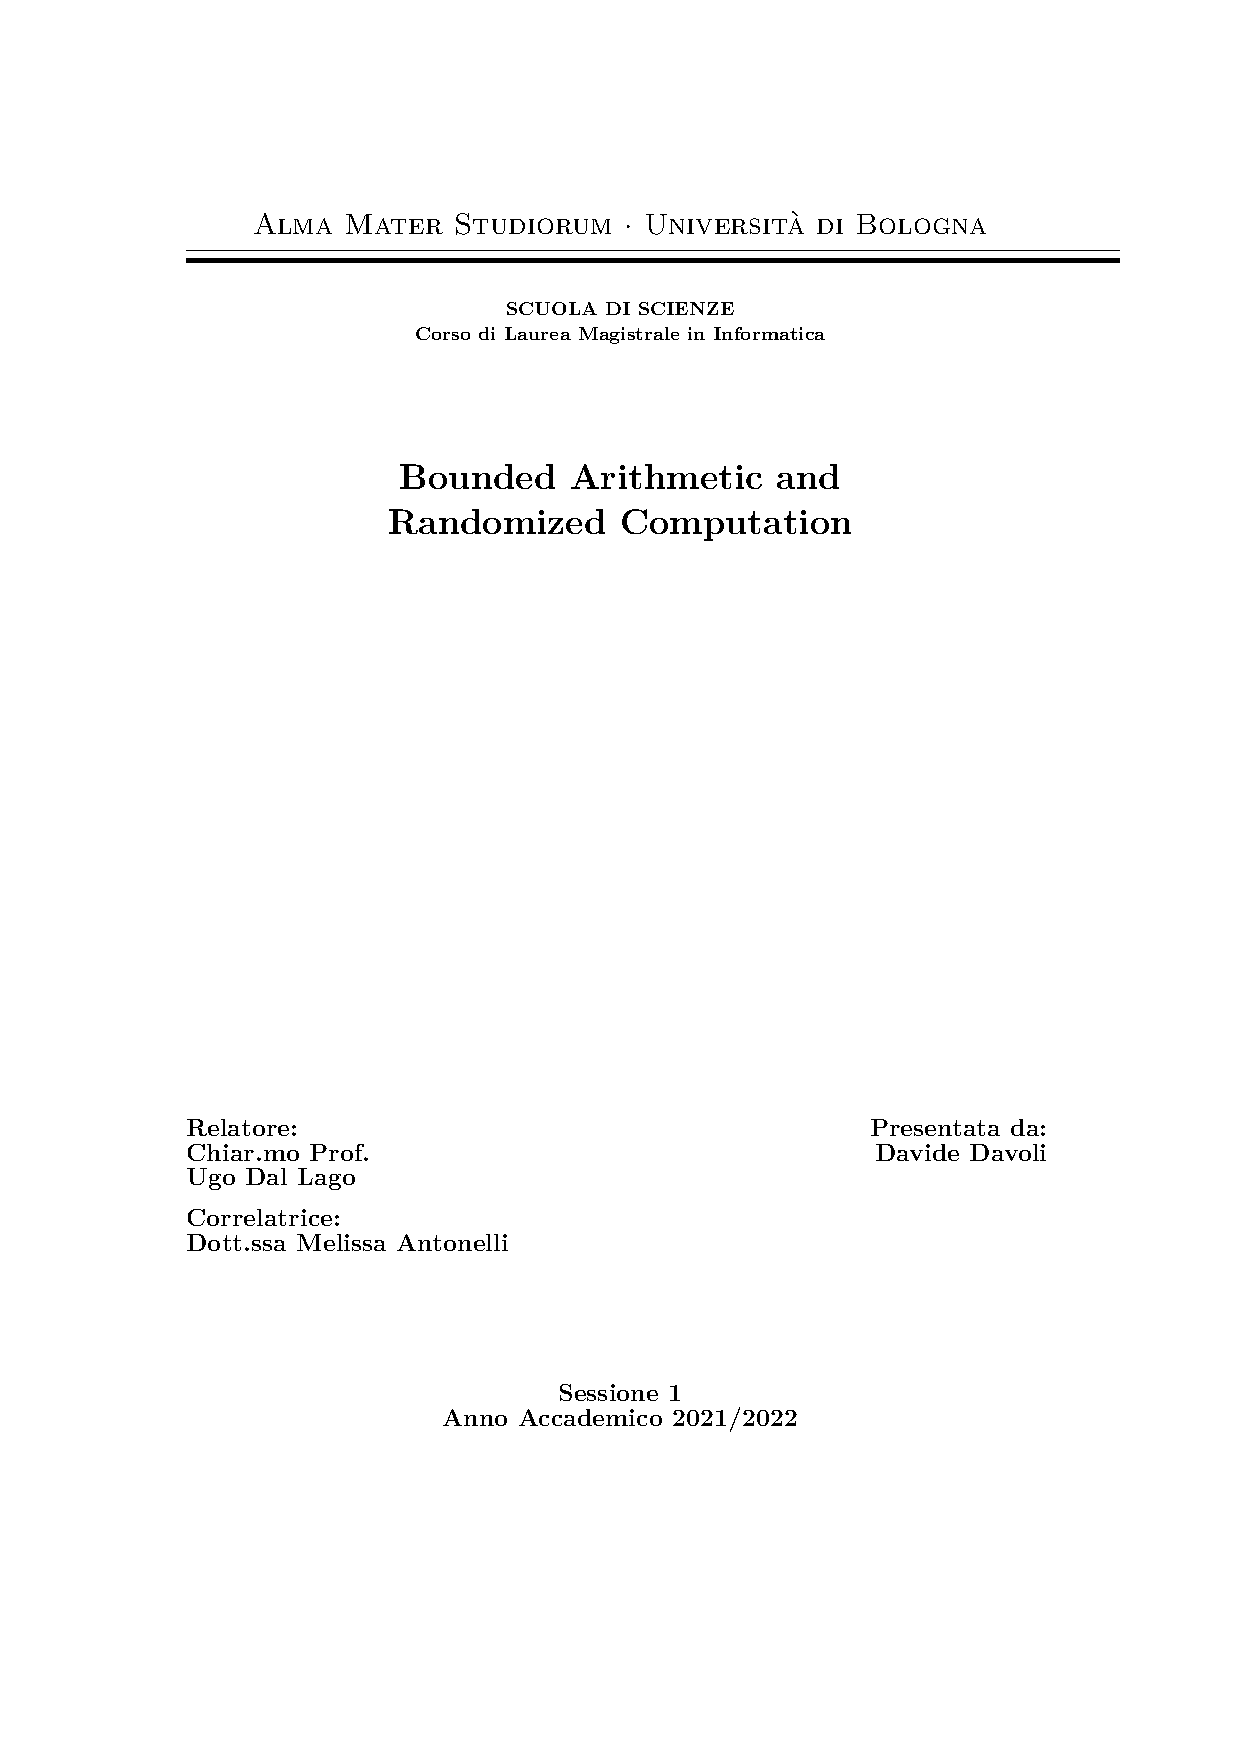
\includepdf{titlepage}
% \begin{titlepage}
% \thispagestyle{empty}
% \begin{center}
% {{\Large{\textsc{Alma Mater Studiorum $\cdot$ Universit\`a di
% Bologna}}}} \rule[0.1cm]{15.8cm}{0.1mm}
% \rule[0.5cm]{15.8cm}{0.6mm}
% {\small{\bf SCUOLA DI SCIENZE\\
% Corso di Laurea Magistrale in Informatica }}
% \end{center}
% \vspace{15mm}
% \begin{center}
%   {\LARGE{\bf Bounded Arithmetic and }} \\
%   \vspace{3mm}
%   {\LARGE{\bf Randomized Computation }
% }\\
% \end{center}
% \vspace{95mm}
% \par
% \noindent
% \begin{minipage}[t]{0.47\textwidth}
% {\large{\bf Relatore:\\
% Chiar.mo Prof.\\
% Ugo Dal Lago}\\[1.5ex]
% \large{\bf Correlatrice:\\
% Dott.ssa Melissa Antonelli}
% }
% \end{minipage}
% \hfill
% \begin{minipage}[t]{0.47\textwidth}\raggedleft
% {\large{\bf Presentata da:\\
% Davide Davoli}}
% \end{minipage}
% \vspace{20mm}
% \begin{center}
% {\large{\bf Sessione 1\\%inserire il numero della sessione in cui ci si laurea
% Anno Accademico 2021/2022}}%inserire l'anno accademico a cui si è iscritti
% \end{center}
% \end{titlepage}


\def\level{\lextended}

\chapter*{Acknowelgements}
%!TeX spellcheck = en-US
I would like to express my sincere gratitude to my esteemed supervisor Prof. Ugo Dal Lago
whom has guided me through this research with patience, kindness and enthusiasm.
Together with Ugo, I would also like to express my gratefulness
to my co-supervisor Dr. Melissa Antonelli, for her great willingness
to help me complete this work.
Together with them, I am also thankful to Dr. Paolo Pistone and Prof. Isabel Oitavem
for the cordiality and for their assistance at every stage of the research project.
%
A wholehearted praise goes to my father Gianni for
the immense trust he has in me and to my mother, Patrizia,
who could not see neither
the beginning nor the end of many things I did, but
yet inspires many of them.
%
Finally, my sincere gratitude goes to my loved ones for supporting me every time
and filling my days with glee.


\tableofcontents

\chapter*{Introduction}
%!TeX spellcheck = en-US
At a broad level, Logic relies on proofs, which are assessments of an entailment between some premises and a consequence. Proofs are, ultimately, syntactical objects relating some formul\ae{} --- the \emph{premises} --- to another formula --- called \emph{consequence} --- according to some system of rules, called proof system.

Similarly, Computer Science is founded on the notion of program. Again, programs are syntactical objects, relating some input data with an output. Even programs, for being accepted by the compiler, must follow a system of rules called type system.

The correspondence between programs and proofs --- and at the higher level the correspondence between types and formul\ae{} --- grounds the so-called Curry-Howard isomorphism \cite{curry34, Howard}. This relation brings fruitful contributions to both the fields of Computer Science and logic. In Computer Science, for example, it is possible to shape computational formalisms upon well-behaved logics. These formalisms, for instance, are particularly suited for program analysis because of their solid logical properties. On the side of Logic, this correspondence makes it possible to represent proofs by means of computer programs, reducing the act of deducing a proof to the act of coding a well typed function.

Another consequence of this correspondence is the possibility to approach computational complexity by means of peculiar logical theories, called bounded srithmetics.
%
These are basically first-order logical theories generated by four elements: a logical language $\mathcal L$, its semantics $\llbracket \cdot\rrbracket$, a set of axioms $A$ and a proof system $\vdash$, which are capable to capture well known classes of program --- often complexity classes --- relating them with collections of foruml\ae{}.
%
This relation is grounded on the notion of provability: each derivation rule has a well known corresponding computation step. Thus, a program --- i.e. a sequence of computational steps --- can be represented by means of a proof, which is a sequence of deduction rules. For this reason, within a bounded arithmetics it si possible to identify certain \emph{provable formul\ae{}} which correspond to computable functions.
%
Tailoring this theory --- or, more often, its language $\mathcal L$ and the set of its axioms $A$ --- it is possible to identify, within a bounded arithmetic, classes of formul\ae{} which correspond to well-known complexity classes.

In his PhD thesis \cite{Buss86}, S. Buss managed to develop a bounded arithmetic which characterizes the complexity class $\FP$. Precisely, Buss proved that every polynomial-time computable function corresponds to a function which is $\Sigma^b_1$-definable in the corresponding bounded theory $S^1_2$ \cite{Buss86}. This result is very insightful, but no similar works have been proposed in the realm of probabilistic computation, yet.

In contrast with deterministic computation, the probabilistic framework allows the computational models --- canonically \emph{Probabilistic Turing Machine} --- to take purely random choices in each step of its computation. Thus, in this setting, reduction becomes a stochastic process, and the semantics of a program can no more be reduced to a function mapping inputs to outputs. Instead, it becomes a function which associates to any input a distribution of probability over its possible outputs.

The probabilistic framework has some relevant advantages with respect to the deterministic one: in particular, random choices allow to approximate solutions to problems with smallest average case time consumption and arbitrarily low error. This is evident if we examine the complexity class $\BPP$, which contains all the decision problems having a probabilistic poly-time algorithm solving them with arbitrarily low error, and thus is intended to capture \emph{feasibility} in probabilistic computation. Indeed, there are problems which are in $\BPP$, but which are yet not known to be in $\mathbf P$. For instance, the probabilistic algorithm for solving the Polynomial Identity Test is not known to have any solution in $\mathbf P$, but it is known to have one in $\BPP$.
%
As for $\mathbf {NP}$, there are open problems concerning $\mathbf {BPP}$ and $\mathbf P$. The most important is probably $\mathbf P = \BPP$, indeed many problems in $\BPP$ have been recently discovered being in $\mathbf P$ such as, for example, the Primality Test.

Since November 2021 I am involved in a joint research project with
Prof. Ugo Dal Lago, Dr.
Paolo Pistone and Dr. Melissa Antonelli
from University of Bologna
and with Prof. Isabel Oitavem from NOVA University of Lisbon, Portugal.
%
%
The contribution of our work consists precisely in extending Buss' work to the study of probabilistic complexity classes.
The basic idea is to generalize $S^1_2$'s language and semantics to a quantitative setting. Concretely, the first step consists in relating bounded formul\ae{} with some effective model for probabilistic computation.

For this purpose, we introduced three novel classes of functions and prove them equivalent:

\begin{enumerate}
\item The class of
\emph{polynomial-time oracle recursive functions} ($\POR$),
which is a Cobham style function algebra \cite{Cobham1965}, with the
capability to query an \emph{oracle-function}
$\omega: \{\zero, \one\}^* \longrightarrow \{\zero, \one\}$ to
\emph{possibly random} bits during the evaluation.

\item The class of functions which are
$\Sigma^b_1$-representable in $\RS$,
where $\RS$ are di axioms of our \emph{randomized bounded theory}.
%
This theory is expressed in a  ``probabilistic
word language'', %$\mathcal{L}_{\mathbb{W}}$,
%the intended interpretation of which is the class
%of $\mathbf{0}$-$\mathbf{1}$ strings.
%
which is a canonical first-order
%$\mathbf{0}$-$\mathbf{1}$
word language with equality inspired from~\cite{FerreiraOitavem}, augmented
by a special unary ``probabilistic'' predicate $\Flip(\cdot)$~\cite{ADLP21}.
%
%Inspired by $\MQPA$, we also introduce  a quantitative semantics such that  formul\ae{} in $\mathcal{L}_{\mathbb{W}}$ are associated to (measurable) sets of strings.
%
%Then, $\RS$ is defined as a \emph{bounded} theory very close to Buss's $S^1_2$~\cite{Buss} and Ferreira's $\Sigma^b_1$-NIA~\cite{Ferreira88,Ferreira90}.
%
%We also slightly modify the standard notion of $\Sigma^b_1$-representability so to deal with our theory, as defined in a probabilistic word language, and our class $\POR$ of oracle functions over strings (and not over natural numbers). (It is in this context the quantitative interpretation of $\mathcal{L}_{\mathbb{W}}$ becomes crucial.)



\item The class of \emph{$\SFP$-functions},
which is the class of functions computable by
%$\SFP$-machines, i.e.
polynomial-time
Stream Machines.
%
These are almost ordinary $k+1$-taped
Turing machines; the only difference is that
one of their tapes,
called the \emph{oracle tape},
is used as a left-to-right read-only tape
and contains an infinite sequence of random bits.
%
These machines differ from standard probabilistic Turing
machines~\cite{Santos69,Gill77},
as their access to randomness is close to
that of $\POR$'s functions: their computation depends on
a function $\eta: \Nat \longrightarrow \{\zero, \one\}$ which
describes the configuration of the \emph{oracle tape}.
%

\end{enumerate}



%
%
%
%
%
%
%
%Then, we prove that  functions in $\POR$ are precisely those in $\SFP$ in two main steps:
%We prove that each poly-time oracle function are precisely the $\Sigma^b_1$-representable ones.
%We generalize Cobham's result showing that  functions in $\POR$ are precisely those in $\SFP$.
%

Our main result consists in proving
that the class of functions which are
$\Sigma^b_1$-representable in $\RS$
is precisely the class of polynomial-time computable
ones which, in turn, coincides with the
class of $\SFP$-functions.
%
%In this way, we manage to represent in our logical system the desired  probabilistic computational model and to deal with formula expressing.
%
%Together with the notion of measure-quantifiers, this allows us to switch to a probabilistic model of computation to provide (semantic) characterizations of probabilistic classes.
%
%For example, one can imagine to characterize a class of probabilistic functions, for example the one corresponding to problems in $\BPP$~\cite{AroraBarak}, using (a special, simple kind of) formul\ae{} of $\MQPA$ to generalize (ii) below with a condition satisfied with respect the appropriate bound, in the case of $\BPP$ as $\BOX^{2/3}A(x,f(x))$.
%
Then, starting from this equivalence,
it seems possible to characterize probabilistic classes,
such as $\BPP$ or $\ZPP$,
using formul\ae{} of the bounded theory $\RS$
together with non-standard quantifiers.
%
For instance, functions corresponding to problems
in $\BPP$ could be characterized leveraging a
measure-sensitive quantifier $\BOX$ in the style of $\MQPA$, \cite{ADLP,ADLP21}.
%

In this work, I will describe the main advances we have made to this end,
primarily focusing on my personal contributions which
are the reductions from $\POR$ to $\SFP$,
and vice-versa, the equivalence between $\SFP$ and $\PPT$,
A logical characterization of some probabilistic complexity classes.

The thesis is structured as follows: in Chapter \ref{chap:preliminaries},
I recall describe the scientific context of this work,
recalling some basic probability notions together, together with Buss'
Bounded Arithmetic, then in Chapter \ref{chap:RBA}, the $\RS$ is defined
together with the $\POR$ function algebra and a representability result between
the two classes. Later, I will focus on my personal contributions to this research:
in Chapter \ref{chap:sfptopor}, I investigate the equivalence between $\POR$ and
the class of functions which are computable in polynomial time by a Probabilistic
Turing Machine, i.e. $\PPT$. Thus, I generalize the main result of Chapter \ref{chap:RBA}
Showing that the $\RS$ representable functions are exactly the $\PPT$ ones.
In Chapter \ref{chap:cobham}, I show that the equivalence between $\POR$ and
$\PPT$ has, as corollary, the equivalence between a Cobham-style function algebra ---
thereby introduced and called $\polyF$ --- and the complexity class $\FP$. Finally, Chapter
\ref{chap:characterization} contains the characterizations of some standard
probabilistic complexity classes by means of a semantical condition expressed
in a word language $\Lmq$ inspired by $\Lpw$ and $\MQPA$.


\chapter{Preliminaries}
\label{chap:preliminaries}
%!TeX spellcheck = en-US

Before getting into the main concern of this thesis --- i.e. the development
of a bounded arithmetic for randomized computation --- we would like to
briefly recall some some standard notions which are nevertheless fundamental
for our work.
%
To this aim, within the following sections, we will fix the notation for
standard Turing Machines, recall some basic results
of Probability and Measure
Theory,
describe some basic aspects of the probabilistic computational paradigm and, finally,
we will recall the main results of S. Buss' bounded arithmetic.
%
However,
these sections each one independent from the others and
none of them contains peculiar details affecting the following part of this
work. For these reasons, the reader that feels confident on these subject
can directly jump to the next chapter, in which we define our Randomized
Bounded Arithmetic and prove it equivalent to the thereby introduced $\POR$
function algebra.















\section{Turing Machines}

In this section, we define Turing Machines. This is aimed to
fix the notation of all the similar computational paradigms which will be introduced
in what follows.
% For sake of consistecny with the other
% models Turing-like machines defined in this work, even in this case
% we will follow the same approach
% used in the definition of STMs: for instance, the head will
% write the character on its immediate right, and we will not make use of final states.

%%% DEFN Stream Turing Machine
\begin{defn}[Turing Machine]\label{df:TM}
A \emph{Turing machine} is a quadruple
$M:= \langle \m{\Qs}, \m{q_0}, \m{\Sigma}, \m{\delta} \rangle$, where:
\begin{itemize}
\itemsep0em
\item $\m{\Qs}$ is a finite set of states ranged over by
$\m{q_i}$ and similar meta-variables.
%
\item $\m{q_0} \in \m{\Qs}$ is an initial state.
%
\item $\m{\Sigma}$ is a finite set of characters
ranged over by $\m{c_i}$ \emph{et simila}.
%
\item $\m{\delta}: \m{\hat{\Sigma}}
\times \m{\Qs}
\longrightarrow \m{\hat{\Sigma}} \times \m{\Qs} \times \m{\hat{\Sigma}} \times \{\m{L},\m{R}\}$
is a transition function describing the new configuration
reached by the machine,
\end{itemize}
where  \m{$L$} and \m{$R$} are two fixed and distinct symbols,
e.g.~\m{$\zero$} and \m{$\one$},
$\m{\hat{\Sigma}}=\m{\Sigma} \cup \{\m{\blank}\}$
and \m{$\blank$} represents the
\emph{blank character}, such that $\m{\blank} \not \in
\m{\Sigma}$.
\end{defn}
%
\noindent
As for other flavors of Turing machines of this work,
without loss of generality, we will take in exam single-taped machines
with a binary alphabet only.
%
%
%
%
%%% Notation
%\begin{notation}
%In the following, let us use $\m{c}_{|\m{\Sigma}|+1}$ to denote the blank character $\m{\blank}$.
%\end{notation}
%
%
%
The \emph{configuration} of a ordinary TM is
a tuple which keeps track of the current state
and some strings representing the state of the
machine tape(s).


%%% DEFINITION
%%% CONFIGURATION
\begin{defn}[Configuration of a TM]\label{df:TMConfiguration}
The \emph{configuration of a TM}
is a triple $\langle \m{\sigma},
\m{q}, \m{\tau}\rangle$,
where:
\begin{itemize}
\itemsep0em
%
\item $\m{\sigma} \in \hat{\Sigma}^*$
is the portion of the work tape on the left of the head;
%
\item $\m{q}\in A$ is the current state of the machine;
%
\item $\m{\tau} \in \hat{\Sigma}^*$ is the portion of the
work tape on the right of the head.
%
\end{itemize}
\end{defn}
%
%
\noindent
The shift of the tape is naturally defined by
pre-fixing and post-fixing characters to strings
%
%
%
%
%
The dynamic behavior of a TM is defined
recurring to a transition function.


%%% DEFINITION
%%% STM Transition Function
\begin{defn}[TM Transition Function]\label{df:TMTransition}
Given a TM, $M=\langle
\m{\Qs}, \m{q}, \m{\Sigma}, \m{\delta}\rangle$,
we define the \emph{partial transition function}
$\tmtrans \delta: \hat{\Sigma}^* \times
\Qs \times \hat{\Sigma}^* \longrightarrow
\hat{\Sigma}^* \times
\Qs \times \hat{\Sigma}^*$
between two configurations as:
%
\begin{align*}
\langle \m{\sigma}, \m{q}, \m{c\tau}\rangle
%
\tmtrans_{\delta}
%
\langle \m{\sigma c'}, \m{q'}, \m{\tau}\rangle
%
\ \ \ \ \ &\text{if} \ \m{\delta}(\m{q},\m{c}) =
\langle \m{q'}, \m{c'}, \m{R}\rangle \\
%
%
%
\langle \m{\sigma c_0},
\m{q}, \m{c\tau}\rangle
\tmtrans_{\delta}
\langle \m{\sigma},
\m{q'}, \m{c_0c_1'\tau}\rangle
%
\ \ \ \ \ &\text{if} \ \m{\delta}(\m{q}, \m{c_1}) = \langle
\m{q'}, \m{c_1'}, \m{L}\rangle.
\end{align*}
%
\end{defn}
%
%
%
\noindent
The transitive closure of $\tmtrans$ yields the reachability
function between configurations of the machine, as defined below:

%%% DEFINITION
%%% REACHABILITY FUNCTION

\begin{defn}[TM Reachability Function]\label{df:TMReachability}
Given a TM,
$M=\langle \m{\Qs}, \m{q_0}, \m{\Sigma}, \m{\delta}\rangle$,
$\{\tmreach^n_M\}_n$ is the smallest
family of relations such that:
%
%
%
\begin{align*}
\langle \m{\sigma}, \m{q}, \m{\tau}\rangle
&\tmreach^0_M
\langle \m{\sigma}, \m{q}, \m{\tau}\rangle \\
%
%
\big(\langle \m{\sigma}, \m{q}, \m{\tau}\rangle
\tmreach^n_M
\langle \m{\sigma'}, \m{q'}, \m{\tau'}\rangle\big)
%
\wedge
%
\big(\langle \m{\sigma'}, \m{q'}, \m{\tau'}\rangle
%
&\tmtrans_\delta
%
\langle \m{\sigma''}, \m{q''}, \m{\tau''}\rangle\big)
\rightarrow
\big(\langle \m{\sigma}, \m{q}, \m{\tau}\rangle
\tmreach^{n+1}_M
\langle \m{\sigma''}, \m{q''}, \m{\tau''}\rangle\big).
\end{align*}
\end{defn}
%
%
%
%
\noindent
Even in this case, without loss of generality,
we assume that TMs do not use final states:
computation is regarded as concluded
whenever the transition function
is undefined on the current configuration.


\begin{prop}\label{proptm}
For any TM,
$M=\langle \m{\Qs}, \m{q_0}, \m{\Sigma},\m{\delta}\rangle$
and $n\in \Nat$,
$\tmreach^n_M$ is a \emph{partial} function.
\end{prop}
\begin{proof}
  Trivial, by the fact that $\tmtrans$ is a function and because
  the composition of two functions is a function, too.
\end{proof}













\begin{notation}[Final Configuration]
Given a TM,
$M=\langle \m{\Qs}, \m{q_0}, \m{\Sigma}, \m{\delta}\rangle$,
and a configuration
$\langle \m{\sigma}, \m{q}, \m{\tau}\rangle$,
we write
$\langle \m{\sigma}, \m{q}, \m{\tau}\rangle \not\tmtrans_{\delta}$
when there are no $\m{\sigma'}, \m{q'}, \m{\tau'}$
such that
$\langle \m{\sigma}, \m{q}, \m{\tau}\rangle
\tmtrans_{\delta} \langle \m{\sigma'}, \m{q'},
\m{\tau'}\rangle$.
\end{notation}
%
%
%
\noindent
Finally, let us introduce the notion of function computable by TMs.





%%% COMPUTATION of STM
\begin{defn}[TM Computation]\label{def:TMcomputation}
Given a TM,
$M = \langle \m{\Qs}, \m{q_0}, \m{\Sigma}, \m{\delta}\rangle$
and a function $g: \Ss \longrightarrow \Ss$,
we say that
\emph{$M$ computes $f$}, written $f_M = g$ if and only if
for every string $\sigma\in \Ss$,
there are $n\in \Nat$
and a $\m{\tau}\in \Ss, \m{q'} \in \Qs$,
such that:
$$
\langle \m{\eepsilon}, \m{q_0}, \m{\sigma}\rangle
\ \tmreach^n_M \
\langle \m{\gamma}, \m{q'}, \m{\tau}\rangle
\not\vdash_{\delta},
$$
%for some $\m{\tau}, \m{q'$} and $\m\psi$ and
with $f(\sigma)$ being
the longest suffix of $\m{\gamma}$ not including
$\m{\blank}$.
\end{defn}




\begin{defn}[Poly-Time Turing Machine]\label{df:PTM}
A \emph{poly-time stream Turing machine}
is an TM,
$M= \langle \m{\Qs}, \m{q_0}, \m{\Sigma}, \m{\delta}\rangle$
such that:
$$
\exists p\in \textsf{POLY}.
\forall \m{\sigma} \in \Ss,
\eta \in \Bool^\Nat.
\exists n \leq p(|\m{\sigma}|)
\big(\langle \m{\eepsilon},
\m{q_0}, \m{\sigma}, \m{\eta} \rangle
\tmreach^n_{M}
\langle \m{\gamma}, \m{q'}, \m{\tau}, \m{\psi}\rangle \not\vdash_{\delta}.
$$
\end{defn}
%
%
\noindent
We define the class of functions which
are computable by poly-time TMs.


%%% The Class SFP
\begin{defn}[The Class $\FP$]\label{df:FP}
$$
\FP := \{ f \in \Ss \times \Bool^\Nat \ | \
f = f_{M}\text{ for some polynomial TM, $M$}\}
$$

\end{defn}
%
%
\noindent












\section{On Measure Theory and Probability Thery}

This section is aimed to introduce some basic notions and notations of Measure
and Probability theory with the aim to
the introduction of those basic technical notions which will be necessary to follow
the following discussions.
%
The reader who is interested in a deeper and complete introduction
to Probability Theory can consult Feller's
``An Introduction to Probability Theory and its Applications'' \cite{feller1968introduction}
or Billingsley's  ``Probability and Measure'' \cite{Billingsley}.
%
In particular, Billingsley's work has been taken as a reference in many parts of this work.

Probabilities studies how it is possible to \emph{measure} the degree of certainty of some events.
Let $\Omega$ be an arbitrary set of events.
In Probability Theory, the algebra of sets describing probabilistic events and their composition is called a ``field''.

\begin{defn}[Field]
  A filed $\mathcal F$ is a pair $\langle \Omega, F\rangle$ such that $F \subseteq \mathcal P(\Omega)$ and:
  \begin{itemize}
    \item $\Omega \in F$;
    \item $X \in F \to \overline X \in F$;
    \item $X \in F \land Y \in F \to  X \cap Y \in F$.
  \end{itemize}
\end{defn}

\noindent
Due to the presence of complementation, observe that the third
condition in the definition of a field could be restated
recurring to intersection rather than set
union, obtaining an equivalent definition. This result can be
trivially shown by induction on the proof that a set belongs to a
specific field.
%
Moreover, we would like to point out that the elements of a field can only be finite or co-finite with respect to $\Omega$.

If we relax this finitary condition, we end up defining a different
algebraic structure, called $\sigma$-field, or $\sigma$-algebra.

\begin{defn}[$\sigma$-field]
  A $\sigma$-field $\Sigma$ is a set $\Sigma \subseteq P(\Omega)$ such that:
  \begin{itemize}
    \item $\Omega \in F$;
    \item $X \in F \to \overline X \in F$;
    \item $X_1, X_2, \ldots \in \Nat. \to \bigcup_{i \in \Nat} X_i \in F$.
  \end{itemize}
\end{defn}

\noindent
If $\Sigma$ is a $\sigma$-field, then the pair $\langle \Omega,
\Sigma\rangle$ are called \emph{measurable spaces}. This epithet is due to
the possibility to use these sets to define measure functions $\mu:
\Sigma \longrightarrow \mathbb R$, peculiar functions associating a
real number to each set.


The elements of a $\sigma$-field intuitively represent all the possible
outcomes of a random experiment and, within a probabilistic context,
are called \emph{events}. Thus, assignment of a degree of certainty to each possible random event can be accomplished by defining a function
which assigns to each element of a $\sigma$-field a value, representing
the certainty of that event.
%
However a function, in ordered to be a \emph{measure function},
must verify some constraints
upon its values.

\begin{defn}[Measure Function]
  If $\langle \Omega, \Sigma\rangle$ is a measure space, then a function $\mu: \Sigma \longrightarrow \mathbb R$ is a \emph{measure function} if and only if:
  \begin{itemize}
    \item $\forall X \in \Sigma. \mu(X)\ge 0$;
    \item $\mu(\emptyset)=0$;
    \item For all the countable collections $\{X_i\}_{i \in \Nat}$, if all the $X_i$ are pairwise disjoint, then:
    $$
    \mu\left (\bigcup_{i \in \Nat} X_i \right)= \sum_{i \in \Nat}\mu(X_i).
    $$
  \end{itemize}
\end{defn}

However, there is a class of measure functions
with stronger constrains which are those actually employed Probability Theory
to measure the degree of certainty of probabilistic events.
% following with the definition
% of a field containing all the possible events, we are also interested
% in defining a function which assigns a degree of certainty to each possible event within the field.

\begin{defn}[Probability Measure]
  If $\mathcal F := \langle \Omega, F\rangle$ is a field and $P: \Sigma \longrightarrow \mathbb R$, then $P$ is a probability measure if and only if:
  \begin{itemize}
    \item $\forall X \in \Sigma. 0 \le  \mu(X)\le 1$;
    \item $\mu(\emptyset)=0 \land\mu(\Omega)=1$;
    \item For all the countable collections $\{X_i\}_{i \in \Nat}$, if all the $X_i$ are pairwise disjoint, then:
    $$
    \mu\left (\bigcup_{i \in \Nat} X_i \right)= \sum_{i \in \Nat}\mu(X_i).
    $$
  \end{itemize}
\end{defn}

\begin{remark}
  All the probability measures are measures, while the converse does not hold.
\end{remark}

These are all the ingredients we need to define a probability space:

\begin{defn}[Probability Space]
  If $\langle \Omega, \Sigma\rangle$ is a measurable space and $P$,
  then the triple $\langle \Omega, \Sigma, P\rangle$ is called
  \emph{Probability Space}.
\end{defn}

Events by themselves are the pure outcome of a probabilistic
experiment. For this reason it is often useful to
define functions associating each possible
event to a generical interpretation. These functions are called ``random variables''.

\begin{defn}[Random Variable]
  If $\langle \Omega, \Sigma, P\rangle$ is a probability space and
  $K\neq \emptyset$ is a set, a function $Z: \Omega \longrightarrow K$
  is a random variable.
\end{defn}

As for ordinary events, it is possible to associate a degree of
certainty to each possible value assumed by a random variable. This
is simply done recurring to the measure of their pre-image.

\begin{defn}[Probability of a Random Variable]
  If $\langle \Omega, \Sigma, P\rangle$ is a probability space and
  $Z: \Omega \longrightarrow K$ is a random variable,
  then we define the probability distribution of the variable $Z$ as the function $\mathit{Pr}: K \longrightarrow [0,1]$ defined as follows:
  $$
  \mathit{Pr}[Z = k] = P(Z^{-1}(\{k\})).
  $$
  Fixed a set $K$, we call $\mathbb D(K)$ the set of all the probability distributions over $K$.
\end{defn}

These few notions are everything required to walk through the
probabilistic concerns of this work. For a better understanding of
these notion, we take in exam a school-book like example of
probability theory:

\begin{ex}
  Let us build a model for the experiment of rolling a dice, in order to determine the probability of getting an outcome which is greater or equal than $4$. Then, the set $\Omega$ of all the possible outcomes of the experiment can be defined as $\Omega:=\{1,2,3,4,5,6\}$.
  Basing on $\Omega$, we can define a probability space as follows:
  \begin{itemize}
    \item $\Sigma:=\mathcal P (\Omega)$;
    \item $P:=X \mapsto \frac{|X|}{|\Omega|}$.
  \end{itemize}
  The triple $\langle \Omega, \Sigma, P\rangle$ is a probability
  space: indeed $\Sigma$ is a finite $\sigma$ algebra on $\Omega$ and
  $P$ is a probability measure.
  Finally, our experiment can be modeled by means of the random
  variable $Z: \Omega \longrightarrow \{0, 1\}$ defined as follows:
  $$
  Z(x):= \begin{cases}
  1 & \text{ if }x\ge 4\\
  0 & \text{ otherwise. }
  \end{cases}
  $$
  Finally, we can quantify $\mathit{Pr}[Z=1]$ as follows:
  $$
  \mathit{Pr}[Z=1]=P(Z^{-1}(1))=P(\{4, 5, 6\})= \frac{|\{4, 5, 6\}|}{|\Omega|}= \frac 3 6 = \frac 1 2.
  $$

\end{ex}





\section{Randomized Computation}

Standard deterministic computation is defined upon TMs.
This computational model features all the
capabilities of a standard calculus formalism, indeed, as meant by Alan Turing,
computation can be represented as a process of rewriting some expressions
following predefined rules~\cite{rogers1987theory}.
%
However, although the TM computational model is sufficiently
expressive to shape mathematical computations, it is still not capable to
capable to model \emph{purely random events}.

Even though the existence of randomness is itself debatable, there
are real world experiments --- such as a coin toss, for instance ---
whose outcome is sufficiently uncertain to be considered random  for practical purposes.
%
Thus, it makes sense to consider computational models which, during
the computation, may take purely random choices.
%
Random algorithm are nowadays pervasive in many fields of Computer Science,
such as Cryptography, Numerical Analysis and Machine Learning.

Intuitively, the output of a random algorithm \emph{can be}
uncertain. Thus, if a random algorithm is employed to solve a
problem, the solution it proposes \emph{can be} uncertain ---
and, in many cases, it is.
%
For an algorithm, producing  uncertain or approximated solutions is not an advantage,
especially if this feature is considered by itself. However,
sometimes probabilistic algorithms can solve computationally
hard problems with simple algorithms, low error and lower time
complexity than any non-random solution.
In the Introduction, we have already mentioned some of
these cases: the Polynomial Identity Testing Problem (PIT) and the Primality Test.
While PIT is known to be in $\BPP$,
there is no evidence of this problem being in $\mathbf P$; contrarily the
Primality Test problem has been shown being in both $\BPP$ and $\mathbf P$,
but the time consumption of the probabilistic Miller Rabin Test
on is sensibly lower than the AKS
algorithm which is up to now, the fastest non-random algorithm \cite{shoup2009computational}.
% In what follows, we will take in exam the Primality Test problem in order to
% show how admitting a rather small probability of code
% allows to solve complex problems efficiently.
%
In complexity theory, the trade-off between approximation and time
consumption leads to the definition of complexity classes which
capture a new notion of feasibility based on Random Computation.

Within this section, we introduce the definition a of a
computational model for randomized computation and we define some
complexity classes which model a probabilistic notion of
feasibility, discussing their inter-relations and properties.

\begin{restatable}[Probabilistic Turing Machines \cite{AroraBarak}]{defn}{defptm}
  \label{def:ptminformal}
A \emph{probabilistic Turing machine}
is a Turing machine with two transition functions, namely $\delta_0,\delta_1$.
%
Given an input $x$, the PTM chooses at each step
with probability $\frac{1}{2}$ to apply
the transition function $\delta_0$ and with the same probability to apply $\delta_1$.
%
This choice is independent from all the previous ones.
\end{restatable}

To model the semantics of a Probabilistic Turing Machines (PTM, for short),
we cannot recur to functions from strings to strings, because the output
of the computation is the outcome of a stochastic process, so it results in
a probability distribution. Indeed, called $\Ss$ the set of binary strings, the semantics
of a PTM is a function
$$
f: \Ss \longrightarrow \mathbb D (\Ss).
$$
\noindent
Within the class of PTM-computable functions, we can identify a thinner class
imposing a polynomial time bound: the class of $\PPT$ functions.

\begin{restatable}[Class $\PPT$]{defn}{defppt}
  \label{def:pptinformal}
The \emph{class $\PPT$} is the class of random functions
from $\Ss$ to $\mathbb D(\Ss)$
which are computable by a PTM in at most a polynomial
number of steps.
\end{restatable}

Notice that when defining $\PPT$ we could make a slightly different requirement on the time complexity of those functions: indeed, we could require their \emph{expected} time consumption to be at most polynomial. This dichotomy is pervasive in probabilistic complexity: usually, algorithm with \emph{worst case} time bounds are called \emph{Monte Carlo} algorithm, while algorithm with \emph{average case} time bounds are usually called \emph{Las Vegas} algorithms.

Characterizing feasible decisional problem by means of
probabilistic algorithms, we are interested
in two properties of these procedures: of course we re interested
polynomial time complexity ---
which can be captured by the $\PPT$ class --- but we also want to impose
limitations to the amount of error these algorithms can make.
%
An example of how it is possible to capture both these property is the
\emph{Bounded error Probabilistic Poly-time} complexity class $\BPP$.

\begin{restatable}[Class $\BPP$]{defn}{defbpp}
  \label{def:bppinformal}
We say that a language $L\subseteq \Ss$ is in $\BPP$ if and only if,
said $f_L$ the characteristic function of the language,
there is a $\PPT$ function $f$ such that:
$$
\forall x \in \Ss.\mathit{Pr}[f(x)=f_L(x)]\ge \frac 2 3.
$$
\end{restatable}

One can argue that $\frac 1 3$ of wrong detections
can not be considered \emph{low error}. However, we must also take in account
that, since it is possible to evaluate the same probabilistic function multiple
times, it has been shown that the amount of error of a $\BPP$ function can
be reduced arbitrarily preserving the program's poly-time consumption,
\cite[Lemma 7.9]{AroraBarak}.
%
The class $\BPP$ is usually referred to as a \emph{double sided error} class.
Indeed the probability of error is equal for all the strings which are in the language
and those who are not.
%
One may also be interested in studying randomized algorithms which do not allow
false positive or false negatives or even both of them. These three possibility
represent three different nuances of feasibility within the probabilistic
framework. Any of them is captured by a different complexity class.

\begin{restatable}[Class $\RP$]{defn}{defrp}
  \label{def:rpinformal}
We say that a language $L\subseteq \Ss$ is in $\RP$ if and only if
there is a
$\PPT$ function $f$ such that:
\begin{align*}
\forall \sigma \in L. Pr[f(\sigma) = \one]\ge \frac 2 3\\
\forall \sigma \not\in L. Pr[f(\sigma) = \zero]= 1.
\end{align*}
\end{restatable}
\noindent
It is almost trivial to see that $\RP$ is included within $\BPP$:
take an $\RP$ function $f$ deciding $L$:
the probability of error of $f$ is always
smaller than $\frac 1 3$, which is the definition of $\BPP$. Thus, $L \in \BPP$.

Usually, the complexity classes which are not trivially known to be closed
under complementation --- $\NP$ and $\RP$ are among those classes ---
cause the introduction of the class containing all the
complementations of their problems as a class as on its own. This
would be useless for classes which are closed under complementation, because that
novel class would be identical to the original one.

The complementary of $\RP$ is co-$\RP$ and is the class of
languages $L$ such that there is a $\PPT$ function $f_L$ accepting
the members of $L$
with no probabilistic error at all
and refusing the strings which not belonging to $L$
with probability of error smaller than $\frac 1 3$.
This is another example of \emph{one-sided} probabilistic error.
The definition of this class can be formally
stated as follows:

\begin{restatable}[Class co-$\RP$]{defn}{defcorp}
  \label{def:corpinformal}
We say that a language $L\subseteq \Ss$ is in co-$\RP$ if and only if
there is a
$\PPT$ function $f$ such that:
\begin{align*}
\forall \sigma \in L. Pr[f(\sigma) = \one]= 1\\
\forall \sigma \not\in L. Pr[f(\sigma) = \zero]\ge \frac 2 3.
\end{align*}
\end{restatable}

\noindent
Even in this case, one can observe that co-$\RP\subseteq \BPP$.
%
Finally one can be interested in stressing even more the error requirements
allowing no error at all. The complexity class thus obtained is called $\ZPP$
and contains all those languages which are known to
be solvable with no probabilistic error with polynomial time complexity,
which is quite peculiar, especially considering that the random choices
of the algorithm, for these programs do not cause any probabilistic outcome.
%
This even thinner complexity class is called $\ZPP$, which stands for \emph{``Zero Probabilistic Poly-time error''}.

\begin{restatable}[Class $\ZPP$]{defn}{defzpp}
  \label{def:zppinformal}
We say that a language $L\subseteq \Ss$ is in $\ZPP$ if and only if,
said $f_L$ the characteristic function of $L$,
there is a
$\PPT$ function $f$ such that:
\begin{align*}
  \forall \sigma \in \Ss. \forall \bool \in \{\zero, \one\} f(\sigma)=k &\to f_L(\sigma)=1 \\
  \forall \sigma \in \Ss. \mathit{Pr}[f(\sigma)\not\in \{\zero, \one\}]&< \frac 1 3.
\end{align*}
\end{restatable}
%
\noindent
In this definition, we require that the machine has no margin of error on all
its answer, however we admit the possibility that it in some cases it may output
a value different from $\zero$ and $\one$: this kind of answer should be interpreted as
``I do not know''. The definition of $\ZPP$ given above is not the standard one, but is an alternative characterization which requires the algorithm to be a \emph{Monte Carlo} algorithm rather than a \emph{Las Vegas} one. This because our Randomized Bounded Arithmetic characterizes the $\PPT$ functions, which are defined on top of \emph{Monte Carlo} algorithms, so this definition will allow a more natural characterization of such class in Chapter \ref{chap:characterization}.


It is possible to see that this class is included within $\BPP$, it is a consequence of
$\ZPP = \RP \cap \text{co-}\RP$, which we prove in Theorem \ref{thm:zpprpcorp1}.
This result also entails that $\ZPP$ is closed under complementation.

\begin{theorem}
  \label{thm:zpprpcorp1}
  $\ZPP = \RP \cap \text{co-}\RP$.
\end{theorem}
\begin{proof}
  We first show that $\ZPP \subseteq \RP \land \ZPP \subseteq \text{co-}\RP$.
  We examine only the second proposition: $\ZPP \subseteq \text{co-}\RP$.
  Let $f_L$ be the decision function for a language $L \in \ZPP$,
  take the following decision function for $L$:
  $$
  g(x) := \begin{cases} \one & \text{if } f(x)\neq \zero \land f(x)\neq \one \\ \zero & \text{otherwise.}\end{cases}
  $$
  Suppose that $\sigma \in L$, then $f(\sigma)=\one \lor (f(\sigma)\neq \zero \land f(\sigma)\neq \one)$,
  so $\mathit{Pr}[g(\sigma)=\one]=1$. Otherwise, assume that $\sigma \not \in L$
  $f(\sigma)=\zero \lor (f(\sigma)\neq \zero \land f(\sigma)\neq \one)$. In the first case,
  $g(\sigma)=\zero$, while in the second case $g(\sigma)=\one$ causing a wrong detection,
  but by definition of $\ZPP$, we know that it can happen with probability smaller than
  $\frac 1 3$. So $g \in \text{co-}\RP$. The proof that $\ZPP \subseteq \RP$ is analogous.
  Now we show that $\RP \cap \text{co-}\RP \subseteq \ZPP$.
  Suppose that $f_1$ is a $\PPT$ function such that $f_1(\sigma)=\one$ if $\sigma \in L$,
  and for $\sigma \not \in L$ $f_1(\sigma)=\one$ with probability smaller than $\frac 1 3$.
  Similarly, suppose that $f_2$ is a $\PPT$ function such that $f_2(\sigma)=\zero$ if $\sigma \not \in L$,
  and for $\sigma \in L$ $f_1(\sigma)=\zero$ with probability smaller than $\frac 1 3$.
  Then consider the $\PPT$ function $g$ defined as follows:
  $$
  g(x):=\begin{cases} f_1(x) & \text{if }f_1(x)=\zero\\
  f_2(x) & \text{if }f_2(x)=\one\\
  \one\one & \text{otherwise. }\end{cases}
  $$
  Suppose that $\sigma \in L$, then $g(\sigma)=\one\one$ only if $f_2(\sigma)=\zero$,
  which happens with
  probability smaller than $\frac 1 3$. Similarly, if $\sigma \not \in L$, then
  $f(x)=\one\one$ if and only if $f_1(\sigma)=\zero$, which happens with probability
  smaller than $\frac 1 3$.
\end{proof}

\begin{figure}[t]
  \centering
  \begin{tikzpicture}
    \node (BPP) {$\BPP$};
    \node[above left = 2cm and 2cm of BPP] (RP) {$\RP$};
    \node[below left = 2cm and 2cm of BPP] (coRP) {co-$\RP$};
    \node[left = 4cm of BPP] (ZPP) {$\ZPP=\RP\cap$ co-$\RP$};

    \draw[->] (ZPP) edge node[fill=white] {$\subseteq$} (RP);
    \draw[->] (ZPP) edge node[fill=white] {$\subseteq$} (coRP);
    \draw[->] (RP) edge node[fill=white] {$\subseteq$}  (BPP);
    \draw[->] (coRP) edge node[fill=white] {$\subseteq$} (BPP);

  \end{tikzpicture}
  \caption{Inclusion schema between complexity classes.}
  \label{fig:probcomp}
\end{figure}

\paragraph*{Considerations on Probabilistic Complexity Classes}

In the previous part of this section, we have shown some relations among
Probabilistic Complexity Classes. In particular we have shown how
$\BPP$, $\RP$, co-$\RP$ and $\ZPP$ are one included in the
other as described by Figure \ref{fig:probcomp}.
%
Moreover, Theorem \ref{thm:zpprpcorp1}, is a quite
surprising result: the corresponding question for
non determinism --- i.e. $\mathbf P = \NP\cap \text{co-}\NP$ --- is still open.

Another relation between probabilistic complexity classes and the non-probabilistic ones
is that $\BPP \subseteq \Sigma^p_2 \cap \Delta^p_2$, \cite{Goldreich}.
Thus if $\mathbf P = \NP$, then we would get $\mathbf P = \BPP$.
This motivates even more the interest in investigating these classes.

Despite these interesting inter-relations between non-probabilistic and
probabilistic complexity classes, we would like to point out that
the latter are inherently different
from the former:
they are considered \emph{semantic complexity classes}, instead of
\emph{syntactic complexity classes}.

Intuitively, all of those classes having a
procedure $c$ which decides whether the function computed by a given algorithm
$a$ passed as argument belongs or not to that class are considered syntactic complexity classes.
For example, $\mathbf P$ is a \emph{syntactic} complexity class,
because it suffices to take $c$ defined as follows:
$$
c(a):=\begin{cases} \one & \text{if }a\text{ is the encoding of a Timed Turing Machine with polynomial
time bound}\\ \zero &\text{otherwise.}\end{cases}
$$
Indeed, without lack of generality, one can consider every Timed Turing Machine as the
implementations of a \emph{decision} algorithm. A similar argument establishes,
for example, that $\mathbf {NP}$ is a \emph{syntactic} complexity class as well.
%
Conversely, classes which are not known to have this property are called
\emph{semantic complexity classes}.
For instance, take in exam $\BPP$:
it is not sufficient to check whether the algorithm $a$
is the encoding of a Timed Probabilistic Turing Machine with polynomial time bound.
Indeed, one must also assess that the probabilistic error
is bounder for every input. Unfortunately,
testing whether a given PTM has this property is not believed decidable, \cite{AroraBarak}.
Together with $\BPP$, even $\RP$, co-$\RP$ and $\ZPP$ are considered
\emph{semantic complexity classes}.

These considerations suggest that the analysis of probabilistic complexity classes
is intrinsically harder than the analysis of syntactical complexity classes, but that
due to the relations between probabilistic complexity classes and open problems
of Computer Science, the research in this field is surely worth its effort.


\section{Bounded Arithmetic}

A Bounded Arithmetic is a logical theory on a first-order language with identity, a preorder predicate symbol --- within this section we employ the symbol $\le$ ---, bounded quantifiers (Definition \ref{def:bussboundedquantifiers}) and some arithmetical functions.

\begin{defn}[Bounded Quantifier, \cite{Buss86}]
  \label{def:bussboundedquantifiers}
  A \emph{bounded quantifier} is a quantifier of the form $Qx \le t$ with
  $t$ a term not involving $x$. A \emph{sharply bounded quantifier} is one of the form $Qx \le |t|$. $\forall x$ and $\exists x$ are unbounded quantifiers. A \emph{bounded formula} is
  one with no unbounded quantifiers.
\end{defn}

Our interest towards bounded arithmetic is due to
their capability to ground logical characterizations of well known complexity classes. This is usually done adopting appropriate interpretations
for term functions and adopting a constructive proof system.
%
This allows to identify classes of formul\ae{} which correspond to
well known complexity classes.

Within this section we will introduce a standard bounded arithmetic due to S.
Buss \cite{Buss86}, with the aim to pave the way for the development of a
novel bounded arithmetic for randomized computation in Chapters \ref{chap:RBA} and
\ref{chap:sfptopor}.

\subsection{The Language of Buss' Arithmetic}

The language $\Lbuss$ is the first-order language with identity whose terms are
described by the grammar of Definition \ref{def:lbussterms}, and whose formul\ae{}
are given in Definition \ref{def:lbussform}.

%%% defn
%%% Terms
\begin{defn}[Terms]
  \label{def:lbussterms}
Let $x,y,\dots$ denote variables.
Terms are defined by the following grammar:
$$
t,s ::= x \midd 0 \midd S(t)
\midd t + s \midd t \cdot s \midd \lfloor \frac 1 2 t\rfloor \midd |x|\midd \#.
$$
\end{defn}


%%% defn
%%% Formul\ae{}
\begin{defn}[Formul\ae{}]
  \label{def:lbussform}
Let $x,y,\dots$ denote variables and
$t,s,\dots$ terms.
Formul\ae{} are defined by the following
grammar:
$$
F, G ::= t=s \midd t\le s
\midd \neg F \midd F\wedge G \midd F\vee G
\midd F\rightarrow G \midd \exists x.F \midd
\forall x.F.
$$
\end{defn}

\noindent
The domain of $\Lbuss$ terms is $\Nat$, and term functions are interpreted as follows:

\begin{itemize}
  \item $S(x)$ is the successor function.
  \item $+, \cdot$ are respectively sum and product.
  \item $\lfloor\frac 1 2 x\rfloor$ computes the integer part of the number obtained dividing $x$ by $2$.
  \item $x\#y:2^{|x|+|y|}$.
  \item $|x|:=\lceil\log_2(x+1)\rceil$. Notice that $|x|$ computes the size of the encoding of $x$ in base $2$.
\end{itemize}

Together with this logic, Buss defines a syntactical hierarchy of bounded formul\ae{} which is aimed to characterize the whole Polynomial Hierarchy~\cite{STOCKMEYER19761} by means of \emph{provable, bounded} formul\ae{}. However, within this short introduction, we are not interested in studying relativized complexity classes so we will only define the set of $\Sigma^b_1$ formul\ae{}, which are meant to characterize $\mathbf P$ throughout the notion of $\Sigma^b_1$ representability. Indeed, the Randomized Bounded Arithmetic presented in Chapters \ref{chap:RBA} and \ref{chap:sfptopor} is aimed to capture the $\PPT$ functions or their sub-classes, without dealing
with relativized complexity classes. Thus, it is defined on the same notions used by Buss to characterize the class $\FP$, extending them to probabilistic computation.

%%% Sigma^b_1-Formula
\begin{defn}[$\Sigma^b_1$-Formula]\label{df:Sigmab1}
A $\Sigma^b_0$-formula  is a subword quantified formula,
i.e. a formula belonging to the smallest
class of $\Lbuss$ containing atomic
formul\ae{} and closed under Boolean operations
and subword quantifications.
A \emph{$\Sigma^b_1$-formula}
in $\Lbuss$ is a formula of the form
$\exists x\le |t(\vec{z})|.
F(\vec{z},x)$,
where $F$ is a subword quantified formula. For simplicity, we will call $\Sigma^b_1$ the class
containing all and only the $\Sigma^b_1$-formul\ae{}.
\end{defn}

\subsection{The $S^1_2$ Theory}

An insightful result of Buss' work is the characterization
of complexity classes by mans of the notion of \emph{provability} under a constructive
deduction system. This is an insightful result: indeed, under a \emph{constructive} proof system
any proof of an existential formula must contain, or
imply the existence of, algorithms for finding the object which is proved to exist, \cite{Buss98}.
%For this reason, if we are interested in studying a characterizing feasible complexity classes.
For instance, if $\forall x. \exists y.A(x, y)$ is provable, then there must be an algorithm exhibiting
$y$ given $x$. As we state above, we are mainly interested in the characterization of polynomial time complexity, for this reason, we will only show the arithmetical description
given for the class $\mathbf P$. The theory introduced
by Buss to this aim is called $S^1_2$ and is defined as follows:

\begin{defn}[$S^1_2$ Theory]
  $S^1_2$ is the first-order theory with language $\Lbuss$ containing:
  \begin{itemize}
    \item A set of basic equational axioms defining the function symbols of $\Lbuss$
    with respect to $\le$ and to the identity predicate~\cite{Buss86}.
    \item The polynomial induction schema PIND:
    $$
    A(0) \land \forall x.(A(\lfloor\frac 1 2 x\rfloor) \to A(x)) \to \forall x. A(x).
    $$
    for every $A \in \Sigma^b_1$.
  \end{itemize}
\end{defn}

\noindent
The notion of $\Sigma^b_1$-representability which captures $\FP$
is given as follows:

\begin{defn}[$\Sigma^b_1$ Representability]
  Let $f: \Nat^k \longrightarrow \Nat$ be a function. It is $\Sigma^b_1$ definable if and only if:
  \begin{itemize}
    \item $\forall \vec n \in \Nat^k. A(\vec n, f(\vec n))$ holds.
    \item $S^1_2 \vdash \forall \vec x. \exists !y. A(\vec x, y)$.
  \end{itemize}
\end{defn}

\begin{theorem}
  \label{thm:pchar}
  A function $f$ is in $\mathbf P$ if and only if it is $\Sigma^b_1$ definable.
\end{theorem}

The proof of this result requires a significant amount of technical work, so we will not show it within this section, however it can be found in Buss' PhD thesis \cite{Buss86}. Moreover, that proof is structurally similar to one showing that our notion of $\Sigma^b_1$ representability captures exactly the class of $\PPT$ functions. Indeed, in Chapter \ref{chap:cobham}, we prove that part of the Buss' proof can be given as a corollary of some our results.

Before getting into the discussion of our Randomized Bounded
Arithmetic, we would like to point out some of the intuitions behind
Theorem \ref{thm:pchar}. Because the careful reader will certainly observe that
similar guidelines have been taken in account in Chapter \ref{chap:RBA} defining
our Randomized Bounded Arithmetic.

\begin{itemize}
  \item The definition of $\Lbuss$'s terms is aimed to impose a polynomial grow rate to the size of quantified terms. As a consequence, referring to the definition of $\Sigma^b_1$ representability, we know that the size of all the terms within that formula are polynomially bound in the size of $\vec x$.
  \item The PIND induction system differs form the standard induction system on natural numbers because of the stronger induction hypothesis. This is done with the aim to impose a polynomial bound to the number of induction steps within a proof.
  Indeed, due to the \emph{constructiveness} of this axiom system,
  any derivation of a $S^1_2$ formula corresponds to
  the definition of a function. Thus, due to the Curry Howard isomorphism, bounding the number of inductive steps within a constructive proof, is equivalent to bounding the number of recursive calls in the represented function.
\end{itemize}



Finally, we would like to point out that Buss' $S^1_2$ Theory is not the only bounded arithmetic characterizing $\mathbf P$. Indeed, an interesting variation on Buss' work is Ferreira's PTCF~\cite{Ferreira88}. This theory is equivalent to Buss' $S^1_2$, but it is defined on a different set of axioms. Whilst Buss' Bounded arithmetics is modeled on natural numbers, Ferreira's PTCA is modeled directly on binary strings. This, in our opinion, has some benefits on the overall theory: it requires a smaller set of function, and thus less axioms, it has a more natural notion of term size and sharp bounds. Finally, it emphasizes the attention on the size of the terms rather than on the natural number they represent, making it easier to deal with time-complexities.
%
These are some of the reasons why we decided to ground our Randomized Bounded Arithmetic on strings rather than natural numbers.


\chapter{A Randomized Bounded Arithmetic}
\label{chap:RBA}
%!TeX spellcheck = en-US
In this chapter, we introduce a novel bounded arithmetic for randomized computation
strongly inspired by Ferreira's PTCA, ~\cite{Ferreira90}.
%
As for PTCA, the terms of our arithmetic describe binary strings by means of two simple operations: concatenations and repetitions. The only syntactical difference between our arithmetic and Ferreira's is the presence of a predicate $\Flip$, which we will discuss later.
%
However, the main difference between our bounded arithmetic and Ferreira's or Buss' ones lies within its semantics: we defined a novel quantitative semantics which associates to each formula a measurable set of functions, which can be used to associate a degree of probability to each formula our bounded arithmetic.
%
This Randomized Bounded Arithmetic (RBA) is based on a new first-order ``probabilistic language'' called $\Lpw$,
and is aimed to capture the class of $\PPT$ functions by means of a slightly
modified notion of $\Sigma^b_i$-representability and the theory $\RS$: a variation on Buss' $S^1_2$ \cite{Buss86}.
%
To this aim, we define the class of \emph{polynomial-time oracle recursive functions}
$\POR$ and a notion of arithmetical representability which extends Buss' and Ferreira's.
Finally, we show that $\POR$ functions are exactly the $\Sigma^b_1$-representable ones.
%
However, we will not examine the details of the proofs, but we will only
outline their high-level structure. This because the main focus of this work
is on my personal contributions to this research, while the proofs of the
aforementioned results have been mainly developed by my collaborators Melissa Antonelli, Ugo Dal Lago, Isabel Oitavem and Paolo Pistone.
%
For the detailed proofs of the results within this section, we invite the reader
to consult \cite{RBA}, an unpublished set of notes, describing exhaustively and
extensively the details of this research.
%
This chapter is structured as follows:

\begin{enumerate}
\itemsep0em
\item In Section~\ref{sec:PORandLpw}, we
define the first-order language $\Lpw$ together with
its semantics and the $\POR$ class of functions.

\item In Section~\ref{sec:TaskA},
we outline the proof that all functions
in $\POR$ are $\Sigma^b_1$-representable
in $\RS$.
The proof is by induction on the
structure of $\POR$ and is inspired
by the
encoding machinery
from~\cite{Buss86,Ferreira90}.

\item In Section~\ref{sec:TaskB}
we outline the proof that all functions which
are $\Sigma^b_1$-representable
in $\RS$ are in $\POR$
by way of realizability techniques
similar to Cook and Urquhart's one~\cite{CookUrquhart}.
\end{enumerate}

These results --- namely Theorem \ref{thm:TaskAB} and \ref{cor:main2} --- prove that $\Sigma^b_1$ representable function of $\RS$ are exactly the $\POR$ functions, as stated by Theorem \ref{thm:TaskAB}.

\begin{theorem}[$\Sigma^b_1$-Representability]
  \label{thm:TaskAB}
  Within $\Lpw$, the $\Sigma^b_1$-representable functions of $\RS$ are exactly the
  $\POR$ functions.
\end{theorem}
\noindent
In Chapter \ref{chap:sfptopor}, this result will be extended to the set of $\PPT$
functions.

\begin{restatable}[$\Sigma^b_1$-Representability of $\PPT$ Functions]{theorem}{pptrepr}
  \label{thm:TaskABC}
  It holds that:
  \[
  \forall G \in \Sigma^b_1.\RS \vdash \forall x \exists ! y. G(x, y) \to \exists f_G \in \PPT. \forall x, y \in \Ss.\mu\left(\llbracket G(x, y) \rrbracket\right)=Pr[f_G(x)=y]
  \]
  \noindent
  and that:
  \[
  \forall f \in \PPT.\exists G_f \in \Sigma^b_1. .\RS \vdash \forall x \exists ! y. G(x, y)\land \forall x, y \in \Ss.\mu\left(\llbracket G(x, y) \rrbracket\right)=Pr[f_G(x)=y].
  \]
\end{restatable}

%!TeX spellcheck = en-US
\section{The $\POR$ Function Algebra and $\RS$ Theory}
\label{sec:PORandLpw}

In this section, we collect the definitions of the
$\POR$ (Section \ref{sec:POR}) function algebra and the system of axioms $\RS$,
(Section \ref{sec:S13}).\footnote{
We would like to precise that for brevity we call $\RS$ both the system of axioms
and the theory they induce. However, to be proper, we should refer the theory using a different name.
} Before doing so, for clarity's sake,
we define the notational conventions we are adopting in this whole work.
This is done in Section \ref{sec:notation}.


\subsection{Notational preliminaries}\label{sec:notation}

\begin{defn}[Sets]~
  \begin{itemize}
  \item We call $\Bool=\{\zzero,\oone\}$ the set of bits.
  \item $\Ss=\Bool^*$
  is the set of binary strings of finite
  length.
  \item $\Os=\Bool^\Ss$
    indicates the set of functions from $\Nat$ to $\Bool$.
  \end{itemize}
\end{defn}

Notice that given $\omega\in \Bool$ and $x \in \Ss$,
$\omega(x)$ denotes \emph{one}
specific bit $b \in \Bool$,
the so-called $x$-th bit of $\omega$.
Meta-variables $\omega',\omega'',\dots$
are used to denote the elements $\Os$.

For every $x,y \in \Ss$,
we will use $x \subseteq y$
to express that $x$ is an \emph{initial} or
\emph{prefix substring} of $y$.
% Formally:
%
%
% \begin{defn}[String length]
%   Let $|\cdot|: \Ss \longrightarrow \Nat$ denote the
%   length-map of a string,~i.e.
%   \begin{align*}
%     |\eepsilon| &:=0\\
%     |\sigma \bool| &:=1+ |\sigma|\\
% \end{align*}
% \end{defn}
%
Within $\Ss$, we define two binary operations
(determining a ring) which allow us to define
strings on top of other strings.

\begin{defn}[String concatenation]
  Given two strings $x,y \in \Ss$,
  we denote with
  $x\cconc y$ (which will always be
  abbreviated as simply $xy$)
  the concatenation of $x$ and $y$.
\end{defn}

\begin{defn}[Binary Product]
  Given two strings $x,y \in \Ss$,
  we define their binary product,
  denoted $x\bm\times y$, the string
  obtained by concatenating
  $x$ with itself for $|y|$-times. Formally:
  \begin{align*}
    x \times \eepsilon &:= \eepsilon\\
    x \times y\bool &:= (x\times y)\conc x.
  \end{align*}
\end{defn}

\subsection{The Class $\POR$}\label{sec:POR}

The $\POR$ class of function is strongly inspired by Ferreira's PTCA
\cite{Ferreira90}, which itself is a Cobham style function algebra \cite{Cobham1965}.
%
The main difference between $\POR$ and Ferreira's PTCA is that $\POR$
functions carry an additional functional argument $\omega: \Ss \longrightarrow \Bool$
which is intended to be used as a source of random bits. To do so, a novel function
is added to the set of base functions, i.e. the query function $Q(x, \omega)= \omega(x)$.

%% defn
%% The Class POR
\begin{defn}[The Class $\POR$]
The \emph{class $\POR$} is the smallest class of
functions from
$\Ss^n\times \Os$ to $\Ss$, containing:
\begin{itemize}
\itemsep0em
%
\item The \emph{empty} function $E(x,\omega)=\eepsilon$;
%
\item The \emph{projection} functions $P^n_i(x_1,\dots, x_n,\omega)=x_i$, for
$n\in \Nat$ and $1\leq i\leq n$;
%
\item The \emph{word-successor} $\Sf_{\bbool}(x,\omega)=x\bbool$, for every $\bbool\in\Bool$;
%
\item The \emph{conditional} function
\begin{align*}
\Cf(\eepsilon, y, z_\zzero,z_\oone,\omega) &= y \\
\Cf(x\bbool, y,z_\zzero, z_\oone,\omega) &= z_\bbool,
\end{align*}
where $\bbool\in \Bool$.
%
\item The \emph{query} function $\query(x,\omega)=\omega(x)$;
\end{itemize}
and closed under:
\begin{itemize}
%
\item \emph{Composition}, such that $f$
is defined from $g,h_1,\dots, h_k$
as
$$
f(\vec{x},\omega)=g(h_1(\vec{x},\omega), \dots,
h_k(\vec{x},\omega),\omega).
$$
%
\item \emph{Bounded recursion on notation},
such that $f$ is defined from
$g,h_0,h_1$ as
\begin{align*}
f(\vec{x},\eepsilon, \omega) &= g(\vec{x},\omega); \\
f(\vec{x}, y\zzero,\omega) &= h_0\big(\vec{x},y,f(\vec{x},y,\omega),\omega\big)|_{t(\vec{x},y)}; \\
f(\vec{x},y\oone,\omega) &= h_1\big(\vec{x},y,f(\vec{x},y,\omega),\omega\big)|_{t(\vec{x},y)},
\end{align*}
\noindent
where $t$
is defined from
$\eepsilon,\zzero,\oone,\cconc,
\times$ by explicit definition, which means that $t$ can be obtained by a finite term using composing the functions $\conc$ and $\times$ on the constants $\eepsilon$, $\zzero$, $\oone$ and the variables $\vec x$ and $y$.\footnote{This language is identical to the one of $\Lpw$ terms, Definition \ref{def:lpwterms}.}
\end{itemize}
\end{defn}









% \begin{remark}
% {
% Notice that Ferreira's characterization~\cite{Ferreira90},
% not only does not include the
% query function $\query$, but also the
% conditional is not used.
% Instead, it contains the ``substring-conditional'' function:
% $$
% \emph{S}(x,y,\omega) = \begin{cases}
% \oone \ \ \ &\text{if } x \subseteq y \\
% \zzero \ \ \ &\text{otherwise}
% \end{cases}
% $$
% Nevertheless,
% we can define it due by bounded recursion.
% First, let $f_{\Tail}(x,\omega)$ be defined as follows:
% \begin{align*}
% \emph{Tail}(\eepsilon,\omega) &= \eepsilon \\
% %
% \emph{Tail}(x\bbool,\omega) &= x|_x.
% \end{align*}
% %
% %
% Then, let $Eq(x,y,\omega)$ be:
% \begin{align*}
% \emph{Eq}(x,\eepsilon,\omega) &= \Cf(x,\oone,\zero,\zero,\omega) \\
% %
% \emph{Eq}(x,y\zzero,\omega) &= \Cf(x, \zero,
% \emph{Eq}(\emph{Tail}(x), y,\omega), \zero, \omega)|_{\one} \\
% %
% \emph{Eq}(x,y\oone,\omega) &= \Cf(x, \zero, \zero,
% \emph{Eq}(\emph{Tail}(x),y,\omega),\omega)|_{\one}.
% \end{align*}
% Finally, we can define $\emph{S}(x,y,\omega)$ as:
% \begin{align*}
% \emph{S}(x,\eepsilon,\omega) &= \Cf(x,\oone,\zzero,\zzero,
% \omega) \\
% %
% \emph{S}(x, y\zzero, \omega) &=
% \Cf\big(x,\oone, \Cf \big(\emph{Eq}(x,y\zzero,\omega),
% \emph{S}(x,y,\omega), \oone,\oone,\omega\big),
% \emph{S}(x,y,\omega),\omega\big) \\
% %
% \emph{S}(x,y\oone,\omega) &=
% \Cf\big(x, \oone,
% \emph{S}(x,y,\omega),
%  \Cf\big(\emph{Eq}(x,y\oone,\omega),
% \emph{S}(x,y,\omega),\oone,\oone,\omega)\big),\omega\big)
% \end{align*}}
% \end{remark}
% %
% %
% \noindent
% Actually even the conditional function $\Cf$
% could be defined by bounded recursion
% as follows:
% \begin{align*}
% \Cf(\eT, y, z_0, z_1,\omega) &= y \\
% %
% \Cf(x\zzero, y, z_0, z_1,\omega) &= z_0|_{z_0} \\
% %
% \Cf(x\oone, y, z_0, z_1, \omega) &= z_1|_{z_1}.
% \end{align*}
% but we will take it as a primitive function of
% $\POR$ to make the the realizability interpretation
% of Section~\ref{sec:TaskB} better readable.







































%%%% SUBSECTION
%%%% THE THEORY \RS
%%%% sec:S13
\subsection{The Theory $\RS$}\label{sec:S13}

The theory $\RS$ is a bounded arithmetic inspired by Ferreira's \cite{Ferreira90}.
This first-order theory relies on the following components:

\begin{itemize}
  \item A first-order language $\Lpw$ with equality whose terms represent strings, introduced in Section \ref{subsub:lpw}.
  \item A quantitative semantics $\llbracket \cdot\rrbracket$ associating a measurable set to each formula, which is described in Section \ref{subsub:semantics}.
  \item A set of axioms, and a derivation system, discussed in Section \ref{subsub:S13}.
\end{itemize}



%%% PARAGRAPH
%%% The Language L_PW
\subsubsection{The Language $\Lpw$.}\label{subsub:lpw}
The language $\Lpw$ is the
first-order language
with equality defined in~\cite{FerreiraOitavem},
augmented by a predicate symbol
$\Flip(\cdot)$, as described below:


%%% defn
%%% Terms
\begin{defn}[Terms]
  \label{def:lpwterms}
Let $x,y,\dots$ denote variables.
Terms are defined by the following grammar:
$$
t,s ::= x \midd \epsilon \midd \zero \midd \one
\midd t \conc s \midd t\times s.
$$
\end{defn}


%%% Notation
\begin{notation}
The symbol $\conc$ is usually omitted:
$t\conc s$ is abbreviated as $ts$.
\end{notation}


%%% defn
%%% Formul\ae{}
\begin{defn}[Formul\ae{}]
Let $x,y,\dots$ denote variables and
$t,s,\dots$ terms.
Formul\ae{} are defined by the following
grammar:
$$
F, G ::= \Flip(t) \midd t=s \midd t\subseteq s
\midd \neg F \midd F\wedge G \midd F\vee G
\midd F\rightarrow G \midd \exists x.F \midd
\forall x.F.
$$
\end{defn}

As a syntactical facilitation, we define some notations which do not extend the
language's expressive power, yet they enable us to write more concise and clear formul\ae{}.

%% Notation
\begin{notation}[Exponentiation]~
  \begin{itemize}
    \item For every term $t$ of $\Lpw$, the abbreviation
    $\one^t$ stands for the term $\one\times t$.
    \item Given two terms of $\Lpw$ $t,s$,
    the formula $t\preceq s$ is syntactic
    sugar for $\one^t\subseteq \one^s$,
    meaning that
    the length of $t$ is
    less than or equal to that of $s$.
    \item If
      $t,r,s$ are strings, the
      abbreviation $t|_r=s$
      denotes the following formula:
      $$
      (\one^r\subseteq \one^t
      \wedge s\subseteq t \wedge \one^r=\one^s)
      \vee (\one^t\subseteq \one^r \wedge s=t)
      $$
      saying that $s$ is the \emph{truncation}
      of $t$ at the length of $r$.
  \end{itemize}
\end{notation}

As for Buss' arithmetic, even our arithmetic relies on bounded quantification.
This is done with the aim of keeping the size of the terms within the formul\ae{}
under control and then, to keep the functions' time complexity within specific classes.
%
To this aim, Buss introduces two different flavors of quantification, namely
bounded quantification and
sharply bounded quantification (Definition \ref{def:bussboundedquantifiers});
within our framework, they respectively correspond to
 bounded quantification and subword quantification.

%%% Notation
\begin{notation}[Bounded Quantification]
In $\Lpw$, \emph{bounded
quantification} is quantification
in the form $\forall x\preceq t.F$,
which abbreviates
$\forall x.
\one^x\subseteq \one^t\rightarrow F$,
or
$\exists x\preceq t.F$.
%which denotes  $(\exists x)(\one^x\subseteq \one^t\wedge F)$, where the formula $t\preceq s$ is syntactic sugar for $\one^t\subseteq \one^s$.
%
\end{notation}
This form of quantification, similarly to Buss' bounded quantification $Q x \le k$\footnote{With $k \in \Nat$ and $Q\in\{\forall, \exists\}$}, ranges over $O(2^{|k|})$ values of $x$.

\begin{notation}[Subword quantification]
\emph{Subword quantification}
is quantification in the form
$\forall x\subseteq^* t$ and
$\exists x\subseteq^* t$,
such that $\forall x\subseteq^* t.F$
and $\exists x\subseteq^* t.F$
abbreviate (resp.)
$\forall x.(\exists w \subseteq t.(wx\subseteq t)
\rightarrow F$
and $\exists x.(\exists w\subseteq t.(wx
\subseteq t) \wedge F)$.
%where the formula $t\subseteq^* s$ is  syntactic sugar for $(\exists r\subseteq s)(rt\subseteq^* s)$.
%
\end{notation}
\noindent
As for Buss' sharp quantification, $\forall x \le |k|$, allows the variable $x$ to range over a set of values whose size is linear in $k$.
%
For readability's sake, in the following,
we also abbreviate the so-called
\emph{initial subword quantifications}
$\forall x.x\subseteq t \rightarrow F$
as $\forall x\subseteq t.F$
and $\exists x.x\subseteq t \wedge F$
as $\exists x\subseteq t.F$.






%%% SUBSECTION
%%% Semantics for Formul\ae{} in L_PW
%%% sec:semantics
\subsubsection{Semantics for Formul\ae{} in $\Lpw$}\label{subsub:semantics}

Upon $\Lpw$, we can define different semantics: for the aims of this work,
we want our semantics to capture measure-related concerns about $\Lpw$'s
formul\ae{}. To this end,
we introduce the alternative,
\emph{quantitative}
semantics for $\Lpw$-terms and formul\ae{} inspired by~\cite{ADLP21}.
Terms are interpreted in
a standard way, so mapping constants to canonical strings and
functions to members of $\Ss^{\Ss\times \Ss}$.
This is done in Definition~\ref{df:terms} below.
On the other hand, the semantics for formul\ae{}
is inherently
quantitative,
as any formula is associated with a (measurable)
set, $\llbracket F\rrbracket \in \sigma(\mathscr{C})$.
%
Intuitively, the \emph{quantitative} semantics of $\Lpw$ associates to
a formula $F$ the set of characteristic functions $\omega \in \sigma(\mathscr{C})$
such that, if these functions are employed as $\Flip$'s interpretations for
the \emph{qualitative}
semantics of $\Lpw$, then $F$ is valid. In order to convey this intuition,
we first introduce the standard \emph{qualitative} semantics then
the \emph{quantitative} one and, finally, in Remark \ref{rem:quantqual} we then show their relation.






%%% defn
%%% Interpretation of Terms
\begin{defn}[Interpretation for Terms]\label{df:terms}
An environment $\xi:\mathcal{G}\mapsto \Ss$,
where $\mathcal{G}$ is the set of term variables,
is a mapping that assigns to each variable
a string.
Given a term $t$ in $\Lpw$ and an environment
$\xi$,
the \emph{interpretation of $t$ in $\xi$}
is the string $\llbracket t\rrbracket_\xi \in \Ss$
inductively defined as follows:

\begin{minipage}{\linewidth}
\begin{minipage}[t]{0.4\linewidth}
\begin{align*}
\llbracket \epsilon\rrbracket_\xi &:=\eepsilon \\
\llbracket \zero\rrbracket_\xi &:=\zzero \\
\llbracket \one \rrbracket_\xi &:=\oone
\end{align*}
\end{minipage}
\hfill
\begin{minipage}[t]{0.6\linewidth}
\begin{align*}
\llbracket x\rrbracket_\xi &:= \xi(x) \in \Ss \\
\llbracket t\conc s\rrbracket_\xi &:=\llbracket t\rrbracket_\xi
 \llbracket s\rrbracket_\xi \\
\llbracket t\times s\rrbracket_\xi &:=\llbracket t\rrbracket_\xi
\times \llbracket s\rrbracket_\xi.
\end{align*}
\end{minipage}
\end{minipage}
\end{defn}

The standard, \emph{qualitative}
model for terms and formul\ae{}
of $\Lpw$ consists in
$\mathscr{W} = (\Ss, \cconc, \times)$.
In this case, logical operators are interpreted
in the canonical way and
$\Flip(\cdot)$
is treated as a standard, unary predicate
of first-order logic, which is interpreted
as a subset of $\Ss$.

%%% defn
%%% Qualitative Semantics for L_PW-Formul\ae{}
\begin{defn}[Qualitative Semantics for $\Lpw$-Formul\ae{}]
  \label{def:qualsem}
Given a formula $F$ in $\Lpw$
and an interpretation $\rho
=(\xi,\omega^{\mathtt{FLIP}})$, where $\xi :\mathcal{G}\rightarrow
\Ss$ and $\omega^{\mathtt{FLIP}} \in \Os$,
the \emph{interpretation of $F$ in $\rho$},
$\llbracket F\rrbracket_\rho$,
is inductively defined as follows:

\begin{minipage}{\linewidth}
\begin{minipage}[t]{0.4\linewidth}
\begin{align*}
\llbracket \Flip(t)\rrbracket_\rho &:=
\begin{cases}
1 \ \ \ &\text{if } \omega^{\mathtt{FLIP}}(\llbracket t\rrbracket_\xi)
=\oone \\
0 \ \ \ &\text{otherwise}
\end{cases} \\
%
\llbracket t=s\rrbracket_{\rho} &:=
\begin{cases}
1 \ \ \ &\text{if } \llbracket t\rrbracket_{\xi}
= \llbracket s\rrbracket_\xi \\
0 \ \ \ &\text{otherwise} \\
\end{cases} \\
%
\llbracket t\subseteq s\rrbracket_\rho
&:=
\begin{cases}
1 \ \ \ &\text{if } \llbracket t\rrbracket_\xi \ssubseteq
\llbracket s\rrbracket_\xi \\
0 \ \ \ &\text{otherwise}
\end{cases}
\end{align*}
\end{minipage}
\hfill
\begin{minipage}[t]{0.5\linewidth}
\begin{align*}
\llbracket \neg G\rrbracket_\rho &:= 1 -
\llbracket G\rrbracket_\rho \\
%
\llbracket G\wedge H\rrbracket_\rho &:=
min\{\llbracket G\rrbracket_\rho, \llbracket H\rrbracket_\rho\} \\
%
\llbracket G\vee H\rrbracket_\rho &:=
max\{\llbracket G\rrbracket_\rho, \llbracket H\rrbracket_\rho\} \\
%
\llbracket G\rightarrow H\rrbracket_\rho
&:= max\{(1-\llbracket G\rrbracket_\rho), \llbracket H\rrbracket_\rho\} \\
%
\llbracket \forall x.G\rrbracket_\rho &:= min\{\llbracket G
\rrbracket_{(\xi\{x\leftarrow s\}, \omega^{\mathtt{FLIP}}\})} \ | \ s\in \Ss\} \\
%
\llbracket \exists x.G\rrbracket_\rho &:=
max\{\llbracket G\rrbracket_{(\xi\{x\leftarrow s\}, \omega^{\mathtt{FLIP}}\})} \ | \ s \in \Ss\}.
\end{align*}
\end{minipage}
\end{minipage}
\end{defn}


The model $\mathscr{W}$
can be extended to a probability space
by considering as the underlying
sample space $\Os$.
There are standard ways of building
a well-defined $\sigma$-algebra and
a probability space over $\Os$.

\begin{defn}
  \label{def:cylsigmaalgebra}
  For every countable set $A$, each $K$ a finite subset of $A$
  and $H\subseteq \Bool^K$, each subset of $\Bool^A$ of the form:
  $$
  \mathsf{C}(H) = \{\omega \in \Bool^A\ | \ \omega|_K \subseteq H\},
  $$
  are called \emph{cylinders} over $A$,~\cite{Billingsley}.\footnote{To be precise, these objects
  are a slight variation of {Billingsley}'s \emph{cylinders}, which
  are subsets of $\{\zero, \one\}^\Nat$.}
\end{defn}

Let $\mathscr{C}$
denote the set of all
cylinders and the $\sigma$-algebra generated by cylinders over $\Os$.
The smallest $\sigma$-algebra
including $\mathscr{C}$,
which is Borel's,
is indicated as $\sigma(\mathscr{C})$.
There is a natural way of defining a probability
measure $\mu$
on $\mathscr{C}$, the canonical way is described in Definition \ref{def:mu}.

\begin{defn}[Cylinder measure, \cite{Billingsley}]
  \label{def:mu}
  Be $S \subseteq \{\zero, \one\}^A$ for a countable $A$,
  $K$ a finite subset of $A$
  and $H\subseteq \Bool^K$,
  (in this context $A=\Ss$, but later $A$ we will tale in exam even the case $A=\Nat$)
  such that:
  $$
    S=\{\omega \in \{\zero, \one\}^A\, |\, \omega|_K \in H\}
  $$
  then, we define $\mu(S)$ as follows:
  $$
  \mu(S)= \frac {|H|}{2^{|K|}}.
  $$
\end{defn}

Without proving that Definition \ref{def:mu} is a measure over the $\sigma$-field
$\sigma(\mathscr C)$, we still cannot introduce any quantitative semantics for
$\Lpw$.
These results are in Chapter \ref{app}:
in Remark \ref{rem:mufun}, we prove that $\mu$ is a function, while in
Remark \ref{rem:mumeas}, we show that $\mu$ is a measure function on $\sigma(\mathscr C)$.


%Definition \ref{def:mu} is well-founded because of the definition of $\sigma$-algebra, indeed $\overline {\mathsf{C}_b}={\mathsf{C}_{\overline b}} $.
Due to the existence of $\mu$, the canonical model $\mathscr{W}=(\Ss,\cconc,\times)$
can be generalized to
$\mathscr{P}=(\Os, \cconc,\times, \sigma(\mathscr{C}),
\mu_\mathscr{C})$.
As anticipated, this new semantics has a concrete application
based of probability experiments. Indeed,
when interpreting
sequences in $\Os$
as the outcome of Bernoulli's process,
the set of sequences such that
the $n$-th
coin flip's result is
$\oone$ (for any fixed $n\in \Nat$)
is assigned measure
$\frac{1}{2}$,
meaning that each random bit is uniformly
distributed and independent of the
others. Namely:
$$
\llbracket \Flip(t)\rrbracket_\xi := \mathsf C(\{\llbracket t\rrbracket_\xi\mapsto \one\}).
$$


%%% defn
%%% Quantitative Semantics
\begin{defn}[Quantitative Semantics]\label{def:quantsem}
Given a formula
$F$ and an environment $\xi:\mathcal{G}\rightarrow
\Ss$, where $\mathcal{G}$
is the set of term variables,
the \emph{interpretation of F in $\xi$},
$\llbracket F\rrbracket_\xi$,
is the (measurable) set of sequences
%\in \sigma(\mathscr{C})$
inductively defined as follows:

\begin{minipage}{\linewidth}
\begin{minipage}[t]{0.4\linewidth}
\begin{align*}
\llbracket \Flip(t)\rrbracket_{\xi} &:= \{\omega \ | \
\omega(\llbracket t\rrbracket_{\xi}) = \oone\} \\
%\mathsf{C}_{X^1_{|\llbracket t\rrbracket_\xi|}} \\
\llbracket t=s\rrbracket_\xi &:= \begin{cases}
\Os \ \ &\text{if } \llbracket t\rrbracket_\xi = \llbracket s\rrbracket_\xi \\
\emptyset \ \ &\text{otherwise}
\end{cases} \\
\llbracket t\subseteq s\rrbracket_{\xi} &:=
\begin{cases}
\Os \ \ \ &\text{if } \llbracket t\rrbracket_\xi
\ssubseteq \llbracket s\rrbracket_\xi \\
\emptyset \ \ \ &\text{otherwise}
\end{cases}
\end{align*}
\end{minipage}
\hfill
\begin{minipage}[t]{0.5\linewidth}
\begin{align*}
\llbracket \neg G\rrbracket_\xi &:=
\Os\setminus\llbracket G\rrbracket_\xi \\
\llbracket G\vee H\rrbracket_\xi &:= \llbracket G\rrbracket_\xi \cup \llbracket H\rrbracket_\xi \\
%
\llbracket G\wedge H\rrbracket_\xi &:=
\llbracket G\rrbracket_\xi \cap \llbracket H\rrbracket_\xi \\
%
\llbracket G\rightarrow H\rrbracket_\xi &:=
(\Os\setminus\llbracket G\rrbracket_\xi)
\cup \llbracket H\rrbracket_\xi \\
%
\llbracket \exists x.G\rrbracket_\xi &:=
\bigcup_{i\in\Ss} \llbracket G\rrbracket_{\xi\{x\leftarrow i\}} \\
%
\llbracket \forall x.G\rrbracket_\xi &:=
\bigcap_{i\in \Ss}\llbracket G\rrbracket_{\xi\{x\leftarrow i\}}.
\end{align*}
\end{minipage}
\end{minipage}
%where $|\llbracket t\rrbracket_\xi|$ denotes the length of $\llbracket t\rrbracket_\xi\in \Ss$.
\end{defn}
\noindent
The semantics is well-defined since
the sets $\llbracket \Flip(t)\rrbracket_\xi$,
$\llbracket t=s\rrbracket_\xi$
and $\llbracket t\subseteq s\rrbracket_\xi$
are measurable
and measurability is preserved by all
the logical operators.










%%% NOTATION
\begin{notation}
For readability's sake, in the following part of this work, we may abbreviate
the former interpretation as $\llbracket \cdot
\rrbracket_\omega$
and the quantitative interpretation
$\llbracket \cdot\rrbracket_\xi$
simply as $\llbracket \cdot\rrbracket$.
\end{notation}

As we mentioned before, the \emph{quantitative} and the \emph{qualitative} semantics are strictly related one with each other:


\begin{remark}
\label{rem:quantqual}
For each $\Lpw$ formula $F$, environment $\xi$, function $\omega \in \Os$ and each interpretation $\rho=(\omega, \xi)$, let $\llbracket \cdot \rrbracket_\xi$ the \emph{quantitative} semantics for $\Lpw$ described in Definition \ref{def:quantsem} and $\llbracket \cdot \rrbracket_{\rho}$ the \emph{qualitative} semantics for $\Lpw$ described in Definition \ref{def:qualsem},
then it holds that:
$$
\llbracket F\big\rrbracket_{(\xi, \omega)} = 1 \leftrightarrow
\omega \in \llbracket F \rrbracket_\xi.
$$
\end{remark}
\begin{proof}
  The proof goes by induction on $F$'s syntax. The only base case is $\Flip$'s, which is a direct consequence of Definitions \ref{def:quantsem} and \ref{def:qualsem}. All the other cases are trivial consequences of the induction hypothesis(es) and the definitions of the two semantics.
\end{proof}
%%%% PARAGRAPH
%%%% THE THEORY \RS
\subsubsection{The Theory $\RS$.}
\label{subsub:S13}

As we anticipated in the previous sections, the theory $\RS$ includes
the axioms by~\cite{Ferreira90} as
expressed in $\Lpw$ using any derivation system for classical first-order logic, such as, for example, sequent calculus or natural deduction.
%
As for Buss' Bounded Arithmetic, our characterization relies on syntactically defined formul\ae{}. In particular, the $\POR$ class will be captured by particular $\Sigma^b_1$ formul\ae{}.


%%% Sigma^b_1-Formula
\begin{defn}[$\Sigma^b_1$-Formula]\label{df:Sigmab1}
A $\Sigma^b_0$-formula  is a subword quantified formula,
i.e. a formula belonging to the smallest
class of $\Lpw$ containing atomic
formul\ae{} and closed under Boolean operations
and subword quantifications.
A \emph{$\Sigma^b_1$-formula}
in $\Lpw$ is a formula of the form
$\exists x.\big(x\preceq t(\vec{z})\wedge
F(\vec{z},x)\big)$,
where $F$ is a subword quantified formula. For simplicity, we will call $\Sigma^b_1$ the class
containing all and only the $\Sigma^b_1$-formul\ae{}.
\end{defn}
% \noindent
% Every string $s\in \Ss$
% can be seen as a term $\overline{s}$
% of $\Lpw$, such that
% $\overline{\eepsilon}=\epsilon,
% \overline{s\zzero} = \overline{s}\conc\zero$
% and $\overline{s\oone}=\overline{s}\conc\one$,~e.g.
% $\overline{\zzero\zzero\oone}
% = \zero\conc\zero\conc\one$.


%\begin{notation}[{$s$-word}]\label{sword}
%Given a string $s\in \Ss$, let us inductively  define the corresponding {\emph{s-word}},  denoted $\overline{s} \in \Lpw$, as follows:
%\begin{align*}
%\overline{\eepsilon} &:= \epsilon \\
%\overline{s\cconc\zzero} &:= \overline{s}\zero \\
%\overline{s\cconc\oone} &:= \overline{s}\one.
%\end{align*}
%\end{notation}






% Theory \RS
\begin{defn}[Theory $\RS$]
  \label{def:S13}
The theory $\RS$ is defined by
axioms belonging to two classes:
\begin{itemize}
\itemsep0em
\item \emph{Basic} axioms:
\begin{enumerate}
\itemsep0em
\item $x\epsilon=x$;
\item $x(y\zero)=(xy)\zero$;
\item $x(y\one)=(xy)\one$;
\item $x\times \epsilon=\epsilon$;
\item $x\times y\zero=(x\times y)x$;
\item $x\times y\one =(x\times y)x$;
\item $x\subseteq \epsilon \leftrightarrow
x=\epsilon$;
\item $x\subseteq y\zero \leftrightarrow
x\subseteq y \vee x=y\zero$;
\item $x\subseteq y\one \leftrightarrow
x\subseteq y \vee x=y\one$;
\item $x\zero=y\zero \rightarrow x=y$;
\item $x\one=y\one \rightarrow x=y$;
\item $x\zero\neq y\one$;
\item $x\zero\neq \epsilon$;
\item $x\one \neq \epsilon$.
\end{enumerate}

\item Axiom scheme for \emph{induction on
notation}:
$$
B(\epsilon) \wedge \forall x.\big(B(x)
\rightarrow B(x\zero)\wedge B(x\one)\big)
\rightarrow \forall x.B(x),
$$
where $B$ is a $\Sigma^b_1$-formula
in $\Lpw$.
\end{itemize}
And closed under the rules of standard first-order classical logic.
\end{defn}
\noindent

% An \emph{extended $\Sigma^b_1$-formula}
% is any formula of $\Lpw$
% that can be constructed in a finite
% number of steps
% by starting with subword quantifications and bounded
% existential quantifications.
%
% \begin{prop}[\cite{Ferreira90}]
% In $\RS$ any extended $\Sigma^b_1$-formula
% is logically equivalent to a $\Sigma^b_1$-formula.\footnote{
% Actually,
% Ferreira proves this result for his theory
% $\Sigma^b_1$-NIA~\cite[pp. 148-149]{Ferreira88},
% but it clearly holds for $\RS$ as well.}
% \end{prop}

% !TEX root = Conjecture.tex
%!TeX spellcheck = en-US

\section{All Functions in $\POR$ are $\Sigma^b_1$-Representable in $\RS$}
\label{sec:TaskA}


In this section we show that each polynomial-time oracle function
is $\Sigma^b_1$-representable in our theory $\RS$.
%
To this end, we extend the standard definition
of $\Sigma^b_1$-representability
so to fit our class of string functions
and the probabilistic word language $\Lpw$.



%%% defn
%%% Sigma^b_1-Representability
\begin{defn}[$\Sigma^b_1$-Representability]\label{df:representability}
A function $f:\Ss^j \times \Os \rightarrow
\Ss$ is \emph{$\Sigma^b_1$-representable} in
$\RS$ if and only if there is
a $\Sigma^b_1$-formula
$G(\vec{x},y)$ in $\Lpw$ such that:
\begin{enumerate}
\itemsep0em
\item $\RS\vdash\forall\vec{x}.\exists y.G(\vec{x},y)$
\item $\RS\vdash \forall \vec{x}.\forall y.\forall z.
\big(G(\vec{x},y)\wedge
G(\vec{x},z) \rightarrow y=z\big)$
\item For all $n_1,\dots, n_j,m\in \Ss$,
and $\omega \in \Os$,
$f(n_1,\dots, n_j,\omega)=m$
if and only if $\omega\in\llbracket G({n_1},
\dots, {n_j},{m})\rrbracket$.
\end{enumerate}
\end{defn}

This definition extends Buss' representability condition,
adding a constraint which links the formula's
qualitative semantics to the additional functional parameter of the $\POR$ function algebra.
%
This constraint --- the third one --- is the characterizing feature of this definition. Indeed, it captures the main peculiarity of probabilistic computation: evaluation is a stochastic process so the semantics of a program is a function mapping an input to a probability distribution which reflects all the possible outcomes of the computation.
%
The main result of this section is Theorem \ref{theorem1}. We do not show an entire and comprehensive proof of the result, because I did not directly work on it. However, we will show an exhaustive sketch of the proof given in \cite{RBA}.
%
The proof relies on a
well-known result by Parikh.

%%%
\begin{prop}[{``Parikh''~\cite{Parikh71}}]\label{prop:Parikh}
Let $F(\vec{x},y)$ be a bounded formula in $\Lpw$
such that $\RS\vdash(\forall \vec{x})(\exists y)F(\vec{x},y)$.
Then, there is a term $t$ such that
$\RS \vdash \forall \vec{x}.\exists y\preceq t(\vec{x}).F(\vec{x},y)$.
\end{prop}
\noindent
Actually, Parikh's theorem is usually presented
in the context of Buss' bounded theories, stating that, if $B$ is a first-order formula with variables interpreted over Natural Numbers,
then if $S^i_2 \vdash \forall \vec{x}.\exists y.
B$, there is a term $t(\vec{x})$
such that  $S^i_2\vdash\forall\vec{x}.\exists y\leq
t(\vec{x}).B(\vec{x},y)$,~\cite{Buss86,Buss98}.
However, due to~\cite{FerreiraOitavem},
Buss' \emph{syntactic} proof holds for
Ferreira's
$\Sigma^b_1$-NIA~\cite{Ferreira88} as well. Finally,
the same result holds for
$\RS$, because the set of its axioms does not contain
any specific rule concerning $\Flip(\cdot)$
and so is defined exactly upon the same axioms
of Ferreira's $\Sigma^b_1$-NIA~\cite{Ferreira90}.


%%% THEOREM
%%% theorem1
\begin{theorem}\label{theorem1}
Every $f\in \POR$ is $\Sigma^b_1$-representable in
$\RS$.
\end{theorem}
% Proof Sketch
\begin{proof}[Proof Sketch]
The proof is by induction on the
structure of functions in $\POR$.

%% Basic function


\emph{Base case.}
Each basic function
is $\Sigma^b_1$-representable in $\RS$.

\begin{itemize}
%% f=E
\item
$f=E$ is $\Sigma^b_1$-represented
in $\RS$ by the formula:
$$
G_E(x,y) := x = x \wedge y=\epsilon.
$$

\begin{enumerate}
\item Given $x$, it suffices to take $y=1$ as a witness of the existential quantifier.
\item Uniqueness is a consequence of identity's transitivity.

\item The quantitative claim comes is a consequence of Definition \ref{def:quantsem}.

\end{enumerate}

All the base case are similar to this one, apart from $\query$, which is shown below:




%% f = query
\bigskip
$f=\query$ is
$\Sigma^b_1$-represented in $\RS$
by the formula:
$$
G_{\query}(x,y) := \big(\Flip(x) \wedge y=\one\big) \vee
\big(\neg\Flip(x) \wedge y=\zero\big).
$$
Notice that this proof relies on the fact that every $f\in \POR$
is capable of invoking exactly \emph{one} oracle.
\begin{enumerate}
% Existence
\item Existence is proved by cases: if $\RS\vdash\Flip(x)$,
let $y=\one$.
By the reflexivity of identity
$\RS\vdash\one=\one$ holds,
so also $\RS\vdash \Flip(x) \wedge \one=\one$.
In this case we conclude that:
$$
\RS
\vdash \exists y.((\Flip(x)
\wedge y=\one) \vee
(\neg\Flip(x) \wedge y=\zero)).
$$
%
If $\RS\vdash \neg \Flip(x)$, the proof is analogous.
%% Uniqueness
\item Uniqueness is established relying on the
transitivity of identity.

%% Semantics
\item Finally, we need to show that for every
$n,m\in \Ss$ and $\omega^*\in \Os$,
$\query(n,\omega^*)=m$
if and only if
$\omega^* \in \llbracket G_{\query}({n},{m})\rrbracket$.
%$\omega^* \in \big\llbracket  \big(\Flip({n}) \wedge {m}=\one\big) \vee \big(\neg\Flip({n}) \wedge {m}=\zero\big)\big\rrbracket$.

Suppose $m=\oone$.
Then it holds that $\query(n,\omega^*)=\oone$,
which is equivalent to $\omega^*(n)=\oone$, thus:
\small
\begin{align*}
\big\llbracket\big(\Flip({n}) \wedge
{m}=\one\big) \vee \big(\neg\Flip({n})
\wedge {m}=\zero\big)\big\rrbracket
&=
\llbracket \Flip({n}) \wedge {m}=\one\rrbracket \cup
\llbracket \neg\Flip({n}) \wedge
{m} = \zero\rrbracket \\
%
&= \big(\llbracket \Flip({n})\rrbracket \cap
\llbracket \one =\one\rrbracket \big)
\cup \big(\llbracket \neg\Flip({n})\rrbracket
\cap \llbracket \one =\zero\rrbracket\big) \\
%
&=  \big(\llbracket \Flip({n})\rrbracket
\cap \Os \big) \cup (\llbracket \neg \Flip({n})
\rrbracket \cap \emptyset \big) \\
%
&= \llbracket \Flip({n})\rrbracket \\
%
&= \{\omega \in\Os \ | \ \omega(n)=\oone\}.
\end{align*}
\normalsize
Clearly, $\omega^*\in \big\llbracket\big(\Flip({n})
\wedge {m}=\one\big)
\vee \big(\neg\Flip({n}) \wedge
{m}=\zero\big)\big\rrbracket$.
The case $m=\zzero$ and the opposite direction
are proved similarly.
\end{enumerate}

\end{itemize}

%%% Inductive case.
\emph{Inductive case.}
The discussion of this cases is out of the scope of this
work. However, The proofs of claims 1 and 2 follow the same approach
described by Ferreira in \cite{Ferreira88, Ferreira90}.
In particular this can be done because, from a \emph{syntactical}
point of view, $\RS$ axioms and Ferreira's are exactly the same. This allows us to reuse Parikh's Proposition \cite{Parikh71} (rewritten in Proposition \ref{prop:Parikh}) to fit the induction hypothesis into the $\Sigma^b_1$ representability condition of the claims. Indeed, the induction hypothesis does not pose any bound over $y$'s size. But according to Proposition \ref{prop:Parikh} this can be done. So, for instance, the case of composition, the $\Sigma^b_1$ formula is:
$$
G(x,y) := \exists z_1\preceq t_{h_1}(\vec{x}).
\dots \exists z_k\preceq t_{h_k}(\vec{x}).
\big(G_{h_1}(\vec{x},z_1) \wedge \dots
\wedge G_{h_k}(\vec{x},z_k) \wedge
G_g(z_1,\dots, z_k,y)\big).
$$

where the existence of $h_1,\ldots,h_k$ is a consequence of Parikh's Proposition.

\end{proof}

%!TeX spellcheck = en-US
\section{From $\RS$ Representability to $\POR$}
\label{sec:TaskB}
% !TEX root = Conjecture.tex


In this section, we show
that if a function is
$\Sigma^b_1$-representable
in $\RS$,
then it is in $\POR$, as stated by Theorem \ref{thm:taskB}


\begin{theorem}\label{thm:taskB}
Let $\RS \vdash \forall x.\exists y\preceq t.A(x,y)$,
where $A$ is a $\Sigma^b_1$-formula
with only $x,y$ free.
For any function $f:\Ss\times \Os \rightarrow \Ss$,
if $\forall x.\exists y\preceq t. A(x,y)$
represents $f$ so that:
\begin{enumerate}
\itemsep0em
\item $\RS \vdash \forall x.\exists !y.A(x,y)$
\item $\llbracket A(s_1,s_2)\rrbracket =
\{\omega \ | \ f(s_1,\omega)=s_2\}$,
\end{enumerate}
then $f\in \POR$.
\end{theorem}


The proof is based on the work by Cook and Urquhart's
for the system IPV$^\omega$~\cite{CookUrquhart}
and is structured as follows:
\begin{enumerate}
\itemsep0em
\item
First, in Section~\ref{sec:PORo},
we define
a basic equational theory
$\PORo$
for a simply typed $\lambda$-calculus
enriched with primitives corresponding
to functions of $\POR$.

\item
Then, in Section~\ref{sec:IPORo},
we we show that for each $\Sigma^b_1$-representable function
there is a $\PORo$ term which computes that function.
To do so, we define a
first-order \emph{intuitionist} theory
$I\PORo$, which extends
$\PORo$ with usual predicate calculus. Then,
we show that from any derivation of
$\forall x.\exists y.A(x,y)$,
where $A$ is a $\Sigma^b_0$-formula,
one can extract a $\lambda$-term
$\tTerm$ of $\PORo$
such that $\forall x.A(x,\tTerm x)$
is provable {in $I\PORo$}.
This allows us to conclude
that every function which is $\Sigma^b_1$-representable
in $I\RS$ is in $\POR$. Finally,
we extend this result to classical
$\RS$.
\end{enumerate}

As for Section \ref{sec:TaskA}, we will not get into the technical
details of the proof, as they can be consulted in \cite{RBA}.
























































































%%%%%% SUBSECTION
%%%%%% The system POR\lambda
\subsection{The System $\PORo$}\label{sec:PORo}
$\PORo$ is an equational theory
for a simply typed $\lambda$-calculus
augmented typed constants for $\POR$-like primitive functions.
















%%%%%%%% SUBSUBSECTION
%%%%%%%% The SYNTAX OF POR\lambda
\subsubsection{The $\PORo$ Theory}

$\PORo$ is an equational theory whose terms are ordinary
simply-typed $\lambda$-terms. Together with ordinary $\lambda$-terms,
the language of $\PORo$ contains constants
corresponding to $\POR$-like primitives (Definition \ref{def:termsPORo}).
Thus, the derivation system of $\PORo$ is
induced by a set of equational-axioms defining the reduction rules of the base functions of $\PORo$, $\lambda$-terms and a set derivation rules describing the
behavior of the identity predicate.


%% Terms of POR\lambda
\begin{defn}[Terms of $\PORo$]\label{def:termsPORo}
\emph{Terms of $\PORo$}
are standard, simply typed
$\lambda$-terms plus the
constants from the signature below:
\begin{align*}
\zT, \oT, \eT &: \sT \\
\cdotT &: \sT \arrowT \sT \arrowT \sT \\
\Tail &: \sT \arrowT \sT \\
\Trunc &: \sT \arrowT \sT \arrowT \sT \\
\Cond &: \sT \arrowT \sT \arrowT \sT \arrowT \sT \arrowT \sT \\
\flipcoin &: \sT \arrowT \sT \\
\Rec &: \sT \arrowT (\sT \arrowT \sT \arrowT \sT)
\arrowT (\sT \arrowT \sT \arrowT \sT) \arrowT
(\sT \arrowT \sT) \arrowT \sT \arrowT \sT.
\end{align*}
\end{defn}
%
%
\noindent
{In addition to the constants of Definition \ref{def:termsPORo},
we employ a set of axioms
endowing specific equational behaviors to these symbols.
These equations ground a $\POR$-like function algebra
in which:
\begin{itemize}
  \item $\Tail(x)$ computes the string
  obtained by deleting
  {the rightmost of $x$}; thus it can be defined by the axioms:
  \begin{align*}
    \Tail(\eepsilon) &= \eepsilon\\
    \Tail(x b) &= b.
  \end{align*}
  \item $\Trunc(x,y)$
  outputs the \emph{left} prefix
  $x$ obtained truncating $x$ at the length of $y$;
  this corresponds to the $\Lpw$ (and $\POR$'s truncating operator $\cdot|_\cdot$).
  \item $\Cond(x,y,z,w)$ corresponds to $\POR$'s $C$: indeed, it
  computes the function that
  yields $y$
  when $x=\eepsilon$,
  $z$ when $x=x'\zzero$, and
  $w$ when $x=x'\oone$;
  \item $\flipcoin(x)$ is a random bit
  generator, corresponding to $\POR$'s $Q$.
  \item $\Rec$
  is the operator for bounded recursion
  on notation.
\end{itemize}

Notice that with respect to $\POR$, we are not defining a composition term constant, this because
$\lambda$-calculus is itself compositional.
%
For readability's sake, we will use some syntactical conventions:

\begin{notation}
We will usually denote $x\cdotT y$ simply
as $xy$.
Moreover, to enhance readability,
let $\TT$ be any constant
$\Tail, \Trunc, \Cond, \flipcoin, \Rec$
of arity $n$,
we indicate $\TT \uT_1\dots \uT_n$
as $\TT(\uT_1,\dots, \uT_n)$.
\end{notation}


$\PORo$ is reminiscent of {PV$^\omega$}
by
Cook and Urquhart~\cite{CookUrquhart};
however an important variation is
the constant
$\flipcoin$,
deonting a function
which
randomly generates either
{$\zzero$} or
{$\oone$}
depending on its input string.
As for $\RS$, our
deduction system does not have $\flipcoin$ specific rules,
because the behavior of this primitive
will be only given by means of a set of axioms
$T_\omega$, depending on a specific $\omega \in \Os$, such that:
$$
\flipcoin(t)\in T_\omega \Leftrightarrow \omega(t)=\one
$$

\begin{defn}[$\flipcoin$-Defining Axioms]
  \label{def:flipaxs}
  Given a function $\omega \in \Os$, we denote with
  $T_\omega$ the set of flip-defining axioms:
  \begin{align*}
    \flipcoin(\zT) &= \omega(\zero)\\
    \flipcoin(\oT) &= \omega(\one)\\
    \flipcoin(\zT\zT) &= \omega(\zero\zero)\\
    \ldots\quad\quad &= \ldots\ .
  \end{align*}
\end{defn}


% \noindent
% We now introduce some abbreviations
% for composed functions:
% \begin{itemize}
% \itemsep0em
%
% % B
% \item $\BT(x):=\Cond(x,\eT,\zT,\oT)$
% indicates the function that
% computes the last digit of $x$,~i.e. coerces $x$ to a Boolean value.
%
% % BNeg
% \item $\BNeg(x):=\Cond(x,\eT,\oT,\zT)$
% indicates the function that computes
% the Boolean negation of $\BT(x)$.
%
% % BOr
% \item $\BOr(x,y):=\Cond(\BT(x), \BT(y), \BT(y),\oT)$
% indicates the function that
% coerces $x,y$ to Booleans and then performs
% the OR-operation.
%
% % BAnd
% \item $\BAnd(x,y) := \Cond\big(\BT(x), \eT, \zT,
% \BT(y)\big)$ indicates the function that coerces
% $x,y$ to Booleans and then performs the AND-operation.
%
% % Eps
% \item $\Eps(x):= \Cond(x,\oT,\zT,\zT)$
% indicates the characteristic function of the
% predicate ``$x=\epsilon$''.
%
% % Bool
% \item $\boolT(x):=\BAnd\big(\Eps(\Tail(x)),\BNeg(\Eps(x))\big)$
% indicates the characteristic function of the predicate
% ``$x= \zero \vee x=
% \one$''.
%
%  % Zero
%  \item $\Zero(x) := \Cond\big(\boolT(x), \zT, \Cond(x,\zT,\zT,\oT),\zT\big)$
%  indicates the characteristic
%  function of the predicate  ``$x=\zero$''.
%
%  % Conc
%  \item $\Conc(x,y)$ indicates the concatenation
%  function
%  defined by the equations below:
%  \begin{align*}
%  \Conc(x,\eT) &:= x \\
%  \Conc(x,y\zT) &:= \Conc(x,y)\zT \\
%  \Conc(x,y\oT) &:= \Conc(x,y)\oT.
%  \end{align*}
%
%  % Eq
%  \item $\Eq(x,y)$ indicates
%  the characteristic function
%  of the predicate  ``$x=y$''
%  and is defined by double recursion by
%  the equations below:
%  \begin{align*}
%  \Eq(\eT,\eT) &:= \oT \\
%  \Eq(\eT, y\zT) = \Eq(\eT, y\oT) &:=\zT \\
%  \\
%  \Eq(x\zT, \eT) &:= \zT \\
%  \Eq(x\zT,y\zT) &:= \Eq(x,y) \\
%  \Eq(x\zT,y\oT) &:= \zT \\
%  \\
%  \Eq(x\oT,\eT) &:= \zT \\
%  \Eq(x\oT,y\zT) &:= \zT \\
%  \Eq(x\oT,y\oT) &:= \Eq(x,y).
%  \end{align*}
%
%  % Times
%  \item $\Times(x,y)$ indicates the function for
%  self-concatenation, $x,y\mapsto x \times y$,
%  and is defined by the equations below:
%  \begin{align*}
%  \Times(x,\eT) &:= \eT \\
%  \Times(x,y\bT) &:= \Conc(\Times(x,y), x),
%  \end{align*}
%  where $\bT\in \{\zT,\oT\}$.
%
%
%
%  % Sub
%  \item $\Sub(x,y)$ indicates {the initial-substring
%  function $x,y\mapsto \emph{S}(x,y)$,}
%  and is defined by bounded recursion as follows:
%  \begin{align*}
%  \Sub(x,\eT) &:= \Eps(x) \\
%  \Sub(x,y\zT) &:= \BOr\big(\Sub(x,y),
%  \Eq(x,y\zT)\big) \\
%  \Sub(x,y\oT) &:= \BOr\big(\Sub(x,y),
%  \Eq(x,y\oT)\big).
%  \end{align*}
% \end{itemize}

















% of $\PORo$.
%
































%%% SUBSECTION
%%% Relating POR and POR\lambda
\subsubsection{Relating $\POR$ and $\PORo$}
\label{subsub:relating}

In this section, we assess that all the functions
within $\POR$ are representable by a term $\tTerm\in \PORo$.
This is done in Theorem \ref{theorem:provRepr} by induction
on the syntactical syntax of the function.
%
To do so, we define an encoding of
strings within $\PORo$ (Definition \ref{def:stringencporo}) and notion of representability
of $\POR$ functions in $\PORo$
(Definition \ref{def:provableRepresentability}).


\begin{defn}
  \label{def:stringencporo}
  For any string $s\in \Ss$, let
  $\ooverline{s} : \sT$
  denote the term of $\PORo$
  corresponding to it,~i.e.:
  %
  \begin{align*}
  \ooverline{\eepsilon}&:=\eT\\
  \ooverline{s\zzero}&:=\ooverline{s}\zT\\
  \ooverline{s\oone}&:=\ooverline{s}\oT.
  \end{align*}
\end{defn}


%%% definition
%%% df:flipcoin
\begin{defn}[Provable Representability]\label{def:provableRepresentability}
For every $f:\Ss^j \times \Os \longrightarrow \Ss$,
we say that a term $\tTerm :\sT \arrowT \dots \arrowT \sT$
of $\PORo$
\emph{provably represents} $f$
if and only if for all strings $s_1,\dots, s_j,s
\in \Ss$,
and $\omega \in \Os$,
$$
f(s_1,\dots, s_n,\omega) = s \ \ \ \Leftrightarrow \ \ \
T_\omega \vdash_{\PORo} \tTerm \ooverline{s_1} \dots
\ooverline{s_j} = \ooverline{s}.
$$
with $T_\omega$ being a $\flipcoin$-defining set of axioms, as described in Definition \ref{def:flipaxs}
\end{defn}
%
%
\noindent
The representability of base functions is almost trivial.
Take, for example, the most peculiar of $\PORo$ base constants:
$\flipcoin$. Its representability is shown in the example below.


%% Example
\begin{ex}\label{ex:flipcoin}
The term $\flipcoin:\sT \arrowT \sT$
provably represents
the query function $\query(x,\omega)=\omega(x)$
of $\POR$,
since for any $s\in \Ss$ and $\omega\in \Os$,
$$
\flipcoin(\ooverline{s})=\ooverline{\omega(s)}\vdash_{\PORo}
\flipcoin(\ooverline{s}) =\ooverline{\query(s,\omega)}.
$$
\end{ex}

\noindent
This observation can be generalized to cover all the base cases
and even the inductive ones,
which are composition and bounded recursion on notation.
This is stated by the first claim of Theorem \ref{theorem:provRepr}.
The second claim guarantees the inverse direction.
An exhaustive proof of this result is out of the scope of this work.
For that reason, we will only take in exam some exemplificative cases of the proof. For further details, see \cite{RBA}.



% Let us show that some of the terms described above
% provably represent the intended functions.
% Let $\func{\Tail}(s,\omega)$ indicate the string obtained by chopping
% the first digit of
% $s$ (with $E(s,\omega)=\eepsilon$) and
% $\func{\Trunc}(s_1,s_2,\omega)=s_1|_{s_2}$ %and
%$$
%\func{cond}(s_1,s_2,s_3,s_4) =
%\begin{cases}
%s_2 \ \ \ &\text{if } s_1 = \eepsilon \\
%s_3 \ \ \ &\text{if } s_1=s' \zzero \\
%s_4 \ \ \ &\text{if } s_1 =s' \oone.
%\end{cases}
%$$






%%% LEMMA
% \begin{lemma}
% {The terms
% $\Tail,\Trunc,\Cond$ provably represent
% the functions $\func{\Tail}, \func{\Trunc}$
% and $\Cf$, respectively.}
% \end{lemma}
%
% \begin{proof}[Proof Sketch]
% For $\Tail$ and $\Cond$, the claim
% follows immediately from the defining
% axioms of the corresponding constants.
% For example, if $s_1=s_2{\zzero}$,
%  then
% $\func{\Tail}(s_1,\omega)=s_2$ {and
% $\ooverline{s_1}=\ooverline{s_2\zzero}=
% \ooverline{s_2}\zT$}.
% Using the defining axioms of $\Tail$:
% $$
% \vdash_{\PORo} \Tail(\ooverline{s_1}) = \Tail(\ooverline{s_2}\zT)
% = \ooverline{s_2}.
% $$
% For $\Trunc$ by double induction
% on two strings
% $s_1,s_2\in \Ss$ we conclude that:
% $$
% \vdash_{\PORo} \Trunc(\ooverline{s_1}, \ooverline{s_2}) =
% \ooverline{s_1 |_{s_2}}.
% $$
% \end{proof}






%% Theorem
%% provably representable
\begin{theorem}\label{theorem:provRepr}
\begin{enumerate}~
\itemsep0em
\item Any function $f\in \POR$ is provably represented
by a term $\tTerm \in \PORo$.
\item For any term $\tTerm \in \PORo$,
there is a function $f\in \POR$ such that
$f$ is provably represented by $\tTerm$.
\end{enumerate}
\end{theorem}

%%% COROLLARY
\begin{cor}
For any function $f: \Ss^j \times \Os \rightarrow \Ss$,
$f\in \POR$ if and only if $f$ is provably represented
by some term $\tTerm :\sT \arrowT \dots \arrowT \sT
\in \PORo$.
\end{cor}















































































%%%%% SUBSECTION
%%%%% THE THEORY IPOR\lambda
\subsection{Realizability of $I\RS$}\label{sec:IPORo}

In this section, we show that for each $I\RS$-representable function
it is possible to extract term $\tTerm$ of $\PORo$.
The theory $I\RS$ is
obtained from the same axioms of $\Lpw$, using an
intuitionist derivation system instead of a
classical logic proof system.
%
To prove this result, we extend $\PORo$'s language to include
first-order quantifiers and propositional connectives,
even $\PORo$'s derivation system is extended with an
induction system and an intuitionist predicate calculus.
The theory thus obtained is called $I\PORo$.
%
The correspondence between $I\PORo$ and $I\RS$ relies on
a proof of realizability \cite{Buss98, CookUrquhart}: by induction on the
proof that $I\RS \vdash F$ we show that we can build an
$I\PORo$ term $\tTerm$ realizing $F$, similarly, by induction on
the fact that $\tTerm$ realizes $F$, we can show that $F$ provable under
$I\RS$'s axioms. As a consequence of the Definition of realizability
given in \cite{RBA},
we get that, if $I\RS\vdash \forall x.\exists ! y F(x, y)$, then the
term $\tTerm$ realizing that formula is such that  $F(x, \tTerm x)$.
This proves the following Theorem.

%%% Corollary
  \begin{theorem}\label{cor:PORTerm}
Let $\forall x.\exists y.A(x,y)$
be a closed theorem of $I\PORo$,
where $A$ is a $\Sigma^b_1$-formula.
Then, there exists a closed term $\tTerm:\sT \arrowT \sT$
of $\PORo$ such that:
$$
\vdash_{I\PORo} \forall x.A(x,\tTerm x).
$$
\end{theorem}












Now, we have all the ingredients to prove that
if a function is $\Sigma^b_1$-representable
in $I\RS$, in the sense of Definition~\ref{df:Sigmab1},
then
it is in $\POR$.





%%% COROLLARY
\begin{cor}\label{cor:taskBmain1}
%Let $(\forall x)(\exists y)A(x,y)$ be a closed theorem of $I\RS$, where $A$ is a $\Sigma^b_1$-formula.
%
For any function $f:\Os \times \Ss \rightarrow \Ss$,
if there is a closed formula $\Sigma^b_1$-formula
$A(x,y)$ in $\Lpw$ such that:
%
%
\begin{enumerate}
\itemsep0em
\item $I\RS \vdash \forall x.\exists !y.A (x,y)$
%
\item $\llbracket A(\overline{\overline{s_1}},\overline{\overline{s_2}})\rrbracket
=\{\omega \ | \ f(\omega,s_1)=s_2\}$,
%
\end{enumerate}
then $f\in\POR$.
\end{cor}

\begin{proof}
Since
$\vdash_{I\RS} \forall x.\exists ! y.A(x,y)$,
also $\vdash_{I\POR} \forall x.\exists! y.A (x,y)$.
From $\vdash_{I\PORo} \forall x.\exists y.A(x,y)$
we deduce $\vdash_{I\PORo} \forall x.A(x,\mathtt{g}x)$
for some closed term
$\mathtt{g}:\sT \arrowT \sT$ of $\PORo$, by
Theorem~\ref{cor:PORTerm} and,
%
by Theorem~\ref{theorem:provRepr},
there is a function $g\in \POR$ such that
for any $\omega \in \Os, s_1,s_2\in \Ss$,
$$
T_\omega \vdash_{I\PORo} A(\ooverline{s_1},\ooverline{s_2})
\ \Leftrightarrow \ g(s_1,\omega)=s_2.
$$
From this we conclude:
\begin{align*}
g(s_1,\omega)=s_2 \ & \Leftrightarrow \ T_\omega \vdash_{I\PORo}
A(\ooverline{s_1},\ooverline{s_2}) \\
&\stackrel{~}{\Leftrightarrow} \
\omega \in \llbracket A(\ooverline{s_1},
\ooverline{s_2})\rrbracket \\
& \Leftrightarrow \ f(s_1,\omega)=s_2.
\end{align*}
So, $f=g$ and, thus,
$f\in \POR$.
\end{proof}

To conclude this the main claim of this chapter,
we show that
%is its extension from intuitionistic
%$I\RS$ to classical $\RS$, showing that
any function
which is $\Sigma^b_1$-representable
in $\RS$ is also $\Sigma^b_1$-representable
in $I\PORo$. Once this result has been accomplished,
Corollary~\ref{cor:taskBmain1}
will allow us to obtain the result we are looking for,
asserting that all the functions which are
also $\Sigma^b_1$-representable
in $I\RS$ can be represented $I\PORo$, too. This representability
result is the claim of Proposition \ref{prop20}.
%
%(and the equivalent generalization
%of $I\PORo$ due to the principle \MP).
Then, it is possible to show that the realizability
interpretation extends to such
$I\PORo$ + \EM{}, so that
for any of its closed theorems
$\forall x.\exists y\preceq \tTerm.A(x,y)$,
with $A$ in $\Sigma^b_1$,
there is a closed term $\tTerm:\sT \arrowT
\sT$ of $\PORo$ such that
$\vdash_{I\POR} \forall x.A(x,\tTerm x)$.
%
%
%
%
%
% \subsubsection{From $I\PORo$ to
% $I\PORo$ + \MP.}
% Let $\EM$ be the Excluded-Middle schema,
% $A\vee \neg A$
% and \emph{Markov's principle} be defined as follows.
% %%% DEFN
% %%% MARKOV's PRINCIPLE
% %\begin{defn}[Markov's Principle]
% %Let \emph{Markov's principle} be the schema below:
% \begin{align*}
% \neg\neg(\exists x)A \rightarrow (\exists x)A, \tag{Markov}
% \end{align*}
% where $A$ is a $\Sigma^b_1$-formula.
% %\end{defn}
%
%
%
%
%
%
%
%
% %%% Proposition
% %%% prop:MP
% \begin{prop}\label{prop:MarkovEM}
% For any $\Sigma^b_1$-formula
% $A$, if $\vdash_{I\PORo+\EM} A$,
% then  $\vdash_{I\PORo + \MP} A$.
% \end{prop}
%
% %
% %
% %
% %
% \noindent
% So, we basically need to show that the
% realizability interpretation defined
% in Section~\ref{sec:realizability} extends
% to $I\PORo$ + \MP, that is for any of
% its closed theorems $(\forall x)(\exists y\preceq \tTerm)
% A(x,y)$, with $A$ in $\Sigma^b_1$,
% there is a closed term $\tTerm:\sT \arrowT \sT$
% of $\PORo$ such that
% $\vdash_{I\PORo} (\forall x)A(x,\tTerm x)$.
%
%
%
%
%
%
%
%
%
%
%
%
%
%
%
%
% \paragraph{From $I\PORo$ to $(I\PORo)^*$}
%
%
% Let us assume given a subjective encoding
% $\enc:(\sT \arrowT \sT)\arrowT \sT$
% {in $I\PORo$ of first-order unary functions as strings,
% together with a ``decoding'' function
% $\app:\sT \arrowT \sT \arrowT \sT$ satisfying}:
% $$
% \vdash_{I\PORo} \app(\enc \fTerm,x)= \fTerm x.
% $$
% Moreover,
% let
% $$
% x*y := \enc\big(\lambda z.\BAnd\big(\app(x,z),\app(y,z)\big)\big)
% $$
% and
% $$
% T(x) := (\exists y)\big(\BT(\app(x,y))=\zT\big).
% $$
% There is a \emph{meet semi-lattice} structure
% on the set of terms of type $\sT$
% defined by
% $
% \tTerm \sqsubseteq \uT
% $
% iff
% $
% \vdash_{I\PORo} T(\uT)\rightarrow
% T(\tTerm)
% $
% with top element
% $\topO = \enc(\lambda x.\oT)$
% and meet given by $x*y$.
% %
% %
% Indeed, from $T(x*\oT) \leftrightarrow T(x)$,
% $x\sqsubseteq \topO$ follows.
% Moreover, from
% $\BT(\app(x,\uT))=\zT$, we obtain
% $\BT\big(\app(x*y,\uT)\big)=
% \BAnd\big(\app(x,\uT),\app(y,\uT)\big)=\zT$,
% whence $T(x)\rightarrow T(x*y)$,~i.e.
% $x*y\sqsubseteq x$.
% One can similarly prove $x*y\sqsubseteq y$.
% Finally, from $T(x)\rightarrow T(v)$
% and $T(y)\rightarrow T(v)$,
% we deduce $T(x*y)\rightarrow T(v)$,
% by observing that
% $\vdash_{I\PORo} T(x*y)\rightarrow T(y)$.
% %
% Notice that the formula $T(x)$ is \emph{not} in
% $\Sigma^b_1$, as its existential
% quantifier is not bounded.
%
%
%
%
%
% %%% DEFINITION
% \begin{defn}
% For any formula $A$ {of $I\PORo$}
% and
% fresh variable $x$,
% we define formul\ae{}
% $x\Vdash A$ inductively, as follows:
% \begin{align*}
% x \Vdash A &:= A\vee T(x) \ \ \ \ \ \ \ \ \  (A \ atomic) \\
% %
% x \Vdash B\wedge C &:= x \Vdash B \wedge x
% \Vdash C \\
% %
% x\Vdash B\vee C &:= x \Vdash B\vee x \Vdash C \\
% %
% %x \Vdash \neg A &:= (\forall y)\big(y\Vdash A \rightarrow T(x*y)\big) \\
% %
% x\Vdash B \rightarrow C &:=
% (\forall y)\big(y\Vdash B \rightarrow x*y \Vdash C\big) \\
% %
% x \Vdash (\exists y)B &:=
% (\exists y)x \Vdash B \\
% %
% x \Vdash (\forall y)B &:=
% (\forall y)x \Vdash B.
% \end{align*}
% \end{defn}
% %
% %
% \noindent
% %Then, the following lemmas are proved as in~\cite{CoquandHofmann}.
% %
% The following Lemma~\ref{lemma21} is
% then
% established by induction on the structure
% of formul\ae{} in $I\PORo$.
%
%
%
%
% % Lemma
% \begin{lemma}\label{lemma21}
% If $A$ is provable in $I\PORo$ without using
% $\NP$-induction,
% then $x\Vdash A$ is provable in $I\PORo$.
% \end{lemma}
% %\begin{proof}
% %Immediate by induction.
% %\end{proof}
%
%
%
%
% % Lemma
% \begin{lemma}\label{lemma22}
% Let $A=(\exists x\preceq \tTerm)B$,
% where $B$ is a $\Sigma^b_0$-formula.
% Then, there exists a term
% $\uT : \sT$, with $FV(\uT_A)=FV(B)$,
% such that:
% $$
% \vdash_{I\PORo} A \leftrightarrow T(\uT_A).
% $$
% \end{lemma}
% \begin{proof}
% Since $B(x)$ is a $\Sigma^b_0$-formula,
% for all terms $\vTerm :\sT$,
% $\vdash_{I\PORo} B(x) \leftrightarrow \tTerm_{x\preceq
% \tTerm \wedge B}(x)=\zT$
% (where $t_{x\preceq t\wedge B}$
% has the free variables of $t$ and $B$).
% %
% Let $C(x)$ be a $\Sigma^b_0$-formula,
% one can show by induction on its structure
% that
% for all term $\vTerm:\sT$, $\tTerm_{C(\vTerm)}=\tTerm_C(\vTerm)$.
% %
% Then,
% $$\vdash_{I\PORo} A\leftrightarrow
% (\exists x)\tTerm_{x\preceq \tTerm
% \wedge B}(x)=\zT \leftrightarrow
% (\exists x)T(\enc(\lambda x.\tTerm_{x\preceq \tTerm \wedge B}(x))).
% $$
% So, we let $\uT_A=\enc(\lambda x.t_{x\preceq \tTerm \wedge B}(x))$.
% \end{proof}
% %
% %
% %
% %
% %
% %
% %
% %% Lemma
% %% Lemma 8
% %\begin{lemma}
% \noindent
% From which we obtain the following three
% properties:
% \begin{itemize}
% \itemsep0em
% \item[i.] $\vdash_{I\PORo} (x\Vdash A) \leftrightarrow
% (A\vee T(x))$
% \item[ii.] $\vdash_{I\PORo} (x\Vdash \neg A) \leftrightarrow
% (A\rightarrow T(x))$
% \item[iii.] $\vdash_{I\PORo} (x\Vdash \neg\neg A) \leftrightarrow
% (A\vee T(x))$.
% \end{itemize}
% where $A$ is a $\Sigma^b_1$-formula.
% %\end{lemma}
%
%
% %%% COROLLARY
% %%% MARKOV's PRINCIPLE
% \begin{cor}[Markov's Principle]\label{cor:Markov}
% If $A$ is a $\Sigma^b_1$-formula,
% then
% $$
% \vdash_{I\PORo} x\Vdash \neg\neg A \rightarrow A.
% $$
% \end{cor}
%
%
%
%
%
%
%
%
%
%
%
%
%
%
%
%
%
%
%
%
%
% Then, to define the extension $(I\PORo)^*$
% of $I\PORo$, we start by formally introducing
% \PIND.
%
% \begin{defn}[\PIND]
% Let \PIND(A) indicate the formula:
% $$
% \big(A(\eT) \wedge \big((\forall x)(A(x) \rightarrow
% A(x\zT)) \wedge (\forall x)(A(x) \rightarrow A(x\oT))\big)
% \rightarrow (\forall x)A(x).
% $$
% \end{defn}
% %
% %
% \noindent
% Observe that  if
% $A(x)$ is a formula of the form
% $(\exists y\preceq \tTerm)\uT=\vT$, then
% the formula
% $z\Vdash$ \PIND$(A)$
% is of the form
% \PIND$\big(A(x) \vee T(z)\big)$,
% which is \emph{not}
% an instance of the $\NP$-induction
% schema (as the formula
% $T(z)=(\exists x)\BT\big(\app(z,x)\big)=\zT$
% is not bounded).
% %
% %
% %
% %
% %
% %
% \begin{defn}[The Theory $(I\PORo)^*$]
% Let ($I\PORo$)* indicate the theory
% extending $I\PORo$
% with all instances of the induction
% schema \PIND$\big(A(x)\vee B\big)$,
% where $A(x)$ is of the form
% $(\exists y\preceq \tTerm)\uT=\mathsf{v}$,
% and $B$ is an arbitrary formula
% with $x\not\in FV(B)$.
% \end{defn}
% %
% %
% \noindent
% {From the discussion above} we deduce:
%
%
% %%% PROPOSITION
% \begin{prop}
% For any $\Sigma^b_1$-formula
% $A$, if $\vdash_{I\PORo} A$,
% then $\vdash_{(I\PORo)^*} x\Vdash A$.
% \end{prop}
% %
% %
% %
% \noindent
% Then, we can extend the realizability
% interpretation of Section~\ref{sec:realizability}
% to $(I\PORo)$ by simply constructing a realizer
% for \PIND$(A(x) \vee B)$.
%
% %% Lemma
% \begin{lemma}\label{lemma26}
% Let $A(x)=(\exists y\preceq \tTerm)\uT=\zT$
% and $B$ be any formula not containing
% free occurrences of $x$.
% Then, there exist terms $\termO$
% such that:
% $$
% \vdash_{I\POR} \termO \realize \emph{\PIND}(A(x)
% \vee B).
% $$
% \end{lemma}
%
% %\begin{proof}
% %Let $D(x)=A(x)\vee B$.
% %It suffices to construct a realizer of:
% %$$
% %\big(D(\eT) \wedge (\forall x)(A(x) \rightarrow D(x\zT)) \wedge (\forall x)(A(x) \rightarrow D(x\oT))\big) \rightarrow (\forall x)D(x).
% %$$
% %Let us assume that:
% %\begin{itemize}
%
% %\item $\varO_1 \realize D(\eT)$, that is $\varO_1=x_1^0x_1^1\varO^2_1$, where
% %$$
% %\big(x^0_1 = \zT \wedge x^1_1 \preceq \tTerm[\eT/x] \wedge \uT[\eT/x, x^1_1/y] = \zT\big) \vee \big(x^0_1 = \oT \wedge \varO^2_1 \realize B\big).
% %$$
%
%
% %%
% %\item $\varO_2\realize (\forall x)(A(x) \rightarrow D(x\zT))$, where $\varO_2 = x_2^0x_2^1\varO^2_2$ and under the assumption $y\preceq t$ and $u=\zT$,
% %$$
% %\big(x^0_2 xy=\zT \wedge x^1_2 xy \preceq \tTerm [y\zT/x] \wedge \uT[y\zT/x, x^1_2 xy/y] = \zT\big) \vee \big(x^0_2 xy=\oT \wedge \varO^2_2 xy \realize B\big).
% %$$
%
%
%
% %%%
% %\item $\varO_3 \realize (\forall x)(A(x) \to D(x\oT))$, where $\varO_3=x^0_3x^1_3\varO_3^2$ and under the assumption $y\preceq \tTerm$ and $\uT=\zT$,
% %$$
% %\big(x^0_3xy = \zT \wedge x^1_3xy \preceq \tTerm[y\oT/x] \wedge \uT[y\oT/x, x^1_3xy/y] = \zT\big) \vee \big(x^0_3xy=\oT \wedge \varO^2_3xy \realize B\big).
% %$$
% %\end{itemize}
% %
% %
% %
% %We will construct a term $\uT:\sT\to\sT$ satisfying the following specifications:
% %\begin{itemize}
% %\itemsep0em
%
% %% a.
% %\item[a.] $\vdash_{I\RS} \Eps(\uT x)=\zT$
%
%
% %% b.
% %\item[b.] If $\BT(\uT x)=\zT$, then $\Tail(\uTerm x)\realize A(x)$
%
%
% %% c.
% %\item[c.] If $\BT(\uT x)=\oT$, then
% %$$
% %x^0_1 = \oT \vee \big( y_0 \preceq \tTerm\{x_0/y\} \wedge \uT\{x_0, y_0/x\} = \zT \wedge \BOr(\varO^2_2 x_0y_0, \varO^2_3 x_0y_0)=\oT\big)
% %$$
% %where $x_0=\Tail(\uT x)$ and $y_0=\Tail(x_0)$.
% %\end{itemize}
% %Notice that the three conditions above can all be specified by way of an equation of the form $v[\uTerm,x]=\zT$.
% %
% %Indeed, if such a term exists, then we can define  $\termO=\tTerm_1\tTerm_2\tTerm_3$ realizing $A(x)\vee B$ by
% %\begin{align*}
% %\tTerm_1x &:= \BT(\uT x) \\
% %\tTerm_2x &:= \Tail(\uT x) \\
% %\tTerm_3x &:= \Cond\big(x^0_1,\eT, \varO^2_1, \BOr(\varO^2_2 x_0 y_0, \varO^2_3 x_0y_0)\big).
% %\end{align*}
% %We can define $\uT$ by bounded recursion as follows:
% %\begin{align*}
% %\uT\eT &:= \Cond(x^0_1, \eT, x^1_1 \zT, \oT) \\
% %
% %\uT(x\zT) &:= \Cond\big(\uT x, \eT, \Cond(x_2^0 x(\Tail(\uT x)), \eT, x^1_2 x(\Tail(\uT x))\oT), \Cond(x^0_1,\eT,\eT,\oT)\oT\big) \\
% %
% %\uT(x\oT) &:= \Cond\big(\uT x, \eT, \Cond(x^0_2x(\Tail(\uT x)), \eT, x^1_2 x(\Tail(\uT x))\zT, \varO^2_2 x(\Tail(\uT x))\oT), \Cond(x^0_1, \eT, \eT, \oT)\oT\big).
% %\end{align*}
% %
% %
% %We show that $\Gamma\vdash_{I\RS} \vT[\uT, x]=\zT$, where $\Gamma=\varO_1 \realize  D(\eT), \varO_2 \realize (\forall x)(A(x) \rightarrow D(x\zT)), \varO_3 \realize (\forall x)(A(x) \rightarrow D(x\oT))$, by $\NP$-induction:
% %
% %
% %
% %
% %\begin{itemize}
% %\itemsep0em
%
%
%
%
% %
% %\item $\vT(\uT, \eT) =\zT$:
% %\begin{itemize}
% %\itemsep0em
% %\item[a.] From $\varO_1\realize D(\eT)$ it can be deduced that $x^0_1 = \zT \vee x^0_1 = \oT$.
% %Using this fact, together with $\Eps(\uT\eT)=\Eps(\Cond(x^0_1, \eT, x^1_1\zT,\oT)=\zT$, the claim is proved due to the defining axioms of $\Cond$.
%
% %\item[b.] $\BT(\uT \eT)=\zT \rightarrow \uT \eT =x^1_1 \zT$, whence $\Tail(\uT \eT)=x^1_1$ which, by hypothesis, realizes $A(\eT)$.
%
% %\item[c.] $\BT(\uT\eT)=\oT \rightarrow x^0_1=\oT$.
% %\end{itemize}
%
%
%
%
%
%
% %\item $\vT[\uT, x]=\zT \rightarrow \vT[\uT,x\zT]=\zT$.
% %Suppose $\vT[\uT,x]=\zT$ holds, i.e. a.-c. hold for $x$:
% %\begin{itemize}
%
%
% %\item[a.] From $x^0_1=\zT \vee x^0_1=\oT$ and the fact that $x^0_1 =\zT \vdash_{I\PORo} \BT(\uT(x\zT)) =\zT$ and $x^0_1 =\oT \vdash_{I\PORo} \BT(\uT(x\zT))=\oT$, we deduce $\BT(\uT\rm(x\zT))=\zT \vee \BT(\uT(x\zT))=\oT$, which implies $\Eps(\uT(x\zT))=\zT$.
%
% %
% % b.
% %\item[b.] $\BT(\uT\zT))=\zT$ implies $\uT x=\zT$ together with
% %$$
% %\Tail(\uT(x\zT))=\Cond(x^0_2x (\Tail(\uT x)), \eT, x^1_2 x(\Tail(\uT x))\zT, \varO^2_1 x(\Tail(\uT x))\oT) x^0_2(\Tail(\uT x))=\zT.
% %$$
% %From $\vT[\uT, x]$ and $\uT x=\zT$, we deduce $\Tail (\uT x)\realize A(x)$ and, thus, by $\varO_2\realize (\forall x)(A(x) \rightarrow D(x\zT))$, also $\varO_2x(\Tail(\uT x)) \realize D(x\zT)$.
% %From $x^0_2 x (\Tail (\uT x))=\zT$, we conclude  $\Tail(\uT(x\zT))= x^1_2 x(\Tail(\uTerm x))\realize A(x\zT)$.
%
%
%
% %
% % c.
% %\item[c.] If $\BT(\uT(x\zT))=\oT$, there are two possible cases:
% %\begin{itemize}
% %\item $\BT(\uT x)=\oT$ and $x^0_1=\oT$.
%
%
% %\item $\BT(\uT x)=\zT$ and $x^0_2x(\Tail(\uT x))=\oT$.
% %Then, by $\vT[\uT, x]$, b. we deduce that $\Tail(\uT x)\realize A(x)$.
% %So, by $\varO_2 \realize (\forall x)(A(x) \rightarrow D(x\oT))$, also $\varO_2x(\Tail(\uT x)) \realize D(x\zT)$.
% %Moreover, from $x^0_2 x(\Tail(\uT x))=\oT$, we conclude $\Tail (\uT(x\zT))= \varO^2_2 x(\Tail(\uT x)) \realize B$.
% %\end{itemize}
% %\end{itemize}
%
%
%
% %\item $\vT[\uT, x]=\zT \to \vT[\uT, x\oT]=\zT$.
% %This is proved similarly to the previous case.
% %\end{itemize}
%
% %\end{proof}
% %
% %
% %
% \noindent
% So, by Theorem~\ref{theorem:realSound},
% we obtain immediately, for any
% $\Sigma^b_1$-formula $A$ and
% formula $B$,
% with$x\not\in FV(A)$,
% $$
% \vdash_{I\PORo} \emph{\PIND}(A(x) \vee B).
% $$
%
%
%
%
%
%
%
%
%
%
%
% %%%% PROPOSITION
% %\begin{prop}
% %For any $\Sigma^b_1$-formula $A$ and formula $B$, with $x\not\in FV(A)$, $\vdash_{I\PORo} \PIND(A(x)\vee B)$.
% %\end{prop}
%
%
%
% \begin{cor}[$\forall\NP$-Conservativity
% of $I\PORo$ + \EM \ over $I\PORo$]
% {
% Let $A$ be a $\Sigma^b_1$-formula,
% if $\vdash_{I\PORo+\EM} (\forall x)(\exists y\preceq \tTerm)A(x,y)$
% then $\vdash_{I\PORo} (\forall x)(\exists y\preceq \tTerm)A(x,y)$.}
% \end{cor}
%
%
%
%
%
%
% \paragraph{Concluding the Proof.}
%
% We can finally conclude proving
% Proposition~\ref{prop20}.
%
%
In doing so, we first introduce the theory
$I\PORo$ + \EM, where \EM{} is the Excluded Middle rule:
$$
\vdash_{I\PORo + \EM} A \lor \lnot A.
$$
Thus, we prove that a representability theorem
in the style of Theorem \ref{cor:PORTerm} relating this
class to $I\PORo$, this is done in Proposition \ref{prop20}.


%% Proposition
\begin{prop}\label{prop20}
Let $\forall x.\exists y\preceq \tTerm. A(x,y)$
be a closed theorem of $I\PORo$ + \EM,
where $A$ is a $\Sigma^b_1$-formula.
Then, there exists a closed term
$\tTerm:\sT\arrowT \sT$ of $\PORo$ such that:
$$
\vdash_{I\PORo} \forall x.A(x,\tTerm x).
$$
\end{prop}
\noindent
Even in this case, a comprehensive and exhaustive proof is out of the scope of this chapter. The reader who is interested in further details can consult \cite{RBA}.


% \begin{proof}
% If $I\PORo$ + \MP \ proves
% $(\forall x)(\exists y)A(x,y)$, then
% by Parikh's Proposition~\ref{prop:Parikh},
% it also proves $(\exists y\preceq \tTerm)A(x,y)$
% and $(I\PORo)^*$
% proves $z\Vdash (\exists y\preceq \tTerm)A(x,y)$.
% Let $B:=(\exists y\preceq \tTerm)A(x,y)$.
% By taking $\mathsf{z}=\uT_C$,
% using Lemma~\ref{lemma22},
% we deduce $\vdash_{(I\PORo)^*}B$
% and thus, by Lemma~\ref{lemma21} and
% Lemma~\ref{lemma26},
% we deduce that there exist
% $\termO,\termT$
% such that
% $\vdash_{I\PORo} \termO,\termT\realize
% B$,
% which implies
% $\vdash_{I\PORo} A(x,\termO x)$.
% Thus,
% $\vdash_{I\PORo} (\forall x)(A(x), \termO x)$.
% \end{proof}


Then, we can observe than, since $I\PORo$ + \EM{} contains
$I\RS$ plus the Excluded Middle law, then all the theorems of
$\RS$ are in  $I\PORo$ + \EM, too.
From this we conclude our proof arguing
as for Corollary~\ref{cor:taskBmain1}.
%
%
%
%\newpage
%
%
%%% THEOREM
%\begin{theorem}
%{Let $\vdash_{I\POR + \emph{\EM}}
%(\forall x)(\exists y\preceq \tTerm)A(x,y)$,
%where
%$A$ is a $\Sigma^b_1$-formula with
%only $x,y$ free.}
%Then, there is a closed term
%$\tTerm:\sT \arrowT \sT$ of $\PORo$ such that:
%$$
%\vdash_{I\PORo} (\forall x)A(x,\tTerm x).
%$$
%\end{theorem}
%\noindent
%From which we deduce the following
%Corollary~\ref{cor:main2}, by arguing as
%for Corollary~\ref{cor:taskBmain1}.



%% COROLLARY
\begin{cor}\label{cor:main2}
Let $\RS \vdash \forall x.\exists y\preceq t.A(x,y)$,
where $A$ is a $\Sigma^b_1$-formula
with only $x,y$ free.
For any function $f:\Ss\times \Os \rightarrow \Ss$,
if $\forall x.\exists y\preceq t. A(x,y)$
represents $f$ so that:
\begin{enumerate}
\itemsep0em
\item $\RS \vdash \forall x.\exists !y.A(x,y)$
\item $\llbracket A(\ooverline{s_1},\ooverline{s_2})\rrbracket =
\{\omega \ | \ f(s_1,\omega)=s_2\}$,
\end{enumerate}
then $f\in \POR$.
\end{cor}
%\noindent
%This proof is obtained by adapting the method from~\cite{CoquardHofmann}.
\noindent
As we mentioned in the introduction of this chapter, Corollary \ref{cor:main2}, together with Theorem \ref{theorem1}, completes the proof of Theorem \ref{thm:TaskAB}.


\chapter{On the equivalence between $\PPT$ and $\POR$}
\label{chap:sfptopor}
%!TeX spellcheck = en-US
In the Chapter \ref{chap:RBA}, we have shown that
there is a strong correspondence between the
class of functions $\POR$ and the $\Sigma^b_1$
formul\ae{} of $\Lpw$, precisely that the
set of the $\Sigma^b_1$ representable formul\ae{} of $\Lpw$
are exactly the $\POR$ functions, (Theorem \ref{thm:TaskAB}).
% For this reason,
% if we prove that there is a similar correspondence between $\POR$
% and some standard class of functions we could be able to arithmetize
% probabilistic complexity classes such as $\BPP$.

For this reason, we are now interested in how $\POR$ relates to some other probabilistic classes of functions. Indeed,
if we prove that there is correspondence between $\POR$
and some standard class of functions, such as $\PPT$ (Definition \ref{def:pptinformal}),
we could be able to define
an arithmetical characterization of
probabilistic complexity classes such as $\BPP$ in the style of
Theorem \ref{thm:TaskAB}.
%
To this aim, we show that as it happens for Cobham's algebra \cite{Cobham1965} and $\FP$ functions,
the $\POR$ function algebra corresponds to the $\PPT$ class.
%
Moreover, since $\BPP$ is defined on top of $\PPT$,
this paves the way for determining a logical characterization of this specific complexity class,
as done in Chapter \ref{chap:characterization}.

Informal definitions of PTMs and $\PPT$ functions have already been given in Chapter
\ref{chap:preliminaries}, but to healp the reader in
walking through this section,
we will briefly recall those concepts.

%%% CLASS PPT
\defptm*
\defppt*
%
%
\noindent
However, formal definitions of PTMs and $\PPT$ will
be given in Section \ref{sub:SFPtoPPT}, respectively in
Definitions
\ref{def:ptm}
and
\ref{def:ppt}.
\noindent
Referring to Definitions \ref{def:ptminformal} and \ref{def:pptinformal},
we can state more precisely the goal of this chapter:
we show that for each $f\in \PPT$, there is
a corresponding function $g \in\POR$, such that
the probability that $f(x)=y$ is equal to the measure
of the set of $\omega \in \Os$
with $g(x, \omega)= y$.
We show that also the converse claim holds,
formally:
%
% Conjecture
\begin{conj}\label{conj1}~
\begin{enumerate}
\itemsep0em
\item[i)] For each $f\in \PPT$, there is $g \in \POR$
such that:
$$
\forall x, y. \emph{Pr}\big[f(x)=y\big] = \mu\big(\{
\omega \in \Os \ | \ g(x,\omega)=y\}\big).
$$

\item[ii)] For each $g\in \POR$, there is $f\in \PPT$
such that:
$$
\mu\big(\omega \in \Os \ | \ g(x,\omega) = y\}\big)
= \emph{Pr}\big[ f(x) =y \big].
$$
\end{enumerate}
\end{conj}
\noindent
In order to prove Conjecture \ref{conj1}, we proceed as follows:

\begin{enumerate}
 \item We define an intermediate formalism between $\POR$ and $\PPT$
 whose random choices are made \emph{explicit} by means of a stream $\eta: \Nat \longrightarrow \{\zero,\one\}$ containing an infinite sequence of bit determining the outcome of all the possible random choices. Such formalism is $\SFP$.
 It will be introduced in Section \ref{sec:SFP}, but we  prove the
 correspondence between $\PPT$ and $\SFP$ only at the end, namely
 in Section \ref{sub:SFPtoPPT}. This delay should not be too much of a problem
 because the definition of $\SFP$ is almost the same of $\PPT$ so,
 in our opinion, their equivalence is almost trivial.
 \item On top of the definition of $\SFP$, we define its encoding in $\POR$
 and prove it correct. This is carried out in Section~\ref{sec:SFPtoPOR}.
 \item Finally, we prove that each function in $\POR$ can be encoded in $\SFP$,
 too. This reduction is presented in Section~\ref{sec:PORtoSFP} and
 steps through three intermediate formalisms aimed to separate the different technical
 concerns of this proof.
\end{enumerate}

\noindent
The overall picture of the reduction is described by Figure \ref{fig:redschema}.

\begin{figure}
  \begin{resizebox}{\textwidth}{!}{%
    \begin{tikzpicture}
      \def \radius{7cm}
    %  \node (POR) {$\POR$};
    %  \node[right = 10cm of POR] (SFP) {$\SFP$};
    %  \node[below right = 2cm and 1cm of POR] (SIFPRA) {$\SIFPRA$};
    %  \node[below right = 1cm and 1cm of SIFPRA] (SIFPLA) {$\SIFPLA$};
    %  \node[above right = 1cm and 2cm  of SIFPLA] (SFPOD) {$\SFPOD$};
      \node at ({-30}:\radius) (SFP) {$\SFP$};
      \node at ({-50}:\radius) (SFPOD) {$\SFPOD$};
      \node at ({-90}:\radius) (SIFPLA) {$\SIFPLA$};
      \node at ({-130}:\radius) (SIFPRA) {$\SIFPRA$};
      \node at ({-150}:\radius) (POR) {$\POR$};

      \draw[->] (SFP) edge node[fill=white] {Section \ref{sec:SFPtoPOR}}(POR);

      \draw[->] (POR) edge[bend right=15] node[fill=white] {\ref{sub:portosifpra}}(SIFPRA);
      \draw[->] (SIFPRA) edge[bend right=15] node[fill=white] {\ref{sub:sifpratosifpla}}(SIFPLA);
      \draw[->] (SIFPLA) edge[bend right=15]node[fill=white] {\ref{sub:sifplatosfpod}} (SFPOD);
      \draw[->] (SFPOD) edge[bend right=15] node[fill=white] {\ref{sub:sfpodtosfp}}(SFP);

      \node[right = 5cm of SFP] (PPT) {$\PPT$};

      \draw[<->] (PPT) edge node[fill=white] {Section \ref{sub:SFPtoPPT}}(SFP);
      %\draw[->] (SFP) edge (PPT);
    \end{tikzpicture}
    }%
  \end{resizebox}
  \caption{Schema of the Reductions from $\POR$ from $\PPT$ and vice-versa}
  \label{fig:redschema}

\end{figure}

%!TeX spellcheck = en-US
% \newtheorem{defn}{Definition}
% \newtheorem{conj}{Conjecture}
% \newtheorem{remark}{Remark}
% \newtheorem{notation}{Notation}
% \newtheorem{prop}{Proposition}
% \newtheorem{ex}{Example}
% \newtheorem{lemma}{Lemma}
% \newtheorem{cor}{Corollary}
% \newtheorem{theorem}{Theorem}
%
%
% \newcommand{\longrightarrow}{\longrightarrow}
%
%
%
%
%
%
%
%
%
% \newcommand{\PPT}{\mathcal{PPT}}
% \newcommand{\SFP}{\mathcal{SFP}}
%
% \newcommand{\POR}{\mathcal{POR}}
% \newcommand{\PTCA}{\mathbf{PTCA}}
% \newcommand{\Ss}{\mathbb{S}}
% \newcommand{\Os}{\mathbb{O}}
% \newcommand{\Bool}{\mathbb{B}}
% \newcommand{\Nat}{\mathbb{N}}
% \newcommand{\Qs}{\mathbb{Q}}
% \newcommand{\Vv}{\mathbb{V}}
% \newcommand{\POLY}{\mathsf{POLY}}
%
% \newcommand{\zero}{\mathbf{0}}
% \newcommand{\one}{\mathbf{1}}
%
% \newcommand{\eepsilon}{\epsilon}
% \newcommand{\bool}{\mathbf{b}}
%
% \newcommand{\odd}{\mathit{odd}}
% \newcommand{\even}{\mathit{even}}
% \newcommand{\eq}{\mathit{eq}}
%
% \newcommand{\Cyl}{Cyl}
%
% \newcommand{\PCyl}{Pcyl}
% \newcommand{\NCyl}{Ncyl}
% \newcommand{\cyl}{cyl}
% \newcommand{\CylP}{\Cyl P}
%
% \newcommand{\rt}{\mathbf{rt}}
%
% \newcommand{\meas}{\nu}
%
% \newcommand{\sig}{\m{\sigma}}
%
%
%
%
%
% \newcommand{\longv}[1]{}
%
%
%
%
%
%
%
%
%
% %%% NEW
%
%
%
% \newcommand{\ovverline}[2]{{\underline {#1}}_{#2}}
% \newcommand{\porif}{f_{\mathit{if}}}
% \newcommand{\Sf}{S}
% \newcommand{\listenc}[2]{{\langle #1\rangle}^n_\Ll}
%
%
% \newcommand{\doubling}{doub}
% \newcommand{\halving}{halv}
%
%
%
% \newcommand{\dyad}{\emph{dyad}}
\newcommand{\dy}{\emph{dy}}
%
% \newcommand{\ext}{ext}




% %%% CLASS PPT
% \begin{defn}[Class $\PPT$]
% The \emph{class $\PPT$} is the class of functions
% from $\Ss$ to $\mathbb D(\Ss)$
% which are computable by a PTM in a polynomial
% number of steps.
% \end{defn}
% %
% %
% \noindent
% We show that for each $f\in \PPT$,
% the probability that $f(x)=y$ is equal to the measure
% of the set of $\omega$ in the
% corresponding function of $\POR$,
% returning $y$ on input $x$, and vice-versa.
% %
% Formally,
% %
% % Conjecture
% \begin{conj}\label{conj1}
% \begin{enumerate}
% \itemsep0em
% \item[i.] For each $f\in \PPT$, there is $g \in \POR$
% such that:
% $$
% \forall x, y. \emph{Pr}\big(f(x)=y\big) = \mu\big(\{
% \omega \in \Os \ | \ g(x,\omega)=y\}\big).
% $$
%
% \item[ii.] For each $g\in \POR$, there is an $f\in \PPT$
% such that:
% $$
% \mu\big(\omega \in \Os \ | \ g(x,\omega) = y\}\big)
% = \emph{Pr}\big( f(x) =y \big).
% $$
% \end{enumerate}
% \end{conj}
%
% % Proof Sketch
% \begin{proof}[Proof Sketch]
% First, we introduce an auxiliary class of functions,
% $\SFP$, which is strongly related to $\PPT$,
% but based on a source of randomness close
% to that of $\POR$, Section~\ref{sec:SFP}.
% %
% Then, we actually relate the class $\SFP$
% with $\POR$, Section~\ref{sec:SFPtoPOR},
% and vice-versa, Section~\ref{sec:PORtoSFP}.
% \end{proof}













%%%%%% SECTION
%%%%%% THE CLASS SFP
\section{The Class $\SFP$}\label{sec:SFP}
In the perspective of Conjecture~\ref{conj1},
Probabilistic Turing machines
are not suitable computational models.
But they are anyway needed to prove our claim,
because the definition of the $\PPT$ class
relies on these machines. Moreover,
$\BPP$ and other probabilistic complexity classes
are defined on top of the definition of PTMs,
so a characterization of these classes must pass through
the characterization of $\PPT$ functions. In Chapter
\ref{chap:preliminaries}, we have already
defined that computational model and the class of $\PPT$
functions (Definitions \ref{def:ptm} and \ref{def:ppt}).

\noindent
As we stated above, in the perspective of
Conjecture~\ref{conj1}, PTMs are not a suitable
computational model.
Indeed, the source of randomness in a PTM is ``implicit'',
as coming from a \emph{uniform distribution of
probability}, and this affects the machine
output, lifting it from a plain string, to a
distributions of strings.
%
On the other hand, in $\POR$,
randomness is enucleated by the oracle function,
$Q$
%$\omega : \Ss \longrightarrow \Bool$, and
%its functions output strings, not probability distributions.
returning strings (not probability distributions).


To bridge this gap %between $\PPT$ and $\POR$,
we introduce the \emph{class $\SFP$},
which is based on
a better-fitting computational model,
namely \emph{stream Turing machines}
(STM, for short).
%
In STMs, the source of randomness
consists in an ``explicit'', read-only
random tape.
%
More precisely, these machines can be defined
as ordinary
TMs with $k+1$ tapes,
one of which is designated as a read-only \emph{oracle},
and stores an infinite stream of characters to
be read from left to right.
%
These machines are a valuable intermediate
model, linking $\POR$ and $\PPT$.
%
On the one hand, they use the oracle tape as an \emph{explicit}
source or randomness,
that can be represented
as a function $\eta:\Nat \longrightarrow \Bool$,
whose role
is similar to $\omega$'s one in $\POR$.
%
On the other hand, STMs share many features with
multi-tape TMs.\footnote{Conversely,
we can see
a TM as special STM, which basically ``ignores'' the
oracle tape.}
%
Thus, many well-known results
about the latter model still hold.
%
% Intuitively, the class of functions computed by STM
% is almost equivalent to that of the ones computable
% by PTMs.



%%% DEFN Stream Turing Machine
\begin{defn}[Stream Turing Machine]\label{df:streamMachine}
A \emph{stream Turing machine} is a quadruple
$M:= \langle \m{\Qs}, \m{q_0}, \m{\Sigma}, \m{\delta} \rangle$, where:
\begin{itemize}
\itemsep0em
\item $\m{\Qs}$ is a finite set of states ranged over by
$\m{q_i}$ and similar meta-variables.
%
\item $\m{q_0} \in \m{\Qs}$ is an initial state.
%
\item $\m{\Sigma}$ is a finite set of characters
ranged over by $\m{c_i}$ \emph{et simila}.
%
\item $\m{\delta}: \m{\hat{\Sigma}}
\times \m{\Qs} \times \m{{\hat{\Sigma}}} \times
\Bool
\longrightarrow \m{\hat{\Sigma}} \times \m{\Qs} \times \m{\hat{\Sigma}} \times \{\m{L},\m{R}\}$
is a transition function describing the new configuration
reached by the machine.
\end{itemize}
\m{$L$} and \m{$R$} are two fixed and distinct symbols,
e.g.~\m{$\zero$} and \m{$\one$},
$\m{\hat{\Sigma}}=\m{\Sigma} \cup \{\m{\blank}\}$
and \m{$\blank$} represents the
\emph{blank character}, such that $\m{\blank} \not \in
\m{\Sigma}$.
\end{defn}
%
\noindent
Without loss of generality,
we can assume
$\m{\Sigma}=\{\m{\zero}, \m{\one}\}$,
and define the canonical STM as follows:




%%% DEFN
%%% Canonical STM
\begin{defn}[Canonical STM]\label{df:canonicalSTM}
A \emph{canonical stream machine} is an STM,
such that
$\m{\Sigma}=\{\m{\zero}, \m{\one}\}$.
%$\m{L}=\m{\zero}$, and $\m{R}=\m{\one}$.
\end{defn}


%%% Notation
%\begin{notation}
%In the following, let us use $\m{c}_{|\m{\Sigma}|+1}$ to denote the blank character $\m{\blank}$.
%\end{notation}



The \emph{configuration} of a  STM is
a tuple which keeps track of the current state
and some other objects representing the state of the
machine tape(s).
%
The portion of the oracle tape
which has not been
queried yet is represented by means of a function
$\m{\eta} : \Nat \longrightarrow \Bool$.


%%% DEFINITION
%%% CONFIGURATION
\begin{defn}[Configuration of STM]\label{df:STMConfiguration}
The \emph{configuration of an STM}
is a quadruple $\langle \m{\sigma},
\m{q}, \m{\tau}, \m{\eta}\rangle$,
where:
\begin{itemize}
\itemsep0em
%
\item $\m{\sigma} \in \hat{\Sigma}^*$
is the portion of the work tape on the left of the head;
%
\item $\m{q}\in A$ is the current state of the machine;
%
\item $\m{\tau} \in \hat{\Sigma}^*$ is the portion of the
work tape on the right of the head;
%
\item $\m{\eta} \in \Bool^\Nat$ is the portion
of the oracle tape that has not been read yet.
\end{itemize}
\end{defn}
%
%
\noindent
At each step, the machine queries a new value
on the oracle tape.
%
Shifting on the work tape is naturally defined by
pre-fixing and post-fixing characters to strings,
so formalized by a shifting operation
between the function $\m{\eta}$
and a string $\m{\sigma}$.



%%% DEFINITION
%%% Shifting Operation
\begin{defn}[Shifting Operation]\label{df:shifting}
Given $n\in \Nat$, $\m{\sigma} \in \Ss$, and
$\m{\eta}:\Nat \longrightarrow \Bool$,
we define the \emph{shifting of $\m{\eta}$
by %prefix
$\m{\sigma}$},
$\m{\sigma \eta}(\cdot)$,
by induction on the structure of $\m{\sigma}$:
\begin{align*}
(\m{\eepsilon} \m{\eta})(n) &:= \m{\eta}(n) \\
%
(\m{\bool \tau}) \m{\eta}(n) &:= \begin{cases}
\m{\bool} \ \ \ &\text{if } n=0 \\
(\m{\tau \eta})(n-1) \ \ \ &\text{otherwise.}
\end{cases}
\end{align*}
\end{defn}


The dynamics of STMs is defined
as predictable by extending the notion of standard
transition function in the natural way.


%%% DEFINITION
%%% STM Transition Function
\begin{defn}[STM Transition Function]\label{df:STMTransition}
Given an STM, $M=\langle
\m{\Qs}, \m{q}, \m{\Sigma}, \m{\delta}\rangle$,
we define the \emph{partial transition function}
$\vdash_{\delta} \hat{\Sigma}^* \times
\Qs \times \hat{\Sigma}^* \times
\Bool^\Nat \longrightarrow
\hat{\Sigma}^* \times
\Qs \times \hat{\Sigma}^*
\times \Bool^\Nat$
between two configurations as:
%
\begin{align*}
\langle \m{\sigma}, \m{q}, \m{c\tau}, \m{\bool\eta}\rangle
%
\stmtrans_{\delta}
%
\langle \m{\sigma c'}, \m{q'}, \m{\tau}, \m{\eta}\rangle
%
\ \ \ \ \ &\text{if} \ \m{\delta}(\m{q},\m{c},\m{\bool}) =
\langle \m{q'}, \m{c'}, \m{R}\rangle \\
%
%
%
\langle \m{\sigma c_0},
\m{q}, \m{c\tau},
\m{\bool\eta \rangle}
\stmtrans_{\delta}
\langle \m{\sigma},
\m{q'}, \m{c_0c_1'\tau},
\m{\eta}\rangle
%
\ \ \ \ \ &\text{if} \ \m{\delta}(\m{q}, \m{c_1},
\m{\bool}) = \langle
\m{q'}, \m{c_1'}, \m{L}\rangle
%
%
%
% \langle \m{\sigma}, \m{q}, \m{c\tau}, \m{\one\eta}\rangle
% %
% \stmtrans_{\delta}
% \langle \m{\sigma c'}, \m{q'},
% \m{\tau}, \m{\eta}\rangle
%
% \ \ \ \ \ &\text{if } \m{\delta}(\m{q}, \m{c}, \m{\one})
% = \langle \m{q'}, \m{c'}, \m{R}\rangle \\
% %
% \langle \m{\sigma c_0}, \m{q}, \m{c_1\tau}, \m{\one \eta}\rangle
% \stmtrans_{\delta}
% \langle \m{\sigma}, \m{q'}, \m{c_0c_1' \tau},
% \m{\eta}\rangle
% %
% \ \ \ \ \ &\text{if }
% \m{\delta}(\m{q},\m{c_1},\m{\one}) = \langle
% \m{q'},\m{c_1'},\m{L}\rangle.
%
\end{align*}
\noindent
with $\bool \in \{\zero, \one\}$.
%
\end{defn}
%
%
%
\noindent
The configuration reached by the machine
after $n$ steps of computation is obtained
by composing $n$ times
its reachability function, defined below.


%%% DEFINITION
%%% REACHABILITY FUNCTION
\begin{defn}[STM Reachability Function]\label{df:STMReachability}
Given a STM,
$M=\langle \m{\Qs}, \m{q_0}, \m{\Sigma}, \m{\delta}\rangle$,
we indicate with $\{\stmreach^n_M\}_n$ the smallest
family of relations such that:
%
%
%
\small
\begin{align*}
\langle \m{\sigma}, \m{q}, \m{\tau}, \m{\eta}\rangle
&\stmreach^0_M
\langle \m{\sigma}, \m{q}, \m{\tau}, \m{\eta}\rangle \\
%
%
\big(\langle \m{\sigma}, \m{q}, \m{\tau}, \m{\eta}\rangle
\stmreach^n_M
\langle \m{\sigma'}, \m{q'}, \m{\tau'},\m{\eta'}\rangle\big)
%
\wedge
%
\big(\langle \m{\sigma'}, \m{q'}, \m{\tau'}, \m{\eta'}\rangle
%
&\stmtrans_\delta
%
\langle \m{\sigma''}, \m{q''}, \m{\tau''}, \m{\eta''}\rangle\big)
\rightarrow
\big(\langle \m{\sigma}, \m{q}, \m{\tau}, \m{\eta}\rangle
\stmreach^{n+1}_M
\langle \m{\sigma''}, \m{q''}, \m{\tau''},\m{\eta''}\rangle\big).
\end{align*}
\end{defn}
\normalsize
%
%
%
%
\noindent
Without loss of generality,
we assume STMs not to be defined based on final states:
computation is regarded as concluded
whenever the current configuration does
not define the transition function.\footnote{Indeed,
in all these cases,
we could imagine to add a final state $q_F$
and a transition to that state for each blocking configuration.}


\begin{prop}\label{prop}
For any STM,
$M=\langle \m{\Qs}, \m{q_0}, \m{\Sigma},\m{\delta}\rangle$
and $n\in \Nat$,
$\stmreach^n_M$ is a \emph{partial} function.
\end{prop}













\begin{notation}[Final Configuration]
  \label{def:STMFinalConfiguration}
Given an STM,
$M=\langle \m{\Qs}, \m{q_0}, \m{\Sigma}, \m{\delta}\rangle$,
and a configuration
$\langle \m{\sigma}, \m{q}, \m{\tau}, \m{\eta}\rangle$,
we write
$\langle \m{\sigma}, \m{q}, \m{\tau}, \m{\eta}\rangle \not\stmtrans_{\delta}$
when there are no $\m{\sigma'}, \m{q'}, \m{\tau'}, \m{\eta'}$
such that
$\langle \m{\sigma}, \m{q}, \m{\tau}, \m{\eta}\rangle
\stmtrans_{\delta} \langle \m{\sigma'}, \m{q'},
\m{\tau'}, \m{\eta'}\rangle$.
\end{notation}
%
%
%
\noindent
Finally, let us introduce the notion of function computable by (poly-time) STMs.





%%% COMPUTATION of STM
\begin{defn}[STM Computation]\label{df:STMcomputation}
Given an STM,
$M = \langle \m{\Qs}, \m{q_0}, \m{\Sigma}, \m{\delta}\rangle$,
$\eta:\Nat \longrightarrow \Bool$ and a function
$g : \Nat \longrightarrow \Bool$,
we say that
\emph{$M$ computes $g$},
written $f_M = g$ if and only if for every
string $\sigma\in \Ss$,
and oracle tape $\m{\eta} \in \Bool^\Nat$,
there are a number $n\in \Nat$, $\m{\tau}\in \Ss, \m{q'} \in \Qs$,
and a function
$\m{\psi} : \Nat \longrightarrow \Bool$ such that:
$$
\langle \m{\eepsilon}, \m{q_0}, \m{\sigma}, \m{\eta}\rangle
\ \stmreach^n_M \
\langle \m{\gamma}, \m{q'}, \m{\tau}, \m{\psi}\rangle
\not\vdash_{\delta},
$$
%for some $\m{\tau}, \m{q'$} and $\m\psi$ and
with $f_M(\sigma, \eta)$ being
the longest suffix of $\m{\gamma}$ not including
$\m{\blank}$.
\end{defn}



\begin{defn}[poly-time Stream Machine]\label{df:PSTM}
A \emph{poly-time stream machine}
is an STM,
$M= \langle \m{\Qs}, \m{q_0}, \m{\Sigma}, \m{\delta}\rangle$
such that:
$$
\exists p\in \textsf{POLY}.
\forall \m{\sigma} \in \Ss,
\eta \in \Bool^\Nat.
\exists n \leq p(|\m{\sigma}|)
\big(\langle \m{\eepsilon},
\m{q_0}, \m{\sigma}, \m{\eta} \rangle
\stmreach^n_{M}
\langle \m{\gamma}, \m{q'}, \m{\tau}, \m{\psi}\rangle \not\vdash_{\delta}.
$$
\end{defn}
%
%
\noindent
We call $\SFP$ the class of functions which
are computable by poly-time STMs.


%%% The Class SFP
\begin{defn}[The Class $\SFP$]\label{df:SFP}
$$
\SFP := \{ f \in \Ss \times \Bool^\Nat\longrightarrow \Ss \ | \
f = f_{M} \text{ for some canonical poly-time STM }M\}.
$$
\end{defn}
%
%
\noindent



\begin{remark}
All definitions given so far concern single-input,
single-tape machines only.
%
We could naturally generalize them as
multi-input and multi-tape machines
in the standard way.
\end{remark}





Finally, the notion of initial prefix of an
oracle tape is also crucial:
we will show that a polynomially long prefix
of the oracle tape is sufficient to determine
the value of the function.


%%%% Prerfix of Oracle Tape
\begin{defn}[Prefix of Oracle Tape]
  \label{def:etaprefix}
For each function $\eta : \Nat \longrightarrow \Bool$,
$\sigma \in \Ss$ and $n \in \Nat$, we define $\eta_n$ as:
$$
\eta_n = \sigma \ \ \ \Leftrightarrow \ \ \forall i<n. \eta(i)=
{\sigma(i)}.
$$
\end{defn}
%
%
\noindent


%%% LEMMA
% \begin{lemma}[Identity of Prefix]\label{lemma:idPrefix}
% For any number $n\in \Nat$ and functions
% $\eta, \eta': \Nat \longrightarrow \Bool$ the $n$-long
% prefix of which are
% the same, i.e.~$\eta_n=\eta'_n$,
% strings $\m{\sigma},\m{\tau}\in\Ss$,
% and state
% $\m{q}\in \Qs$,
% $$
% \langle \m{\sigma},
% \m{q}, \m{\tau}, \m{\eta}\rangle \stmreach^n_\delta
% \langle \m{\sigma'}, \m{q'}, \m{\tau'}, \m{\xi}\rangle
% \ \ \ \Leftrightarrow
% \ \ \ \langle\m{\sigma}, \m{q}, \m{\tau}, \m{\eta'}\rangle
% \stmreach^n_\delta
% \langle \m{\sigma'}, \m{q'}, \m{\tau'}, \m{\chi}\rangle.
% $$
% for some $\xi, \chi \in \Ss$.
% \end{lemma}


%\begin{cor}\label{cor:idPrefix1}
%For any $n\in \Nat, \eta, \eta': \Nat \longrightarrow \Bool$, such that $\eta_n=\eta'_n$, then for any $\m{\sigma},\m{\tau}\in\Ss$, $\m{q}\in \Qs$, there are some $\xi,\chi$ such that:
%$$
%\langle \m{\sigma}, \m{q}, \m{\tau}, \m{\eta}\rangle \overline{\triangleright}^n_\delta \langle \m{\sigma'}, \m{q'}, \m{\tau'}, \m{\xi}\rangle \ \ \ \Leftrightarrow \ \ \ \langle\m{\sigma}, \m{q}, \m{\tau}, \m{\eta'}\rangle \overline{\triangleright}^n_\delta \langle \m{\sigma'}, \m{q'}, \m{\tau'}, \m{\chi}\rangle.
%$$
%\end{cor}


%\begin{cor}\label{cor:idPrefix2}
%For any $n\in \Nat, \eta, \eta': \Nat \longrightarrow \Bool$, such that $\eta_n=\eta'_n$, then for any $\m{\sigma},\m{\tau}\in\Ss$, $\m{q}\in \Qs$, there are some $\xi,\chi$ such that:
%$$
%\langle \m{\sigma}, \m{q}, \m{\tau}, \m{\eta}\rangle \overline{\underline{\triangleright}}^n_\delta \langle \m{\sigma'}, \m{q'}, \m{\tau'}, \m{\xi}\rangle \ \ \ \Leftrightarrow \ \ \ \langle\m{\sigma}, \m{q}, \m{\tau}, \m{\eta'}\rangle \overline{\underline{\triangleright}}^n_\delta \langle \m{\sigma'}, \m{q'}, \m{\tau'}, \m{\chi}\rangle.
%$$
%\end{cor}
































































%%%%%%%%
\noindent
Before going on, notice that $\POR$ and $\SFP$
are two inherently different sets:
\begin{align*}
\POR \subseteq \bigcup_{i\in \Nat} \Ss^i \times
\Bool^\Ss \longrightarrow \Ss \\
%
\SFP \subseteq \bigcup_{i\in \Nat} \Ss^i \times
\Bool^\Nat \longrightarrow \Ss.
\end{align*}
%
Thus, some effort is required
to relate these two classes
%
and, actually, %as we shall see,
the correspondence obtained in this
context is weaker than the one between
$\Sigma^b_1$-formul\ae{} representable in
$\RS$ and $\POR$, from
Sections~\ref{sec:TaskA} and~\ref{sec:TaskB}.
%
Differently from formul\ae{} of $\Lpw$
and functions in $\POR$,
which have access to their source of randomness
in almost the same way,
we cannot define a precise identity between $\SFP$
and $\POR$.
%
We could relate sets of (oracle) functions,
\emph{which are not the same}, by considering
their measure,
and
obtain a weaker (but strong enough) result,
providing encodings between the two classes,
which preserve measures of the random sources
associated to the given input and output.


\begin{theorem}\label{thmTaskC}~
\begin{itemize}

\item[i)] For each $f \in \SFP$, there is a $g \in \POR$ such that for every $x,y\in \Ss:$
$$
\mu\big(\{\eta \in \Bool^\Nat \ | \  f(x,\eta) = y\}\big) = \mu\big(\{\omega \in \Os \ | \ g(x,\omega)=y\}\big).
$$

\item[ii)] For each $g\in \POR$, there is an  $f \in \SFP$ such that for every $x,y\in \Ss:$
$$
\mu\big(\{\omega \in \Os \ | \ g(x,\omega) = y\}\big) = \mu\big(\{\eta \in \Bool^\Nat \ | \  f(x, \eta) = y\}\big).
$$
\end{itemize}
\end{theorem}

In the two following Sections, we will address the two reductions
separately, namely: in Section \ref{sec:SFPtoPOR}, we will show
that $\SFP$ can be reduced to $\POR$ and in Section
\ref{sec:PORtoSFP} we will prove the converse reduction.
Finally, in Section \ref{sub:SFPtoPPT},
we will establish that a similar relation holds between $\SFP$ and $\PPT$, too.











































































































































































































































































%%%% SECTION
%%%% FROM SFP to POR
%\newpage
\section{From $\SFP$ to $\POR$}\label{sec:SFPtoPOR}
%
%

In this section, we address the first of the two claims in
Theorem \ref{thmTaskC}:

%%% LEMMA
%%% lemma:taskC1
\begin{restatable}{lemma}{lemmataskCone}
\label{lemma:taskC1}
For any $f\in \SFP$, there is $g \in \POR$
such that for every $x,y\in \Ss$,
$$
\mu\big(\{\eta \in \Bool^\Nat \ | \ f(x, \eta)=y \}\big)
= \mu\big(\{\omega \in \Os \ | \ g(x,\omega) =y\}\big).
$$
\end{restatable}

\noindent
When reducing $\SFP$ to $\POR$, we can either build
a direct encoding or not. A direct encoding would require
an on-line management of the probabilistic choices made by
the $\POR$ and the $\SFP$ functions.
This would make the proof cumbersome and probably opaque.
Intuitively, we would need to simulate any function computed
by an STM with the oracle tape associated with
$\m{\eta}$
by means of a
$\POR$-function $g$,
querying a fresh \emph{coordinate} of its
oracle $\omega$ at each simulate step,
in turn emulating
the corresponding value written
on $\m{\eta}$.
From a technical viewpoint, providing such
apparently-natural correspondence between
$\m{\eta}$ and $\omega$ (i.e.~linking functions
in $\Os$ and in $\Bool^\Nat$)
is not trivial.
%
For this reason, we prefer to separate the probabilistic concerns from
the computational ones, ending up with an arguably easier and clearer proof,
paying the cost of introducing two other intermediate formalisms.
%
The first new formalism, called ``\emph{Finite} Stream Turing Machines'',
is defined as a variation of the STM formalism in which the oracle
tape contains a finite-length string, instead of an infinite stream of
characters.
%
On top of the ``\emph{Finite} Stream Turing Machines'', we define a
class of functions which can be computed in polynomial time with
respect to the length of the first input. This class of functions, called $\polyF$, is
strongly related to $\SFP$.
%
Finally, we will identify a subset of $\POR$, namely $\POR^-$:
the largest subset of $\POR$ which can be defined without
the function $Q$. Showing that all the $\polyF$
functions have a correspondent function in $\POR^-$ allows us to
decouple the purely behavioral concerns of the reduction to the
measure-theoretic ones.
%
Indeed, we address the technical problems concerning the actual simulation
of the $\polyF$ machine within our function algebra $\POR^-$ in a first result.
Then, by the trivial inclusion of $\POR^-$ in $\POR$, we obtain that any machine
defining a $\polyF$ function is in $\POR$ as well. Thus, \emph{in another result}
we establish that the measures of the sets in Lemma \ref{lemma:taskC1} are identical.





%%% proof sketch
Before giving the details of the proof of Lemma \ref{lemma:taskC1},
we would like to outline its main steps,
in order to facilitate the reader in walking through this section.
%
Given an arbitrary $f \in \SFP$ with time bound $p \in \POLY$,
we define a function $h:\Ss \times \Ss \longrightarrow \Ss$
such that:
$$
f(x,\eta) = h\big(x, \eta_{p(|x|)}\big)
$$
where $h$ is ``something'' very close to an ordinary \emph{poly-time} function%
\footnote{The main difference lies in the fact that ordinary poly-time function should take one input only.}; in particular, $f \in \polyF$.
To prove this, we pass
through the corresponding class of machines, as done in
Section~\ref{sec:H}.
%
Then, we define a function $h' : \Ss \times \Ss \times
\Os \longrightarrow \Ss$ such that, for any $x,y\in \Ss$ and $\omega \in \Bool^\Ss$:
$$
h'(x,y,\omega) = h(x,y)
$$
and we prove that $h'\in \POR^-$.
%
Finally, in Section~\ref{sec:E},
we define a function
$e: \Ss \times \Os \longrightarrow \Ss \in \POR$
to mimic the prefix extractor of Definition \ref{def:etaprefix}, namely we
define $e$ such that its output have
\emph{the same distribution} of all possible $\eta$'s prefixes,
but taking a functional argument with different signature.
To do so we need deal with a bijection between $\Ss$ and $\Nat$,
ensuring that for each $\eta \in \Bool^\Nat$
there is an $\omega\in \Bool^\Ss$ such that
any prefix of $\eta$ is an output of
$e(y, \omega)$ for a specific $y$.
Proving $e \in\POR$, since $\POR$ is closed under composition and
$\POR^-\subseteq \POR$, we get the claim. In particular:
%
$$
g(x, \omega) := h'(x, e(x, \omega), \omega).
$$

% Notice that this result entails, as a
% corollary, the fact that Ferreira's PTCA
% is complete with respect to poly-time computation.
% %
% Nevertheless, in order for our proof to be self-contained
% we formally establish this result in
% Section~\ref{sec:G}.
%
\noindent
We will structure the proof as follows:

\begin{itemize}
  \item In Section \ref{sec:preliminary}, we will give the formal
  definitions of $\POR^-$ and $\polyF$.
  \item In Section \ref{sec:H}, we will show that for each $f \in \SFP$
  with time bound $p \in \POLY$ there is a $\polyF$ $h:\Ss \longrightarrow \Ss$
  such that:
  $$
  f(x,\eta) = h\big( x, \eta_{p(|x|)}\big).
  $$
  \item In Section \ref{sec:G}, we show that $\POR^-$ is complete
  with respect to $\polyF$ functions.
  \footnote{And, in particular with to poly-time functions.}
  This entails that there is a function
  $h' \in \POR$ such that:
  $$
  \forall x, y, \omega. h(x, y)=h'(x, y, \omega).
  $$
  \item Then, in Section \ref{sec:E}, we show that $e \in \POR$.
  \item In Section \ref{sec:conclsfp-por}, we join all the results in order to prove the claim.
\end{itemize}












%%%%%% PRELIMINARY NOTIONS
\subsection{Preliminary Notions}\label{sec:preliminary}
The proof of Lemma~\ref{lemma:taskC1},
relies on the introduction of some auxiliary notions.
In particular, we need all the necessary instruments to
show that the function $h$ introduced in the
proof of Lemma~\ref{lemma:taskC1} is actually poly-time.
%
To do so, we define:

\begin{itemize}
\item The class of \emph{Poly-Time Finite Stream Turing Machine} computable functions $\polyF$, defined in Section \ref{sec:poly-timeTM}.
\item A subset of $\POR$ which is expressive enough to capture the class $\polyF$.
This function algebra is defined in Section \ref{sub:por-o}.
\end{itemize}
%
%Although some of them are almost standard,  we briefly present them formally.









%%%%%%%% SUBSECTION
%%%%%%%% poly-time TURING MACHINE
\subsubsection{(Poly-time) Finite Stream Turing Machine}\label{sec:poly-timeTM}


The Finite Stream Turing Machine (FSTM, for short)
are a blending between
STMs, introduced in Section
\ref{sec:SFP} and ordinary Turing Machines.
Basically, they are ordinary Stream Machines, but
with the difference that the second tape can
contain a finite stream of values.\footnote{Some
definitions are omitted but can be found
in Chapter \ref{chap:tech},~Section~\ref{app:c1}}
%
\begin{defn}[Finite Stream Turing Machine]\label{df:FSTuringMachine}
A \emph{Finite Stream Turing Machine} is a quadruple,
$M = \langle \m{\Qs}, \m{q_0}, \m{\Sigma}, \m{\delta}\rangle$,
where:
\begin{itemize}
\itemsep0em
%
\item $\m{\Qs}$ is a finite set of states ranged over by the meta-variables
$\m{q_i}$.
%
\item $\m{q_0}\in \m{\Qs}$ is the initial state.
%
\item $\m{\Sigma}$ is a finite set of characters
ranged over by the $\m{c_i}$ meta-variables.
%
\item $\m{\delta} : \m{\hat{\Sigma}} \times
\m{\Qs} \times \m{\hat{\Sigma}} \times \m{\hat{\Sigma}} \longrightarrow \m{\hat{\Sigma}}
\times \m{\Qs} \times \m{\hat{\Sigma}} \times
\{\m{L}, \m{R}\}$
is a transition function describing the new
configuration reached by the machine.
\end{itemize}
$\m{L}$ and $\m{R}$
are two distinct symbols,
$\m{\hat{\Sigma}} = \m{\Sigma} \cup \{\m{\blank}\}$
and $\m{\blank}$ represents the blank character
such that $\m{\blank} \not \in \m{\Sigma}$.
\end{defn}
%
%
%
\noindent
%Without loss of generality, we can assume $\m{\Sigma}=\{\m{\zero}, \m{\one}\}$, and define the canonical TM as follows:
%
%\begin{defn}[Canonical TM]\label{df:canonicalSTM}
A \emph{canonical Finite Stream Turing Machine} is a FSTM,
such that
$\m{\Sigma}=\{\m{\zero}, \m{\one}\}$,
$\m{L}=\m{\zero}$, and $\m{R}=\m{\one}$.
%\end{defn}
%
%
Configurations are defined in the standard way.
%
%Transition function is again as predictable and denoted as  $\tmstep_{\delta}$.


\begin{defn}[FSTM Configuration]\label{df:TMConfiguration}
The \emph{configuration of a FSTM} is a 4-tuple
$\langle \m{\sigma}, \m{q}, \m{\tau},\m{\xi}\rangle$, where
\begin{itemize}
\itemsep0em

\item $\m{\sigma} \in \m{\hat{\Sigma}^*}$ is the portion of the work tape to the left of the head;

\item $\m{q} \in \m{\Qs}$ is the current state of the machine;

\item $\m{\tau} \in \m{\hat{\Sigma}^*}$ is the portion
of the work tape to the right of the head;

\item $\m{\sigma} \in \m{\hat{\Sigma}^*}$ is the portion
of the secondary tape to the right of the head.

\end{itemize}
\end{defn}

\noindent
Now, it is possible to define the TM's transition
function.




%%% DEFINITION
\begin{defn}[FSTM Transition Function]\label{df:FSTMTransition}
Given an FSTM, $M=\langle
\m{\Qs}, \m{q}, \m{\Sigma}, \m{\delta}\rangle$,
we define the \emph{partial transition function}
$\tmstep_{\delta} \m{\hat{\Sigma}^*} \times
\m{\Qs} \times
\m{\hat{\Sigma}^*}\times
\m{\hat{\Sigma}^*}
\longrightarrow
\m{\hat{\Sigma}^*} \times
\m{\Qs} \times
\m{\hat{\Sigma}^*}$
between two configurations as:
%
\begin{align*}
\langle \m{\sigma}, \m{q}, \m{c\tau}, \m{d}\xi \rangle
%
\tmstep_{\m{\delta}}
%
\langle \m{\sigma c'}, \m{q'}, \m{\tau}, \xi\rangle
%
\ \ \ \ \ &\text{if} \ \m{\delta}(\m{q},\m{c}, \m{d}) =
\langle \m{q'}, \m{c'}, \m{R}\rangle \\
%
%
%
\langle \m{\sigma c_0},
\m{q}, \m{c\tau}, \m{d}\xi\rangle
\tmstep_{\m{\delta}}
\langle \m{\sigma},
\m{q'}, \m{c_0c_1'\tau, \xi}
\rangle
%
\ \ \ \ \ &\text{if} \ \m{\delta}(\m{q}, \m{c_1}, \m{d}) = \langle
\m{q'}, \m{c_1'}, \m{L}\rangle.
%
%
%
% \langle \m{\sigma}, \m{q}, \m{c\tau}, \m{d}\rangle
% %
% \tmstep_{\m{\delta}}
% \langle \m{\sigma c'}, \m{q'},
% \m{\tau}\rangle
% %
% \ \ \ \ \ &\text{if } \m{\delta}(\m{q}, \m{c}, \m{d})
% = \langle \m{q'}, \m{c'}, \m{R}\rangle \\
% %
% \langle \m{\sigma c_0}, \m{q}, \m{c_1\tau}, \m{d}\rangle
% \tmstep_{\m{\delta}}
% \langle \m{\sigma}, \m{q'}, \m{c_0c_1' \tau}, \m{d}\rangle
% %
% \ \ \ \ \ &\text{if }
% \m{\delta}(\m{q},\m{c_1}, \m{d}) = \langle
% \m{q'},\m{c_1'},\m{L}\rangle.
%
\end{align*}
%
\end{defn}
%
\noindent
As for STMs, the configuration reached by the machine
$M$ after $n$ steps of computation is obtained
by composing $n$ times
its reachability function, denoted by $\tmreach^n_M$.


\begin{defn}[FSTM Reachability Function]\label{df:TMReachability}
Given a FSTM,
$M=\langle \m{\Qs}, \m{q_0}, \m{\Sigma}, \m{\delta}\rangle$,
we indicate with $\{\tmreach^n_M\}_n$ the smallest
family of relations such that:
%
%
%
\small
\begin{align*}
\langle \m{\sigma}, \m{q}, \m{\tau}, \m{\xi}\rangle
&\tmreach^0_M
\langle \m{\sigma}, \m{q}, \m{\tau}, \m{\xi}\rangle \\
%
%
\big(\langle \m{\sigma}, \m{q}, \m{\tau}, \m{\xi}\rangle
\tmreach^n_M
\langle \m{\sigma'}, \m{q'}, \m{\tau'}, \m{\xi'}\rangle\big)
%
\wedge
%
\big(\langle \m{\sigma'}, \m{q'}, \m{\tau'}, \m{\xi''}\rangle
%
&\tmstep_{\m{\delta}}
%
\langle \m{\sigma''}, \m{q''}, \m{\tau''}, \m{\xi''}\rangle\big)
\rightarrow
\big(\langle \m{\sigma}, \m{q}, \m{\tau}, \m{\xi}\rangle
\tmreach^{n+1}_M
\langle \m{\sigma''}, \m{q''}, \m{\tau''}, \m{\xi''}\rangle\big).
\end{align*}
\normalsize
\end{defn}
\noindent
As for TMs and STMs,
we assume FSTMs not to use final states.




\begin{prop}
For any FSTM, $M\langle \m{\Qs}, \m{q_0}, \m{\Sigma},
\m{\delta}\rangle$ and $n\in \Nat$,
$\tmreach^n_M$ is a function.
\end{prop}

\begin{notation}[Final Configuration]
Given a FSTM,
$M=\langle \m{\Qs}, \m{q_0}, \m{\Sigma}, \m{\delta}\rangle$,
and a configuration
$\langle \m{\sigma}, \m{q}, \m{\tau}, \m{\xi}\rangle$,
we write
$\langle \m{\sigma}, \m{q}, \m{\tau}, \m{\xi}\rangle \not\tmstep_{\m{\delta}}$
when there are no $\m{\sigma'}, \m{q'}, \m{\tau'}, \m{\xi'}$
such that
$\langle \m{\sigma}, \m{q}, \m{\tau}, \m{\xi}\rangle
\tmstep_{\m{\delta}} \langle \m{\sigma'}, \m{q'},
\m{\tau'}, \m{\xi'}\rangle$.
\end{notation}
%
%
%



%%% poly-time TM
\begin{defn}[Poly-time Finite Stream Turing Machine]\label{df:polyTM}
A \emph{poly-time Finite Stream Turing machine}
is a FSTM, $M=\langle \m{\Qs}, \m{q_0}, \m{\Sigma},
\m{\delta}\rangle$
such that:
$$
\exists p \in \mathsf{POLY}. \forall \m{\sigma}, \m{\tau} \in \m{\Ss}.
\exists n \leq p(|\m{\sigma}|)
\big(\langle \m{\eepsilon}, \m{q_0}, \m{\sigma}, \m{\tau}
\rangle \tmreach^n_M
\langle \m{\gamma}, \m{q'}, \m{\sigma'}, \m{\tau'}\rangle
\not \tmstep_\delta.
$$
\end{defn}

%
% \begin{remark}
%   All these definitions scale naturally to multi-tape Turing machines, if we define
%   the configuration of a $k$-taped TM as a tuple:
%   $$
%     \langle \sigma_1, \ldots, \sigma_k, q, \tau_1, \ldots, \tau_k\rangle
%   $$
%   Where the $\sigma_i$ are the strings on the left of each tape's head, and
%   the $\tau_i$ are the strings on the right of the heads.
% \end{remark}

%%% COMPUTATION of STM
\begin{defn}[FSTM Computation]\label{def:FSTMcomputation}
Given a FSTM,
$M = \langle \m{\Qs}, \m{q_0}, \m{\Sigma}, \m{\delta}\rangle$
and a function $g: \Ss\times \Ss \longrightarrow \Ss$,
we say that \emph{$f_M$ computes $g$}, written $f_M=g$,
if and only if for every
$\sigma, \tau \in \Ss$,
there are a natural number $n\in \Nat$, $\m{\xi}\in \Ss$ and $\m{q'} \in \Qs$,
such that:
$$
\langle \eepsilon, q, \sigma, \tau\rangle \tmreach^n_M
\langle \gamma,  q, \sigma', \tau'\rangle\
$$
%for some $\m{\tau}, \m{q'$} and $\m\psi$ and
with $f(\sigma, \tau)$ being
the longest suffix of $\m{\gamma}$ not including
$\m{\blank}$.
\end{defn}




We are now able to define the class
$\polyF$, namely the class of functions
which are computable by poly-time FSTMs.



%%% Class ?
\begin{defn}[The Class $\polyF$]\label{df:poly-time}
$$
\polyF := \{f \in \Ss \times \Ss \longrightarrow \Ss \ | \ f=f_M \text{for some poly-time FSTM $M$}\}.
$$
\end{defn}

\noindent
The class $\polyF$, basically, is a restriction to a finite stream of random bits
of the class $\SFP$ class.









%%%%%%% SUBSUBSECTION
\subsubsection{The Class $\POR^-$}
\label{sub:por-o}

%
Furthermore, we present the class
$\POR^-$ which is defined as
$\POR$ except for the
absence of the query function $Q$.
%
The reasons why this class is interesting are manifold:

\begin{itemize}
  \item First of all, because we show that it is sound and complete
  with respect to Ferreira's PTCA \cite{Ferreira88}
  (Remarks \ref{rem:cobtopor} and \ref{rem:portocob}).
  This entails that, showing the completeness of $\POR^-$
  respect to $\polyF$ functions
  and the completeness of $\polyF$ functions with respect to
  \emph{ordinary poly-time functions} (Lemma \ref{lemma:polyFcompleteness})
  yields, as a corollary, the proof that
  Ferreira's PTCA contains the class of poly-time
  computable functions.
  \item Obviously we have $\POR^-\subseteq \POR$, and that
  the output of a function in $\POR^-$ does not depend on its oracle $\omega$.
  For this reason, proving the reducibility of $\polyF$ to $\POR^-$,
  we will separate
  the machine-related part of the reduction, which concerns the actual implementation
  of an FSTM machine in $\POR$ from the measure-theoretic aspects of Theorem
  \ref{thmTaskC}.
\end{itemize}

%
\noindent
The completeness of $\POR^-$ with
respect to $\polyF$ functions is proved in Section \ref{sec:G}.



\begin{defn}[The Class $\POR^-$]
The \emph{class $\POR^-$}
is the smallest class of functions
$\Ss^n\times \Os\longrightarrow \Ss$ containing:
\begin{itemize}
\itemsep0em

\item The empty function $E(x,\omega)=\eepsilon$;

\item The projection function
$P^{n}_i(x_1,\dots, x_n,\omega)=x_i$;

\item The word-successor $S_\bool(x,\omega) = x\bool$,
for every $\bool \in \Bool$

\item The conditional function
\begin{align*}
C(\eepsilon, y, z_\zero, z_\one,\omega) &= y \\
C(x\bool, y, z_\zero, z_\one,\omega) &= z_\bool,
\end{align*}
where $\bool \in \Bool$;
\end{itemize}
and closed under:
\begin{itemize}
\item Composition, such that $f$ is defined from
$g,h_1,\dots, h_k$ as:
$$
f(\vec{x}) = g\big(
h_1(\vec{x},\omega), \dots, h_k(\vec{x},\omega),\omega\big);
$$


\item Bounded recursion, such that $f$ is defined from
$g, h_1, h_2$ as:
\begin{align*}
f(\vec{x},\eepsilon,\omega) &:= g(\vec{x},\omega); \\
%
f(\vec{x}, y\zero,\omega) &:= h_1
\big(\vec{x}, y,
 f(\vec{x},y,\omega),\omega\big)|_{t(\vec{x},y)}; \\
%
f(\vec{x}, y\one,\omega) &:=
h_2\big(\vec{x}, y,
f(\vec{x}, y,\omega),\omega\big)|_{t(\vec{x},y)};
\end{align*}
\noindent
where $t$ is defined from $\eepsilon, \zero, \one,
\frown, \times$ by explicit definition.
\end{itemize}
\end{defn}


%\begin{defn}[The Class $\POR^-$]
%The class $\POR^-$ is  the class of functions $\Ss^n\times \Os \longrightarrow \Ss$ containing $E, P^n_i, S_{\bool},  C$, and closed under oracle composition and bounded-recursion.
%\end{defn}











































































































%\newpage
%%%%%% ENCODING

\subsection{From $\SFP$ to $\polyF$}\label{sec:H}
First of all, we show that for any $f\in \SFP$,
the corresponding $\polyF$ function
$h:\Ss \times \Ss\longrightarrow \Ss$ can be constructed.
%
The core idea consists in showing a procedure
to transform a STM into an equivalent FSTM.
%
Indeed, according to Definition~\ref{df:SFP},
there is a poly-time STM $M$, such that $f=f_M$.
%
Thus, we want to construct the corresponding
\emph{poly-time} FSTM $N$, which,
taken for second argument a sufficiently long polynomial prefix of $\eta$,
behaves exactly like $M$.
%
In particular, $N$ is constructed basing on a
two-taped FSTM, whose transition function is exactly
$M$'s.
%
For each computation,
$N$ performs a number of steps which
is \emph{exactly the same number of those performed} by $M$.
So also this standard FSTM must be \emph{poly-time}.



%%% LEMMA
%%% lemma:poly-time
\begin{lemma}\label{lemma:SFPtopolyF}
For each $f\in \SFP$ with time-bound $p\in \POLY$,
there is an $h \in \polyF$ such that
for any $\eta\in \Bool^\Nat$ and $x, y\in \Ss$,
$$
f(x,\eta) = h(x, \eta_{p(|x|)}).
$$
\end{lemma}



%%% Proof of Lemma
\begin{proof}
Assume that $f \in \SFP$.
%
By Definition~\ref{df:SFP},
there is a poly-time STM, $M =\langle \m{\Qs},
\m{q_0}, \m{\Sigma}, \m{\delta}\rangle$,
such that $f=f_M$.
%
Let us define an FSTM $N$
which, given a polynomially long prefix of $\eta$,
behaves like $M$.
%
The Definition of $N$ is identical to the definition of $M$.
Formally,
for any $k\in \Nat$ and some $\sigma,\tau , y' \in \Ss$,
$$
\langle \m{\eepsilon}, \m{q_0'}, \m{x}, \m{y} \rangle
\triangleright^k_{\delta'} \langle \m{\sigma},
\m{q}, \m{\tau}, \m{y'}\rangle
\ \ \ \Leftrightarrow \ \ \
\langle \eepsilon, q_0', x, y\eta\rangle
\stmreach^k_\delta
\langle \g{\sigma}, \g{q}, \g{\tau}, \g{y'\eta}\rangle.
$$
Moreover,
$N$ requires a number of steps which is exactly equal to
the number of steps required by $M$, and thus
is in $\polyF$, too.
%
We conclude the proof defining $h=f_{N}$.
\end{proof}













































































%\newpage
%%%%%%%
%%%%%%%
%%%%%%% FROM PTF TO POR
\subsection{From $\polyF$ to $\POR^-$}\label{sec:G}

In this section we will show that all those functions which are in $\polyF$
can be represented in $\POR^-$, too. This can be formalized as follows:

%%% LEMMA
\begin{restatable}{lemma}{polyFtoCob}
\label{lemma:polyFtoCob}
  For any $f\in \polyF$ and $x\in \Ss$,
  there is $g\in \POR^-$
  such that
  $
  \forall x, y, \omega. f(x, y)=g(x, y,\omega).
  $
\end{restatable}

\begin{proof}[Proof Sketch]
  Any configuration of an FSTM
  can be encoded in a string, thus we
  can pass the encoding of the initial machine's configuration
  to a function which emulates the execution of the machine which computes $f$
  (called $M_f$) for
  a polynomial number of steps.
  When $M_f$ reaches a final configuration, it is sufficient to extract
  from the final configuration the longest portion of the primary tape
  which is on the left and free form $\circledast$ characters.
\end{proof}

Formally proving Lemma \ref{lemma:polyFtoCob} requires a lot of work which, for the sake of a clearer presentation can be found in
 Section \ref{sub:encoding} of Chapter \ref{chap:tech}. In this part
we only show that
$\POR^-$ enjoys three important properties which entail Lemma \ref{lemma:polyFtoCob}:

\begin{itemize}
  \item It is possible to encode FSTMs, together with configurations
  and their transition functions simply using strings. Moreover,
  there is a function $\apply \in \POR^-$ which, receiving as input
  the encoding of a FSTM configuration $c$ and the encoding of a
  FSTM transition function $\delta$, computes the encoding
  configuration obtained applying the function $\vdash_\delta$
  on $c$. Intuitively, the $\apply$ function simulates the outcome
  of a computation step onto a FSTM configuration.
  \item For each $f \in \POR^-$ and $x, y \in \Ss$ if there is a
  term $t(x)$ in $\Lpw$
  bounding the size of $f(x, \omega)$ for each $\omega$, then there is a function which
  applies $|y|$ times $f$ on its own output.
  \item There is a function $\dectape$ which extracts
  the machine's output from any encoded final configuration of an FSTM machine.
\end{itemize}

\subsubsection{The Function $\apply$}
\label{subsub:apply}

To define $\apply$, we show that given the encoding of a finite function\footnote{For details, see Corollary \ref{cor:deltarepr} in Chapter \ref{chap:tech}}, can be
\emph{interpreted} by means of a $\POR^-$ function,
the \emph{total function simulator} called $\simulate$.\footnote{We call it \emph{total} because,
since $\POR^-$ is total, it defines a default value to be returned when the
simulated function is not defined on the queried input.}

The $\simulate$ function is defined by induction on the number of elements
in the encoding of the simulated function
(the number of pairs in the function's graph). This value is obtained by means
of the function
$\pi_0(y,\omega)$ which, as shown in Remark \ref{rem:pojectors},
returns the number of element in a collection, assuming that such collection
is represented on top of lists, as in this case.
Said this value $n$, for each $1 \le i \le n$,
the function  $\simulate'$ extracts the
$i$-th projection from the function's graph and compares its first element with
the queried value. If these values are identical,
then it returns the second projection of
the pair, otherwise it proceeds recursively.

\begin{defn}[Total Function Simulator]
We define the \emph{total function simulator}
$\simulate(\cdot, \cdot, \omega)$ as follows:
\begin{align*}
\simulate'(y,x,\eepsilon,\omega) &:= \eepsilon; \\
%
\simulate'(y,x,z\bool, \omega) &:= \mathit{if}\big(\pi_2(\pi(y,z\bool,\omega),
\omega), \simulate'(y,x,z,\omega), eq(\pi_1(\pi(y,z\bool,\omega),
\omega), x,\omega), \omega\big); \\
\\
\simulate(x,y,\omega) &:= \simulate'\big(y,x,\pi_0(y,\omega),\omega\big).
\end{align*}
\end{defn}

%
The formal proof of the correctness of this function is in Chapter \ref{chap:tech},
Lemma \ref{lemma:simcorr} and the implementative details of the functions and
the encoding employed can be found in Section \ref{sub:encoding} of Chapter \ref{chap:tech}.

As a consequence of $\simulate \in \POR$,
it holds that there is a function $\apply$ in $\POR$ which,
given a transition function $\delta$, simulates the function $\vdash_\delta$
on the encodings of machine's configuration.
The formal proof of this property (Lemma \ref{lemma:applycorr}), together
with the definition of the function $\apply$ are quite cumbersome. For this
reason, they are given in Chapter \ref{chap:tech}, Section \ref{app:secg}.
The correctness of $\apply$ is stated as follows:

\begin{restatable}[Correctness of $\apply$]{lemma}{applycorr}
  \label{lemma:applycorr}
  The function $\apply$ is such that for any FSTM $M$ with transition function
  $\delta$, said $x_\delta$ and $h(c)$ respectively, the given encodings
  of $\delta$ and the encoding of a configuration $c$,\footnote{These encodings
  exist as a consequence of Corollaries
  \ref{cor:deltarepr} and \ref{cor:confrepr}. In what follows, the
  functions thereby described will be considered the canonical encoding of
  FSTM transition functions and configurations within $\POR$.}
  \begin{align*}
    \forall \omega \in \Os.\vdash_\delta(c)=d \to \apply(x_\delta, h(c), \omega) = h(d);\\
    \forall \omega \in \Os. \left(c \not\vdash_\delta\right ) \to \apply(x_\delta, h(c), \omega) = h(c).
  \end{align*}
\end{restatable}
%
\noindent
%
Here, assuming that Lemma \ref{lemma:applycorr} holds, we show how it is possible
to employ the function $\apply$ to prove Lemma \ref{lemma:polyFtoCob}.

\subsubsection{Power Function}
\label{subsub:pf}

In this section, we show that for each function in $\POR^-$, if
the size of its outputs
is bounded by a term in $\Lpw$, then its $n$-th power is in $\POR^-$.
%
Thanks to this result, we will be able to compute the polynomial transitive
closure of $\apply$, in order to compute the final configuration
of any FSTM, given its $\delta$ function and its input.

To this end, we define the function schema $\sa_{\cdot,\cdot}$,
which allows us to compute
the transitive closure of the function $\apply$. To do so,
we must show that the growth of the terms computed by $\apply$
is under control. This is due to the fact that the only iterative
mechanism of $\POR^-$ is bounded recursion on notation, which
requires that, at each step, the function outputs are bounded in size.
%
So, the self-application schema must pass through bounded recursion on notation
and thus, it requires size bounds. For this reason, we show that the term-growth
of the size growth of the output of the function $\apply$ is at most constant.
This is done in Lemma \ref{lemma:applysize}

\begin{restatable}{lemma}{saPOR}
  \label{lemma:saPOR}
  For each $f : \Ss^{k+1} \times \Os \longrightarrow \Ss \in \POR$,
  if there is a term $t \in \Lpw$ such that
  $\forall x, \vec z, \omega. f(x, \vec z, \omega)|_t = f(x, \vec z, \omega)$
  then there is also a function $\sa_{f, t} : \Ss^{k+2} \times \Os \longrightarrow \Ss$
  such that:
  $$
  \forall n \in \Nat. \forall x \in \Ss,  \omega \in \Os.
  sa_{f, t}(x, \ovverline n \Nat, \vec z, \omega) =
  \underbrace{f(f(f(x, \vec z,  \omega), \vec z, \omega), \ldots)}_{n\text{ times}}.
  $$
\end{restatable}

\noindent
For sake of readability, we prove this result and define the
$\sa_{\cdot, \cdot}$ function schema in Chapter \ref{chap:tech}, the details
are in Section \ref{proof:saPOR}.
%

\begin{restatable}[$\apply$ Size Growth]{lemma}{applysize}
  \label{lemma:applysize}
  For all $x_c\in \Ss$ being the encoding of an FSTM configuration
  and for each encoding of a transition function $\delta$
  in a string $x_\delta \in \Ss$ and for each $\omega\in \Os$, there is
  a $k \in \Nat$ such that
  $\apply(x_c, x_\delta, \omega)|_{x_c\one^k}$.
\end{restatable}

\noindent
The specific value of the size bound expressed in the lemma above
is not particularly meaningful, and it is
mainly due to the encodings we decided to adopt, while it is important that
fixed a FSTM machine we can always find such $k$.
Even in this case, the technical proof of this result is in
Chapter \ref{chap:tech} (Section \ref{proof:applysize}).








%%%%% REPRESENTING TRANSITION IN COB
\subsubsection{Representing Transition in $\POR^-$}

In this section, we show that it is possible to define a function
$\dectape \in \POR^-$ which takes in input the encoding of a tape and
$\omega \in \Os$, and returns the longest suffix of the tape on the left of the
head without any occurrence of $\circledast$. This requires us to do some
technical work. First, we show that
some auxiliary functions are in $\POR^-$; these functions are:
the difference function $\mathit{diff}$ returning the difference
between two numbers,
the list-projector function $\pi_n$
taking (the encoding of) a list
and a number $n$ as its input and returning
the $n$-th element of the list,
and the right-remover function $\rrs$.
Moreover, it also depends on a couple of control-related functions
the string identity predicate $eq: \Ss^2 \times \Os \longrightarrow \Ss$
and the control structure
$\mathit{if}: \Ss^3 \times \Os \longrightarrow \Ss$, thus
we show that even those two functions are in $\POR^-$.\footnote{Formal
definitions are presented in Chapter \ref{chap:tech}, Section~\ref{sec:dynenc}.}
%
%
%
%
%
%
While decoding the final configuration of a
canonical TM,
we need to extract the longest
sequence of bits on the immediate
left of the head.
%
To do so, we introduce an auxiliary
function $\rho:\Ss^2\times \Os \longrightarrow \Ss$
that is supposed to take the encoding of a tape
as its input and return the $y$-th right character
of the tape.
Formally,
%
$$
\rho(x,y,\omega) = \pi\big(x,
\mathit{diff}(\pi_0(x,\omega), y,\omega),\omega\big).
$$
Then, we define a \emph{decoding}
function so that, at each step,
checks whether the character obtained from
$\rho$ is the encoding of $\circledast$ of Definition \ref{def:canencs}, i.e.
$\one\one\one$.
If so, it returns $\eepsilon$. ,
This control is done recurring to $eq$.
%







%%%%%% DECTAPE
\begin{defn}[$\dectape$ Function]
  \label{def:dectape}
Let $dec :\Ss\times \Ss \times \Os
\longrightarrow \Ss$ be an auxiliary function defined
as follows:
\begin{align*}
\dectape'(x,\eepsilon,\omega) &:= \eepsilon; \\
\dectape'(x, y\bool,\omega) &:= \mathit{if}\big(\dectape'(x,y,\omega)
\rho (x,y\bool,\omega), \eepsilon,
\lnot eq(\rho(x,y\bool,\omega),\omega), \one\one\one,\omega)\big)|_{x}.
\end{align*}
with
$$
\rho(x,y,\omega) := \pi\big(x,
\mathit{diff}(\pi_0(x,\omega), y,\omega),\omega\big).
$$
We define the function $\mathit{dectape}$:
$\Ss  \times \Os \longrightarrow \Ss$
as follows:
$$
\dectape(x,\omega) := \dectape'\big(x,rrs(\pi_0(x,\omega),\omega),
\omega\big).
$$
\end{defn}
%
%
\noindent
The function $\dectape$ returns a string which is the
longest suffix not including $\circledast$
of the tape encoded with $\ovverline \cdot \Tt$ and stored in $x$.
By Definition~\ref{df:STMcomputation}, this is precisely
the value computed by the machine.
A formal proof of this statement
is given in Chapter \ref{chap:tech}, the details are in Lemma \ref{lemma:dectape}

\begin{lemma}\label{lemma:dectape}
The function $\mathit{dectape}\in \POR^-$
is such that if $\underline{\cdot}_\Tt$
is the encoding for tapes of Definition \ref{def:canencs},
then for any $\sigma\in \{\zero,\one,\blank\}^*$,
$\omega \in \Os$,
$$
\dectape(\underline{\sigma}_\Tt, \omega) = \tau
$$
and $\tau$ is the longest suffix of $\sigma$ without $\blank$.
\end{lemma}

\noindent
Let us also define a function \emph{size}
which allows us to compute the
encoding of the size of a string throughout
$\underline{\cdot}_\Nat$.
\begin{defn}
The function $\mathit{size} : \Ss\times \Os \longrightarrow \Ss$
is defined as follows:
\begin{align*}
\mathit{size}(\eepsilon, \omega) &:= \one; \\
\mathit{size}(x\bool,\omega) &:= \mathit{size}(x,\omega)\one|_{x\one\one}.
\end{align*}
\end{defn}
\noindent
The correctness of the function $\mathit{size}$, with respect to the
encoding we are adopting --- namely $n \mapsto\one^{n +1}$ ---
can be shown by induction.













%%%%% CONCLUDING THE PROOF
\subsubsection{Composing the Pieces}
It is now possible to show that for every
$\polyF$-function there is
a corresponding function in $\POR^-$.
%
The conclusion is the \emph{composition} of three main ingredients:
\begin{itemize}
  \item Machine steps can be simulated by means of the function $\apply$.
  \item The function $\apply$ can be self-applied a polynomial numbers of times.
  \item We can extract the value computed by the machine by its final configuration.
\end{itemize}

These results allow us to give a proof to Lemma \ref{lemma:polyFtoCob}.
% Namely,
% that for each function $f: \Ss \times \Ss \longrightarrow \Ss$ in $\polyF$,
% there is a function $g: \Ss \times \Ss \times \Os\in \POR^-$, which has the same behavior
% with respect to the two string parameters, independently from the value of the oracle.
%such that for every $x, y \in \Ss$ and for every $\omega \in \Os$, it holds that $f(x,y)=g(x, y, \omega)$.




%%% LEMMA
\polyFtoCob*
% \begin{lemma}\label{lemma:polyFtoCob}
% {For any $f\in \polyF$ and $x, y\in \Ss$,
% there is a $g\in \POR^-$,
% such that
% $
% \forall \omega \in \Os. f(x, y)=g(x, y, \omega).
% $}
% \end{lemma}
%% PROOF
\begin{proof}
%
By definition of $\polyF$,
there is an FSTM computing $f$ on a machine $M$ with a polynomial
time-bound, $p$, and a transition function $\delta$.
%
Let us consider a function $g$
defined as follows:
$$
g(x, y, \omega) = dectape(\pi_{1}(sa_{\apply, t_M}(x_\delta,
\langle \ovverline \circledast \Tt, \underline{0}_\Nat, \ovverline x\Tt, \ovverline y\Tt\rangle_\Ll^4,
\underline p(\mathit{size}(x, \omega), \omega), \omega), \omega), \omega)
$$
where $\underline p$ is the $\POR^-$-function which
computes the encoding of the value of the polynomial $p$.\footnote{
This function is in $\POR^-$, because we have shown that this class
contains all the polynomials, details are in Corollary \ref{cor:polyinpor}.}
This function is correct as the self-application of $\apply$ for $p(|x|)$
times returns in the machine configuration, as a consequence of Lemma \ref{lemma:applycorr}.
Finally, $\mathit{dectape}$
extracts the longest suffix free from blank characters
which is on the left of the head
in the encoding of the tape reached at the end of the computation.
This is a consequence of the correctness of the projector $\pi_1$
with respect to the encoding of lists
(for details, see Chapter \ref{chap:tech}, Section \ref{sub:encoding})
and of the correctness of $\dectape$ (Lemma \ref{lemma:dectape}).
As required by Definition~\ref{df:STMcomputation}, this is exactly $f(x, y)$.
\end{proof}
%
%
%
%
%
\noindent
Before proceeding with the main result of this section, we would like to
point out that Lemma \ref{lemma:polyFtoCob} entails, as a consequence, that the
polynomial time computable functions are exactly the functions computable by a
canonical Cobham style function algebra. This results is placed in a chapter by its own: Chapter \ref{chap:cobham}.
%
As another consequence of Lemma \ref{lemma:polyFtoCob},
we show the result we were aiming to:
each function $f \in \SFP$ can be simulated by a function in $g\in \POR^-$,
using as an additional input a polynomial prefix of $f$'s oracle.

%%% COROLLARY
\begin{cor}
  \label{cor:sfptopor-}
For each $f\in \SFP$ and polynomial
time-bound $p\in \POLY$,
there is a function $g\in \POR^-$ such that
for any $\eta : \Nat \longrightarrow \Bool$, $\omega : \Nat \longrightarrow \Bool$ and $x\in\Ss$,
$$
f(x,\eta) = g\big(x,\eta_{p(|x|)}, \omega\big).
$$
\end{cor}

%%% PROOF
\begin{proof}
Assume $f\in \SFP$ and $y = \eta_{p(|x|)}$.
By Lemma~\ref{lemma:SFPtopolyF},
there is a function $h\in \polyF$ such that,
for any $\eta :\Nat \longrightarrow \Bool$ and
$x\in \Ss$,
$$
f(x,\eta) = h\big(x,\eta_{p(|x|)}\big).
$$
%
%
Moreover,
due to Lemma~\ref{lemma:polyFtoCob},
there is also a $g\in \POR^-$ such that for every $x, y \in \Ss, \omega \in \Os$,
%
$$
g(x,y, \omega) = h\big( x, y \big).
$$
%
%
Then, the desired function is $g$.
\end{proof}




























































































%\newpage
\subsection{Extractor Function in $\POR$}\label{sec:E}
Finally, we construct the extractor function $e(x, \omega)$
we introduced discussing the proof of Lemma \ref{lemma:taskC1} within $\POR$.
%
Indeed, by means of $e$ we can sample enough random bits from $\omega$ to fill
randomly the oracle-tape of the FSTM machine we are emulating.
%
Intuitively, this function is very simple: extracts $|x|+1$ bits from $\omega$
and concatenates them in its output.
%
The function $e$, in order to sample form $\omega$ a string uniformly at random,
passes through a bijection $\dy: \Nat \longrightarrow \Ss$, called \emph{dyadic
representation} of a natural number. Thus, the $e$ function can simply enumerate
its numerals $\underline 0,_\Nat, \underline 1_\Nat,\underline 2_\Nat, \ldots$, and sample
the corresponding coordinates of $\eta$ obtained throughout $\mathit{dy}$.
Intuitively, for each natural number $n\in \Nat$,
if $n_2$ is the encoding of $n$ in base 2,
the dyadic representation of $m$ is $(m+1)_2$ without is leftmost bit.
%%%%% PRELIMINARIES
%\paragraph{\emph{Preliminaries.}}
%
%
The intuition is at the basis of our definition
of an ``extractor'' function in $\POR$.


% It can be stated that,
% for any polynomial $p$, $n_1, \ldots, n_k\in \Nat$ and $\omega\in\Os$,
% there is $\underline p\in \POR^-\subseteq \POR$, %(or $\in \polyF$)
% such that
% $\underline p (\ovverline {n_1} \Nat, \ldots, \ovverline {n_k} \Nat, \omega) =
% \ovverline {p(n_1, \ldots, n_k)} \Nat$. The proof is in Corollary \ref{cor:polyinpor}.


% $|t(x,\omega)|=p(|x|)$.
% Then, there is also a $t \in \POR$ such that
% for any $\vec{x} \in \Ss$ and $\omega \in \Os$,
% $|t(\vec{x},\omega)|= p(|\vec{x}|)$.
%
%











First, we define a function $bin:\Ss\times \Os\longrightarrow \Ss$
such that, if $x$ has length $k$,
then for every $\omega\in \Os$,
$bin(x,\omega)$ is the binary encoding of $k$.
%\footnote{For
%readability's sake, we define functions in a semi-formal way.
%The formal definition of their representability in $\POR$
%can be found in Chapter \ref{chap:tech}~\ref{??}.}





\begin{defn}
Let us define an auxiliary function
$binsucc:\Ss\times \Os\longrightarrow \Ss$,
\begin{align*}
binsucc(\eepsilon,\omega) &:= {\one}; \\
binsucc(x\zero,\omega) &:= x\one|_{x\zero\zero}; \\
binsucc(x\one,\omega) &:= binsucc(x,
\omega)\zero|_{x\zero\zero}.
\end{align*}
Then, $bin:\Ss\times \Os \longrightarrow \Ss$ is
defined as:
\begin{align*}
bin(\eepsilon,\omega) &:= {\zero}; \\
bin(x\bool,\omega) &:= binsucc\big(bin(x,\omega),\omega\big)|_{x\bool}.
\end{align*}
\end{defn}
%
On top of the definition of the binary encoding of a number,
we define the dyadic encoding of it:
\begin{defn}
  We call $\mathit{dy}: \Ss \times \Os \longrightarrow \Ss$ the function in $\POR^-$ such that
  $\forall n \in \Nat, \omega \in \Os. \mathit{dy}(\ovverline n\Nat, \omega)$ is the dyadic encoding of $n$.
  Namely:
  \begin{align*}
    \mathit{dy}(x, \omega):= \lrs(bin(x, \omega), \omega)
  \end{align*}
  where $\lrs$ is the string manipulator defined in \ref{def:apprems} which removes
  the leftmost bit from a string, if it exists, otherwise it returns $\eepsilon$.
\end{defn}
%
In Chapter \ref{chap:tech} (Lemma \ref{lemma:dyadbij})
we prove that for any $\omega$,
the function $\mathit{dy}(\ovverline n\Nat, \omega)$
is a bijection between a a natural number $n$ and a string
--- its dyadic representation.
This result will be crucial to prove Lemma \ref{lemma:taskC1}, because it relates the set $\Bool^\Nat$ to $\Bool^\Ss$
throughout a bijection.
%
%
%
%
%
%
%
\noindent
We then define a function $e \in \POR$,
which takes a string and an oracle
as its input and returns a finite string obtained picking $|x|$ bytes from it,
choosing exactly the coordinates of $\omega$ corresponding to the dyadic encoding
of the first $|x|$ natural numbers.
%%% DEFN
\begin{defn}
Let $e :\Ss\times \Os \longrightarrow \Ss$ be defined as follows:
\begin{align*}
e(\eepsilon,\omega) &= \eepsilon; \\
%
e(x\bool,\omega) &= e(x, \omega)Q\big(\dy(x,\omega),\omega\big)|_{x\bool}.
\end{align*}
\end{defn}
%
%
\noindent

\begin{defn}
  We define $\sim_{\mathit{dy}}$ as the smallest relation in
   $\Bool^\Ss\times \Bool^\Nat$ such that:
   $$
   \eta \sim_\mathit{dy} \omega \leftrightarrow \forall n \in \Nat.
    \eta(n)= \omega (\mathit{dy}(\ovverline n \Nat, \omega)).
   $$
\end{defn}

\noindent
This relation has some good properties:

\begin{lemma}
  \label{lemma:funbij}
  It holds that:
  \begin{itemize}
    \item $\forall \eta \in \Bool^\Nat. \exists ! \omega \in \Bool^\Ss. \eta \sim_{\mathit{dy}} \omega$;
    \item $\forall \omega \in \Bool^\Ss. \exists ! \eta \in \Bool^\Nat. \eta \sim_{\mathit{dy}} \omega$.
  \end{itemize}
\end{lemma}
\begin{proof}
  The proofs of the two claims are very similar.
  For this reason, we will take in exam only the first claim.
  By the fact that $\mathit{dy}$ is a bijection with respect to its
  first argument and is constant with respect to the second,
  we obtain the existence of an $\omega$ which is in relation with $\eta$.
  Now suppose that there are $\omega_1, \omega_2$ both in relation with $\eta$
  being different. It holds then that $\exists \sigma \in\Ss$ such that
  $\omega_1(\sigma)\neq\omega_2(\sigma)$. Then, since $\mathit{dy}$ is in $\POR^-$,
  the value of its last argument does not affect the value of its output,
  moreover $\dy(\ovverline \cdot \Nat, \omega)$ it is a bijection so
  there is an $n\in \Nat$, such that $\dy(\ovverline n \Nat, \omega)=\sigma$,
  so we get $\eta(n)=\omega_1(\sigma)\neq \omega_2(\sigma)=\eta(n)$,
  which is a contradiction.
\end{proof}
\begin{cor}
  The relation $\sim_{\mathit{dy}}$ is a bijection.
\end{cor}

\begin{proof}
  Consequence of Lemma \ref{lemma:funbij}.
\end{proof}









%\newpage
\subsection{Concluding the Proof}\label{sec:conclsfp-por}



%%% COROLLARY
\lemmataskCone*
%%% PROOF
\begin{proof}
  From Corollary \ref{cor:sfptopor-}, we know that there is a function $f'\in \POR^-$,
  and a $p \in \POLY$ such that:
  \begin{equation}
  \forall x, y \in \Ss.\forall \eta.\forall \omega. y = \eta_{p(x)} \to  f(x, \eta) = f'(x, y, \omega).\tag{$*$}
\end{equation}
  So, by the fact that $\POR^- \subseteq \POR$, $f' \in \POR$, too.
  %
  % For this reason, the application of Lemma \ref{}, yields the following result:
  %
  % $$
  % \left(\forall 1 \le i \le p(|x|). \omega (\mathit{dyad}(i))={\eta}(i)\right) \to g(x, e(p(\mathit{size}(x, \omega), \omega), \omega), \omega) = f(x, \eta)
  % $$
  %
  Fixed an $\overline \eta \in \{\eta \in \Bool^\Nat \ | \ f(x, \eta)=y \}$,
  its image with respect to $\sim_{\mathit{dy}}$
  is in
  $$
  \{\omega \in \Os \ | \ f'(x, e(p'(\mathit{size}(x, \omega), \omega), \omega), \omega) =y\}.
  $$
  %
  Indeed, by Lemma \ref{lemma:auxsimdy}, it holds that
  $\overline \eta_{p(x)} = e(p(\mathit{size}(x, \omega), \omega)$, where $p'$ is the $\POR^-$
  function computing the polynomial $p$ and $\mathit{size}$ is the $\POR^-$
  function computing the encoding of the natural number which corresponds to the
  size of its first input. By $(*)$ we have the claim.
  It also holds that, fixed an $\overline \omega \in \{\omega \in \Os \ | \ f'(x, e(p'(\mathit{size}(x, \omega), \omega), \omega), \omega) =y\}$,
  then its pre-image with respect to $\sim_{\mathit{dy}}$ is in $\{\eta \in \Bool^\Nat \ | \ f(x, \eta)=y \}$.
  The proof is analogous to the one we showed above.
  Now, since $\sim_{\mathit{dy}}$ is a bijection between the two sets:
  $$
  \mu\big(\{\eta \in \Bool^\Nat \ | \ f(x, \eta)=y \}\big)
  = \mu\big(\{\omega \in \Os \ | \ f'(x, e(p(\mathit{size}(x, \omega), \omega), \omega), \omega) =y\}\big)
  $$
  which concludes the proof.
\end{proof}



\newpage

%!TeX spellcheck = en-US
%% From POR-functions to SFP-machines
\section{From $\POR$-functions
to $\SFP$}
\label{sec:PORtoSFP}

In this section, we show the proof of the second part of Theorem
\ref{thmTaskC}, namely that:

\begin{restatable}{lemma}{lemmataskCtwo}
  \label{lemma:taskC2}
  For each $g\in \POR$, there is an  $f \in \SFP$ such that for every $x,y\in \Ss:$
  $$
  \mu\big(\{\omega \in \Os \ | \ g(x,\omega) = y\}\big) = \mu\big(\{\eta \in \Bool^\Nat \ | \  f(x, \eta) = y\}\big).
  $$
\end{restatable}

The main obstacle towards a proof of this result has to do with the different ways adopted by
$\POR$ and $\SFP$ to access randomness.
In particular, the $\POR$ formalism includes the function
$Q(x, \omega) := \omega(x)$.
Due to compositionality, the
coordinate $x$ used to access the oracle
can be any output of any $\POR$ function.
For this reason, this function can access
exactly $2^{|x|}$ values of $\omega$. From now on,
we will call this modality \emph{``random access to the oracle''}.
Conversely, the Stream Machine's formalism accesses randomness in a linear way:
at each transition, a new cell of the oracle $\eta$ is consumed and the value
at that coordinate is used to determine the next configuration reached by the
machine.
This means that an $\SFP$ machine can explore at most a polynomial number
of coordinates of its oracle $\eta$; this is what we call
\emph{``linear access to the oracle''}.

This difference makes the encoding from $\POR$ to $\SFP$
non-trivial. For instance, take $Q(x, \omega)$:
there is not a natural counterpart of $Q$ in $\SFP$,
simply because the poly-time STMs
can access only a polynomial number of cells of a tape,
regardless from their input.
As a consequence any
encoding from $\POR$ to the STMs'
formalism cannot preserve the random access to
the oracle within a polynomial number of steps. For this reason, our reduction employs a mechanism which allows
to simulate \emph{random access to the oracle} in a formalism which does not.
We achieved this result implementing a sort of \emph{associative table}, which
records each queried coordinate and the random answer given
the first time this particular coordinate was queried. To do so, and to show it
formally, we introduce an intermediate imperative and probabilistic formalism, the \emph{String's Imperative Flipping Paradigm} $\SIFP$, and we
spell it out into two variants: $\SIFPRA$ and $\SIFPLA$. The first is complete with
respect to
$\POR$ and is characterized by a fully random access to the oracle $\omega$,
whilst the latter supports a linear and \emph{on-demand} access to randomness,
which means that the programmer has a partial control on the queried coordinate.
In particular, $\SIFPLA$ programs use oracle
functions $\eta: \Nat \longrightarrow \Bool$ which are explored consecutively,
starting from the coordinate $0$.
%
Once reduced $\POR$ to $\SIFPLA$, we will introduce an \emph{on-demand} variant
of $\SFP$, namely $\SFPOD$. This variation on $\SFP$ is based on a version
of the STM paradigm whose machines
do not necessarily
shift on the right the head on the oracle tape at each step of the computation.
This is done employing a transition function supporting two different kinds of
step: shifting steps and non-shifting steps. Thus,
$\SFPOD$ is used as a sort of bridge between $\SIFPLA$
and $\SFP$ because it supports \emph{on-demand} access to randomness, as for
$\SIFPLA$, but is defined over a computational model very similar to STMs.
This allows us to decouple the aspects related to the
access to the source of randomness from the paradigm-related concerns:
indeed, we will shift from the imperative paradigm $\SIFPLA$ to the On Demand STMs
grounding $\SFPOD$
without changing the modality of access to the oracle; then, we will change the
modality of access to the oracle in two homogeneous computational models, i.e. the
On Demand STMs and standard STMs.

As sated above, the introduction of these intermediate formalisms is aimed
at solving all the different issues of the complete reduction in distinct
steps. As an alternative, it would have been possible to encode directly
$\POR$ in the STM formalism,
but this would have caused the proof to become unnecessarily complex.
Conversely, our approach allows to address one specific problem for each formalism, namely:

\begin{itemize}
  \item We address the problem of introducing a
  cost model for $\POR$ when we reduce it to $\SIFPRA$.
  \item We show the equivalence between random access to
  the oracle and linear access when we encode $\SIFPRA$ into $\SIFPLA$.
\end{itemize}

\noindent
The other steps of our reduction are not too complex because:

\begin{itemize}
  \item We can employ a canonical reduction from an imperative formalism to
  a Turing machine when we reduce $\SIFPLA$ to multi-tape STMs
  \item We can adapt some well-known equivalence to reduce the number of tapes
  of a STM with a polynomial overhead.
\end{itemize}

This section is organized as follows:

\begin{itemize}
  \item In Section \ref{sub:sifplan}, we define the imperative programming
  languages of the $\SIFP$ family, together with their small step and big step
  semantics.
  \item In Section \ref{sub:portosifpra}, we prove that the functions computed by
  polynomial $\SIFPRA$ programs are exactly the $\POR$ functions.
  \item In Section \ref{sub:sifpratosifpla}, we show that the classes $\SIFPRA$
  and $\SIFPLA$ are equi-expressive.
  \item In Section \ref{sub:sifplatosfpod}, we address the reduction from $\SIFPLA$
  to $\SFPOD$, which is a variation on $\SFP$ supporting
  \emph{on-demand} access to the oracle.
  \item In Section \ref{sub:sfpodtosfp}, we show that $\SFPOD$ can be reduced to $\SFP$.
  \item Finally, in Section \ref{sub:finalizing}, we put together all these partial
  results for showing that the second part of Conjecture \ref{conj1} holds.


\end{itemize}

























\subsection{The $\SIFP$ language}
\label{sub:sifplan}

In this section we define the family of imperative programming languages that we call $\SIFP$,
\footnote{Acronym of \emph{String's Imperative Flipping Paradigm}}
together with their syntaxes and operational semantics. We do so to
employ these languages in the reduction from $\POR$ to $\SFP$.
%
Indeed, this would allow us to give a school-book style reduction from
an almost standard imperative paradigm --- i.e. $\SIFPLA$ ---
to a TM-like paradigm --- i.e. $\SFPOD$ --- and then to show that
$\POR$ can be reduced to $\SIFPLA$ and $\SFPOD$ can be reduced to $\SFP$.
This is, at least in our opinion, much easier than reducing directly $\POR$ into $\SFP$.

The $\SIFP$ formalism is defined following the approach
adopted by Winskel in \cite{winskel1993formal} for the definition of IMP.
Indeed, $\SIFP$ is an imperative programming language with assignments
and a while construct; however, for coherence with respect to $\POR$,
its expression are strings instead of
natural numbers, as for IMP. Finally, we add a construct --- either $\fl e$ or
$\rb$ --- to model random choices.
%
%
Formally, The $\SIFP$ programming language can be instantiated in two different ways:
\begin{itemize}
  \item $\SIFPRA$, which uses a primitive $\fl e$ to store in a specific register called $R$, a random bit whose value is equal to $\omega(\sigma)$, where $\sigma$ is the result of the evaluation of $e$ in the current environment.
  \item $\SIFPLA$, which instead of $\fl{}$ uses the primitive $\rb$ generating
  a random bit ---  and storing it in a specific register ---
  without requiring any input value.
\end{itemize}
These two sub-languages are defined with two operational semantics each-one:
the standard \emph{big-step} semantic and the \emph{small-step} operational semantic.
%
In particular, the \emph{big-step} semantic is the standard semantic model of
$\SIFP$, while the \emph{small-step} semantic is introduced for two main reasons:
\begin{itemize}
  \item It defines a cost model for the program: basically the time
  consumption of a program is the number of transition it requires
  to reach the ending state;
  \item It is a technical tool for the reduction from $\SIFPRA$ to $\SIFPLA$,
  which allows us to prove a simulation result between the two classes by induction on the number of steps required by the
  computation.
\end{itemize}
%
%
The common features of all the $\SIFPRA$ and $\SIFPLA$ are:
\begin{itemize}
  \item The use of different families of registers (mainly for mnemonic purposes):
  \begin{itemize}
    \item The family of registers $\{X_i\}_{i \in \Nat}$, which contain the program's input at the
    beginning of the computation.
    \item A register $R$ which contains the value of the computation
    and which determines, at the end of the computation,
    the value computed by the program.
    \item The family of registers $\{S_i\}_{i \in \Nat}$, which are used
    for supporting programs' renaming $\SIFPRA$ to $\SIFPLA$.
    \item The family of registers $\{Y_i\}_{i \in \Nat}$. These
    registers employed, for instance,
    as backup registers during the reduction form $\POR$ to $\SFP$.
    \item The general purpose registers $Q, Z, T, B$.
  \end{itemize}
  \noindent
  In what follows we will denote with $\Id$ a generic register.
  \item String expressions, which correspond to $\Lpw$ term's interpretation,
  with the difference that here we do not allow binary operators to have
  two fully binary sub-expressions.
  \item An assignment statement.
  \item A looping statement.
\end{itemize}
%
%
Finally, for facilitating the reduction from $\SIFPRA$ to $\SIFPLA$,
we introduce a final statement, called $\mathbf{halt}$ to be placed at the end of a program.
This, once again, is done with the aim of simplifying
the reduction from $\SIFPRA$ to $\SIFPLA$.
%
%
We start by defining the syntax of $\SIFP$'s' correct programs.
Later we introduce
the definition of four different semantics for four different languages.

\begin{defn}[Correct programs of $\SIFP$]
  \label{def:sifp}
The language of $\SIFP$ programs is $\lang{\stm}$, i.e.
the set of strings produced by the non-terminal symbol $\stm$ defined by:
%
\begin{align*}
\id &\Coloneqq X_i\ |\ Y_i\ |\ S_i\ |\ R\ |\ Q\ |\ Z\ |\ T\qquad i \in \Nat\\
\xp &\Coloneqq \epsilon\ |\ \xp.\zero\ |\ \xp.\one\ |\ \id\ |\ \xp \sqsubseteq \id\ |\ \xp \land \id\ |\ \lnot \xp\\
\stm_\RA & \Coloneqq \id \takes \xp\ |\ \stm_\RA;\stm_\RA\ |\ \while \xp \stm_\RA\ |\ \fl \xp\\\
\stm_\LA & \Coloneqq \id \takes \xp\ |\ \stm_\LA;\stm_\LA\ |\ \while \xp \stm_\LA\ |\ \rb\\
\stm_\RA' & \Coloneqq \id \takes \xp\ |\ \stm_\RA;\stm_\RA'\ |\ \while \xp \stm_\RA\ |\ \fl \xp\ |\ \halt\\
\stm_\LA' & \Coloneqq \id \takes \xp\ |\ \stm_\LA;\stm_\LA'\ |\ \while \xp \stm_\LA\ |\ \rb\ |\ \halt\\
\stm & \Coloneqq \id \takes \xp\ |\ \stm;\stm\ |\ \while \xp \stm\ |\ \fl \xp\ |\ \rb\ |\ \fl\xp\\
\stm' & \Coloneqq \id \takes \xp\ |\ \stm;\stm\ |\ \while \xp \stm\ |\ \fl \xp\ |\ \rb\ |\ \fl\xp\ |\ \halt
\end{align*}
\end{defn}

\begin{notation}
  We suppose $\cdot;\cdot$ to be \emph{right associative}.
\end{notation}

On top of this grammar, we define the notion of $\SIFPRA$ program, too.

\begin{defn}[$\SIFPRA$]
  The language of the $\SIFPRA$ programs is $\lang{\stm_\RA}$, i.e. the set of strings produced by the non-terminal symbol $\stm_\RA$ described in Definition \ref{def:sifp}.
\end{defn}

\begin{defn}[$\SIFPLA$]
  The language of the $\SIFPLA$ programs is $\lang{\stm_\LA}$,
  i.e. the set of strings produced by the non-terminal symbol $\stm_\LA$
  described in Definition \ref{def:sifp}.
\end{defn}

\begin{defn}[Store]
A store is a function $\store: \id \rightharpoonup \{\zero, \one\}^*$.
\end{defn}

\begin{defn}[Empty store]
An \emph{empty} store is a store which is total and constant on $\epsilon$. We represent such object as $[]$.
\end{defn}

The reason why we want a store to be total rather than undefined on some registers
is because it allows us to access the content of all registers even if
those have not been assigned to any expression, without defining error management
functionalities for these languages. This, for instance, is useful when dealing
with back-ups of register values.

As for \cite{winskel1993formal}, the semantics of programs can be
given as a \emph{function}
between a a pair in the form $\langle$Program, Store$\rangle$ to another store.
Where the store on the left of the tuple records the values of the registers at
the beginning of the computation and the one on the right of the tuple contains the values of the registers
at the end. The modifications on the store are done
updating the values within its registers.

\begin{defn}[Store updating]
We define the updating of a store $\store$ with a mapping from $y \in \id$ to $\tau \in \{\zero, \one\}^*$ as:
\[
\store[y\leftarrow \tau](x) \coloneqq \begin{cases} \tau & \text{if } x = y\\ \store(x) & \text{otherwise.}\end{cases}
\]

\end{defn}

The notion of \emph{Store} allows us to define the semantics of
a $\SIFPRA$ program as a function which maps a pair $\langle \store,\omega\rangle$
to another store.
%
%
The semantics of the expression is the same for all the languages of the
$\SIFP$ family;
while, as we stated above,
the semantics of the programs changes from $\SIFPRA$ to $\SIFPLA$.
This is why we are defining a \emph{Semantics of $\SIFP$ expressions} and an
\emph{Operational semantics of $\SIFPRA$} instead of an
\emph{Operational semantics of $\SIFP$}.

\begin{defn}[Semantics of $\SIFP$ expressions]
  \label{def:expsemantics}
The semantics of an expression $E \in \lang{\xp}$ is the smallest relation
$\sred: \lang{\xp} \times (\id \longrightarrow \{\zero, \one\}^*)\times \Os \times \{\zero, \one\}^*$ closed under the following rules:
\begin{center}
\vspace{12pt}
\AxiomC{\phantom{$\langle \epsilon, \store\rangle \sred \epsilon$}}
\UnaryInfC{$\langle \epsilon, \store\rangle \sred \epsilon$}
\DisplayProof
\hspace{18pt}
\AxiomC{$\langle e, \store \rangle \sred \sigma$}
\UnaryInfC{$\langle e.\zero, \store\rangle \sred \sigma \conc \zero$}
\DisplayProof
\hspace{18pt}
\AxiomC{$\langle e, \store \rangle \sred \sigma$}
\UnaryInfC{$\langle e.\one, \store\rangle \sred \sigma \conc \one$}
\DisplayProof

\vspace{12pt}
\AxiomC{$\langle e, \store \rangle \sred \sigma$}
\AxiomC{$\store(\Id) = \tau$}
\AxiomC{$\sigma \subseteq \tau$}
\TrinaryInfC{$\langle e \sqsubseteq \Id, \store\rangle \sred \one$}
\DisplayProof
\hspace{18pt}
\AxiomC{$\langle e, \store \rangle \sred \sigma$}
\AxiomC{$\store(\Id) = \tau$}
\AxiomC{$\sigma \not\subseteq \tau$}
\TrinaryInfC{$\langle e \sqsubseteq \Id, \store\rangle \sred \zero$}
\DisplayProof

\vspace{12pt}
\AxiomC{$\store(\Id)=\sigma$}
\UnaryInfC{$\langle \Id, \store\rangle \sred \sigma$}
\DisplayProof
\hspace{18pt}
\vspace{12pt}
\AxiomC{$\Id \not \in \mathit{dom}(\store)$}
\UnaryInfC{$\langle \Id, \store\rangle \sred \epsilon$}
\DisplayProof

\vspace{12pt}
\AxiomC{$\langle e, \store \rangle \sred \zero$}
\UnaryInfC{$\langle \lnot e, \store\rangle \sred \one$}
\DisplayProof
\hspace{18pt}
\AxiomC{$\langle e, \store \rangle \sred \sigma$}
\AxiomC{$\sigma \neq \zero$}
\BinaryInfC{$\langle \lnot e, \store\rangle \sred \zero$}
\DisplayProof

\vspace{12pt}
\AxiomC{$\langle e, \store \rangle \sred \one$}
\AxiomC{$\store(\Id) = \one$}
\BinaryInfC{$\langle e \land \Id, \store\rangle \sred \one$}
\DisplayProof
\hspace{18pt}
\AxiomC{$\langle e, \store \rangle \sred \sigma$}
\AxiomC{$\store(\Id) = \tau$}
\AxiomC{$\sigma \neq \one \land \tau \neq \one$}
\TrinaryInfC{$\langle e \land \Id, \store \rangle \sred \zero$}
\DisplayProof
\hspace{18pt}

\end{center}
\end{defn}

Before introducing the semantics of programs, it is important to show
that the relation introduced in Definition \ref{def:expsemantics} is a function; this result is crucial
for proving that the semantics of $\SIFP$ programs defined in the following
sections are not just simple relations, but even functions.
%
The proof of this statement is in Chapter \ref{app}, namely Lemma \ref{lemma:expfun}


\subsubsection{Big step semantics}
\label{subsub:bigstep}

The \emph{big-step} operational semantics of $\SIFPRA$ is defined following
\cite{winskel1993formal}.

\begin{defn}[Big Step Operational Semantics of $\SIFPRA$]
  \label{def:sifpraos}
The semantics of a program $P \in \lang{\stm_\RA}$ is the smallest relation
$\ssos\subseteq \lang{\stm_\RA} \times (\id \longrightarrow \{\zero, \one\}^*)\times \Os\times (\id \longrightarrow \{\zero, \one\}^*)$ closed under the following rules:
\begin{center}
% \vspace{12pt}
% \AxiomC{$\phantom{\langle \sk, \store\rangle \ssos \store}$}
% \UnaryInfC{${\langle \sk, \store, \omega\rangle \ssos \store}$}
% \DisplayProof
% \hspace{18pt}
\AxiomC{$\langle e, \store\rangle\sred \sigma$}
\UnaryInfC{$\langle \Id\takes e, \store, \omega\rangle \ssos \store\as {\Id}{\sigma}$}
\DisplayProof
\hspace{18pt}
\AxiomC{$\langle s, \store, \omega\rangle\ssos \store'$}
\AxiomC{$\langle t, \store', \omega\rangle\ssos \store''$}
\BinaryInfC{$\langle s;t, \store, \omega\rangle \ssos \store''$}
\DisplayProof

\vspace{12pt}
\AxiomC{$\langle e, \store\rangle\sred \one$}
\AxiomC{$\langle s, \store, \omega\rangle\ssos \store'$}
\AxiomC{$\langle \while e s, \store', \omega\rangle\ssos \store''$}
\TrinaryInfC{$\langle \while e s, \store, \omega\rangle \ssos \store''$}
\DisplayProof
\hspace{18pt}
\AxiomC{$\langle e, \store\rangle\sred \sigma$}
\AxiomC{$\sigma \neq \one$}
\BinaryInfC{$\langle \while e s, \store, \omega\rangle \ssos \store$}
\DisplayProof

\vspace{12pt}
\AxiomC{$\langle e, \store\rangle \sred \sigma$}
\AxiomC{$\omega(\sigma)=b$}
\BinaryInfC{$\langle \fl e, \store, \omega\rangle \ssos \store[R \leftarrow b]$}
\DisplayProof

\end{center}
\end{defn}

The operational semantic of $\SIFPLA$ is almost identical to the
operational semantic of $\SIFPRA$, apart from the fact that it is
defined using oracle functions $\eta: \Nat \longrightarrow \Bool$ instead of
functions $\omega: \Ss \longrightarrow \Bool$.


\begin{defn}[Big Step Operational Semantics of $\SIFPLA$]
  \label{def:sifplaos}
The semantics of a program $P \in \lang{\stm_\LA}$ is the smallest relation $
\ssos\subseteq \left(\lang{\stm_\LA} \times (\id \longrightarrow \{\zero, \one\}^*)\times \Bool^\Nat\right)
\times
\left((\id \longrightarrow \{\zero, \one\}^*)\times \Bool^\Nat\right)$
closed under the following rules:
\begin{center}
\vspace{12pt}
% \AxiomC{$\phantom{\langle \sk, \store\rangle \ssos \store}$}
% \UnaryInfC{${\langle \sk, \store, \eta\rangle \ssos \langle \store, \eta\rangle}$}
% \DisplayProof
% \hspace{18pt}
\AxiomC{$\langle e, \store\rangle\sred \sigma$}
\UnaryInfC{$\langle \Id\takes e, \store, \eta\rangle \ssos \langle \store\as {\Id}{\sigma}, \eta\rangle$}
\DisplayProof

\vspace{12pt}
\hspace{18pt}
\AxiomC{$\langle s, \store, \eta\rangle\ssos \langle \store', \eta'\rangle$}
\AxiomC{$\langle t, \store', \eta\rangle\ssos \langle\store'', \eta''\rangle$}
\BinaryInfC{$\langle s;t, \store, \eta\rangle \ssos \langle\store'', \eta''\rangle$}
\DisplayProof

\vspace{12pt}
\AxiomC{$\langle e, \store\rangle\sred \one$}
\AxiomC{$\langle s, \store, \eta\rangle\ssos \langle\store', \eta'\rangle$}
\AxiomC{$\langle \while e s, \store', \eta\rangle\ssos \langle\store'', \eta''\rangle$}
\TrinaryInfC{$\langle \while e s, \store, \eta\rangle \ssos \langle\store'', \eta''\rangle$}
\DisplayProof

\vspace{12pt}
\hspace{18pt}
\AxiomC{$\langle e, \store\rangle\sred \sigma$}
\AxiomC{$\sigma \neq \one$}
\BinaryInfC{$\langle \while e s, \store, \eta\rangle \ssos \langle\store, \eta\rangle$}
\DisplayProof
\hspace{18pt}
\AxiomC{\phantom{$\langle \rb \store, \bool\eta\rangle \ssos \langle\store[R \leftarrow \bool], \eta\rangle$}}
\UnaryInfC{$\langle \rb, \store, \bool\eta\rangle \ssos \langle\store \as R \bool, \eta\rangle$}
\DisplayProof

\end{center}
\end{defn}

Relying on the definition of the operational semantics for $\SIFPLA$ and $\SIFPRA$,
it is possible to associate to each program the function it
computes, simply placing the inputs in the registers of the family ${X_{i \in \Nat}}$ at the
beginning of the computation and taking the output from the register $R$ at
the end of the computation.
%
For sake of completeness, before employing the function $\ssos$ to that aim,
we must show that the operational semantics of both $\SIFPRA$ and $\SIFPLA$
are not just simple relations, but even functions. The proof of this result is in
Section \ref{sub:techsifplan} of Chapter \ref{app}, namely Lemmas
\ref{lemma:sifprasemfun} and \ref{lemma:sifplasemfun}.

\begin{defn}[Function evaluated by a $\SIFP_{\RA, \LA}$ program]
  \label{def:simprafuneval}
  \label{def:simplafuneval}
We say that the function evaluated by a correct $\SIFPRA$ or $\SIFPLA$ program $P$ is $\mathcal \llbracket \cdot\rrbracket: \lang{Stm_{\RA, \LA}} \longrightarrow (\Ss^n \times \Os \longrightarrow \Ss)$, defined as below\footnote{Instead of the infixed notation for $\ssos$, we will use its prefixed notation. So, the notation express the store associated to the $P$, $\Sigma$ and $\omega$ by $\ssos$. Moreover, notice that we employed the same function symbol $\ssos$ to denote two distinct functions: the \emph{big-step} operational semantics of $\SIFPRA$ programs and the \emph{big-step} operational semantics of $\SIFPLA$ programs}:
\[
\llbracket P\rrbracket\coloneqq \lambda x_1, \ldots, x_n, \omega.\ssos(\langle P, []\as {X_1} {x_1}, \ldots, \as {X_n} {x_n}, \omega\rangle)(R).
\]
\end{defn}

%Upon this semantics we can define the function computed by a $\SIFPLA$ program:



% \begin{defn}[Big Step Operational Semantics of $\SIFP$]
%   \lable{def:sifpos}
%   The semantics of a program $P \in \lang{\stm}$ is the smallest
%   function $\ssos: \lang{\stm} \times (\id \longrightarrow
%   \{\zero, \one\}^*)\times \Os\longrightarrow (\id \longrightarrow \{\zero, \one\}^*)$
%   which contains therules for the
%   Big Step Operational Semantics of $\SIFPRA$ and $\SIFPLA$
%   --- resp. Definitions \ref{def:sifpraos} and \ref{def:sifplaos}
%   and is closed under composition.
% \end{defn}
%
% A consequence of Definition \ref{def:sifpos}, is that
% if we show that a certain result holds for $\SIFP$, it
% holds for both $\SIFPRA$ and $\SIFPLA$. It is not true that \emph{any}
% results which holds for $\SIFPRA$ holds for $\SIFPLA$, too. But, for instance,
% when dealing with some combinatorial results concerning $\lang\xp$,
% proving results for both the languages turns out to be useful.

\subsubsection{Small Step Semantics}
\label{subsub:smallstep}


The reduction of $\SIFPRA$ to $\SIFPLA$ can be given in different ways.
We found useful to formulate the result as a
weak simulation result between a $\SIFPRA$ program and its $\SIFPLA$
implementation.
%
To do so, we define two single \emph{small-step} semantics for $\SIFPRA$ and $\SIFPLA$
and show that they are equivalent to the \emph{big-step} semantics
in Definitions \ref{def:sifpraos} and \ref{def:sifplaos}.
%
In order to define these \emph{small-step} semantics,
we employ the $\mathbf{halt}$-extended versions of the $\SIFPRA$ and $\SIFPLA$ languages.
This construct --- which, semantically, causes the program to stop ---
simplifies some definitions and proofs if placed at the end of a program.
%
Moreover, the \emph{small-step} semantics are enriched by additional
data structures:

\begin{itemize}
  \item an ordinary binary string values in the case of $\SIFPLA$'s \emph{small-step} semantics;
  \item a map from strings to Boolean values for $\SIFPLA$'s \emph{small-step} semantics.
\end{itemize}

These structures are used to keep track of the accesses made to the oracle function ---
$\omega \in \Bool^\Ss$ for $\SIFPRA$ and $\eta \in \Bool^\Nat$ for $\SIFPLA$ ---
by the program.

% \begin{defn}[List of Boolean Values]
%   A List of Boolean Values is the smallest set containing the strings described by the following grammar:
%   $$
%     L ::= n :: L\ |\ \varepsilon
%   $$
%   with $n\in \Nat$. We call $\mathit{adt}(L)$ the set of all the possible List of boolean values.
% \end{defn}

\begin{defn}[$\Ss\Bool$-Map]
  A $\Ss\Bool$-Map is the is the smallest set containing the strings described by the following grammar:
  $$
    M ::= (\sigma, \bool) :: M\ |\ \varepsilon
  $$
  with $\sigma\in \Ss$, $\bool \in \Bool$ and $\varepsilon$ being a generic symbol.
  We call $\mathit{adt}(M)$ the set of all the possible $\Ss\Bool$-maps.
\end{defn}

For sake of readability, we will represent both these binary strings and $\Ss\Bool$-Maps
uniformly, i.e. by means of the meta-variable $\Psi$.
This is also aimed to highlight that these structures play the same role
in both the relations.
%
We can formally define the \emph{small-step} operational semantics of $\SIFPLA$ as follows:

\begin{defn}[Small Step semantics of $\SIFPLA$]
  \label{def:sifplass}
The step semantics of a program $P \in \lang{\stm_\LA'}$ is the smallest relation
$$
\leadstola \in \mathcal P \left(\left(\lang{\stm_\LA'} \times (\id \longrightarrow \{\zero, \one\}^*)\times \{\zero, \one\}^*\right)
\times
\left(\lang{\stm_\LA'} \times (\id \longrightarrow \{\zero, \one\}^*)\times \{\zero, \one\}^*\right)\right)
$$
closed under the following rules:
\begin{center}
% \AxiomC{\phantom{$\langle e, \store\rangle\sred \sigma$}}
% \UnaryInfC{$\langle \sk P, \store, \Psi\rangle \leadstola \langle P, \store, \Psi\rangle$}
% \DisplayProof
% \hspace{18pt}
\vspace{12pt}
\AxiomC{$\langle e, \store\rangle\sred \sigma$}
\UnaryInfC{$\langle \Id\takes e;P, \store, \Psi\rangle \leadstola \langle P, \store\as {\Id}{\sigma}, \Psi\rangle$}
\DisplayProof
\hspace{18pt}
\AxiomC{$\langle e, \store\rangle\sred \sigma$}
\AxiomC{$\sigma \neq \one$}
\BinaryInfC{$\langle \while e s; P, \store, \Psi\rangle \leadstola \langle P,\store, \Psi\rangle$}
\DisplayProof

\vspace{12pt}
\AxiomC{$\langle e, \store\rangle\sred \one$}
\UnaryInfC{$\langle \while e s; P, \store, \Psi\rangle \leadstola \langle s; \while e s;P, \store, \Psi\rangle$}
\DisplayProof

\vspace{12pt}
%\AxiomC{$\Psi = \bigcap_{i=0}^{n-1} C(i)$}
\AxiomC{\phantom{dd}}
\UnaryInfC{$\langle \rb;Q, \store, \Psi\rangle \leadstola \langle Q,\store \as R \one, \Psi\zero\rangle$}
\DisplayProof

\vspace{12pt}
%\AxiomC{$\Psi = \bigcap_{i=0}^{n-1} C(i)$}
\AxiomC{\phantom{dd}}
\UnaryInfC{$\langle \rb;Q, \store , \Psi\rangle \leadstola \langle Q,\store \as R \zero, \Psi\one\rangle$}
\DisplayProof
\end{center}
\end{defn}

% Notice tht with a little abuse of notation,
% in the two rules for the $\rb$ construct,
% we used the consing operator improperly to denote
% the tail appending of a $\bool \in\Bool$ to the list.
% This is done to preserve the order of the elements in the list.
%
Before defining the \emph{small-step} semantics for $\SIFPRA$,
we would like to briefly discuss the
\emph{small-step} semantics of $\SIFPLA$ defined above.
The semantics of the deterministic statements
is canonical, indeed:
\begin{itemize}
  \item We treat the $\cdot;\cdot$ as the action prefixing operator.
  \item We manage assignments basically recording on the store the effects of the statement.
  \item We have two rules for the $\while{}{}$ statement:
  \begin{itemize}
    \item If the guard is true, the $\while{e}{s}$ statement
    is interpreted executing its body $s$ and then the
    whole statement again.
    \item If the guard $e$ is not true,
    its semantics skips to the next statement.
  \end{itemize}
\end{itemize}
%
All these rules, are non-random so they do not modify the list $\Psi$. Differently, the
two rules for the $\rb$ statement can generate two different configurations depending
on the value that all the oracles of the set on the right have on their $n$-th
coordinate: if such value is $\one$ we record it in $R$,
similarly if such value is $\zero$.
%
% This new semantics is esily targetable by
% a measure analysis: indeed, we show that the transitive closure of
% $\leadstola (\langle P, []\as X x, \Bool^\Nat\rangle)$
% describes exactly all the possible reductions of the function
% $\lambda \eta. \llbracket P\rrbracket(x, \eta)$. This allows us to prove the equivalence between
% $\SIFPRA$ and $\SIFPLA$ in a quite natural way.
\noindent
In a similar fashion, we define the step semantics for $\SIFPRA$:

\begin{defn}[Small Step semantics of $\SIFPRA$]
  \label{def:sifprass}
The step semantics of a program $P \in \lang{\stm_\RA'}$ is the smallest relation
$$
\leadstora \in \mathcal P \left(\left(\lang{\stm_\RA'} \times (\id \longrightarrow \{\zero, \one\}^*)\times \mathit{adt}(M)\right)
\times
\left(\lang{\stm_\RA'} \times (\id \longrightarrow \{\zero, \one\}^*)\times \mathit{adt}(M)\right)\right)
$$
closed under the following rules:
\begin{center}
% \AxiomC{\phantom{$\langle e, \store\rangle\sred \sigma$}}
% \UnaryInfC{$\langle \sk P, \store, \Psi\rangle \leadstora \langle P, \store, \Psi\rangle$}
% \DisplayProof
% \hspace{18pt}
\AxiomC{$\langle e, \store\rangle\sred \sigma$}
\UnaryInfC{$\langle \Id\takes e;P, \store, \Psi\rangle \leadstora \langle P, \store\as {\Id}{\sigma}, \Psi\rangle$}
\DisplayProof
\hspace{18pt}
\AxiomC{$\langle e, \store\rangle\sred \sigma$}
\AxiomC{$\sigma \neq \one$}
\BinaryInfC{$\langle \while e s; P, \store, \Psi\rangle \leadstora \langle P,\store, \Psi\rangle$}
\DisplayProof

\vspace{12pt}
\AxiomC{$\langle e, \store\rangle\sred \one$}
\UnaryInfC{$\langle \while e s;P, \store, \Psi\rangle \leadstora \langle s; \while e s;P, \store, \Psi\rangle$}
\DisplayProof

\vspace{12pt}
\AxiomC{$\langle e, \store\rangle \sred \sigma$}
\AxiomC{$\forall b \in \{\zero, \one\}. (\sigma, b) \notin \Psi$}
\AxiomC{$\bool\in \{\zero, \one\}$}
\TrinaryInfC{$\langle \fl e ;Q, \store, \Psi\rangle \leadstora \langle Q,\store \as R \bool, (\sigma, \bool)::\Psi\rangle$}
\DisplayProof

\vspace{12pt}
\AxiomC{$\langle e, \store\rangle \sred \sigma$}
\AxiomC{$\exists b \in \{\zero, \one\}.(\sigma, b) \in \Psi$}
\AxiomC{$\bool\in \{\zero, \one\}$}
\TrinaryInfC{$\langle \fl e ;Q, \store, \Psi\rangle \leadstora \langle Q,\store \as R \bool, \Psi\rangle$}
\DisplayProof
\end{center}
\end{defn}

% In the rules for $\fl e$, we ask $\Psi \cap N(\sigma)\neq \emptyset$, because we
% don't want the relation $\leadstora$ to relate configurations which are not
% related by $\ssos$: indeed, if $\Psi$ does not contain any oracle in $C(\sigma)$
% dor a given $sigma$, it means that there is no oracle $\omega$ which would drive
% that reduction.
%
\noindent
The closure of the relation $\leadsto_\cdot$ for $\cdot \in \{\LA, \RA\}$
under the transitive property
produces respectively the families of relations $\leadstolan n$ and $\leadstoran n$.
These new relations
allow us to extend the single step transition to the number of steps
necessary for the reductions.

\begin{defn}[Indexed Transitive Closure of $\leadstola$ and $\leadstora$]
  For $\cdot \in \{\mathbf{LA}, \mathbf{RA}\}$,
  we define the family of relations  $\{\leadsto_\cdot^n\}_{n\in \Nat}$
  as the set of functions closed and minimal with respect to the following rules:
  $$
  \begin{aligned}
    \langle P, \store, \Psi\rangle &\leadsto_\cdot^0\langle P, \store, \Psi\rangle\\
    \big( \langle P, \store, \Psi\rangle \leadsto_\cdot^n\langle P', \store', \Psi'\rangle \land \langle P', \store', \Psi'\rangle &\leadsto_\cdot\langle P'', \store'', \Psi''\rangle\big) \to\big(
    \langle P, \store, \Psi\rangle \leadsto_\cdot^{n+1}\langle P'', \store'', \Psi''\rangle\big).
  \end{aligned}
  $$
\end{defn}

\noindent
This single-step semantics can be used to define the cost model we will see in Section
\ref{sub:portosifpra} to prove the polynomial time complexity
of the translation of $\POR$ in $\SIFPRA$.

\begin{defn}[Cost Model For $\SIFPRA$ and $\SIFPLA$]
  \label{def:sifpcost}
  We say that a program $P \in \lang{\stm_\LA}\cup \lang{\stm_\RA}$
  has time complexity $f: \Nat \longrightarrow \Nat$ if and only if for every
  $x\in \Ss$, there is a $k \in \Nat$, a store $\store': \Id \rightharpoonup \Ss$,
  and a $\Psi$ either in $\mathit{adt}(L)$ or $\mathit{adt}(M)$ such that if
  $$
  \langle P; \halt, []\as X x, \Os\rangle \leadstoran k
  \langle\halt, \store', \Psi\rangle,
  $$
  then $k \le f(|x|)$.
\end{defn}

\noindent
Finally, we define the transitive closure of $\leadsto_\cdot$ for $\cdot \in
\{\mathbf{LA}, \mathbf{RA}\}$.

\begin{defn}[Step Semantics Transitive Closure]
  \begin{align*}
    \leadstolan * &:= \bigcup_{n \in \Nat} \leadstolan n;\\
    \leadstoran * &:= \bigcup_{n \in \Nat} \leadstoran n.
  \end{align*}
\end{defn}
\noindent
The oracle-related informationstored in the data structure $\Phi$ is aimed at associating to each possible reduction
the set of oracle functions which lead the corresponding \emph{big-step} reduction to produce the same result.
%
These two relations are defined as follows.

\begin{defn}[Oracle-Map Coherency Relation for $\SIFPRA$]
  \label{def:sifpracoherency}
  For every $\omega \in \Os$ and $\Psi \in \mathit{adt}(M)$, we write
    $\omega \Yright \Psi$ if and only if
  $$
    \forall (\sigma, \bool) \in \Psi. \omega(\sigma)=\bool.
  $$
\end{defn}
\noindent
Similarly, for $\SIFPLA$:

\begin{defn}[Oracle-String Coherency Relation for $\SIFPLA$]
  \label{def:sifplacoherency}
  For every $\eta \in\Bool^\Nat$ and $\Psi \in \{\zero, \one\}^*$, we write
    $\eta \Yright \Psi$ if and only if $\Psi$ is a prefix of $\eta$.
\end{defn}
\noindent
This relation, in addition to expressing the coherency between an oracle function
and a collection of constraints, allows us to associate naturally a measure to
strings and to $\Ss\Bool$-maps. This measure corresponds to the measure of
the functions which are coherent with it.

\begin{defn}[String Measure]
  \label{def:strmeasure}
  For each $\Psi \in Ss$, we define $\mu(\Psi)$ as follows:
  $$
  \mu(\Psi)=\mu(\{\eta \in \Bool^\Nat| \eta\Yright\Psi\}).
  $$
\end{defn}

\begin{defn}[$\Ss\Bool$-map Measure]
  \label{def:mapmeasure}
  For each $\Psi \in Ss$, we define $\mu(\Psi)$ as follows:
  $$
  \mu(\Psi)=\mu(\{\omega \in \Bool^\Ss| \omega \Yright \Psi\}).
  $$
\end{defn}

Notice that, as for program semantics, we are using the same symbol $\Yright$ to denote
two different relations, this emphasizes the strong link between the two relations.


\subsubsection{Lexical facilitations}


Before getting into the reduction involving $\SIFPRA$ and $\SIFPLA$,
we introduce some notational facilitations in order to increase
the proof's readability.

\begin{notation}
Writing a $\SIFP$ program, we use the notation $E \sqsubset F$
as a shorthand (syntactic sugar) for $\lnot (F \sqsubseteq E)$.
\end{notation}

The notation above may be handled with care: it is a simplification. Indeed it
does not hold that if a string $\sigma$ is not a weak prefix of another string $\tau$
it is a strong prefix of $\tau$, but when we employ the shorthand $E \sqsubset F$
writing our reduction, we always work under the invariant that $E$ is a prefix of $F$.
%
We can show that, in those cases, the semantics of the expression behaves as expected.

\begin{remark}
  $E \subseteq F \to (E \subset F) \leftrightarrow \lnot (F \subseteq E)$.
\end{remark}
\begin{proof}
  Suppose $E\subseteq F$. Suppose that $\lnot (F \subseteq E)$, this entails $\lnot (F=E)$ which is equivalent to $\lnot (E=F)$, together with $E\subseteq F$, we get $E \subset F$.
  Suppose $E \subset F$ and $F \subseteq E$, it hoslds that $F \subseteq E\leftrightarrow F\subset E \lor F = E$; in the first case we have an absurd because $\subset$ is not reflexive, while in the second case we obtain $E\subset E$ which is absurd and we conclude the proof.
\end{proof}

\begin{notation}
\label{remark:if}
Writing a $\SIFP$ program, we the notation
\begin{align*}
&\quad\If {c} {\\
&\quad\stm;\\
&\quad}
\end{align*}
for representing:
\begin{align*}
&B \takes \epsilon.\one; \\
&\quad\while {c \land B} {\\
&\quad\stm;\\
&\quad B \takes \epsilon.\zero\\
&\quad}
\end{align*}
It is indeed true that:
\begin{itemize}
\item The statement $\stm$ is executed if and only if $c$ holds.
\item The statement $\stm$ is executed only once.
\end{itemize}
\end{notation}

\begin{notation}[pseudo-procedure]
A pseudo-procedure is a syntactic sugar for the $\SIFP$'s language, which consists in a \emph{pseudo-procedure's name}, a \emph{body} a list of \emph{formal parameters}. A call to such expression must be interpreted as the inlining of the pseudo-procedure's body in the place of the call in which the names of the formal parameters by the actual parameters and all the \emph{free} names of the body are substituted by fresh names of the family $\{S_k\}_{k \in \Nat}$.
\end{notation}

Pseudo-procedures allow us to factorize pieces of code and represent
programs in a concise way, but they have nothing to do with actual
procedures and calls.
Indeed, as we have shown, the $\SIFP$ formalism does not contain
any notion of function and callable object.

Before getting into the actual reduction, we need to face some preliminar
work.














































\subsection{From $\POR$ to the $\SIFPRA$ Language}
\label{sub:portosifpra}
In this section we show that
the $\POR$ functions can be encoded by means of \emph{poly-time} $\SIFPRA$ programs.
%In particular, we will show that $\POR \subseteq \text{poly-time }\SIFPRA$.
%
%
%
% The first reduction we will be involved with will be the one from $\POR$ to $\SIFPRA$. For this reason, we focus on that specific formalism defining its operational semantics and the notion of function computed by a $\SIFPRA$ program. Only later, we will introduce the operational semantics of the $\SIFPRA$ variant of $\SIFP$ together with the notion of function fomputed by a program of such foralism.
%
%
% We can associate a value to each $\SIFPRA$ program simply by looking at
% the value which is stored in a specific register at the end of the computation.
% That specific register is $R$.
%
%
%
In particular, the encoding $\POR$'s
bounded recursion in $\SIFP$ is not completely straightforward:
these are defined upon three functions $h_0, h_1, g \in \POR$ and
a term $t \in \Lpw$, which is used as a size bound to the terms obtained
from $h_0$ and $h_1$.
Basically, this bound guarantees that all the $\POR$
functions are polynomially bounded (in time and size,
according to Lemma \ref{lemma:size}).
For this reason,
we need to show that we can express the size bound $t \in \Lpw$
by means of an expression
of $\SIFP$, i.e. a production of $\lang{\xp}$.
%
The polynomial complexity of the $\POR$'s encoding in
$\SIFPRA$ relies on two other results:

\begin{itemize}
  \item $\POR$ terms have polynomial size in the size of their variables,
  as proved in Lemma \ref{lemma:size}.
  \item $\Lpw$ terms have polynomial size in the size of their variables,
  as proved in Lemma \ref{lemma:sizeofterms}.
\end{itemize}

For this reason, to show that all the $\POR$
functions can be represented by means of \emph{poly-time} $\SIFPRA$ programs,
we must preliminarily show the aforementioned results. For sake of readability,
in the current section, some of the proof of these resulsts are moved to
Chapter \ref{app}, Section \ref{sub:techsifplan}.

%%% Lemma
%%% lemma:size
\begin{restatable}{lemma}{lpwterm}\label{lemma:size}
The size of a term in $\Lpw$ is poynomial in the size
of its variables.
\end{restatable}
\noindent
This result can be leveraged to prove the inductive case of the analogous
result for $\POR$ terms.

%%% Lemma
\begin{restatable}{lemma}{portermsize}\label{lemma:sizeofterms}
For each $f\in \POR$, the following holds:
$$
\forall x_1,\dots,x_n.\forall \omega.\exists p\in \POLY.
|f(x_1,\dots, x_n,\omega)| \leq p(|x_1|,\dots, |x_n|).
$$
\end{restatable}

Thanks to these results,
we can step to showing that each $\Lpw$ term can be represented in $\SIFPRA$
(Lemma \ref{lemma:lpwtermsifp}).
As we mentioned before, this result is necessary to show that
the bounded recursion schema can be encoded in $\SIFPRA$. However,
before showing the proof of Lemma \ref{lemma:lpwtermsifp}, we need to prove some
intermediate results, which will simplify the proof. In particular,
for sake of readability, we define the pseudo-procedures $\copyb$, which copies
the $|Z|$-th bit of $S$ at the end of $R$,
given that $Z$ contains the $|Z|$-th prefix of $S$, and prove its correctness
and complexity.
%
Moreover, the definition of this simple program will help us in showing
to the reader the schema we employ to prove that a certain program is
--- or is part of --- the encoding of some $\POR$ functions in
$\SIFPRA$ or $\SIFPLA$:

\begin{itemize}
  \item We define the encoding.
  \item We prove the correctness of such encoding with respect to some invariant
  properties.
  \item We show that the complexity of such program is polynomial in time.
  \end{itemize}
\noindent
Complexity results are proved referring to the cost model described
in Definition \ref{def:sifpcost}.

\begin{defn}[$\copyb$ pseudo-procedure]
  \label{def:copyb}
  The $\copyb$ pseudo-procedure is defined as:
  \begin{align*}
  \copyb (Z, S, R)&\coloneqq  \If{Z.\zero \sqsubseteq S}{\\
  & \quad Z \takes Z.\zero;\\
  & \quad R \takes R.\zero;\\
  & }\\
  & \If{Z.1 \sqsubseteq S}{\\
  & \quad Z \takes Z.\one;\\
  & \quad R \takes R.\one;\\
  & }
  \end{align*}
\end{defn}

\begin{lemma}[Complexity of $\copyb$]
\label{lemma:compcopyb}
The pseudo-procedure $\copyb$ requires a number of steps which is a
polynomial in the sizes of its arguments with respect to Definition \ref{def:sifpcost}.
\end{lemma}

\begin{proof}
The two $\If \ \ $s are described in Remark \ref{remark:if},
 and they cause no iteration. Moreover,
 the two statements are mutually exclusive,
 so this pseudo-procedure requires at most 5 steps.
\end{proof}

\begin{lemma}[Correctness of $\copyb$]
\label{lemma:corrcopyb}
After an execution of $\copyb$:
\begin{itemize}
\item If the first argument is a strong prefix of the second,
the size of the first argument ($Z$) increases by one,
and is still a prefix of the second argument ($S$).
\item Otherwise, the values stored in the first two registers don't change.
\item Each bit which is stored at the end of $Z$ is stored at the end of $R$.
\end{itemize}
\end{lemma}

\begin{proof}
Suppose that the value stored in $Z$ is a strong prefix of the value which is stored in $S$. Clearly it is true that $Z.\zero \sqsubseteq S \lor Z.\one\sqsubseteq S$. In both cases, $\copyb$ increases the length of the portion of $Z$ which is a prefix of $S$. If $Z$ is not a prefix of $S$ none of the two $\mathtt{if}$s is executed. The last conclusion comes from the observation that each assignment to $Z$ is followed by a similar assignment to $R$.
\end{proof}




\begin{lemma}[Term Representation in $\SIFPRA$]
  \label{lemma:lpwtermsifp}
All the terms of $\Lpw$ can be represented in $\SIFPRA$. Formally: $\forall t \in \Lpw. \exists \MM\in \lang{\stm} \llbracket\MM_t\rrbracket(\sigma_1, \ldots, \sigma_n)= t(\sigma_1, \ldots, \sigma_n)$.
\end{lemma}


\begin{proof}
We proceed by induction on the syntax of $t$. The correctness of such implementation is given by the following invariant properties:
\begin{itemize}
\item The result of the computation is stored in $R$.
\item The inputs are stored in the registers of the group $X$.
\item The function $\MM$ does not write the values it accesses as input.
\end{itemize}
\noindent
$\MM$ is defined as follows:
\begin{itemize}
\item $\MM_{\eepsilon}\coloneqq R \takes \epsilon $
\item $\MM_\zzero\coloneqq R \takes \eepsilon.\zero $
\item $\MM_\one\coloneqq R \takes \eepsilon.\one $
\item $\MM_{\Id}\coloneqq R \takes \Id$.
\end{itemize}

This pseudo-procedure $\copyb$ turns out to be useful in both the encodings of $\conc$ and $\times$. For the $\conc$ operator, we proceed with the following encoding:
%
\begin{align*}
\MM_{t \conc s}\coloneqq &\MM_s\\
& S \takes R;\\
& \MM_t\\
& Z \takes \epsilon; \\
& \while {Z \sqsubset S}{\\
& \quad \copyb(Z, S, R)\\
& \quad }
\end{align*}
%
\noindent
The correctness of $\MM_{t \conc s}$ is a consequence of the correctness of $\copyb$.
%
We encode the $\times$ function as follows:
\begin{align*}
\MM_{t \times s}\coloneqq &
\MM_{t}\\
& T \takes R;\\
& \MM_{s}\\
& S \takes R;\\
& Z \takes \epsilon;\\
& R \takes \epsilon;\\
& Q \takes \epsilon;\\
& \while {Z \sqsubset S} { \\
& \quad \If{Z.\zero \sqsubseteq S} {\\
& \quad \quad Z \takes Z.\zero;\\
& \quad \quad \while {Q \sqsubset T} {\\
& \quad \quad \quad \copyb(Q, T, R)\\
%& \quad \quad \quad B \takes \epsilon.\zero;\\
& \quad \quad \quad }\\
& \quad \quad Q \takes \epsilon;\\
& \quad \quad }\\
& \quad \If{Z.\one \sqsubseteq S} {\\
& \quad \quad Z \takes Z.\one;\\
& \quad \quad \while {Q \sqsubset T} {\\
& \quad \quad \quad \copyb(Q, T, R)\\
%& \quad \quad \quad B \takes \epsilon.\zero;\\
& \quad \quad \quad }\\
& \quad \quad Q \takes \epsilon;\\
& \quad \quad }\\
%& \quad B \coloneqq 0\\
& \quad }
\end{align*}
\noindent
This program is correct because of the IH
and the correctness of $\copyb$, which has been
proved in Lemma \ref{lemma:corrcopyb}: the procedure, basically, matches $s$,
by writing in the $Z$ register its prefixes. At each cycle
a new character is added to the $Z$ register and
the content of $T$ ($t$ according to the IH) is added in $R$;
this process is repeated until it is equal to $S$.
\end{proof}

For each term of $\Lpw$ $t$, it holds that $\MM_t$ is
poly-time.\footnote{This is shown in Chapter \ref{app}, Lemma \ref{lemma:compmm}.}
%
%
Up to now we have shown that the terms of $\Lpw$ can be represented
by means of polynomial $\SIFP$ expressions: as we mentioned above, this is
fundamental for showing that the bounded recursion schema can be implemented in
$\SIFPRA$. All the preliminar work for the main result of this section
has been accomplished, so we can state it formally.


\begin{lemma}[Implementation of $\POR$ in $\SIFPRA$]
\label{lemma:portosifp}
For every function $f \in \POR$, there is a $\SIFPRA$ program $P$
such that:
$forall x_1, \ldots x_n.
\llbracket P\rrbracket(x_1, \ldots, x_n, \omega)=f(x_1, \ldots, x_n, \omega)$.
Moreover, if $f \in \POR^-$, then $\LL{f}$ does not contain any $\fl e$ statement.
\end{lemma}

The reader may observe that the statement contains two claims: one concerning the
correctness of the translation itself and another concerning \emph{its shape}.
The second result may appear superfluous. Indeed,
it is unnecessary with respect to the reduction from $\POR$ to $\SIFPRA$, but
it will be used later --- precisely in Corollary \ref{cor:trivportosifpla},
where we show that the functions $\POR$ described in Section \ref{sub:encoding}
are in $\SIFPLA$, too.
%
Lemma \ref{lemma:portosifp}, employs the
pseudo-procedure $\mathit{trunc}$
to represent the $\cdot|_\cdot$ operator of $\Lpw$ in $\SIFPRA$.
This function symbol is employed in the inductive case of the bounded
recursion: it is placed
after each recursive call in the induction schema, and truncates the
output of the function to a polynomially long term.\footnote{%
%
Again, for sake of readability, we place the definition of the  $\mathit{trunc}$
pseudo-procedure in Chapter \ref{app} together with
some results showing formally that the pseudo-procedure is polynomial in time
and respects the behavior described above.
%
Precisely, the $\mathit{trunc}$ pseudo-procedure is introduced in Definition
\ref{def:trunc},
its polynomial complexity is shown in Lemma \ref{lemma:comptrunc}
and its correctness with respect to the behavior described above is shown in Lemma \ref{lemma:corrtrunc}.
}



We have shown that all the ingredients bounded recursion schema
can be encoded in $\SIFPRA$ by means of poly-time programs.
We can now address the claim of Lemma \ref{lemma:portosifp}.

\begin{proof}[Proof of Lemma \ref{lemma:portosifp}]
For each function $f \in \POR$ we define a program $\LL{f}$ such that:
$\llbracket \LL{f}\rrbracket(x_1, \ldots, x_n)=f(x_1, \ldots, x_n)$
by induction on the structure of $f$.
The correctness of $\LL{f}$
is given by the following invariant properties:
\begin{itemize}
\item The result of the computation is stored in $R$.
\item The inputs are stored in the registers of the group $X$.
\item The function $\LL\cdot$ does not change the values it accesses as input.
\end{itemize}
\noindent
We define the function $\LL f$ as follows.
\begin{itemize}
\item $\LL{E}\coloneqq R \takes \epsilon$.
\item $\LL{S_0}\coloneqq R \takes X_0.\zero$.
\item $\LL{S_1}\coloneqq R \takes X_0.\one$.
\item $\LL{{P}^n_i}\coloneqq R \takes X_i$.
\item $\LL{C}\coloneqq R \takes X_1 \sqsubseteq X_2$.
\item $\LL{Q}\coloneqq \fl {X_1}$.
\end{itemize}

The basic functions' correctness is trivial. Moreover, it is simple to see that
the only translation containing $\fl e$ for some $e \in \lang\xp$ is
the translation of $Q$.

The encoding of the composition and of the bounded recursion are defined as follows:

\begin{align*}
\LL{g(h_1(x_1,\ldots, x_n, \omega), \ldots h_k(x_1,\ldots, x_n, \omega), \omega)}\coloneqq\ &
\LL{h_1}(X_1, \ldots, X_n)\\
&S_1 \takes R;\\
&\ldots\\
&\LL{h_k}(X_1, \ldots, X_n)\\
&S_k \takes R;\\
&Y_1 \takes X_1;\\
& \ldots\\
& Y_{\max(n, k)} \takes X_{\max(n, k)};\\
& X_1 \takes S_1;\\
& \ldots\\
& X_k \takes S_k;\\
%& X_{k} \takes Y_{n};\\
&\LL{g}(X_1, \ldots, X_k)\\
& X_1 \takes Y_1\\
&\ldots\\
&X_{\max(n+1, k+1)} \takes Y_{\max(n+1, k+1)};\\
%&\sk
\end{align*}
\normalsize
%
The correctness of this encoding with respect to the
invariants is a consequence of the IHs. Furthermore, suppose that
$f$ does not contain $Q$ in its definition, then none of $g$ and $h_i$
for $1 \le i \le k$ does. So, by IH and for the construction we did,
we know that $\LL{f}$ does not contain any $\fl e$ statement.
%
Supposing that $g$ takes $n$ parameters,
 bounded recursion is encoded as follows:
%

\begin{align*}
\LL{\mathit{ite}(g, h_1, h_2, t)}\coloneqq
&Y_0 \takes X_{n+1};\\
&X_{n+1} \takes \epsilon;\\
& \LL{g}(X_1, \ldots, X_n)\\
%& Y \takes X_{n+2};\\
& X_{n+2} \takes R;\\
& \while {X_{n+1} \sqsubset Y_0} {\\
&\quad \If{X_{n+1}.\zero\sqsubseteq Y_0 }{\\
&\quad\quad \MM_t(X_1, \ldots, X_n, X_{n+1})\\
&\quad\quad T \takes R;\\
&\quad \quad \LL{h_0}(X_1, \ldots, X_n, X_{n+1}, X_{n+2})\\
%&\quad\quad X_{n+1}\takes R;\\
&\quad\quad \trunc(T, R);\\
&\quad\quad X_{n+2} \takes R;\\
&\quad\quad X_{n+1}\takes X_{n+1}.\zero;\\
 }
& \quad \If{X_{n+1}.\one\sqsubseteq Y_0}{\\
&\quad\quad \MM_t(X_1, \ldots, X_n, X_{n+1})\\
&\quad\quad T \takes R;\\
&\quad \quad \LL{h_1}(X_1, \ldots, X_n, X_{n+1}, X_{n+2})\\
&\quad\quad \trunc(T, R);\\
&\quad\quad X_{n+2} \takes R;\\
&\quad\quad X_{n+1}\takes X_{n+1}.\one;\\
 }
}\\
%&X_{n+2}\takes Y;\\
&R \takes X_{n+2};\\
%&\sk
\end{align*}
\normalsize

This encoding is quite cumbersome: we suppose that the bounded
recursive function takes $n+1$ parameters as input and that one of those,
the $n+1$-th is the recursion bound.
%
The correctness of this piece of code with respect to the
invariant properties mentioned above can be shown by induction on the value of
the induction parameter $\sigma$ together with another invariant property:
at the end of the evaluation $X_{n+1}$ contains $\sigma$.

\begin{itemize}
  \item [$\eepsilon$] In this case, the evaluation skips the outermost while, so the
  correctness of the overall code is a consequence of the induction hypothesis on
  $g$. At the end of the evaluation, $\store(X_{n+1})=\eepsilon$.
  \item [$\tau\bool$] In this case we know that the code behaves correctly for input
  $\tau$. Suppose that the input is now $\tau\bool$; according to the semantics of
  the $\while{}{}$ statement, the execution of the code on $\tau\bool$ is identical
  to the execution of the code on $\tau$ (which respects the invariant properties
  by induction hypothesis), but with another cycle at the end. This last cycle matches the
  value of $\bool$. Suppose it to be $\zzero$. The code computes the size bound $\MM_t$,
  without changing the values in the other registers, then it computes $h_0$ and
  truncates it, then prepares the inputs for the next cycle (simulated call).
  The correctness of the overall procedure is a consequence
  of the IHs and the correctness of the $\trunc$ pseudo-procedure
  (Lemma \ref{lemma:corrtrunc}).
\end{itemize}
The proof that $f$ does not contain $\fl e$ statements for any $e$ is identical
to the case of composition.
\end{proof}

Even intuitively, it is easy to see that the schema $\LL P$ we have introduced
in Lemma \ref{lemma:portosifp} is poly-time with respect to the cost model described
in Definition \ref{def:sifpcost}.\footnote{A formal proof of this result is given in
Chapter \ref{app}, Lemma \ref{lemma:compsifpra}.} This result is a consequence of
all the other complexity results mentioned in this section. On top of it,
we will show that the implementation of a $\POR$ function on an STM
is poly-time, i.e. that it is equivalent to a function in $\SFP$.
%
% \begin{cor}
%   \label{cor:PORtoSIFPRA}
%   $\POR\subseteq$ poly-time $\SIFPRA$
% \end{cor}

Thus, we can state the first step of the second part of Lemma \ref{lemma:taskC2}.

\begin{cor}
 \label{cor:PORtoSIFPRA}
 For each $f \in \POR$ there is a poly-time program  $P \in \SIFPRA$ such that for each $x, y \in \Ss$:
 $$
 \mu\left(\{\omega \in \{\zero, \one \}^\Ss | f(x, \omega)=y\}\right)=\mu\left(\{\omega \in \{\zero, \one \}^\Ss | \llbracket P\rrbracket(x, \omega)=y\}\right).
 $$
\end{cor}
\begin{proof}
  Consequence of Lemmas \ref{lemma:portosifp} and \ref{lemma:compsifpra}
\end{proof}

As a consequence of Corollary \ref{cor:PORtoSIFPRA}, we know that for showing
%
%
$$
\forall f \in \POR.\exists g \in \SFP.
\mu\left(\{\omega \in \{\zero, \one \}^\Ss | f(x, \omega)=y\}\right)=\mu\left(\{\omega \in \{\zero, \one \}^\Ss | g(x, \omega)=y\}\right),
$$
%
it suffices to show that:
%
$$
\forall P \in \SIFPRA.\exists g \in \SFP.
\mu\left(\{\omega \in \{\zero, \one \}^\Ss | \llbracket P\rrbracket(x, \omega)=y\}\right)=\mu\left(\{\omega \in \{\zero, \one \}^\Ss | \llbracket P\rrbracket(x, \omega)=y\}\right).
$$
%
To prove this second claim, we define a $k$-taped \emph{on-demand} STM, where
$k$ is linear in the amount of registers used by $P$.
Thus, it is important to show that, fixed $f \in \POR$, the corresponding program
$\LL f$ uses a constant amount of registers, which is uniquely determined by $f$.
% we will show an encoding from $\SIFPRA$ to $\SIFPLA$ and then
% an encoding from $\SIFPLA$ to $\SFPOD$, which is a variant
% of $\SFP$ which reads from the $\eta$ tape (the random stream) \emph{on-demand}.
%
% That reduction will use $r$ tapes wher $r$ is equal to the number of registers
% used by the $\SIFPLA$. Since $\SFP$ is defined on two-taped Stream Machines, we
% will show that a $r+1$-taped Steam machine can be reduced to a $2$-taped
% machine with at most a polynomial overhead. For this reason, to get a poly-time
% encoding of a $\POR$ function $f$ in $\SFP$ we need to show
% that the number of registers used by encoding of $f$ in $\SIFPLA$ ($r$) is
% constant and depends on $f$ only. To do so, we start showing that
% for any $f \in \POR$, $\LL{f}$ requires a constant number of registers.
% Moreover, contextually to the reduction from $\SIFPRA$ to $\SIFPLA$,
% we will show that a similar (by way simpler) result holds, too.
% Composing those claims gives the result we are aiming to.

\begin{remark}
The number of registers used by $\LL{f}$ is finite.
\end{remark}

\begin{defn}
Programs are finite production, for this reason we can define a function
$\#_r^\stm:\lang{\stm_\RA}\longrightarrow \mathcal P(\Id)$ which records
the identificators of the registers used by a $\lang{\stm_\RA}$ program.
Since $\forall f \in \POR.\LL{f} \in \lang{\stm_\RA}$, the claim holds.
Such function can defined as follows:
\begin{align*}
\#_r^\stm(\fl e)&\coloneqq \#_r^\xp(e)\\
\#_r^\stm(\Id\takes e)&\coloneqq \{\Id\}\cup \#_r^\xp(e)\\
\#_r^\stm(\while{e}{s}&\coloneqq \#_r^\xp(e)\cup \#_r^\stm(s)\\
\#_r^\stm(p;s)&\coloneqq \#_r^\stm(p)\cup \#_r^\stm(s)\\[2ex]
\#_r^\xp(\epsilon)&\coloneqq \emptyset\\
\#_r^\xp(e.\zero)&\coloneqq \emptyset\\
\#_r^\xp(e.\one)&\coloneqq \emptyset\\
\#_r^\xp(\Id)&\coloneqq \{\Id\}\\
\#_r^\xp(e \sqsubseteq \Id)&\coloneqq \{\Id\}\cup \#_r^\xp(e)\\
\#_r^\xp(e \land \Id)&\coloneqq \{\Id\}\cup \#_r^\xp(e)\\
\#_r^\xp(\lnot e )&\coloneqq \#_r^\xp(e).
\end{align*}
\end{defn}
\noindent
\begin{proof}
We can show by induction that:
\begin{enumerate}
\item Each register which appears in a program $P \in \lang{\stm_\RA}$ is in
$\#_r\stm(P)$.
\item $\forall P \in \lang{\stm_\RA}. \#_r^\stm(P)$ is finite.
\end{enumerate}
\noindent
As a consequence $|\#_r^\stm(P)|$ is exactly an upper bound to
number of registers used by a $P \in \lang{\stm_\RA}$
\end{proof}



\begin{comment}
Now we should show that the oracles used by $\POR$ functions can be limited to a finite and polinomially sized domain. This result will be inherited by $\SIFP$ programs, too. This result will allow us to formalize the fact that when tanslating $\SIFP$ on multitape $\SFP$ machines we will end up with a machine which is not pointwise identical to the starting $P \in \SIFP$, but which will preserve the measure of any output given the input.

\begin{lemma}
\label{lemma:pormap}
$\forall f \in \POR. \forall \vec x \in \SS. \forall \omega \in \Os. \exists g\in \SS^\Nat. \exists k \in \Nat. \forall j \in \Nat. j < k \to \forall \omega' \omega'(g(j))\neq\omega(g(j))\to f(\vec x, \omega)\neq f(\vec x, \omega')$. Moreover the size of the function's graph is polynomial.
\end{lemma}
\begin{proof}
By induction on the syntax of $f$.
\begin{itemize}
\item If $f$ is $E, S_0, S_1, C$, or projection, the function which we need is $\emptyset$, the value of $k$ is $0$ both the conclusions hold.
\item If $f$ is $Q(x, \omega)$, the function which we need is the function $0\mapsto x$, $k$ is $1$. Both the conclusions hold.
\item In the case of composition, we have induction hypotheses on all the composed function. The $k$ which we need to introduce is the summation of all $k$ introduced by the inner hypotheses plus the one obtained instantiating the IH to its inputs. The function which we need to introduce is the one obteined shifting the $g_{i+1}$-th function's domain of $k_i$. The outer function is obtained by the corresponednt induction hypotesis instantiated on the inputs described by the inner functions. The domain of the function obtained by the induction hypothesis needs to be shifted by the sum of all the other $k$s. The union of all the shifted $g$ functions describes the function which we need. The size of the obtained function is polynomial because the sum of polynomials and their compositions are polynomials.
\item In the case of iteration, we proede by induction on the $y$ parameter.
\begin{itemize}
\item If the parameter is $\epsilon$ the function and $k$ are provided by the induction hypothesis on the base-case function.
\item If teh parameter is $\sigma b$, we have one more induction hypothesis which builds appropriate $g_\sigma$ and $k_\sigma$ for the $\sigma$ prefix. In this case we just need to instantiate that hypothesis on its proper inputs, then use the IH on $h_b$ instantiatinf it on its input, shift the function obtained by $k_\sigma$ and then $k_\sigma+k_{h_b}$ is the $k$ which we need to introduce and the function is the union of the $g_\sigma$ and the shifted function.
\end{itemize}
It is simple to verify that both the two conclusions hold.
\end{itemize}
\end{proof}

Since the implementation of $\POR$ is $\SIFP$ is $\omega$-conservative, we should state a similar result for the program $P$ obtained with the procedure described in Lemma \ref{lemma:portosifp}. Formally:

\begin{lemma}
\label{lemma:sifpmap}
$\forall f \in \POR. \forall \vec x \in \SS. \forall \omega \in \Os. \exists g\in \SS^\Nat. \exists k \in \Nat. \forall j \in \Nat. j < k \to \forall \omega' \omega'(g(j))\neq\omega(g(j))\to \LL(f)(\vec x, \omega)\neq \LL(f)(\vec x, \omega')$. Moreover the size of the function's graph is polynomial.
\end{lemma}
\begin{proof}
In Lemma \ref{lemma:portosifp}, we have proved that the translation $\LL(\cdot)$ preserves the behaviour of the program, fixed $\omega$, so the result is a consequence of Lemma \ref{lemma:pormap}.
\end{proof}
\end{comment}

































\subsection{From $\SIFPRA$ to $\SIFPLA$}
\label{sub:sifpratosifpla}


In the previous section, we have shown that all the $\POR$ functions
can be represented by means of
poly-time $\SIFPRA$ programs. Unfortunately, this is not sufficient to prove the
result we are aiming to, namely that each $\POR$ function can be represented by
a $\SFP$ function (Lemma \ref{lemma:taskC2}). However, the proof of
Lemma \ref{lemma:taskC2} can be built starting from the correspondence between $\POR$
and $\SIFPRA$.
However, as we explained above, $\SIFPRA$ is not directly suitable
for a direct encoding on Stream machines for many reasons. One of those is the
fact that it adopts a \emph{random access to the oracle}, while $\SFP$ does not.
To bridge this gap, we defined the $\SIFPLA$ formalism: the dialect of
$\SIFP$ which does not use the $\fl{e}$ primitive, but
a simpler modality
of access to the oracle: $\rb$. This primitive does not allow
to specify the coordinate to be queried to the oracle. Instead,
it accesses the bits of a stream $\eta : \Nat \longrightarrow \Bool$ in a sequential way.
This is why we say that $\SIFPLA$ adopts a form of \emph{linear access to the oracle}.
%
In this section we show that each $\SIFPRA$ program can be represented by means of a
$\SIFPLA$ program equivalent to the first with respect to
the measure of the oracles mapping each input to the output. Namely:

\begin{lemma}
  \label{lemma:sifpratosifpla}
  For each total program $P \in \SIFPRA$ there is a $Q \in \SIFPLA$ such that:
  $$
  \forall x, y. \mu\left(\{\omega \in \Bool^\Ss| \llbracket P\rrbracket (x, \omega)= y\}\right)=
                \mu\left(\{\eta \in \Bool^\Nat| \llbracket Q \rrbracket(x, \eta)= y\}\right).
  $$
  Moreover, if $P$ is poly-time $Q$ is poly-time, too.
\end{lemma}

This result is analogous to what we proved in Corollary \ref{cor:PORtoSIFPRA}.
%
In particular, we show that each program in $\lang{\stm_\RA}$
can be simulated by means of a program in $\lang{\stm_\LA}$
coherently with Lemma \ref{lemma:sifpratosifpla}.
%
We derive Lemma \ref{lemma:sifpratosifpla} as a corollary of the proof that
$\SIFPRA$ can be simulated in $\SIFPLA$ with respect the
\emph{small-step} semantic relations defined in Section \ref{subsub:smallstep},
Definitions \ref{def:sifplass} and \ref{def:sifprass}.
%
Indeed, the idea behind those semantics is to enrich the \emph{big-step} operational
semantic with some
pieces of information necessary to build an induction
proof of the reduction from $\SIFPRA$ to $\SIFPLA$, in particular:


\begin{itemize}
  \item We add a value $\Psi$ in order to keep track of the constraints
  associated to each sequence of transitions.
  In this way, we can directly prove Lemma \ref{lemma:sifpratosifpla}
  as a simulation result. In other words,
  the transitive closures of $\leadstola$ and $\leadstora$ shape this parameter in order
  to build, together with the reduction, a complete representation of
  the measurable set of functions which
  bring the reduction to a certain configuration.
  \item The book-keeping information which is contained in $\Psi$ can be used to enrich each
  configuration of the evaluation of $P$ with the associative table
  which is built by the corresponding program $P'$ during its evaluation.
\end{itemize}


%
\noindent
The main issue we encountered during our reduction was proving that the random
access can be simulated building, in
a specific register, an associative table,
which records all the queries which have been previously
simulated. This approach requires also that:
\begin{itemize}
  \item At each simulated query,
  the destination program looks up this table;
  \item If it finds the queried coordinate, then it returns the result stored in the table
  otherwise:
  \begin{itemize}
    \item It reduces $\fl{e}$ to a call of $\rb$ which outputs either $\bool=\zzero$ or
    $\bool=\oone$.
    \item It records the couple $\langle e,\bool\rangle$ in
   the associative table and returns the $\bool$.
  \end{itemize}
\end{itemize}

We believe that it is not too much of a problem to see, at least intuitively,
that  this kind of simulation preserves the probability measure
associated to any possible input-output pair during the translation of a $\SIFPRA$
program into an equvalent $\SIFPLA$. However,
the formal proof of Lemma \ref{lemma:sifpratosifpla}
requires some effort to be given
in its entirety. It is structured as follows:

\begin{itemize}
  \item We show that the two operational semantics given for $\SIFPRA$ and $\SIFPLA$
  are equally expressive, in Section \ref{subsub:smallbigeq}.% ``\nameref{subsub:smallbigeq}''.
  \item We define a relation $\Theta$ between configurations of the \emph{small-step}
  semantics of $\SIFPRA$ and $\SIFPLA$. This is done in Section \ref{subsub:thetarelation}.
  \item We prove a simulation result between the two semantics with respect to the $\Theta$ relation.
\end{itemize}

\subsubsection{Relating Small Step Semantics and Big Step Semantics}
\label{subsub:smallbigeq}

In this section, our goal is to define a characterization of the function evaluated by a
$\lang {\stm_\LA}$ program basing on the
\emph{small-step} semantics rather than on the
\emph{big-step} operational semantics we used before.
%
From a non-quantitative point of view, the equivalence of those two semantics
is almost trivial: indeed
we can characterize the notion of \emph{value} computed by a program of $\SIFPLA$ and
$\SIFPRA$ using this the \emph{small-step} semantics, simply decomposing the
\emph{big-step} in many \emph{small-steps} of computation. Intuitively,
if it is possible to reach a configuration with a single step, it is
also possible to decompose it by single operations and to represent the whole
computation placing a \emph{final configuration marker} --- the $\halt$
instruction --- at the end of the program
and using the transitive closure of the transition relation.
This is done in
Characterizations \ref{char:bigsmallstepla} and \ref{char:bigsmallstepra},
respectively for $\SIFPLA$'s and $\SIFPRA$'s semantics.
%
However, we also need to relate the \emph{big-step} and the \emph{small steps}
semantics under a quantitative point of view: to do so, we rely on the additional
book-keeping value $\Psi$ --- which can either be in $\Ss$ or in $\mathit{adt}(M)$ ---
introduced specifically for this goal in the small step semantics of
$\SIFPLA$ and $\SIFPRA$. This is done in Lemmas \ref{lemma:sifplaquantsem} and
\ref{lemma:sifpraquantsem}.

Finally all the four main results of this section rely on the relations $\Yright$,
which were introduced in Definitions \ref{def:sifplacoherency} and \ref{def:sifpracoherency}
to the aim of relating oracles and their $\Psi$-representation
in the setting of the \emph{small-step} semantics.
%
Indeed, in Characterizations \ref{char:bigsmallstepla} and \ref{char:bigsmallstepra},
those two homonym relations are employed to show that the $\Psi$ value collected by the \emph{small-step}
semantics is coherent with the possible values of the oracle function leading the
program to the same final store by using the \emph{big-step} semantic instead of the \emph{small-step} one.
On the other hand, in Lemmas \ref{lemma:sifplaquantsem} and \ref{lemma:sifpraquantsem},
it is used implicitly to show that, fixed a program and an input, all the possible
transitions are captured by the \emph{small-step} semantics.

\begin{characterization}[Characterization of the Notion of Function evaluated bu a $\SIFPLA$ program]
  \label{char:bigsmallstepla}
  Each program $P \in\SIFPLA$ is such that for each $\sigma,\tau \in \Ss$ and for each
  $\eta \in \Bool^\Nat$ it holds that:
  $$
\llbracket P \rrbracket(\sigma, \eta) = \tau \leftrightarrow \langle P;\halt, [] \as {X_1} \sigma, \varepsilon\rangle \leadstolan *  \langle \halt, \store, \Psi\rangle.
  $$
  For some $\Psi \in  \{\zero, \one\}^*$ such that $\eta \Yright \Psi$, and a store $\store$ such that
  $\store(R)=\tau$.
\end{characterization}

\begin{characterization}[Characterization of the Notion of Function evaluated bu a $\SIFPRA$ program]
  \label{char:bigsmallstepra}
  Each program $P \in\SIFPRA$ is such that for each $\sigma,\tau \in \Ss$ and for each
  $\omega \in \Bool^\Ss$ it holds that:
  $$
\llbracket P \rrbracket(\sigma, \omega) = \tau \leftrightarrow \langle P;\halt, [] \as {X_1} \sigma, \varepsilon\rangle \leadstoran *  \langle \halt, \store, \Psi\rangle.
  $$
  For some $\Psi \in  \mathit{adt}(M)$ such that $\omega \Yright \Psi$, and a store $\store$ such that
  $\store(R)=\tau$.
\end{characterization}

The proofs of these results are given on the syntax of the program $P$.
\footnote{For sake of readability, we do not show them in this section:
they are given in Chapter \ref{app}, Section \ref{app:sifpratosifpla}.}


\begin{lemma}[Quantitative Correspondence for $\SIFPLA$]
  \label{lemma:sifplaquantsem}
  For every \emph{total} $\SIFPLA$ program $P$, and for each store $\store$
  there are a finite sequence of strings $\Psi_1 \ldots \Psi_k$
  and a finite sequence of stores $\store_1, \ldots, \store_k$ such that:
  $$
    \left(\forall 1\le i \le k.\langle P;\halt, \store, \eepsilon\rangle \leadstolan * \langle \halt, \Sigma_i,\Psi_i\rangle \right)\land\sum_{1 \le i\le k} \mu(\Psi_i)=1
  $$
  and
  $$
  \forall i, j \in \Nat. i\neq j \to \{\eta \in \Bool^\Nat | \eta \Yright \Psi_i\}\cap\{\eta \in \Bool^\Nat | \eta \Yright \Psi_j\}=\emptyset.
  $$
\end{lemma}
\begin{proof}
  The first part is a consequence of the totality of $P$, while the second
  is a consequence of Lemma \ref{lemma:sumsinvariance} (Chapter \ref{app}):
  it shows that for each $P \in\SIFPLA$, $\Psi \in \Ss$ and for each
  store $\store \in \{\zero, \one\}^{\Id}$, said  $W:=\{\Psi'\in \Ss| \langle P, \store, \Psi\rangle \leadstola \langle P, \store, \Psi'\rangle\}$,
  then $\sum_{\Phi \in W} \mu(\Phi)=\mu(\Psi)$,
  which entails the claim we are aiming to.
  Finally, the disjointedness of the sets of oracles can be seen
  by induction on the length of the derivation of the relation $\leadstolan *$:
  \begin{itemize}
    \item[$0$] Trivial because the $\{\Psi_i\}_{i\in \Nat}$ sequence is composed by one only element.
    \item[$n+1$] The claim is a consequence of the IH and of
    the fact that the rules defining
    $\leadstola$ have only one possible target configuration for the majority
    of the operators, while the only rule which generates two different
    configurations is the one for the $\rb$ statement. However,
    these configurations are tagged with $\Psi\zero$ and $\Psi\one$ respectively,
    so the sets of the claim are respectively:
    $$
      \{\eta \in \Bool^\Nat | \eta \Yright \Psi\} \cap \{\eta \in \Bool^\Nat | \eta \Yright \Psi\zero\}
    $$
    and
    $$
      \{\eta \in \Bool^\Nat | \eta \Yright \Psi\} \cap \{\eta \in \Bool^\Nat | \eta \Yright \Psi\one\}
    $$
    which are mutually disjoint, because $\{\eta \in \Bool^\Nat | \eta \Yright \Psi\one\}$
    and $\{\eta \in \Bool^\Nat | \eta \Yright \Psi\zero\}$ are themselves
    disjoint.
  \end{itemize}
\end{proof}

A similar result for the $\SIFPRA$ language follows, as well.

\begin{lemma}[Quantitative Correspondence for $\SIFPRA$]
  \label{lemma:sifpraquantsem}
  For every \emph{total} $\SIFPRA$ program $P$, and for each store $\store$
  there are a finite sequence of $\Ss\Bool$-maps $\Psi_1 \ldots \Psi_k$
  and a finite sequence of stores $\store_1, \ldots, \store_k$ such that:
  $$
    \left(\forall 1\le i \le k.\langle P;\halt, \store, \eepsilon\rangle \leadstoran * \langle \halt, \Sigma_i,\Psi_i\rangle \right)\land\sum_{1 \le i\le k} \mu(\Psi_i)=1
  $$
  and
  $$
  \forall i, j \in \Nat. i\neq j \to \{\eta \in \Bool^\Nat | \eta \Yright \Psi_i\}\cap\{\eta \in \Bool^\Nat | \eta \Yright \Psi_j\}=\emptyset.
  $$
\end{lemma}
\begin{proof}
  Analogous to the proof of Lemma \ref{lemma:sifplaquantsem}.
\end{proof}





\subsubsection{The $\Theta$ Relation}
\label{subsub:thetarelation}
We define the encoding from
$\SIFP_\RA$ to $\SIFP_\LA$
--- actually, we only need the encoding of $\fl{}$ in $\SIFP_\RA$ ---
and prove that an appropriate simulation result holds with respect to
the programs' step semantics.
%
In other words, we want to show that there is a relation:
%
$$
\Theta\subseteq \left(\lang{\stm_\RA'}\times \left(\id\to{\Ss}\right)\times \mathcal P (\Bool^\Ss) \right)
\times
\left(\lang{\stm_\LA'}\times \left(\id\to{\Ss}\right)\times \mathcal P (\Bool^\Nat) \right)
$$
%
associating to each triple $\langle P_\RA, \Sigma, \Psi\rangle$ other triples
$\langle P_\LA, \Gamma, \Phi\rangle$ which weakly simulate the relation $\leadstora$
with respect to $\leadstola$. This is depicted by Figure \ref{fig:commutationsifp}.
%
\begin{figure}[]
  \centering
  \begin{tikzpicture}[node distance=6cm]
      \node (PRA) {$\langle P_\RA;Q_\RA, \store, \Psi\rangle$};
      \node[below of = PRA] (PLA) {$\langle P_\LA;Q_\LA, \Gamma, \Phi\rangle$};
      \node[right of = PRA] (P1RA) {$\langle Q_\RA, \store', \Psi'\rangle$};
      \node[right of = PLA] (P1LA) {$\langle Q_\LA, \Gamma', \Phi'\rangle$};


      \draw[->] (PRA) edge[draw, decorate, decoration={zigzag, post=lineto, post length=3mm}] (P1RA);
      \draw[->] (PLA) edge[draw, decorate, decoration={zigzag, post=lineto, post length=3mm}, shorten >=.25em] node[inner sep=0pt,at end,sloped] {${}^*$}(P1LA);
      \draw[->] (PRA) edge node[fill=white] {$\Theta$} (PLA);
      \draw[->] (P1RA) edge node[fill=white] {$\Theta$} (P1LA);
  \end{tikzpicture}
  \caption{Commutation schema between $\SIFPRA$ and $\SIFPLA$}
  \label{fig:commutationsifp}
\end{figure}
%
In particular, $\Theta$ is defined upon three co-operating functions or relations:
%
\begin{itemize}
  \item A function
  $$
  \alpha: \lang{\stm_\RA'}
  \longrightarrow
  \lang{\stm_\LA'}
  $$
  which maps the program $P_\RA \in \lang{\stm_\RA'}$ into its
  corresponding $P_\LA \in \lang{\stm_\LA'}$ with respect to
  the simulation relation.

  \item A relation
  $$
  \beta \subseteq \left(\left(\id\to{\Ss^*}\right) \times \SIFPRA \times \mathit{adt}(M)\right)
  \times
  \left(\id\to{\Ss^*}\right)
  $$
  which is intended to capture the store-to-store relations
  between the two configurations.
  This is done by two conditions:
  \begin{itemize}
    \item The two stores are identical if restricted to the
    domain of the left-hand-side store. The intuition between the relation is that
    the $\alpha$ function causes the employment of some additional registers by the
    $\SIFPLA$ program which should not be taken into account by the simulation relation.
    \item The store on the right hand side must record the associative table in a specific
    register, which is determined by the structural syntax of the program in $\SIFPRA$.
  \end{itemize}

  \item A function
  $$
  \gamma:
  \mathit{adt}(M)
  \longrightarrow
  \Ss
  $$
  which transforms the constraints on the oracle gathered by the relation
  $\leadstora$ to the information collected by the relation $\leadstora$.
\end{itemize}

% Together with these conditions, we will also require this relation to preserve
% the measure of the set of oracles associated to the two


% We can state formally these observations by means of the following Proposition
%
% \begin{prop}[Simulation of $\SIFPRA$ in $\SIFPLA$]
%   \label{prop:ratola}
%   There are a function
%   $$
%   \Theta: \left(\lang{\stm_\RA'}\times \left(\id\to{\Ss}\right)\times \mathcal P (\Bool^\Ss) \right)
%   \longrightarrow
%   \left(\lang{\stm_\LA'}\times \left(\id\to{\Ss}\right)\times \mathcal P (\Bool^\Nat) \right)
%   $$
%   and three functions
%   $$
%   \alpha: \lang{\stm_\RA'}
%   \longrightarrow
%   \lang{\stm_\LA'}
%   $$
%   $$
%   \beta:\left(\lang {\stm_\RA'}\times\left(\id\to{\Ss^*}\right)\times \mathcal P (\Bool^\Ss) \right)
%   \longrightarrow
%   \left(\id\to{\Ss^*}\right)
%   $$
%   $$
%   \gamma:\mathcal P (\Bool^\Ss)
%   \longrightarrow
%   P (\Bool^\Nat)
%   $$
%   such that
%   $$
%   \Theta(P, \store, \Psi) = \langle \alpha(P), \beta(P, \store, \Psi), \gamma(\Psi)\rangle
%   $$
%   and
%   \begin{align*}
%   &\forall P \in \lang{\stm_\RA'}.\forall \store.\forall \Psi \in \Os.\\
%   &\quad\exists S \subseteq \Ss. \Psi = \bigcap_{s \in S}C(s) \to\\
%   &\quad\quad\forall Q.\exists P', \store', \Psi'.\langle P;Q, \store, \Psi\rangle \leadstora \langle P', \store', \Psi'\rangle \to\\
%   &\quad\quad\quad\exists \Gamma, \Phi \subseteq \Ss^\Nat.\exists k\ge 1.\Theta(P;Q, \store, \Psi) \leadstolan k \langle\alpha(P'), \Gamma, \gamma(\Psi')\rangle\land\\
%   & \quad\quad\quad\quad \forall G \in \#_r^\stm(P).\beta(P', \store', \Psi')(G)=\Gamma(G) \land\\ & \quad\quad\quad\quad\quad\beta(P',\store', \Psi')(Y_{{|\#_r^\stm(P)|+1}})=\listenc{\listenc {\sigma_1, b_1} 2, \ldots, \listenc {\sigma_t, b_t} 2}t \land\\
%   & \quad\quad\quad\quad\quad \Gamma(Y_{{|\#_r^\stm(P)|+1}})=\listenc{\listenc {\sigma_{f(1)}, b_{f(1)}} 2, \ldots, \listenc {\sigma_{f(t)}, b_{f(t)}} 2}t
%   \end{align*}
%   for some $t \in \Nat$ and some permutation $f:  \{1, \ldots, t\}\longrightarrow \{1, \ldots, t\}$
% \end{prop}
%
% The reader may find the statement of Proposition \ref{prop:ratola}
% counter-intuitive: it breaks the redction schema described in
% Figure \ref{fig:commutationsifp} introducing a slightly weaker claim.
% Indeed, we are allowing the store reached by $\Theta(P;Q, \store, \Psi)$
% to be not exactly $\beta(P',\store', \Psi')$, as described by te schema, but an
% approximation. The reason is that during
% the execution of the program, $\alpha(P)$ may use some registers
% to support the reduction of $\fl{}$ to $\rb$ apart from the register
% $Y_{{|\#_r^\stm(P)|+1}}$ which will contain the associative table, but these
% additional register will not influence the overall reduction of the other steps.
% The other approzimation is allowing the function $\beta$ to return a
% permutation of the table computed during the reduction.
% %
% Nevertheless, in Lemma \ref{lemma:workreginvariance} we observe the value
% in the work-registers used for the reduction does not affect the remaining part of
% the computation, and in Corollary \ref{cor:simperminvariance} we observe that
% our reduction does not suffer for working with a certain associative table
% $\listenc{\listenc {\sigma_1, b_1} 2, \ldots, \listenc {\sigma_t, b_t} 2}t$
% rather than its permutation
% $\listenc{\listenc {\sigma_{f(1)}, b_{f(1)}} 2, \ldots, \listenc {\sigma_{f(t)}, b_{f(t)}} 2}t$.

This section will be organized as follows:

\begin{itemize}
  \item First, we define the translation of the $\fl {e}$ statement: the $\mathit{fl}_k$
  pseudo-procedures for $k \in \Nat$. These are the $\SIFPLA$ programs
  implementing the associative table and its access policies. In this way,
  the translation fo a $\SIFPRA$ program into $\SIFPLA$ i capable to
  simulate \emph{random access to the oracle} within a formalism supporting a
  weaker form of access to randomness.
  \item Then, we define the functions
  $\alpha, \beta$ and $\gamma$ employing $\mathit{fl}_k$ for the definition of $\alpha$;
  \item We combine these definitions in order to obtain $\Theta$;
  \item We prove that $\Theta$ is a (weak) simulation relation with respect to
  $\leadstora$ and $\leadstola$.
\end{itemize}










\paragraph*{The $\mathit{fl}_k$ pseudo-procedures}


In order to define the pseudo-procedure which simulates the $\fl e $ primitive,
we will reuse some of the functions and the data-structures we defined for
the reduction from $\POR$ to $\SIFPRA$. In particular, all the functions
within the class $\POR^-$  can be defined without recurring to $Q$,
so they are in $\SIFPLA$ as well.
This is a consequence of
Lemma \ref{lemma:portosifp} and means that for every $f \in \POR^-$,
we can employ $\LL f$
to define the translation of $\fl{e}$. This is done in
Corollary \ref{cor:trivportosifpla} below.
%
After doing that, we show that it is always possible to avoid name clashes when
defining \emph{syntactical} compositions of programs, as done in Remark \ref{rem:progalpha}.
%
Thus we introduce the translation of $\fl e$ in Definition \ref{def:flpseudo}.

\begin{cor}
  \label{cor:trivportosifpla}
  All the functions $f \in \POR$ defined in Section \ref{sec:SFPtoPOR} apart from
  $\chi$ and $\mathit{apply}$ are such that $\LL{f}\in \SIFPLA\cap \SIFPRA$.
\end{cor}
\begin{proof}
  Is is a consequence of the definitions of those functions and of Lemma
  \ref{lemma:portosifp}: there, together with the correctness of $\LL{f}$, we showed
  that if a function $f$ is in $\POR^-$, then
  $\LL{f}$ does not contain any $\fl e$ expression.
  For this reason it is in $\SIFPLA$, too.
\end{proof}

To avoid name clashes, we define a procedure which renames
the registers of a program whose name changes do not affect the program's
semantics, i.e. all the registers apart from $\{X_i\}_{i\in\Nat}$ and the register $R$.
%
This function has not been introduced before because the definition of the
pseudo-procedure notation prevents itself name cashes requiring the
$\alpha$-conversions of the program's register names. Moreover, all the functions
defined  the throughout $\LL\cdot$ operator were intended to respect the same invariants
while, within the definition of the $\alpha$ function,
we are plugging them in contexts where these
properties are not necessarily respected.
%
To sum up, in the definition of $\LL f$, name captures were prevented by invariant
properties which $\alpha(P)$ does not guarantee. So, we need to define a way to
prevent that phenomenon.
%
Finally, to define
effectively the $\beta$ relation, we need a way to distinguish the
names of the registers which are used by both $P \in \SIFPRA$
and $\alpha(P) \in \SIFPLA$ from the registers used only for simulation purposes by the
$\alpha(P)$ only; in particular, we need a way to identify the
register storing the associative table.
This is done introducing a sort of boundary between the
indexes of the registers used by the two programs, which can be easily
determined, as stated by Lemma \ref{lemma:freshreg}. The register storing the
associative table will be easily determined consequently.
%
\begin{lemma}
  \label{lemma:freshreg}
  For each program $P \in \lang{\stm_\RA}$,
  $\exists t \in \Nat. \forall k\ge t. Y_{k}, X_k, S_k\not \in\#_r^\stm(P)$.
\end{lemma}
\begin{proof}
 Let $h$ be the maximum index (subscript)
 used by a register in $\#_r^\stm(P)$. Let $t:=h+1$.
 It holds that $\forall k\ge t.Y_k, X_k, S_k\not \in\#_r^\stm(P)$.
\end{proof}
\noindent
Thus, we introduce the program $\alpha$-conversion notation




\begin{notation}[Program $\alpha$-conversion]
  \label{notation:alpha}
  We denote $P^\alpha_n$ the program $P\in \SIMP$
  in which all the name of the registers apart from the family $X_i$ and $R$
  have been reassigned to an appropriate register $S_j$ for $j\ge n$.
\end{notation}

As expected, this conversion preserves the semantics of the program, as
showed by the following Remark.

\begin{remark}
  \label{rem:progalpha}
  $$
  \forall P \in \lang{\stm_\RA'}\cup \lang{\stm_\LA'}. \forall k \in \Nat.
  k\ge \#_r^\stm(P)+1\to \llbracket P^\alpha_k\rrbracket =\llbracket P\rrbracket
  $$
  where $\llbracket \cdot \rrbracket$ is the function in Definitions \ref{def:simprafuneval}.
\end{remark}
\begin{proof}
  By induction on the syntax of $P$ and showing an analogous result for expressions,
  namely that expressions evaluate in the same way in the original store and in the
  $\alpha$-converted store.
\end{proof}

Broadly speaking, the simulation of the $\fl e $ statement is defined by means of a
sequence of pseudo-procedures. We cannot employ a single pseudo-procedure because
the address of the register storing the value of the associative table cannot be
fixed constantly for every $P \in\SIFPRA$, but it depends on the code of the
starting program.
%
This family of programs employs the encoding
for finite functions defined in Section \ref{sub:encoding} to represent
the associative table. Furthermore, this allows
us to employ the $\SIFPLA$ translations of the data manipulators
we defined in Section \ref{sub:encoding} for reduction from $\SFP$ to $\POR$.
In particular, we employ
the $\simulate$ schema, which performs a lookup into the associative
table in order to find a pair whose first element matches with the
queried coordinate, and thus it returns the second element of that pair.
%
Together with $\simulate$, we also reuse the $\ral$ primitive, which allows us to
construct pairs and to edit the associative table adding, as last element a new
associated pair.

The overall behavior of this function has already been described at the beginning
of Section \ref{sub:sifpratosifpla}, but can be summarized as follows:

\begin{enumerate}
  \item It checks whether the register containing the associative
  table is empty or not. If it is the case, it initializes it with an empty associative table.
  \item It checks whether the associative table contains the queried coordinate or not. If it is not the case, it simulates the query extracting a new random bit by means of the $\rb$ primitive which outputs either $\bool=\zzero$ or
  $\bool=\oone$ and records it in the associative table.
  \item It queries the associative table, returning the queried result.
\end{enumerate}


\begin{defn}
  \label{def:flpseudo}
  The family of programs $\mathit{fl}_k()$ is defined as follows:
  \begin{align*}
  \mathit{fl}_k\coloneqq& \while{Y_k\sqsubseteq\epsilon}{\\
  &\quad Y_k \takes \listenc{} 0;\\
  &}\\
  &Y_{k+1}\takes X_1;\\
  &Y_{k+2}\takes X_2;\\
  &X_1\takes Y_{k+3};\\
  &X_2\takes Y_{k};\\
  &\LL{\simulate}^\alpha_{\max (|\#_r^\stm(\LL{\simulate})|+1,k)}\\
  &\while {R \sqsubseteq \epsilon}{\\
  &\quad X_1 \takes \listenc{} 0;\\
  &\quad X_2 \takes Y_{k+3};\\
  &\quad\LL{\ral}^\alpha_{\max (|\#_r^\stm(\LL{\ral})|+1,k)}\\
  &\quad X_1\takes R;\\
  &\quad \rb;\\
  &\quad X_2 \takes R;\\
  &\quad\LL{\ral}^\alpha_{\max (|\#_r^\stm(\LL{\ral})|+1,k)}\\
  &\quad X_2 \takes R;\\
  &\quad X_1 \takes Y_k;\\
  &\quad\LL{\ral}^\alpha_{\max (|\#_r^\stm(\LL{\ral})|+1,k)}\\
  &\quad Y_k \takes R;\\
  &}\\
  & X_1 \takes Y_{k+3};\\
  & X_2 \takes Y_k;\\
  &\LL{\simulate}^\alpha_{\max (|\#_r^\stm(\LL{\simulate})|+1,k)}\\
  & X_1 \takes Y_{k+1};\\
  & X_2 \takes Y_{k+1};
  \end{align*}
\end{defn}

Basically, this piece of code implements an associative function, which is stored
in the register $Y_k$. It uses exactly the same encoding we gave in
Definition \ref{def:funenc}.
This allows us to reuse the function $\simulate$
we defined in $\POR$ to simulate finite functions --- i.e. to search the associative table.
If a certain coordinate is present in the function's domain, we are certain that
the second $\while {}{}$ will not be executed by the correctness
of $\simulate$ (Lemma \ref{lemma:simcorr}) and by Lemma \ref{lemma:portosifp},
so it ends returning the value which is associated to that coordinate in the table
(the simulated value of $\omega (\store(Y_{k+3}))$). Otherwise, the body of the
cycle is executed once only and ends up adding an entry for the coordinate
$\omega (\store(Y_{k+3}))$ to the associative table.

\paragraph*{The $\alpha$ function.}

The $\mathit{fl}_k$ pseudo-procedures family covers the definition of the function
$\alpha$ for the $\fl e$ statements, all the other cases, the translation
is identical to the source program.

\begin{defn}[$\alpha$ Function]
  \label{def:alpha}
  The function $\alpha: \lang{\stm_\RA'}
    \longrightarrow
    \lang{\stm_\LA'}$ is defined as an instance of $\alpha'$ which itself is a
    function
    $\lang{\stm_\RA'}\times \Nat
      \longrightarrow
      \lang{\stm_\LA'}$ defined by
     induction on the syntax of $\lang{\stm_\RA'}$.
  \begin{align*}
    \alpha(P)&:=\alpha'(P, |\#_r^\stm(P)|+1).\\[2ex]
    \alpha'(\Id \takes e, n) &:= \Id \takes e\\
    \alpha'(\halt, n) &:= \halt\\
    \alpha'(s;t) &:= \alpha(s, n);\alpha'(t, n)\\
    \alpha'(\while e s, n) &:= \while e {\alpha'(s, n)}\\
    \alpha'(\fl e, n) &:=  Y_{n+3}\takes e; \mathit{fl}_n.
  \end{align*}
  Where $|\#_r^\stm(P)|+1$ is such that $Y_{|\#_r^\stm(P)|+1} \not \in \#_r^\stm(P)$
  is a consequence of Corollary \ref{lemma:freshreg}.
  The family of programs\footnote{Saying that $\mathit{fl}_n$ are programs instead of pseudo-procedures, we mean that the names of the registers they use must remain the same after their inlining.} $\mathit{fl}_n$ are defined in Definition
  \ref{def:flpseudo}.
\end{defn}

As we discussed above, to define $\beta$, we pose two conditions on the store of
$\alpha(P)$ for $P \in\SIFPRA$:
\begin{itemize}
  \item It contains an associative table representing the simulated oracle.
  \item It is identical to the store of $P$ with respect to its domain.
\end{itemize}


% \begin{defn}[Function $\beta$]
%   \label{def:beta}
%   We define
%   $$
%   \beta:\left(\left(\lang {\stm_\RA'}\times\id\to{\Ss^*}\right)\times \mathcal P (\Bool^\Ss) \right)
%   \longrightarrow
%   \left(\id\to{\Ss^*}\right)
%   $$
%   as follows:
%   \begin{align*}
%   \beta(P, \store, \bigcap_{i=1}^k C(\sigma_i))&:= \store \as {Y_{{|\#_r^\stm(P)|+1}})} {\listenc{\listenc {\sigma_1, b_{C(\sigma_1)}} 2, \ldots, \listenc {\sigma_k, b_{C(\sigma_k)}} 2}k}\\
%   \end{align*}
%   where
%   $$
%   b_{C(\sigma)}:= \begin{cases}
%   \one & \text{ if } C(\sigma)= P(\sigma)\\
%   \zero & \text{ if } C(\sigma)= N(\sigma)
%   \end{cases}
%   $$
% \end{defn}

\begin{defn}[$\beta$-Relation]
  \label{def:beta}
  A triple $\langle \store_1, P, (k_1, \bool_1)::\ldots ::(k_h, \bool_h)::\varepsilon\rangle$
  is in $\beta$ relation with a store $\store_2$ if and only if the two conditions below hold:

  \begin{itemize}
    \item $\store_2$ contains an associative table encoded as described in Section
    \ref{sub:encoding} in the register ${Y_{{|\#_r^\stm(P)|+1}}}$, namely:
    $$
    \store_2({Y_{{|\#_r^\stm(P)|+1}})}) = {\listenc{\listenc {k_h, \bool_h} 2, \ldots, \listenc {k_1, \bool_1} 2}k}.
    $$
    \item $\store_2$ is identical to $\store_1$ with respect to the registers
    which are used by the source program, namely:
    $$
    \store_2|_{\mathit{dom}(\store_1)} = \store_1.
    $$
  \end{itemize}

  If so, we write:
  $$
  \beta(\langle \store_1, P, (k_1, \bool_1)::\ldots ::(k_h, \bool_h)::\varepsilon\rangle, \store_2).
  $$
\end{defn}

Finally, the $\gamma: \mathit{adt}(M)\longrightarrow \Ss$ function
relates the $\Ss\Bool$-map to the corresponding
string $\sigma \in \Ss$. This function is basically a translation between two
different representations of the set of oracles which are coherent with a
sequence of transitions.

\begin{defn}[Function $\gamma$]
  \label{def:gamma}
  The function $\gamma  :\mathit{adt}(M)\longrightarrow \Ss$ is defined as follows:
  \begin{align*}
    \gamma(\varepsilon)&:= \eepsilon\\
    \gamma((k, \bool)::M)&:=\gamma(M)\bool.
  \end{align*}
\end{defn}
\noindent
Notice that we are basically reversing the order of the elements
within the list of pairs $(k, \bool)$ and the output string. This is
not a mistake, because the $\leadstora$ semantics uses right-associative
lists\footnote{Indeed, $\mathit{adt}(M)$ is a right associative list
of $\Ss \times \Bool$ pairs.},
so that new pairs are inserted on the left of the sequence.
On the other hand, $\leadstola$ appends the bits on the right of the string thus,
in this case,
the new bit is on the right of the string.

\paragraph*{The $\Theta$ Relation}

Combining $\alpha$, $\beta$ and $\gamma$ we can impose enough
constraints to define a weak simulation relation between two pairs of configurations
for the $\leadstola$ and $\leadstora$ relations. As an intuition,
if two configurations $c, d$ are in $\Theta$, then they are such that if
$c'$ reduces in one step to a configuration $c'$, then also $d$ reduces to
another configuration $d'$, possibly employing more transitions than $c$, which
is the definition of \emph{weak simulation}, \cite{bob}.

\begin{defn}[$\Theta$ Relation]
  \label{def:theta}
A triple $\langle P, \store_1, \Psi\rangle$ is in
$\langle Q, \store_2, \Phi\rangle$ if and only if the following conditions hold:
\begin{itemize}
  \item $\alpha'(P, k) = Q$ for some $k\ge {|\#_r^\stm(P)|+1}$ --- for sake of readability, we will expressi this condition simply as $\alpha(P)=Q$;
  \item $\beta(\langle\store_1, P, \Psi\rangle, \store_2)$;
  \item $\gamma(\Psi) = \Phi$;
  \item $\mu(\Psi) = \mu(\Phi)$.
\end{itemize}
\end{defn}

\subsubsection{Simulation result}

It is now possible to establish that $\Theta$ is indeed a weak simulation relation.

\begin{lemma}[$\Theta$ Weak Simulation]
  $\Theta$ is a \emph{weak simulation relation} with respect to the small step operational
  semantics $\leadstora$ and $\leadstola$. Formally,
  if $\langle P; P', \store_1, \Psi\rangle$ is $\Theta$-related with
  $\langle Q;Q', \store_2, \Phi\rangle$, then:
  $$
  \langle P; P', \store_1, \Psi\rangle \leadstora \langle P', \store_1', \Psi'\rangle
  \to
  \langle Q;Q', \store_2, \Phi\rangle \leadstola^* \langle Q', \store_2', \Phi'\rangle.
  $$
  and
  $\langle P', \store_1', \Psi'\rangle$
  is $\Theta$-related with $\langle Q', \store_2', \Phi'\rangle$.
\end{lemma}
\begin{proof}
  % Before getting into the details of the proof, we observe that the fact that
  % $\Psi$ is an intersection of cylinders on differnt coordinates, it holds that if
  % $\langle P;Q, \store,\Psi\rangle \leadstora \langle P', \store',\Psi'\rangle$
  % then $\Psi'$ can always be expressed as an intersection of cylinders.
  % This becasue of the definition of $\leadstora$: all therules preserve $\Psi$
  % apart from the rules for $\fl e$, which have the precondition that
  % $\Psi\cap C(\sigma)\neq \emptyset$ and define the resulting cylinder as $\Psi\cap C(\sigma)$.
  % This enatils
  % that both the funcions $\beta$ and $\gamma$ are defined on their inputs.

  We proceed by cases on $P$.
  \begin{itemize}
    \item[$\Id \takes e$] By the construction of $\beta$
    (Definition \ref{def:beta})
     we know that the two triplets
    $\langle \Id \takes e;Q, \Sigma, \Psi\rangle$ and
    $\Theta(\Id \takes e;Q, \Sigma, \Psi)$ have stores which
    are identical on all the registers used by $P$ (namely: $\in \#_r^\stm(P)$).
    This entails that
    $\Id \takes e$ and $\alpha(\Id \takes e)$ both evaluate to the same assignment
    $\as {\Id} \sigma$ because both the expressions evaluate to the same value
    (as a consequence of Lemma \ref{lemma:expred}, Chapter \ref{app}).
    So, the ending stores are identical on $\#_r^\stm(P)$.
    Moreover the value contained in $Y_{|\#_r^\stm(P)|+1}$ is unchanged by
    the $\SIFPLA$ program, so the condition on its value imposed by $\beta$
    still holds, to this end, notice that the source program cannot
    assign values to the register storing the associative table. Even
    $\Psi$ and $\Phi$ do not change during these reduction steps, so the condition
    concerning their measure is verified in the target configurations, too.
    \item[$\while e s$] \sloppy By construction of $\beta$ we know that
    any triple which is in
    $\Theta$-relation with $~{\langle \while e s; P',\linebreak \store_1, \Psi\rangle}$ works with
    a store $\store_2$, which
    is identical to $\store$ with respect to all the registers used by $P$
    (namely: $\#_r^\stm(P)$).
    This entails that
    $e$ evaluates to the same expression $\sigma_e$ in both $P$ and $\alpha(P)$.
    This implies that if the guard of the cycle is $\one$ in $P$, it is $\one$ in
    $\alpha(P)$, too. We proceed by cases on this proposition.
    \begin{itemize}
      \item If it is true, then:
          $$
          \langle \while e s; Q, \store, \Psi\rangle \leadstora \langle s;\while e s; Q, \store, \Psi\rangle
          $$
          and
          $$
          \begin{gathered}
          \langle \alpha(\while e s; Q), \beta(\store, \Psi), \gamma(\Psi)\rangle \leadstola\\\quad\quad\quad\quad \langle\alpha(s); \while e {\alpha(s)}; \alpha(Q), \beta(\store, \Psi), \gamma(\Psi)\rangle =
          \\\quad\quad\quad\quad\langle\alpha(s;\while e s; Q), \beta(\store, \Psi), \gamma(\Psi)\rangle,
          \end{gathered}
          $$
          which proves the claim.
      \item Conversely, if the proposition does not hold, then:
          $$
          \langle \while e s;Q, \store, \Psi\rangle \leadstora \langle Q, \store, \Psi\rangle
          $$
          and
          $$
          \begin{gathered}
          \langle \alpha(\while e s; Q), \beta(\store, \Psi), \gamma(\Psi)\rangle \leadstola%\\\quad\quad\quad\quad \langle Q, \beta(\store, \Psi), \gamma(\Psi)\rangle =
           \langle\alpha(Q), \beta(\store, \Psi), \gamma(\Psi)\rangle,
          \end{gathered}
          $$
          which proves the claim. The condition on the identity of the measures
          comes form the fact that $\Psi$ is not changed by the semantics
          of the $\while {e}{s}$ construct.
    \end{itemize}
    \item[$\cdot;\cdot$] The result comes from vacuity of the premise.
    \item[$\fl e$]
    Suppose $\langle \fl e; P, \store_1, \Psi\rangle \leadstora \langle P, \store_1 \as R b, \Psi'\rangle$
    and that such triplet is in $\Theta$ relation with
    %
    $$
    \langle Y_{|\#_r^\stm(P)|+3}\takes e; \mathit{fl_{\,|\#_r^\stm(P)|+1}}; Q, \store_2, \Phi\rangle.
    $$
    Let $\langle e, \store\rangle \sred \sigma$. Moreover, suppose that
    $(\sigma, b) \in \Psi$ for $b \in \{\zero, \one\}$.
%
    It holds that $\langle e, \store_2\rangle \sred \sigma$ for definition of $\beta$ (Definition \ref{def:beta}) and
     Lemma \ref{lemma:expred}. We can rewrite the premise applying
    the reduction rule described for the positive cylinder, obtaining:
     $$
     \langle \fl e;Q, \store, \Psi\rangle \leadsto_\RA \langle Q, \store\as R b, \Psi\rangle.
     $$
     It also holds that:
     $$
     \langle Y_{|\#_r^\stm(P)|+3}\takes e; \mathit{fl_{\,|\#_r^\stm(P)|+1}}; Q, \store_2, \Phi\rangle
     \leadstolan *
     \langle Q, \Gamma, \Phi\rangle.
     $$
     By definition of $\beta$, we know that $\store_2({Y_{|\#_r^\stm(P)|+1}})$
     contains the encoding of an associative table $T$ such that
     $\langle \sigma, b\rangle \in T$. In this case,
     $\alpha(\fl e)$ performs a lookup in $T$ and returns the value it founds
     in the table, i.e. $b$. Doing so, $\alpha(\fl e)$ is completely transparent
     on the registers used by the program $P$, because it backups the values in
     $X_1$ and $X_2$ and because of the $\alpha$-conversions of the pieces of
     code embedded in the definition: according to the definition of the names'
     conversion (Notation \ref{notation:alpha}), all the names
     are reassigned apart from the $X_i$s and $R$. Anyway, Lemma
     \ref{lemma:portosifp} ensures that $X_i$s are accessed in read-only mode
     and that $R$ contains the output of the function, which is $b$
     by correctness of $\simulate$ (Lemma \ref{lemma:simcorr}).
     Moreover all the other registers used by $\mathit{fl}_k$
     are above the range of registers used by $P$.
     For this reason we can say that $\Gamma$ is
     equal to $\store_2\as R \one$ in $R, X_1, X_2$ and in all the registers used
     by $P$ and that
     $\store_2({Y_{|\#_r^\stm(P)|+1}})=\Gamma({Y_{|\#_r^\stm(P)|+1}})$.
     Even in this case the measure of $\Psi$ and $\Phi$
     are preserved by the transitions.
     Conversely, suppose that $(\sigma, \zero)\not \in \Psi \land(\sigma, \one)\not \in \Psi$.
     It holds that:
     \begin{align*}
     &\langle \fl e;Q, \store, \Psi\rangle \leadsto_\RA \langle Q, \store\as R \one, \Psi\rangle \land\\
     &\langle \fl e;Q, \store, \Psi\rangle \leadsto_\RA \langle Q, \store\as R \zero, \Psi\rangle.
     \end{align*}
     We will take in exam only the first case, the second is analogous.
     Suppose that $\Psi$ is a generic $\Ss\Bool$-map composed by $k$ elements, then:
     $$
     \langle \alpha(\fl e;Q), \store_2, \gamma(\Psi)\rangle \leadstolan * \langle \alpha(Q), \Gamma, \gamma(\Psi)\one\rangle.
     $$
     It also holds that:
     $$
     \langle \alpha(Q), \Gamma, \gamma(\Psi)\one\rangle=\langle \alpha(Q), \Gamma, \gamma((\sigma, \one)::\Psi))\rangle
     $$
     For the definition of $\leadstola$ in the case of $\rb$ and
     the definition of $\mathit{fl}_k$, the program puts $\one$ in $R$ and
     adds a new entry in
     the associative table, as its rightmost element, so the
     relation $\beta$ between the two stores still hold.
     We know that $\mu(\Psi)= \mu(\Phi)$. This, but we also know that
     $\mu((\sigma, b)::\Psi)= \frac 1 2 \mu(\Psi)$, because $\sigma$ does not
     appear in $\Phi$'s keys. Similarly $\mu(\Phi b)=\frac 1 2\mu(\Phi)$.
     \qedhere
  \end{itemize}
\end{proof}
\noindent
Given that $\Theta$ is a weak simulation with respect to the $\leadstola$ and
$\leadstora$ relations, we can finally prove Lemma \ref{lemma:sifpratosifpla}.
Namely that:
\small
$$
\forall P \in \SIFPRA\exists Q \in \SIFPLA.\forall x, y \in \Ss.
\mu(\{\omega \in \Os |\llbracket P\rrbracket (x, \omega)= y\})= \mu(\{\eta \in \{\zero, \one\}^\Nat |\llbracket Q\rrbracket (x, \eta)= y\}).
$$
\normalsize
\begin{proof}[Proof of Lemma \ref{lemma:sifpratosifpla}]
  We show only one of the two directions, the second is analogous to the first.
  It holds that the set
  $$
    \{\omega \in \Os |\llbracket P\rrbracket (x, \omega)= y\}
  $$
  is equal to:
  $$
  \bigcup \{\omega \in \Os |\exists \Psi, \Gamma.\langle P;\halt, []\as {X_1} x, \varepsilon\rangle\leadstoran *\langle\halt, \Gamma, \Psi\rangle \land \omega \Yright \Psi\land \Gamma(R)=y\}.
  $$
  This is due to Characterization \ref{char:bigsmallstepra}.
  Moreover, according to Lemma \ref{lemma:sifpraquantsem},
  we can suppose that all the instances of this union
  are pairwise disjoint.
  So, we can call this sequence of $\Ss\Bool$-maps $\Psi_1, \ldots, \Psi_k$
  and observe that:
  $$
  \forall 1 \le i\le k. \mu(\Psi_i) = \mu \left(\{\omega \in \Os |\langle P;\halt, []\as {X_1} x, \varepsilon\rangle\leadstoran *\langle\halt, \Gamma, \Psi_i\rangle \land \omega \Yright \Psi_i\land \Gamma(R)=y\}\right).
  $$
  For this reason, the left hand side of the claim can be rewritten as follows:
  $$
  \mu\left(\{\omega \in \Os |\llbracket P\rrbracket (x, \omega)= y\}\right) = \sum_{1 \le i \le k} \mu(\Psi_i).
  $$
  Thanks to Lemma \ref{lemma:sifpratosifpla}, we know that for every $\Ss\Bool$-map $\Psi$ and $x, y \in \Ss$,
  $$
  \begin{gathered}
  \{\omega \in \Os |\langle P;\halt, []\as {X_1} x, \varepsilon\rangle\leadstoran *\langle\halt, \Gamma, \Psi\rangle \land \omega \Yright \Psi\land \Gamma(R)=y\}\\
  \Downarrow\\
  \{\omega \in \Os |\langle \alpha(P);\halt, []\as {X_1} x, \varepsilon\rangle\leadstolan *\langle\halt, \Gamma, \gamma(\Psi)\rangle \land \omega \Yright \gamma(\Psi)\land \Gamma(R)=y\}.
\end{gathered}
  $$
  This means that there is a sequence of sets $\Phi_1, \ldots, \Phi_k$ such that:
  $$
  \forall 1 \le i \le k. \mu(\Psi_i)=\mu(\Phi_i).
  $$
  The claim is a consequence of the following observations:
  \footnotesize
  \begin{align*}
  \sum_{1 \le i \le k} \mu(\Phi_i) &=
  \sum_{1 \le i \le k} \mu(\{\eta \in \{\zero, \one\}^\Nat |\exists \Phi_i.\langle \alpha(P);\halt, []\as {X_1} x, \varepsilon\rangle\leadstolan *\langle\halt, \Gamma, \gamma(\Phi_i)\rangle \land \eta \Yright \gamma(\Phi_i)\land \Gamma(R)=y\})\\
  &=\mu(\bigcup_{1 \le i \le k}\{\eta \in \{\zero, \one\}^\Nat |\exists \Phi_i.\langle \alpha(P);\halt, []\as {X_1} x, \varepsilon\rangle\leadstolan *\langle\halt, \Gamma, \gamma(\Phi_i)\rangle \land \eta \Yright \gamma(\Phi_i)\land \Gamma(R)=y\})\\
  &=\mu(\{\eta \in \{\zero, \one\}^\Nat |\llbracket \alpha(P)\rrbracket (x, \eta)= y\}).
  \end{align*}
  \normalsize
  Again, this is a consequence of  Characterization \ref{char:bigsmallstepla}
  and Lemma \ref{lemma:sifplaquantsem}.

  Finally, suppose that a $P$ is poly-time, then $\alpha(P)$ is poly-time as well.
  Indeed all the statements different from $\fl e$ can be simulated in a linear
  number of steps, while in order to establish the complexity of $\alpha(\fl e)$,
  that function has certainly a poly-time complexity in $|x|$:
  its complexity depends on the complexity of the family of programs $fl_k$, so it requires a
  constant number of steps plus the cost of the simulation of $\LL \simulate$
  and $\LL \ral$. Since these functions are in $\POR$, their time complexity
  is polynomial in the size of their inputs
  (consequence of Lemma \ref{cor:PORtoSIFPRAweak}), but this cost is
  itself polynomial because the associative table grows at most of a
  constant size each step.
%
  This concludes the proof.
  \normalsize
\end{proof}



% Before giving the proof of Proposition \ref{prop:ratola},
% which intuitively shold be valid, we show some technical lemmas.
% %
% The first states that if two stores are identical on the variables which appear
% in an expression, that expression evaluates in the same way in both the stores.
% %
% The second will be useful in the proof of Lemma \ref{lemma:sifpratosifpla}, and
% states that the function $\gamma$ preserves the measure of the input set and of
% its image.
%
% \begin{lemma}
%   \label{lemma:measureofgamma}
%   $\forall \Phi \subseteq \Bool^\Nat. \exists \Psi \subseteq \Bool^\Ss.
%   \Psi = \gamma(\Phi)\to \mu(\Phi)=\mu(\Psi)$
% \end{lemma}
% \begin{proof}
%   By induction on the cardinality of $S$: the set which is used for the definition
%   of $\gamma$. The hypothesis on $\Psi$ guarantees its existence.
%   If $S=\emptyset$, then the result is trivial, because $\mu(\Bool^\Nat)=\mu(\Bool^\Ss)$.
%   Otherwise it comes from the induction hypothesis and from the fact that $s$ is
%   a set so it contains no repetitions.
% \end{proof}
%
%
%
%
%
%
%
%
% \begin{defn}[$\Theta$ Function]
%   \label{def:Theta}
%   $$
%   \Theta: \left(\lang{\stm_\RA'}\times \left(\id\to{\Ss}\right)\times \mathcal P (\Bool^\Ss) \right)
%   \longrightarrow
%   \left(\lang{\stm_\LA'}\times \left(\id\to{\Ss}\right)\times \mathcal P (\Bool^\Nat) \right)
%   $$
%   is defined as follows:
%   $$
%   \Theta(P, \store, \Psi):= \langle \alpha(P), \beta(P, \store, \Psi), \gamma(\Psi)\rangle
%   $$
%   where $\alpha, \beta, \gamma$ are defined respectively in Definitions \ref{def:alpha}, \ref{def:beta}, \ref{def:gamma}.
% \end{defn}
%
% Finally we can state a corollary which will be useful in the next reduction.
% Informally it states that for each program $P \in\lang{\stm_\RA}$
% it's always possible to construcively
% find a register which is not used by $P$.
% The reduction from $\SIFPRA$ to $\SIFPLA$ is intimately a rewriting of
% programs $P \in \lang{\stm_\RA}$ to programs $P \in \lang{\stm_\LA}$;
% this result allows us to use a register $Y_k$ which is surely not used in $P$.
%
% \begin{lemma}
%   \label{lemma:workreginvariance}
%   For each progam $P \in \lang{\stm}$, for each store $\store$ and $\Gamma$,
%   if $\forall G \in \#_r^\stm(P).\store(G)=\Gamma(G)$ and
%   $\store(Y_{{|\#_r^\stm(P)|+1}})$ is a permutation of
%   $\Gamma(Y_{{|\#_r^\stm(P)|+1}})$ then for each set of
%   $\Psi \subseteq \Ss^\Nat$ it holds that
%   \begin{align*}
%     &\left(\alpha(P), \store, \Psi\rangle \leadstola \langle Q, \store', \Psi'\rangle\right)\to\\
%     &\left(\alpha(P), \Gamma, \Psi\rangle \leadstola \langle Q, \Gamma', \Psi'\rangle\right)\land\\
%     &\forall G \in \#_r^\stm(P)\land \store'(G)=\Gamma'(G) \land\\
%     &\store'(Y_{{|\#_r^\stm(P)|+1}}) \text{ is a permutation of }\Gamma'(Y_{{|\#_r^\stm(P)|+1}})
%   \end{align*}
% \end{lemma}
%
% \begin{proof}
%   By cases on the syntax of $P$. All the cases are trivial apart fron $\mathit{fl}_k$.
%   In this case, first observe that $k={|\#_r^\stm(P)|+1}$. One may observe that
%   the only registers which are in  $\#_r^\stm(P)$ and are used by $\alpha(\fl e)$
%   are the registers of the family $X_i$ adn $R$. Concerning $R$, we an derive that
%   it's only affected by $\rb$, but since both the reductions use the same set of
%   oracles $\Psi$ (and because we are supposing that they are ending up with the
%   same register $\Psi'$), we can derive that the call to $\rb$ had the same result,
%   so by definition fo $\mathit{fl}_k$, $\store'(R)=\Gamma'(R)$. The registers of
%   the family $X_i$ are invariant because of the definitions of $\mathit{fl}_k$
%   and of the invariant on $\LL\cdot$: it accesses those registers as read-only.
%   Moreover, the $\alpha$-conversion of such program makes those pieces of code
%   independent from all the registers used by $P$ as a conequence of the definition
%   of Notation \ref{notation:alpha}. Moreover, working on a symbol table $t$ or
%   a simbol table $\overline t$ which is a permutation of $t$ in the sense described
%   by Proposition \ref{prop:ratola} makes no difference for $\mathit{fl}_k$.
%   This as a consequence of Corollary \ref{cor:simperminvariance}, which asserts
%   that $\simulate$ is invariant with respect to permutations and Lemma \ref{lemma:portosifp}.
%   Finally, adding an entry to two lists preserves the fact that one is the permutation
%   of the other.
% \end{proof}
%
% This result has two important consequences on the definition of $\beta$: we can
% simply define it as a function which defines the value of
% $Y_{{|\#_r^\stm(P)|+1}}$. Moreover, it won't be a problem the fact that
% the procedure $\mathit{fl}_k$ uses some work registers which aren't used by
% $P$, this because only the register used by $P$ determine the next configuration.
% %
% Before defining $\beta$ we can observe that it won't be a problem if such function
% won't be total: Proposition \ref{prop:ratola} requires $\Psi$ to be an intersection
% of cylinders, so we can define $\beta$ on that cases only.

% Finally, we should define $\gamma$ which maps the set of oracles described by
% $\leadstora$ to the set descirbed by the relation $\leadstola$. By the definition
% of $\alpha$ we gave, it is clear that the accesses to sparse coordinates of the
% oracles made by $P$, are replaced by accesses to the initial coordinates of
% the oracles of $\alpha(P)$. So the function $\gamma$ wuold simply convert an
% intersection of $k$ cylinders of $\Os$ to an intersection of the cylinders
% $C(0), \ldots, C(n-1)$ for appropriate polarities.
%
%
%
% We can finally prove Proposition \ref{prop:ratola}.
%
%
% This result concernes only a single single step of the transition, for this
% reason we need to employ it to prove the inductive case of a analogous result
% concerning $\leadstoran n$ and $\leadstolan n$ insetad of $\leadstora$ and
% $\leadstola$. For these reason, the statement of the result which we are addressing
% is almost identical to the statement of Proposition \ref{prop:ratola},
% with the difference that we generalize the statement to each number of step $n \in \Nat$.
% %
% Basically, the inductive case will rely on the coscusions we draw in Lemma
% \ref{lemma:workreginvariance} used to justify the definition of the function
% $\beta$. In order to use the resuslt, we must
% show that it holds for the $\leadstolan n$ relations, too.
%
% \begin{lemma}
%   \label{lemma:workreginvariance2}
%   For each progam $P \in \lang{\stm}$, for each store $\store$ and $\Gamma$,
%   if $\forall G \in \#_r^\stm(P).\store(G)=\Gamma(G)$ and
%   $\store(Y_{{|\#_r^\stm(P)|+1}})$ is a permutation of
%   $\Gamma(Y_{{|\#_r^\stm(P)|+1}})$ then for each set of
%   $\Psi \subseteq \Ss^\Nat$ it holds that
%   \begin{align*}
%     &\left(\alpha(P), \store, \Psi\rangle \leadstolan n \langle Q, \store', \Psi'\rangle\right)\to\\
%     &\left(\alpha(P), \Gamma, \Psi\rangle \leadstolan n \langle Q, \Gamma', \Psi'\rangle\right)\land\\
%     &\forall G \in \#_r^\stm(P)\land \store'(G)=\Gamma'(G) \land\\
%     &\store'(Y_{{|\#_r^\stm(P)|+1}}) \text{ is a permutation of }\Gamma'(Y_{{|\#_r^\stm(P)|+1}})
%   \end{align*}
% \end{lemma}
% \begin{proof}
%   We proceed by induction on $n$:
%   \begin{itemize}
%     \item [$0$] This case is trivial, beacuse $\leadstoran 0$ and $\leadstolan 0$
%     are the identity relation.
%     \item [$n+1$] The IH states that the simulation of the first
%     $n$ steps produces a configuration which is almost everywhere identical to
%     $\langle Q, \store', \Psi'\rangle$, with the differences that
%     \begin{enumerate}
%       \item The assocaitive table stored in $\store'(Y_{{|\#_r^\stm(P)|+1}})$
%       is a permutation of $\Gamma'(Y_{{|\#_r^\stm(P)|+1}})$,
%       \item Some values on the registers which are not used by $P$ can differ.
%     \end{enumerate}
%     The application of Lemma \ref{lemma:workreginvariance} to the inductive
%     hypothesis produced the claim we are addressing.
%   \end{itemize}
% \end{proof}
%
% \begin{lemma}
%   \label{lemma:rantolan}
%   For $\alpha, \beta, \gamma$ and $\Theta$ defined respectively in Definitions
%   \ref{def:alpha}, \ref{def:beta}, \ref{def:gamma} and \ref{def:Theta}, it holds that:
%   \begin{align*}
%   &\forall n \in \Nat.\forall P \in \lang{\stm_\RA'}.\forall \store.\forall \Psi \in \Os.\\
%   &\quad\exists S \subseteq \Ss. \Psi = \bigcap_{s \in S}C(s) \to\\
%   &\quad\quad\forall Q.\exists P', \store', \Psi'.\langle P;Q, \store, \Psi\rangle \leadstoran n \langle P', \store', \Psi'\rangle \to\\
%   &\quad\quad\quad\exists \Gamma, \Phi \subseteq \Ss^\Nat.\exists k\ge n.\Theta(P;Q, \store, \Psi) \leadstolan k \langle\alpha(P'), \Gamma, \gamma(\Psi')\rangle\land\\
%   & \quad\quad\quad\quad \forall G \in \#_r^\stm(P).\beta(P', \store', \Psi')(G)=\Gamma(G) \land\\ & \quad\quad\quad\quad\quad\beta(P',\store', \Psi')(Y_{{|\#_r^\stm(P)|+1}})=\listenc{\listenc {\sigma_1, b_1} 2, \ldots, \listenc {\sigma_t, b_t} 2}t \land\\
%   & \quad\quad\quad\quad\quad \Gamma(Y_{{|\#_r^\stm(P)|+1}})=\listenc{\listenc {\sigma_{f(1)}, b_{f(1)}} 2, \ldots, \listenc {\sigma_{f(t)}, b_{f(t)}} 2}t
%   \end{align*}
%   for some $t \in \Nat$ and some permutation $f:  \{1, \ldots, t\}\longrightarrow \{1, \ldots, t\}$
%   and with $k$ linear in $n$
% \end{lemma}
% \begin{proof}
%   We proceed by induction on $n$:
%   \begin{itemize}
%     \item [$0$] This case is trivial, beacuse $\leadstoran 0$ and $\leadstolan 0$
%     are the identity relation.
%     \item [$n+1$] The IH states that the simulation of the first
%     $n$ steps produces a configuration which is almost everywhere identical to
%     $\Theta (P', \Sigma', \Psi')$, with the differences that
%     \begin{enumerate}
%       \item The assocaitive table stored in $Y_{{|\#_r^\stm(P)|+1}}$ is a permutation
%       of $\beta(P', \store', \Psi')$,
%       \item Some values on the registers which are not used by $P$ can differ.
%     \end{enumerate}
%     The application Lemma \ref{lemma:workreginvariance} allow us to work on
%     $\Theta (P', \Sigma', \Psi')$ instead of the
%     configuration yielded by the IH because.
%     So, we can apply Proposition \ref{prop:ratola} to obtain the claim.
%   \end{itemize}
%   The linearity of $k$ holds because Proposition \ref{prop:ratola}
%   states that each step on the source program can be simulated with a
%   constant number of steps of the destination program
% \end{proof}
%
% Lemma \ref{lemma:rantolan} can be instantiated to match the premises of
% Characterization \ref{char:setofos}.
%
% \begin{proof}[Proof of lemma \ref{lemma:sifpratosifpla}]
%   We get the results we were aiming to instantiating Lemma \ref{lemma:rantolan}
%   with $\store =[]\as X, x$, $\Psi=\Os$ and putting halt at the end of the program.
%   Then we get that $\alpha(P;\halt)$ reduces to $\halt$, too and that the stores
%   are identical on the value of $R$, call that value $\tau$
%   . By the characterization \ref{char:setofos},
%   we get that
%   $$
%   \Psi'=
%     \{\omega \in \Bool^\Ss| \llbracket P\rrbracket (x, \omega)= \tau\}
%   $$
%   and that
%   $$
%     \gamma(\Psi')=\{\eta \in \Bool^\Nat| \llbracket \alpha(P) \rrbracket(x, \eta)= \tau\}
%   $$
%   Finally Lemma \ref{lemma:measureofgamma} proves that
%   $$
%   \mu\left(\{\omega \in \Bool^\Ss| \llbracket P\rrbracket (x, \omega)= \tau\}\right)=
%   \mu(\Psi')=\mu(\gamma(\Psi'))=
%     \mu\left(\{\eta \in \Bool^\Nat| \llbracket \alpha(P) \rrbracket(x, \eta)= \tau\}\right)
%   $$
%   This concludes the first part of the proof.
%
%   Suppose that a $P$ is poly-time, Lemma \ref{lemma:rantolan} states
%   that $\alpha(P)$ is poly-time, too. This completes the proof.
% \end{proof}



































\subsection{From $\SIFPLA$ to $\SFPOD$}
\label{sub:sifplatosfpod}

We have shown that $\POR$ can be reduced to a formalism which does
not support random access to the tape, namely $\SIFPLA$. In order to complete
the proof of Lemma \ref{lemma:taskC2}, we want to show that $\SIFPLA$ can be reduced to
$\SFPOD$: the variant of $\SFP$ defined on a variation on Stream Machines
which are capable to read characters from the oracle tape
\emph{on-demand}. Later, we show that $\SFPOD$ can
be reduced to $\SFP$, concluding the proof of the second part of Theorem
\ref{thmTaskC}.
%
This section is structured as follows:
\begin{itemize}
  \item First, we define the formalism of the
  on-demand stream machines, so to define $\SFPOD$;
  \item We prove that
  $\SIFPLA$ can be reduced to $\SFPOD$.
\end{itemize}
%
As for ordinary Stream Machines (Definition \ref{df:streamMachine}), we limit
our discussion to single-tape machines: which naturally scale to multi-tape
ones.

%%% DF
%%%   Stream Machine

\begin{defn}[On-Demand Stream Machine]
  \label{def:odsm}
An \emph{On-Demand Stream Machine} is a quadruple
$M:= \langle \Qs,\Sigma, \delta,q\rangle$,
where:
\begin{itemize}
\itemsep0em
\item $\Qs$ is a finite set of states ranged over by
$q_i$ and similar meta-variables.
%
\item $\Sigma$ is a finite set of characters ranged over by
$q_i$ and similar meta-variables.
%
\item $\delta:\Qs \times \Sigmab \times
\{\zzero, \oone, \natural\} \longrightarrow \Qs
\times \Sigmab \times \{L,R\}$.
\item $q\in \Qs$ is an initial state.
\end{itemize}
\noindent
Moreover, we want $\delta$ such that $\forall c \in \Sigmab, q \in \Qs$:
\begin{itemize}
  \item If
  $\delta(q, c, \natural)$ is defined, then $\delta(q, c, \zzero)$ and $\delta(q, c, \oone)$
  are not.
  \item $\delta(q, c, \zzero)\neq \delta(q, c, \oone)$.
\end{itemize}
\end{defn}

Notice that the only difference between Definition \ref{def:odsm} and
Definition \ref{df:streamMachine} concerns the $\delta$ function: indeed, we
introduced a new kind of transitions, labelled with
$\natural$, which do not cause the oracle-tapeto advance.
%
The configuration of \emph{on-demand stream machines} can be represented in
the same way of the configurations of ordinary stream machines, i.e. by
means of a tuple which contains the current state and the configuration of
the tapes.
%
The main difference between these machines' transition function
and ordinary STMs' one lies in the necessity for configurations
which cause no advancements on the oracle-tape.

%%% DF
%%% Stream Machine Reachability Function
\begin{defn}[On-Demand Stream Machine Transition Function]
  \label{def:smodtransfun}
Given an \emph{on-demand} stream machine $M=\langle \Qs,
\Sigma, \delta, q\rangle$,
we define the \emph{partial transition function}
$\vdash_{\delta} \Sigmab^* \times \Qs
\times \Sigmab^* \times \{\zzero,
\oone\}^{\Nat} \longrightarrow \Sigmab^*
\times \Qs \times \Sigmab^* \times \{\zzero,
\oone\}^{\Nat}$
between two configurations of $M_S$ as:
%
\begin{align*}
  \langle \sigma, q, c\tau, \eta\rangle
  \vdash_{\delta} \langle\sigma c', q', \tau, \eta\rangle
  \ \ \ \ \ \ \ \ \ \ \ \ \ &\text{ if }
  \delta (q,c,\natural)
  = \langle q',c',R\rangle
  \\
  %
  \langle \sigma c_0, q, c_1\tau,\eta\rangle
  \vdash_{\delta} \langle \sigma, q', c_0c_1'\tau,
  \eta\rangle
   \ \ \ \ \ \ \ \ \ \ \ \ \ &\text{ if }
  \delta (q, c_1,\natural)
  = \langle q', c_1', L\rangle  \\
  %
  \langle \sigma, q, c\tau, \bool \eta\rangle
  \vdash_{\delta} \langle\sigma c', q', \tau, \eta\rangle
  \ \ \ \ \ \ \ \ \ \ \ \ \ &\text{ if }
  \delta (q,c,\bool)
  = \langle q',c',R\rangle
  \\
  %
  \langle \sigma c_0, q, c_1\tau, \bool
  \eta\rangle
  \vdash_{\delta} \langle \sigma, q', c_0c_1'\tau,
  \eta\rangle
   \ \ \ \ \ \ \ \ \ \ \ \ \ &\text{ if }
  \delta (q, c_1,\bool)
  = \langle q', c_1', L\rangle .
  %
  % \langle \sigma, q, c\tau, \oone \eta\rangle
  % \vdash_{\delta}
  % \langle \sigma c', q', \tau, \eta\rangle
  %  \ \ \ \ \ \ \ \ \ \ \ \ \ &\text{ if }
  %  \delta(q, c, \oone)=
  %  \langle q', c', R\rangle \\
  %  %
  %  \langle \sigma c_0, q, c_1\tau,
  %  \oone\eta\rangle
  %  \vdash_{\delta} \langle \sigma,
  %  q', c_0c_1' \tau, \eta \rangle
  %   \ \ \ \ \ \ \ \ \ \ \ \ \ &\text{ if }
  %  \delta(q, c_1,\oone)
  %  = \langle q',c_1', L\rangle.
\end{align*}
\end{defn}
\noindent
The family of \emph{on-demand stream machine reachability functions} are defined
exactly as in Definition \ref{df:STMReachability}, even the notion sof
final configuration (Notation \ref{def:STMFinalConfiguration}),
function evaluated by a Stream Machine (Definition \ref{df:STMcomputation}) and of
polynomial Stream Machine (Definition \ref{df:PSTM}) scale naturally to
the corresponding ones for on-demand stream machines.
%
Finally, we can define the class $\SFPOD$.

\begin{defn}[$\SFPOD$]
  \label{def:sfpod}
  \small
  \[
  \SFP := \{ f \in \Ss \times \Bool^\Nat~|~ \text{There is a poly-time canonical OD STM $M$ such that }f=f_M\}.
  \]
  \normalsize
\end{defn}


We will not present the reduction from $\SIFPLA$ to $\SFPOD$ extensively
because this kind of reductions are administrative
and many similar reductions are already presented in the literature.
%
For these reason we will only describe the \emph{on-demand} stream machine
which corresponds to the encoded $P \in \lang{\stm_\LA}$.

\begin{prop}
  \label{prop:SFPODimplSIFPLA}
  For every $P \in \lang{\stm_\LA}$ there is a $M_P \in \SFP$ such that
  for every $x \in \Ss$ and $\eta \in \Bool^\Ss$, $P(x, \eta)=P(x, \eta)$.
  Moreover, if $P$ is poly-time, then $M_P$ is poly-time.
\end{prop}
\begin{proof}
%
The construction relies on the fact that we can implement a $\SIFPLA$ program
by means of a multi-tape \emph{on-demand stream machine} machine
which uses a tape to store the values
of each register, plus an additional tape containing the partial results
obtained during the evaluation of the expressions
and another tape containing $\eta$.
%
We will denote with $e$ the tape used for storing the result coming from
the evaluation of the expressions.

The machine works thanks to some invariant properties:
%
\begin{itemize}
\item On each tape the values are stored to the immediate right of the head.
\item The result of the last expression evaluated is stored on the $e$ tape to the immediate right of the head.
%\item After any assignment operation, the value on the $e$ tape is not meaningful anymore.
\end{itemize}


The value of a $\SIFP$ expression can be easily computed using the $e$ tape.
We show it by induction on the syntax of the expression:
\begin{itemize}
  \item Each access to the value stored in a register basically consist in a copy of the
  content of the corresponding tape to the $e$ tape, which is a simple operation,
  due to the invariants properties mentioned above.
  \item Concatenations ($f.\zero$ and $f.\one$)
  are easily implemented by the addition of a character at the
  end of the $e$ tape which contains the value of $f$,
  as stated by the induction hypothesis on the invariant properties.
  \item The binary expression are non-trivial, but since one of the
  two operands is a register identifier, the machine can directly compare $e$
  with the tape which corresponding to the identifier, and to replace the content of $e$
  with the result of the comparison, which in all cases $\zzero$ or $\oone$.
\end{itemize}
All these operations can be implemented without consuming any character
on the oracle tape and with linear time with respect to the size of the
expression's value.
%Moreover, when we defined the $\SIFPRA$ we have used a restricted set of expressions:
%
To each statement $s_i$, we assign a sequence of machine states,
$q_{s_i}^I, q_{s_i}^1, q_{s_i}^2, \ldots, q_{s_i}^F$.
%
\begin{itemize}
  \item Assignments consist in a copy of the value in $e$ to the tape corresponding to
  the destination register and a deletion of the value on $e$ by replacing its symbols
  with $\circledast$ characters. This can be implemented without consuming any character
  on the oracle tape.
  \item The sequencing operation $s;t$ can be implemented inserting in $\delta$
  a composed transition from $q_s^F$ to $q_t^I$, which does not consume the oracle tape.
  \item A $\while$ statement $s:= \while f t$ requires the evaluation of $f$ and
  then passing to the evaluation of $t$, if $f\sred \one$, or stepping
  to the next transition if it exists and $f\not\sred \one$.
  After the evaluation of the body, the machine returns to the initial state of
  this statement, namely: $q_s^I$.
  \item A $\rb$ statement is implemented consuming a character on the tape and copying
  its value on the tape which corresponds to the register $R$.
\end{itemize}

The following invariants hold at the beginning of the execution and are kept true
throughout $M_P$'s execution. In particular, if we assume $P$ to be poly-time,
after the simulation of each statement it holds that:

\begin{itemize}
  \item The length of the non blank portion of the first tapes corresponding to
  the register is polynomially bounded because their contents are precisely
  the contents of $P$'s registers, which are polynomially bounded
  as a consequence of the hypotheses on their polynomial time complexity.
  \item The head of all the tapes corresponding to the registers point to the
  leftmost symbol of the string thereby contained.
\end{itemize}

It is well-known that the reduction of the number of tapes on a poly-time Turing Machine
comes with a polynomial overhead in time; for this reason, we can conclude that
the poly-time \emph{multi-tape} on-demand stream machine we introduced above can be
\emph{shrinked}
to a poly-time \emph{canonical} on-demand stream machine. This concludes the proof.
\end{proof}

\noindent
As a trivial consequence of Proposition \ref{prop:SFPODimplSIFPLA}, we establish
that each
poly-time $\SIFPLA$ program $P$ can be reduced to a poly-time \emph{on demand stream machine}.

\begin{cor}
  \label{cor:SIFPLAtoSFPOD}
  For each poly-time $P\in \lang {\stm_\LA}$ there is a poly-time
  \emph{on demand stream machine} machine $M_P$
  such that:
  $$
  \mu\left(\{\eta \in \Bool^\Nat| \llbracket P\rrbracket (x, \eta)= \tau\}\right)
  =
    \mu\left(\{\eta \in \Bool^\Nat|  M_P(x, \eta)= \tau\}\right).
  $$
\end{cor}
\begin{proof}
  It is a consequence of Proposition \ref{prop:SFPODimplSIFPLA}, indeed:
  $$
\{\eta \in \Bool^\Nat| \llbracket P\rrbracket (x, \eta)= \tau\}
  =
    \{\eta \in \Bool^\Nat|  M_P(x, \eta)= \tau\}.
  $$
\end{proof}
\noindent
The main results of Sections \ref{sub:portosifpra}
and \ref{sub:sifpratosifpla} can be combined in the following statement:

\begin{cor}
  \label{cor:PORtoSIFPRAweak}
  $\forall f \in \POR.\exists P \in$ poly-time $\SIFPRA$:
  $$
  \forall x, y.
  \mu\left(\{\omega \in \Bool^\Ss| f(x, \omega)=y\}\right)=
  \mu\left(\{\omega \in \Bool^\Ss| \llbracket P\rrbracket (x, \omega)=y\}\right).
  $$
\end{cor}
\begin{proof}
  The proof is a conjunction of Lemmas \ref{lemma:portosifp} and \ref{lemma:compsifpra}.
\end{proof}

\noindent
As a consequence of Corollary \ref{cor:PORtoSIFPRAweak} and
Proposition \ref{prop:SFPODimplSIFPLA},
we prove that $\POR$ is directly related with~$\SFPOD$.

\begin{cor}
  For each $f\in \POR$ there exists an $\SFPOD$ machine $M_f$
  such that:
  $$
  \mu\left(\{\omega \in \Bool^\Ss| f (x, \eta)= \tau\}\right)
  =
    \mu\left(\{\eta \in \Bool^\Nat| M_P(x, \eta)= \tau\}\right).
  $$
\end{cor}
\begin{proof}
  From Corollary \ref{cor:PORtoSIFPRAweak}
  we get that:
  $$
  \forall x, y.
  \mu\left(\{\omega \in \Bool^\Ss| f(x, \omega)=y\}\right)=
  \mu\left(\{\omega \in \Bool^\Ss| \llbracket P\rrbracket (x, \omega)=y\}\right)
  $$
  for some poly-time $P \in \lang{\stm_\RA}$. Lemma \ref{lemma:sifpratosifpla}
  shows that:
  $$
  \mu\left(\{\omega \in \Bool^\Ss| \llbracket P\rrbracket (x, \omega)= y\}\right)=
  \mu\left(\{\eta \in \Bool^\Nat| \llbracket Q \rrbracket(x, \eta)= y\}\right)
  $$
  for some poly-time $Q \in \lang{\stm_\RA}$. Finally, Corollary \ref{cor:SIFPLAtoSFPOD}
  states that:
  $$
  \mu\left(\{\eta \in \Bool^\Nat| \llbracket Q\rrbracket (x, \eta)= \tau\}\right)
  =
    \mu\left(\{\eta \in \Bool^\Nat|  M_P(x, \eta)= \tau\}\right).
  $$
  Putting together all these equivalences, we get:
  $$
    \mu\left(\{\omega \in \Bool^\Ss| f(x, \omega)=y\}\right)=\mu\left(\{\eta \in \Bool^\Nat|  M_P(x, \eta)= \tau\}\right).
  $$
  The introduction of the existential on $M_P$ concludes the proof.

\end{proof}























































\subsection{From $\SFPOD$ to $\SFP$}
\label{sub:sfpodtosfp}
The aim of this section is to show that each
on-demand stream machine can be reduced to an equivalent STM.
%\emph{fully random} (in the sense that each transition has a random outcome).
%s
% \begin{prop}
%   \label{prop:SFPODtoSFP}
%   For every $M \in \SFPOD$ there is a $N \in \SFP$ such that
%   for every $x \in \Ss$ there is a Reduction Tree $t \in \RT{\Nat} M x$
%   and a Reduction Tree $\overline t \in \RT{\SFP} N x$
%   such that every path $C$ in $\mathit{cylp}(t)$,
%   the corresponding path $D$ in $\mathit{cylp}(\overline t)$ is such that
%   $M(x, C) = N(x, D)$.
% \end{prop}
%
This would allow us to conclude that the $\POR$ class of function is
equivalent to the $\SFP$ formalism, as stated by Theorem \ref{thmTaskC}.
In particular, the result we are aiming to is formally stated by Lemma \ref{lemma:SFPODtoSFP},
completing the chain of reductions which connect the $\POR$ class of function to $\SFP$.

\begin{lemma}
  \label{lemma:SFPODtoSFP}
  For every $M = \langle \Qs, \Sigma, \delta, q_0\rangle
  \in \SFPOD$, the machine $N = \langle \Qs, \Sigma, H(\delta), q_0\rangle
  \in \SFP$ is such that for every $n \in \Nat$,
  for every configuration of $M$ $\langle \sigma, q, \tau, \eta\rangle$ and for
  every $\sigma', \tau' \in \Ss, q \in \Qs$:
  %, if
  %$\xi =c_1c_2\ldots c_k$ with $c_i \in \Bool$ for $1 \le i \le k$
  %and $\chi = c_{k+1} c_{k+2}\ldots c_{n}$, then
  $$
  \mu \left(\{\eta \in \Bool^\Nat| \exists \eta'. \langle \sigma, q, \tau, \eta\rangle\reaches n \delta \langle \sigma', q', \tau', \eta'\rangle\}\right)
  =
  \mu \left(\{\chi \in \Bool^\Nat|  \exists \chi'. \langle \sigma, q, \tau, \xi\rangle\reaches n {H(\delta)} \langle \sigma', q', \tau', \chi'\rangle\}\right).
  $$
\end{lemma}

\noindent
Even in this case, the proof relies on a reduction. In particular,
we show that
given an on-demand stream machine $M$ is is possible to build
stream machine $N$ which is equivalent to $M$.
This is done by removing the $\natural$ transitions
form the transition function $\delta$ and replacing them with ordinary transitions.
%
The proof of the correctness of the reduction will follow the schema of
the first part of Theorem \ref{thmTaskC}, when we gave the encoding of
STMs in $\POR$, but with some simplifications:

\begin{itemize}
  \item We do not need to extend transition functions to total ones
  (in the sense of Lemma \ref{lemma:applycorr}) because
  our encoding will preserve the number of steps used by the reduction and so it
  will not execute the machine for an over-approximated number of steps.
  \item The configuration of an on-demand stream machine and the configuration of an
  ordinary stream machine, are the same type of object.
\end{itemize}
\noindent
This section is structured as follows:
\begin{itemize}
  \item First, we introduce the encoding which turns a transition function for the on demand stream machine
  machine $M$ into a transition function for an equivalent machine in $\SFP$.
  \item Subsequently, we directly prove Lemma \ref{lemma:SFPODtoSFP}.
\end{itemize}

Intuitively, the encoding from an \emph{on-demand} stream machine $M$
to an ordinary stream
machine takes the transition function $\delta$ of $M$ and substitutes
each transition not causing the oracle tape to shift --- i.e. tagged with $\natural$ ---
with two distinct
transitions, with respectively $\zero$ and $\one$ instead of the symbol $\natural$.
This causes the resulting machine to produce an identical transition
but shifting the head on the oracle tape on the right.

\begin{defn}[Encoding from On-Demand to Canonical Stream Machines]
  \label{def:SFPODtoSFPmap}
  We define the encoding from an On-Demand Stream Machine to a Canonical Stream Machine
  as below:
  $$
    H := \langle \mathbb Q, \Sigma, \delta, q_0\rangle \mapsto \left\langle \mathbb Q, \Sigma, \bigcup\Delta_H(\delta), q_0\right\rangle.
  $$
  where $\Delta_H$ is defined as follows:
  \begin{align*}
    \Delta_H(\langle p, c_r, \zzero, q, c_w, d\rangle) &:= \{\langle p, c_r, \zzero, q, c_w, d\rangle\}\\
    \Delta_H(\langle p, c_r, \oone, q, c_w, d\rangle) &:= \{\langle p, c_r, \oone, q, c_w, d\rangle\}\\
    \Delta_H(\langle p, c_r, \natural, q, c_w, d\rangle) &:= \{\langle p, c_r, \zzero, q, c_w, d\rangle, \langle p, c_r, \oone, q, c_w, d\rangle\}.\\
  \end{align*}
\end{defn}

% In a similar fashion to what we did in Section \ref{sec:SFPtoPOR}, we define a
% canonical reduction tree for a $\SFPOD$ reduction, then we show that this tree
% can be relabeled to match the corresponding reduction in $\SFP$.


\begin{lemma}
  \label{lemma:SFPODtoSFP}
  For every on-demant stream machine $M = \langle \Qs, \Sigma, \delta, q_0\rangle$, the stram machine $N = \langle \Qs, \Sigma, H(\delta), q_0\rangle$ is such that for every $n \in \Nat$,
  for every configuration of $M$ $\langle \sigma, q, \tau, \eta\rangle$ and for
  every $\sigma', \tau' \in \Ss, q \in \Qs$:
  %, if
  %$\xi =c_1c_2\ldots c_k$ with $c_i \in \Bool$ for $1 \le i \le k$
  %and $\chi = c_{k+1} c_{k+2}\ldots c_{n}$, then
  $$
  \mu \left(\{\eta \in \Bool^\Nat| \exists \eta'. \langle \sigma, q, \tau, \eta\rangle\reaches n \delta \langle \sigma', q', \tau', \eta'\rangle\}\right)
  =
  \mu \left(\{\chi \in \Bool^\Nat|  \exists \chi'. \langle \sigma, q, \tau, \xi\rangle\reaches n {H(\delta)} \langle \sigma', q', \tau', \chi'\rangle\}\right).
  $$
\end{lemma}
\begin{proof}
  The definition of $\reaches n \delta$ (Definition \ref{df:STMReachability}) allows us to rewrite the statement:
  $$
  \exists \eta'. \langle \sigma, q, \tau, \eta\rangle\reaches n \delta \langle \sigma', q', \tau', \eta'\rangle
  $$
  as
  \begin{align*}
    \exists \eta', \eta''\in \Bool^\Nat.\exists c_1, \ldots, c_k. &\langle \sigma, q, \tau, c_1c_2\ldots c_k\eta'\rangle\reaches {n_1} \delta \langle \sigma_1, q_{i_1}, \tau_1, c_1c_2\ldots c_k\eta'\rangle\reaches 1 \delta \langle \sigma_1', q_{i_1}', \tau_1, c_2\ldots c_k\eta'\rangle \land \\
     &\langle \sigma_1', q_{i_1}', \tau_1, c_2\ldots c_k\eta'\rangle  \reaches {n_2} \delta \langle \sigma_2, q_{i_2}, \tau_2, c_2\ldots c_k\eta'\rangle\reaches 1 \delta \langle \sigma_2', q_{i_2}', \tau_2', c_3\ldots c_k\eta'\rangle \land \\
     &\langle \sigma_2', q_{i_2}', \tau_2', c_3\ldots c_k\eta'\rangle \reaches {n_3} \delta \ldots \reaches {n_{k+1}} \delta
    \langle \sigma', q', \tau', \eta'\rangle.
  \end{align*}
  According to Lemma \ref{lemma:SFPODtoSFPtech} (Section \ref{app:sfpodtosfp}) and Definitions \ref{def:sfpod} and \ref{def:SFPODtoSFPmap}, we can write:
  \small
  \begin{align*}
    &\exists \eta'', c_1, \ldots, c_k \in\Bool. \exists n_1, \ldots, n_{k+1}\in \Nat.  \forall \xi_1, \ldots, \xi_{k+1}\in \Ss. |\xi_1|=n_1\land \ldots |\xi_{k+1}|=n_{k+1}\land\\
    &\langle \sigma, q, \tau, c_1c_2\ldots c_k\eta'
    \rangle\reaches {n_1} \delta \langle \sigma_1, q_{i_1}, \tau_1, c_1c_2\ldots c_k\eta'\rangle\reaches 1 \delta \langle \sigma_1', q_{i_1}', \tau_1, c_2\ldots c_k\eta'\rangle \land \\
     &\langle \sigma_1', q_{i_1}', \tau_1, c_2\ldots c_k\eta'\rangle  \reaches {n_2} \delta \langle \sigma_2, q_{i_2}, \tau_2, c_2\ldots c_k\eta'\rangle\reaches 1 \delta \langle \sigma_2', q_{i_2}', \tau_2', c_3\ldots c_k\eta'\rangle \land \\
     &\langle \sigma_2', q_{i_2}', \tau_2', c_3\ldots c_k\eta'\rangle \reaches {n_3} \delta \ldots \reaches {n_{k+1}} \delta
    \langle \sigma', q', \tau', \eta'\rangle\\
    &\Longleftrightarrow\\
    &\langle \sigma, q, \tau, \xi_1c_1\xi_2c_2\ldots c_k\xi_{k+1}\eta''\rangle\reaches {n_1} {H(\delta)} \langle \sigma_1, q_{i_1}, \tau_1, c_1\xi_2c_2\ldots c_k\xi_{k+1}\eta''\rangle\reaches 1 {H(\delta)} \langle \sigma_1', q_{i_1}', \tau_1, \xi_2c_2\ldots c_k\xi_{k+1}\eta''\rangle \land \\
     &\langle \sigma_1', q_{i_1}', \tau_1, \xi_2c_2\ldots c_k\xi_{k+1}\eta''\rangle  \reaches {n_2} {H(\delta)} \langle \sigma_2, q_{i_2}, \tau_2, c_2\ldots c_k\xi_{k+1}\eta''\rangle\reaches 1 {H(\delta)} \langle \sigma_2', q_{i_2}', \tau_2', \xi_3c_3\ldots c_k\xi_{k+1}\eta''\rangle \land \\
     &\langle \sigma_2', q_{i_2}', \tau_2', \xi_3c_3\ldots c_k\eta''\rangle \reaches {n_3} {H(\delta)} \ldots \reaches {n_{k+1}} {H(\delta)}
    \langle \sigma', q', \tau', \eta''\rangle.
  \end{align*}
  \normalsize
  Intuitively, this holds because it suffices to take the
  $n_i$s as the length of longest sequence of non-shifting transitions of the on-demand sream machine. With this assumption,
  the conclusion follows as a consequence.
  Thus, we can express the sets of the claim as follows:
  \begin{align*}
    \{\eta \in \Bool^\Nat| \exists \eta'. \langle \sigma, q, \tau, \eta\rangle\reaches n \delta \langle \sigma', q', \tau', \eta'\rangle\} &= \{\eta \in \Bool^\Nat| \forall 0 \le i \le k. \eta(i) =c_i\rangle\}\\
    \{\chi \in \Bool^\Nat|  \exists \chi'. \langle \sigma, q, \tau, \xi\rangle\reaches n {H(\delta)} \langle \sigma', q', \tau', \chi'\rangle\} &= \{\chi \in \Bool^\Nat| \forall 1 \le i \le k. \chi(n_i+i)=c_i\land \chi(0)=c_1 \rangle\}.
      \end{align*}
  The conclusion is trivial because both the set can be expressed as cylinders with the same measure.
\end{proof}
\noindent
As a corollary, we get the result we are aiming to:

\begin{cor}
  \label{cor:SFPODtoSFP}
  For every $\SFPOD$ machine $M := \langle \Qs, \Sigma, \delta, q\rangle$,
  $N := \langle \Qs, \Sigma, H(\delta), q\rangle$ is such that:
  $$
  \forall x, y. \mu\left (\{\eta \in \Bool^\Nat | M(x, \eta)=y\}\right)
  =
  \mu\left (\{\eta \in \Bool^\Nat | N(x, \eta)=y\}\right).
  $$
\end{cor}

\begin{proof}
  The result comes from the expansion of the definition of function computed
  by a Stream Machine \ref{df:STMcomputation}.
  Then, from Definitions \ref{def:sfpod} and \ref{def:SFPODtoSFPmap},
  we observe that
  a final configuration on $M$ is a final configuration on $N$, too.
  Finally, applying Lemma \ref{lemma:SFPODtoSFP} on the initial configurations of
  $M$ and $N$ (which are identical by definition),
  we get the result we are aiming to.
\end{proof}

\subsection{Finalizing the proof}
\label{sub:finalizing}

In this section we prove the second claim of Theorem \ref{thmTaskC},
namely that for each $g\in \POR$, there is an  $f \in \SFP$ such that for every $x,y\in \Ss$:

$$
\mu\big(\{\omega \in \Os \ | \ g(x,\omega) = y\}\big) = \mu\big(\{\eta \in \Bool^\Nat \ | \  f(x, \eta) = y\}\big).
$$
%
The proof is a straightforward conjunction
of the main results of the previous sections.


\begin{proof}[Proof of Theorem \ref{thmTaskC}, Second Part]
  The claim is a consequence of Corollary \ref{cor:PORtoSIFPRAweak}, Lemma \ref{lemma:sifpratosifpla}, Corollary \ref{cor:SIFPLAtoSFPOD}, Corollary \ref{cor:SFPODtoSFP}.
\end{proof}



















\section{From $\SFP$ to $\PPT$}
\label{sub:SFPtoPPT}

In this last section we show that the set of all the $\SFP$ functions
and that of $\PPT$ function are tightly linked. In particular
the measure of the set of oracles which link an input $\sigma$ and an
output $\tau$ throughout a computation of a $\SFP$ function $M$ is equal
to the probability that
a certain $\PPT$ function computes $\tau$ on the same input $\sigma$, and vice-versa.
%
To do so, we give a formal definition of the $\PPT$ functions leveraging the formalism
of the Probabilistic Turing Machines (already described in Definiton \ref{def:ptminformal}). On top of it, we define a semantic association a function to each machine. Finally, $\PPT$ is basically defined as
the set of functions computed by a Probabilistic Turing Machine in a polynomial number of steps.
After that, we show that there
is a bijection between the class of Stream  machines and PTM
with the property we are aiming to.
%

\begin{defn}[Probabilistic Turing Machine]
  \label{def:ptm}
A Probabilistic Turing Machine (PTM)
$M:= \langle \Qs, \Sigma, {\delta}_0, {\delta}_1, q_0 \rangle$ is a quintuple where:
\begin{itemize}
  \item $\Qs$ is a finite set of states ranged over by $q_i$ and similar meta-variables.
  \item $q_0$ is the initial state.
\item $\Sigma$ is a finite set of characters ranged over by $c_i$ and similar meta-variables.
\item $\delta_0 : \Qs \times \Sigmab \longrightarrow \Qs \times \Sigmab \times \{L, R\}$
is a transition function which describes the new configuration reached by a Stream Machine.
$L, R$ are two fixed and distinct symbols, and $\Sigmab =\Sigma \cup \{\circledast\} \land \circledast\neq \zero \land \circledast \neq \one$.
\item $\delta_1 : \Qs \times \Sigmab  \times \longrightarrow \Qs \times \Sigmab \times \{L, R\}$ is another transition function.
\end{itemize}
\end{defn}
\noindent
As for $\SFP$, we discuss only \emph{canonical} PTMs,
winch use $\{\zzero, \oone\}$ as alphabet and are single-taped.
%

\begin{defn}[Canonical PTM]
  A Canonical PTM is a single-tape PTM in which:
  \begin{itemize}
    \item $\Sigma =\{\zzero, \oone\}$;
    \item $L = \zzero, R = \oone$.
  \end{itemize}
\end{defn}

Differently from STMs, the function computed by a \emph{canonical} PTM does not map an input in $\Ss$,
and an oracle in $\Bool^\Nat$ to another input,
but maps a string in $\Ss$ to a probability distribution on the set $\Ss$. This is
why we cannot prove that $\PPT=\SFP$, but we will prove a different form of equivalence
between the two classes.
%
The definition of function computed by a PTM passes through the
notion of configuration and a random variables associated to the machine.
%
Configurations are defined as follows:
%
\begin{defn}[Configuration of a Probabilistic Turing Machine]
The \emph{configuration of a PTM} $M$ is a triple $\{\sigma, q, \tau\}$ where:
\begin{itemize}
\item $\sigma \in \Sigmab^*$ is the portion of the first tape on the left of the head.
\item $q \in \Qs$ is the current state of $M$.
\item $\tau \in \Sigmab^*$ is the portion of the first tape on the right of the head.
\end{itemize}
\end{defn}

As we established above, a PTM computes
\emph{random variables}, instead of simple values. In order to
give a formal definition of the random variable computed by a PTM, we
must take in account a probability space of all the possible sequences
of choices made by a PTM. This is a triple $(\Omega, \mathcal F, P)$.
A suitable field was introduced in Definition
\ref{def:cylsigmaalgebra} for every countable set $A$, in order to define a measure
for the $\sigma$-algebra $\Os$. Together with this field,
it was even introduced a class of measure functions (Definition \ref{def:mu}).
Thus, we can define the PTM's Probability Space as follows:

\begin{defn}[PTM Probably Space]
  We call $\mathscr C_\Ss$ the probability space defined as follows:
  $$
  \mathscr C_\Ss := \langle \Bool^\Ss, \mathcal F_\Ss, \mu_\Ss\rangle
  $$
  where $\mathcal F_\Ss$ is the field of cylinders obtained instantiating
  Definition \ref{def:cylsigmaalgebra} with $A=\Ss$ and $\mu_\Ss$
  is the measure function induced on this set by Definition \ref{def:mu}.
\end{defn}



\begin{defn}[Sequence of Random Variables associated to a Probabilistic Turing Machine]
  \label{def:ptmX}
Given a PTM  $M$, a configuration $\{\sigma, q, \tau\}$
and the probability space $\mathscr C_\Ss$ for
$\Bool^\Nat$ (Definition \ref{def:cylsigmaalgebra}), we define the following
\emph{sequence of random variables}:
%
\begin{align*}
\forall \eta \in \Bool^\Nat. X_{M, 0}^{\{\sigma, q, \tau\}} &\coloneqq \eta \mapsto \{\sigma, q, \tau\}\\
\forall \eta \in \Bool^\Nat. X_{M, n+1}^{\{\sigma, q, \tau\}} & \coloneqq \eta \mapsto \begin{cases}
\delta_0(X_{M, n}^{\{\sigma, q, \tau\}}(\eta)) & \text{ if } \eta(n)=0 \land \exists \langle \sigma', q' \tau'\rangle. \delta_0(X_{M, n}^{\{\sigma, q, \tau\}}(\eta))=\langle \sigma', q', \tau'\rangle\\
X_{M, n}^{\{\sigma, q, \tau\}}(\eta) & \text{ if } \eta(n)=0 \land \lnot\exists \langle \sigma', q' \tau'\rangle. \delta_0(X_{M, n}^{\{\sigma, q, \tau\}}(\eta))=\langle \sigma', q', \tau'\rangle\\
\delta_1(X_{M, n}^{\{\sigma, q, \tau\}}(\eta)) & \text{ if } \eta(n)=1 \land \exists \langle \sigma', q' \tau'\rangle. \delta_1(X_{M, n}^{\{\sigma, q, \tau\}}(\eta))=\langle \sigma', q', \tau'\rangle\\
X_{M, n}^{\{\sigma, q, \tau\}}(\eta) & \text{ if } \eta(n)=1 \land \lnot\exists \langle \sigma', q' \tau'\rangle. \delta_1(X_{M, n}^{\{\sigma, q, \tau\}}(\eta))=\langle \sigma', q', \tau'\rangle.
\end{cases}
\end{align*}
\end{defn}

\noindent
Intuitively the variable $X_{M, n}^{\{\sigma, q, \tau\}}$ describes
the configuration reached by the machine after exactly $n$ transitions.
%
As we did for the Stream Machines, we need do give a formal definition of random
variable computed by a PTM. To do so, we define some sort of
\emph{final} random variable.

\begin{defn}[Final configuration of a PTM]
We say that a PTM $M$ has final configuration $X_t$
if and only if $\forall t'>t.X_{M, t'}^{\{\sigma, q, \tau\}}=X_{M, t}^{\{\sigma, q, \tau\}}$.
\end{defn}

We are interested in finding a characterization the $\PPT$ class of functions.
For this reason, we define the notion of \emph{poly-time} PTM.

\begin{defn}[Poly-time Probabilistic Turing Machine]
We say that a PTM $M$ is polynomial in time
if and only if
$$
\exists p\in POLY. \forall \sigma.X_{M, p(\sigma)}^{\langle \epsilon, q_0, \sigma\rangle}
\text{ is final}.
$$
\end{defn}

\begin{defn}[Random Variable computed by a Probabilistic Turing Machine]
  \label{def:ptmY}
We say that a PTM $M$ computes $Y_{M,\sigma}$ if and only if
$\exists t \in \Nat. \forall \sigma.X_{M, t}^{\langle \sigma, q_0, \tau\rangle}$ is final.
In such case $Y_{M,\sigma}$ is the longest suffix of
$\pi_1(X_{M, t}^{\langle \sigma, q_0, \epsilon\rangle})$, which does not contain $\circledast$.
\end{defn}

On top of the definition above, we can build up a formal definition of $\PPT$:

\begin{defn}[$\PPT$ class]
\label{def:ppt}
$\PPT$ is the class of distributions which is computable by a poly-time PTM.
\end{defn}

It is easy to see that the class of the Polynomial Probabilistic Turing Machine has a strong correspondence with the class of $\SFP$: the former hard-codes the randomness on a specific tape, while the latter encodes its as a behavior. It is proved formally by the following proposition:

























\begin{prop}[Polynomial PTM and $\SFP$ equivalence]
\label{prop:ptm=sfp}
For each poly-time STM $N$, there is a poly-time PTM $M$, machine $N$ such that:
$$
\forall \sigma, \tau.\mu(\{\eta \in \Bool^\Nat| N(\sigma, \eta)= \tau\})=\mathit{Pr}[{Y_{M,\sigma}}=\tau]
$$
and vice-versa.
\end{prop}


\begin{proof}
We observe that, as stated in Definition \ref{def:ptmY}, the random variable
$Y_{\cdot, \cdot}$ is equal to the random variable
$X_{M, t}^{\langle \sigma, q_0, \epsilon\rangle}$ for some $t \in \Nat$.
According to Definition \ref{def:ptmX}, the random variable
$X_{M, t}^{\langle \sigma, q_0, \epsilon\rangle}$ is defined on the $\sigma$-algebra
$\mathscr C_\Ss$, using exactly $\mu_\Ss$ as probability measure.
%
For these reasons, the claim can be restated as follows:
%
\begin{align*}
\forall \sigma, \tau.\mu(\{\eta \in \Bool^\Nat| N(\sigma, \eta)= \tau\})&=\mu(Y_{M, \sigma}^{-1}(\tau))\\
\forall \sigma, \tau.\mu(\{\eta \in \Bool^\Nat| N(\sigma, \eta)= \tau\})&=\mu(\{\eta \in \Bool^\Nat| Y_{M,\sigma} (\eta) = \tau\}).
\end{align*}
\noindent
In order to prove what we stated above,
we will show a stronger result: namely that there is bijection $I: \text{STMs} \longrightarrow \text{PTM}$ such that:
%
\begin{equation}
\label{eq:measure}
\forall n \in \Nat.\{\eta \in \Bool^\Nat| \langle \sigma, q_0, \tau, \eta\rangle  \reaches n \delta \langle \tau, q, \psi, n\rangle \} = \{\eta \in \Bool^\Nat| X_{I(N), n}^{\langle \epsilon, q_0, \sigma\rangle} (\eta)= {\langle \tau, q, \psi\rangle}\}
\end{equation}
\noindent
which entails:
%
\begin{equation}
\label{eq:measurecons}
\{\eta \in \Bool^\Nat| N(\sigma, \eta)= \tau\} = \{\eta \in \Bool^\Nat| Y_{I(N),\sigma} (\eta) = \tau\}.
\end{equation}
\noindent
For this reason, it suffices to show $I$ and prove that \ref{eq:measure} holds.
$I$ is defined splitting the transition function of $N$ in two
transition functions. A transition from $\delta$ is assigned to $\delta_0$
if it matches the $\zzero$ character on the oracle-tape, otherwise it
is assigned to $\delta_1$.
%
$I$ can be defined as follows:
%
\begin{align*}
I &\coloneqq \langle \Qs, \Sigma, \delta, q_0 \rangle \mapsto \langle \Qs, \Sigma, \Delta_0(\delta),\Delta_1(\delta), q_0 \rangle\\
\Delta_i(\delta) &\coloneqq \{\langle p, c_r, i, q, c_w, d \rangle \in \delta \}.
\end{align*}
\noindent
$I$ is bijective. Indeed, its inverse is a function, too.
$I^{-1}$ takes two transition functions  (ideally the two transition functions of $M$)
and joins them in a single transition function which behaves as $\delta_0$ if the tape has $\zzero$
under the head, and as $\delta_1$ otherwise.
%
Now we prove the \ref{eq:measure} by induction on the number of steps required by $N$ to compute its output value.

\begin{itemize}
\item[$0$] In this case we know that:
\[
\{\eta \langle \sigma, q_0, \tau, \eta\rangle  \reaches 0 \delta \langle \epsilon, q_0, \sigma, \eta\rangle \} = \Bool^\Nat = \{\eta \in \Bool^\Nat| X_{I(N), 0}^{\langle \epsilon, q_0, \sigma\rangle} (\eta)= {\langle \epsilon, q, \sigma\rangle}\},
\]
\noindent
which proves the thesis.

\item[$n+1$] In this case we must show that:
\[
\{\eta \in \Bool^\Nat| \langle \sigma, q_0, \tau, \eta\rangle  \reaches {n+1}\delta \langle \tau, q, \psi, \eta'\rangle \} = \{\eta \in \Bool^\Nat| X_{I(N), n+1}^{\langle \epsilon, q_0, \sigma\rangle} (\eta)= {\langle \tau, q, \psi\rangle}\},
\]
which proves the claim. We also know that:
\[
\forall m\le n.\{\eta \in \Bool^\Nat| \langle \sigma, q_0, \tau, \eta\rangle  \reaches m \delta \langle \tau, q, \psi, \eta''\rangle \} = \{\eta \in \Bool^\Nat| X_{I(N), m}^{\langle \epsilon, q_0, \sigma\rangle} (\eta)= {\langle \tau, q, \psi\rangle}\},
\]
but it is easy to show that $\{\eta \in \Bool^\Nat| \langle \sigma, q_0, \tau, \eta\rangle  \reaches {n+1}\delta \langle \tau, q, \psi, \eta'\rangle \} =$
\begin{equation}
\label{eq:simplptm1}
\begin{gathered}
\{\eta \in \Bool^\Nat| \langle \sigma, q_0, \tau, \eta\rangle  \reaches n\delta \langle \tau', q', \psi', \zzero\eta'\rangle \vdash_\delta  \langle \tau, q, \psi, \eta'\rangle\}\\
\cup\\
\{\eta \in \Bool^\Nat| \langle \sigma, q_0, \tau, \eta\rangle  \reaches {n} \delta \langle \tau', q', \psi', \oone\eta'\rangle \vdash_\delta  \langle \tau, q, \psi, \eta'\rangle\}.
\end{gathered}
\end{equation}
Concerning $\{\eta \in \Bool^\Nat| X_{I(N), n+1}^{\langle \epsilon, q_0, \sigma\rangle} (\eta)= {\langle \tau, q, \psi\rangle}\}$, it is equal to
\begin{equation}
\label {eq:simplptm2}
\begin{gathered}
\{\eta \in \Bool^\Nat| X_{I(N), n}^{\langle \epsilon, q_0, \sigma\rangle} (\eta)= {\langle \tau', q', \psi' \rangle}\land \eta(n)=0 \land \Delta_0(\delta)(\langle \tau', q', \psi' \rangle)=\langle \tau, q, \psi\rangle\}\\
\cup\\
\{\eta \in \Bool^\Nat| X_{I(N), n}^{\langle \epsilon, q_0, \sigma\rangle} (\eta)= {\langle \tau', q', \psi' \rangle}\land \eta(n)=1 \land \Delta_1(\delta)(\langle \tau', q', \psi' \rangle)=\langle \tau, q, \psi\rangle\}.
\end{gathered}
\end{equation}
\noindent
It is easy to see that the sets in \eqref{eq:simplptm1} and \eqref{eq:simplptm2} are pairwise equal thanks to the IH and the definition of $I$.
%
Claim \eqref{eq:measurecons} is a consequence of the definition if $Y$.
\noindent
Both the machines require the same number of steps. For this reason, if the first is poly-time also the second one is so.
The opposite direction comes from the fact that $I$ is a bijection.
\begin{comment}, so that we can say that $\forall N \in SM\exists M' \in PTM. I^{-1}(M') = N$, so:

\[
\{\omega \in \Os| I^{-1}(M')(\sigma, \omega)= \tau\} = \{\omega \in \Os| Y_{I(I^{-1}(M')),\sigma} (\omega) = \tau\}= \{\omega \in \Os| Y_{M',\sigma} (\omega) = \tau\}
\]
\end{comment}
\begin{comment}
\item[0] In this case the $\TT$ function doesn't contain any matching transition for the initial configuration for neither of the possible outputs on the oracle tape, in this case the output is $\sigma$. This means that both $\Delta_0(\TT)$ and $\Delta_1(\TT)$ are undefined for the initial configuration, so $X^{I(N)}_1$ is undefined for all $\omega \in \Os$. This means that $Y^{I(N)}_0=Y^{I(N)}_1$ and that $\forall \omega \in \Os. Y_{I(N),\sigma} (\omega) =\sigma$.
\begin{align*}
\{\omega \in \Os| N(\sigma)= \sigma\} &= \Os \\
                                          &= \Os =\{\omega \in \Os| Y_{I(N),\sigma} (\omega) =\sigma\}
\end{align*}

For each other value of $\tau$ both the sides of the equivalence \eqref{eq:measure} are $0$. Both the computations took exactly 0 steps.
\end{comment}
\end{itemize}
\end{proof}

This result completes the chain of reductions from $\POR$ to $\PPT$ and vice-versa.





























\subsection{Main Result}
\label{sec:mainresult}

In the previous sections, we have described all the reductions encoding $\SFP$ in $\POR$
and vice-versa, so we can finally state and prove the main result of this chapter.
%
As we established before,
the equivalence relation we are proving, is not a strict identity between two classes of functions for many reasons: some of the formalisms are intrinsically dis-homogeneous, for example $\POR$ functions map strings $\sigma \in \Ss$ and an oracle function in $\Os$, while, for instance $\PPT$ maps strings in probability distributions, which means that these sets are disjoint.
%
However, the results we showed in the previous sections can be used to prove the main result of this chapter: the statement of Conjecture \ref{conj1}.\footnote{Since we showed that Conjecture \ref{conj1} actually holds, we restate it as a theorem, namely Theorem \ref{thm:taskC}.}


% Proposition \ref{prop:ptm=sfp} completes the picture, showing that the class of
% functions $\SFP$ corresponds strictly to $\PPT$. Thanks to that result, we can prove
% that Conjecture \ref{conj1} holds joining Theorem \ref{thmTaskC} and
% Proposition \ref{prop:ptm=sfp}.

\begin{theorem}
  \label{thm:taskC}
It holds that:
  \begin{itemize}
    \item $\forall f\in \PPT. \exists g_f \in \POR. \mathit{Pr}[f(x)=y]=
    \mu(\{x \in \{\zzero, \oone\}^\Ss | g_f(x, \omega)=y\})$;
    \item $\forall g \in \POR. \exists f_g \in \PPT.
     \mu(\{x \in \{\zzero, \oone\}^\Ss | g(x, \omega)=y\})=\mathit{Pr}[f_g(x)=y]$.
  \end{itemize}
\end{theorem}

\begin{proof}
  Consequence of Theorem \ref{thmTaskC} and Proposition \ref{prop:ptm=sfp}.
\end{proof}
\noindent
Furthermore, joining this result with Theorem \ref{thm:TaskAB}, we get the
$\PPT$ representability result we were aiming to:

\pptrepr*
\begin{proof}
  Consequence of Theorems \ref{thm:TaskAB} and \ref{thm:taskC}.
\end{proof}

%% !TEX root = Conjecture.tex


%%% SUBSUBSECTION
%%% SFP-Formalism
\subsubsection{On $\SFP$ Formalism}\label{sec:SFP}













%%%%%%%% Subsection
%%%%%%%% Encoding of an SFP-Machine, Bottom-Up
\subsubsection{Encoding of an $\SFP$-Machine, Bottom-Up}\label{sec:SFP2}







\paragraph{A First Result.}
The following Lemma~\ref{lemma:SFPimpl},
states that the previously defined functions
can effectively be used to emulate the execution
of a stream machine.
Once this result is proved,
we will only need to represent in the
$\POR$-formalism
all the functions that we have described before
to conclude the proof.


%%% Lemma
%%% implementation of SFP
\begin{lemma}[$\SFP$ Implementation]\label{lemma:SFPimpl}
Each formalism which works on a domain
$\Dd$ in which it is possible to express the data structures,
functions and control primitives
described above and that is closed under composition,
is at least as expressive as the stream machines are.
\end{lemma}
\begin{proof}
Let $\MS := \langle \Qs, \Sigma, \delta_\SFP, q_0\rangle$
be a stream machine and $t:=\enct(\delta_\SFP)$
the encoding of its transitions as defined in Definition~\ref{def:encTrans}.
Let $\langle \sigma, {\overlineN{i'}}, \tau,
{\overlineN{p}}\rangle$
be the current configuration encoded
as in Definition~\ref{def:encConf}.
We can define on $t$
the function which computes the matching
transition as follows:
\footnotesize
\begin{align*}
\matcht\big(\langle \rangle, \langle \sigma,
{\overlineN{i'}, \tau, \overlineN{p}}\rangle, \omega\big)
&:= {\Zzero} \\
%
\matcht\big(\big\langle \langle
{\overlineN{i},\overlineN{j}, \overlineN{k},
\overlineN{l}}, d,b\rangle, t_0,\dots, t_m\rangle,
\langle \sigma, {\overlineN{i'}, \tau, \overlineN{p}}\rangle,
\omega\big) &:=
\begin{cases}
\langle {\overlineN{i}, \overlineN{j},
\overlineN{k}, \overlineN{l}},
d,b\rangle
&\text{if } {\overlineN{i}=\overlineN{i'}
\wedge \overlineN{j}=\pi_1(\tau) \wedge \omega(\overlineN{p})=b} \\
\matcht\big(\langle t_0,\dots, t_m\rangle,
\langle \sigma, {\overlineN{i'}, \tau,
\overlineN{p}\rangle},\omega\big) &\text{otherwise}
\end{cases}
\end{align*}
\normalsize
Now, let us define a function that
applies a transition to a state:
\begin{align*}
\apply\big({\Zzero}, \langle \sigma,
{\overlineN{i'}, \tau, \overlineN{p}} \rangle \big)
&:= \langle \sigma, {\overlineN{i'}, \tau, \overlineN{p}}\rangle \\
%
\apply\big(\langle {\overlineN{i},
\overlineN{j}, \overlineN{k}, \overlineN{l}},
d,b\rangle, \langle \sigma c_1,{\overlineN{i'},
c_2\tau, \overlineN{p}}\rangle \big)
&:=
\begin{cases}
\langle \addr(\sigma c_1,{\overlineN{l}),
\overlineN{k}, \tau, \overlineN{p}}+1\rangle \ &\text{if } d=R \\
\langle \sigma,
\overlineN{k}, \addl(c_1,\addl({\overlineN{l},\tau)),
\overlineN{p}}+1\rangle \ &\text{otherwise.}
\end{cases}
\end{align*}
We also need a function to emulate
the execution of the machine
for a fixed number of steps,
passed as a parameter.
We define it by induction on the number of steps:
\begin{align*}
\step(t,s,{\Zzero},\omega) &:= s \\
\step(t,s,\overlineN{n+1},\omega) &:= \apply\big(\matcht(t,\step(t,s,n,\omega),
\omega), \step(t,s,n,\omega), \overlineN{n},
\omega\big).
\end{align*}
Finally, we define $\eval_M(\sigma,\omega)$
as:
$$
{
\eval_{\langle \Qs, \Sigma, \delta_{\SFP}, q_0\rangle{,n}}
(\sigma, \omega) := \big(\step(\enct(\delta_\SFP),
\langle \langle \rangle, {\Zzero_\omega},
\tenc(\sigma), {\Zzero}\rangle,
\overlineN{n},\omega\big)}
$$
If $n$ is sufficiently big (a polynomial in $\sigma$),
$\eval_{\langle\Qs,\Sigma,\delta_\SFP, q_0\rangle,n}(
\sigma,\omega)=\MS(\sigma,\omega)$.
\end{proof}



































%%%% SUBSUBSECTION
\subsubsection{Expressivity of the $\POR$ Formalism.}
We will now show that all the encodings and functions
over the set $\Dd$ can be expressed in the
$\POR$-formalism.
Concerning the implementation
of the structures:
\begin{itemize}
\itemsep0em
\item The set $\Dd$ consists in the set $\Ss$,
which is the set of the binary strings.

\item The strings over the
set
$\{\zzero,\oone\}$ are native in $\POR$,
so they need not be implemented,~i.e.
$\Dd_\Ss$ is $\Ss$ itself.
Furthermore,
the only random access to such strings will be
the reading of some bits of the oracle
$\omega$
for which $\POR$ has a primitive function $\query$.

\item Numbers will be represented in unary notation,
starting from the $\oone$ string, so $\Dd_\Nat=\oone^+$.
\end{itemize}


\paragraph{Preliminaries on Strings.}
Notice that binary strings are the only datatype
in the $\POR$-formalism.
Let us now define some auxiliary functions.
Given a variable name $x$
and an oracle $\omega$,
every constant can be represented in
$\POR$ as follows.


%% defn
\begin{defn}[Constant String]
A constant string $c_0c_1\dots c_n$
is {expressed} in $\POR$
as:
$$
c_0c_1\dots c_n := \Sf_{c_n}(\cdots(\Sf_{c_1}(
\Sf_{c_0}(E(x,\omega),\omega),\omega),\dots),\omega)
$$
\end{defn}
%
%


%% def
\begin{defn}[Concatenation]\label{def:conc}
Concatenation between strings is defined as follows:
\begin{align*}
\concat(x,\eepsilon,\omega) &:= x \\
\concat(x,y\zzero, \omega) &:=
{\Sf_{\zzero}(\concat(x,y,\omega),\omega)|_{xy}} \\
\concat(x,y\oone,\omega) &:=
{\Sf_{\oone}(\concat(x,y,\omega),
\omega)|_{xy}}.
\end{align*}
\end{defn}
%
%
%
\noindent
Since constants and
concatenations
of strings are representable
in $\POR$,
we will use their explicit representation and
juxtaposition (resp.)
for representing them.
\begin{notation}
When introducing constant strings,
we will use their explicit notation instead
of writing their definition in $\POR$.
For example $E(x,\omega)$
will be written simply as $\eepsilon$
and
$\concat(\Const_0($ $\Const_1(E(x,\omega)
{,\omega), \omega)},
\Const_1(\Const_0(E(x,\omega){,\omega),\omega)},
\omega)$ as $\zero\one\one\zero$.
\end{notation}
%
%
Observe that
all the $\POR$-functions are so defined to
have an oracle as parameter but
when dealing with
data structures and manipulating functions
it is often useless.



We also introduce a $\POR$-function that
computes the size of a tuple
{$|\cdot|_\omega
: \Ss_{\Tuples^n_\Ss} \longrightarrow
\Ss_\Nat$}.

%% defn
\begin{defn}[Reversing Function]
The reversing function, a function which basically
reverses strings,
is defined as follows:
\begin{align*}
\rv(\eepsilon,\omega) &:= \eepsilon \\
\rv(y\zzero,\omega) &:= \zzero \rv(y,\omega)|_{y\zzero} \\
\rv(y\oone,\omega) &:= \oone \rv(y,\omega)|_{y\zzero}.
\end{align*}
\end{defn}










%%% NATURAL NUMBERS
\paragraph{Natural Numbers.}
Let us now consider natural numbers.
\begin{defn}[Encoding $\Nat$ over $\Ss$]
All finite natural numbers can be represented
as follows:
\begin{align*}
{\ovverline{0}} &:= \Sf_\oone(\eepsilon,\omega) \\
{\ovverline{n+1}}&:= \Sf_\oone(
{\ovverline{n}},
\omega)
\end{align*}
\end{defn}
%
%
\noindent
Observe that, as we pointed out before,
there is a bijection between $\oone^+\subset \Ss$
and $\Nat$, so $\Ss_\Nat=\oone^+$.

\begin{remark}\label{remark:sizeNumber}
The size of numbers is defined as: $\forall n\in \Nat.|
{\ovverline{n}}|=n+1$.
\end{remark}

\begin{prop}
$\Ss_\Nat$ is an appropriate representation of
$\Nat$,~i.e.:
\begin{itemize}
\itemsep0em
\item $\forall e\in \Ss_\Nat.\exists ! n\in \Nat.
{\ovverline{n}}
=e$
\item $\forall n\in \Nat.\exists !e\in \Ss_\Nat.
{\ovverline{n}}
=e$.
\end{itemize}
\end{prop}
\begin{proof}
The proof is by induction on the size
of the the element and the value of $n$.
\end{proof}
%
%
The successor of a number $n$, passed
to the formal parameter $y$,
can be calculated simply by adding $\oone$
at the end of $n$.


%% defn
\begin{defn}[Successor]
We define a successor function
{$\Succ : \Ss_\Nat \longrightarrow \Ss_\Nat$}
that computes the successor of a number:
\begin{align*}
\Succ(\eepsilon, \omega) &:= \eepsilon \\
\Succ(y\zzero, \omega) &:= \Sf_\zzero(\eepsilon,\omega)|_{y\oone\oone} \ \ \ \ \ \ {(*)} \\
\Succ(y\oone,\omega) &:= {\Sf_\oone(\Sf_\oone(y,\omega)},\omega)|_{y\oone\oone}
\end{align*}
\end{defn}
\noindent
Since the representation of a number
is composed by $\one$s,
the row marked with {$(*)$}
is useless when dealing with natural numbers.
Actually, all the functions that we
implement for the manipulation of numbers
will present a similar issue.



\begin{defn}[Predecessor]\label{df:predecessor}
If $y\in \Ss_\Nat$ is the encoding
of a number,
the $\pd$ function calculates
its predecessor y simply removing its
last digit (if present):
\begin{align*}
\pd(\eepsilon,\omega) &:= \eepsilon \\
\pd(y\zzero,\omega) &:= y|_y \\
\pd(y\oone, \omega) &:= y|_y.
\end{align*}
\end{defn}

\begin{prop}
$\forall \sigma,c_1,c_2.\pd(\pd(\sigma c_1c_2))=\sigma$.
\end{prop}
\begin{proof}
The claim is a trivial consequence of Definition~\ref{df:predecessor}.
\end{proof}


\begin{notation}
In what follows, we will use the notation
$\op_\omega$ to denote an operator $\op$
that uses {$\omega \in \Os$} as oracle,~i.e.
an expression $x\op_\omega y$
is a shorthand for $\op(x,y,\omega)$.
\end{notation}


%% def
\begin{defn}[Sum]
The sum of two numbers $+_\omega$
is implemented using the operation of concatenation,
as defined in Definition~\ref{def:conc}, as:
${\ovverline{n}} +_\omega
{\ovverline{m}} = \pd
(\concat({\ovverline{n},\ovverline{m}},\omega))$.
\end{defn}


The $\POR$-encoding of the difference
between two numbers is cumbersome
because the only form of recursion that is
allowed by such formalism
is on the longest non-trivial
prefix of a single argument.
Intuitively, we can decrease the measure
of both the numbers
since the second one is $\eepsilon$.
At that time, we have decreased the first
argument too much, so we need to
return its successor.

%% defn
%% difference
\begin{defn}[Difference]
The function $–_\omega$, encoding
the difference between two natural numbers,
is defined as follows:
\begin{align*}
x –_\omega \eepsilon &:= {\Succ(x,\omega)} \\
x –_\omega y\zzero &:= \pd(x,\omega) –_\omega y|_x \\
x –_\omega y\oone &:= \pd(x,\omega) –_\omega
y|_x.
\end{align*}
\end{defn}
%
%
\noindent
In order to multiply two values $x,y$,
we can remove their last digit $–$ so that their size
is equal to the number that they encode $–$
concatenate $x$ to itself $y$-times and
return the successor of the number we get.

%% defn
%% multiplication
\begin{defn}[{Multiplication}]
Multiplication between two natural numbers,
{$\mult_\omega$}, is defined
as follows:
\begin{align*}
x {\mult_\omega^*} \eepsilon &:= \eepsilon \\
x \mult_\omega^* y\zzero &:= \big((x\mult_\omega^* +_\omega
x\big)|_{x\times y\oone} \\
x \mult_\omega^* y\oone &:= \big((x\mult^*_\omega y)
+_\omega x\big) |_{x\times y\oone} \\
x \mult_\omega y &:= \Succ\big(\pd(x,\omega) \mult^*_\omega
\pd(y,\omega)\big).
\end{align*}
\end{defn}
%
%
\noindent
{With this encoding the computation of an exponential function
would require an exponential size for the representation
of the output, but our iteration is bounded by a term $\Lpw$
and the size of the number in our encoding is
linear in its value\footnote{We will prove such result in \ref{lemma:size}}.}
Nevertheless, we can show how to compute an exponentiation, and so
how to represent monomials and polynomials.

\begin{defn}[Monomials]
Given a $k\in \Nat$, the function computing
{$\ovverline{n}^k$}
is defined as follows:
$$
{\forall k\in \Nat.\ovverline{n}^k := \bigg(\prod^k_{i=0}\bigg)_\omega}
\ovverline{n}
$$
where $\bigg(\prod^k_{i=0}\bigg)_\omega e_i :=
1\mult_\omega
e_0 \mult_\omega e_1 \mult_\omega
\dots \mult_\omega e_k$.
\end{defn}













%%% BOOLEAN ALGEBRA
\paragraph{Boolean Algebra.}
Before going further, we need to define predicates.
A predicate $P(\vec{x})$
is true when returns $\oone$,
false when returns $\zzero$,
and otherwise is undefined.
%
{This behaviour is the same of the $\POR$-function,
$\Cf$.}
%
Given two values, $x_1$ and $x_2$,
we can define a function that
returns $x_1$ if a condition $y$
is met, $x_2$ if such condition is false,
and $\eepsilon$ otherwise.
Such function behaves as an $\mathtt{if}$-expression.


\begin{defn}[Expression $\mathtt{if}$]
The $\mathtt{if}$ expression is defined as follows:
\begin{align*}
\mathtt{if}'(x_1,x_2,\eepsilon, \omega) &:= \eepsilon \\
\mathtt{if}'(x_1,x_2,y\zzero, \omega) &:= x_2|_{x_1x_2} \\
\mathtt{if}'(x_1,x_2,y\oone, \omega) &:= x_1|_{x_1x_2} \\
\mathtt{if}(t,f,c,\omega) &:= \mathtt{if}'(t,f,c,\omega).
\end{align*}
\end{defn}
%
%
\noindent
Thanks to the $\mathtt{if}$ function we can now
also easily define some basic connectives
of classical $\PL$.

\begin{defn}[Logical Connectives]
Conjunction, disjunction and negation are
defined as follows:
\begin{align*}
(P_1\wedge P_2)(\vec{x},\omega) &:=
\mathtt{if}(P_2(\vec{x},\omega),\zzero,P_1(\vec{x},\omega),
\omega) \\
%
(P_1\vee P_2)(\vec{x},\omega) &:= \mathtt{if}(\oone,
P_2(\vec{x},\omega), P_1(\vec{x},\omega), \omega) \\
%
(\neg P)(\vec{x},\omega) &:= \mathtt{if}(\zzero,\oone,P(\vec{x},\omega),
\omega).
\end{align*}
\end{defn}

Let us now define some predicates which
help to develop the encoding of tuples.
In particular, we will represent
such structures by expressing their values
with an encoding that prefixes a $\oone$
to each bit of their binary representation.
For this reason, when decoding
a tuple's value it will be useful
to know whether the length of the remaining
part of such value is even or odd
in order to decide whether to keep or remove
a certain bit.

%% definition
\begin{defn}
{Basic logical predicates in $\POR$
are defined by the functions below:}
\begin{align*}
\odd(\eepsilon,\omega) &:= \zzero \\
%
\odd(y\zzero,\omega) &:= \neg\big(\odd(y)\big)|_\zzero \\
%
\odd(y\oone, \omega) &:=
\neg\big(\odd(y)\big)|_\zzero \\
%
\even(x,\omega) &:= \neg\big(\odd(x,\omega)\big) \\
%
\eq(x,y,\omega) &:= {\Cf(x,y,\omega) \wedge
\Cf(y,x,\omega)}.
\end{align*}
\end{defn}
%
%

\begin{remark}
Observe that the $\odd$ and $\even$
predicates work as their opposites
for the encoding of natural numbers:
\begin{align*}
\forall \sigma \in {\Ss}.\forall b
\in \{\zzero,\oone\}. \odd(\sigma) &\leftrightarrow
\even(\sigma b) \\
%
\forall n\in \Nat.\odd{(\ovverline{n})} &\leftrightarrow
n \text{ is even.}
\end{align*}
\end{remark}
%
%
\noindent
Before defining tuples, let us introduce
two string-specific auxiliary predicates.


%% defn
\begin{defn}
Given a string, predicates to extract (resp.)
the rightmost
and leftmost bit are defined as follows:
\begin{align*}
\lst(\eepsilon,\omega) &:= \eepsilon \\
\lst(y\zzero, \omega) &:= \zzero|_\oone \\
\lst(y\zzero,\omega) &:= \oone|_\oone \\
\\
\fst(\eepsilon,\omega) &:= \eepsilon \\
\fst(y\zzero,\omega) &:=
{\mathtt{if}}\big(\zzero, \fst(y,\omega),
{\Cf}(y,\eepsilon,\omega),\omega\big)|_{\oone} \\
\fst(y\oone,\omega) &:= \mathtt{if}\big(\oone,
\fst(y,\omega), \Cf(y,\eepsilon,\omega),\omega\big)|_{\oone}.
\end{align*}
\end{defn}

\begin{remark}
\begin{align*}
\forall \sigma \in {\Ss}.\lst(\sigma \oone) &=
\oone \wedge \lst(\sigma\oone)=\oone \\
%
\forall \sigma \in {\Ss}.\fst(\oone\sigma) &=
\oone \wedge \lst(\zzero\sigma)=\zzero.
\end{align*}
\end{remark}














































%%% TUPLES
\paragraph{Tuples.}
In order to represent tuples,
we will use notation from~\cite[p. 183]{Odifreddi}.

\begin{defn}[Encoding and Decoding Functions]
Encoding and decoding functions
are defined as follows:
\begin{align*}
\Df(\sigma\zzero) &:= \Df(\sigma)\oone\zzero \\
%
\Df(\sigma\oone) &:= \Df(\sigma)\oone\oone \\
\\
%
\Hf(\sigma\oone\zzero) \ &{:=} \
\Hf(\sigma)\zzero \\
%
\Hf(\sigma\oone\oone) \ &{:=} \ \Hf(\sigma)\oone.
\end{align*}
\end{defn}
%
%
\noindent
Thanks to this simple encoding we can
represent tuples by simply
juxtaposing their values separated by a special
character.
We can use, for example,
$\zero\zero$ since such sequence
can't be generated by $\Df$,
as provable by induction on its first argument.

It can be shown that the
{doubling function,
$\Df$,} is a $\POR$ function:
\begin{align*}
\Df(\eepsilon,\omega) &:= \eepsilon \\
%
\Df(y\oone,\omega) &:=
{\Sf_\oone(\Sf_\oone(\Df(y,\omega),
\omega))}|_{(\oone\oone)\times (y\oone)} \\
%
\Df(y\zzero,\omega) &:=
{\Sf_\zzero(\Sf_\oone
(\Df(y,\omega),\omega))}|_{(\oone\oone)\times
(y\oone)}.
\end{align*}
It is easy to see that, given any string
$c_0c_1\dots c_n$,
$\Df(c_0c_1\dots c_n)={\oone c_0
\oone c_1\dots \oone c_n}$.
The function $\Hf$ is in $\POR$
as the doubling function $\Hf$:
\begin{align*}
\Hf(\eepsilon,\omega) &:= \eepsilon \\
\Hf(y\zzero, \omega) &:= \concat\big(\Hf(y,\omega),
{\mathtt{if}}(\zzero,\eepsilon,
\odd(y,\omega),\omega)\big){|_{y\zzero}} \\
%
\Hf(y\oone,\omega) &:=
\concat\big(\Hf(y,\omega), {\mathtt{if}}
(\oone,\eepsilon,\odd(y,\omega),\omega)\big)
{|_{y\zzero}}.
\end{align*}




\begin{prop}[Left-Inverse of $\Df$]
$\forall \sigma \in {\Ss},
\omega \ { \in \Os.} \Hf\big(\Df(\sigma,\omega),\omega\big)
=\sigma$.
\end{prop}
\begin{proof}
The proof is by (right) induction on $\sigma$.
\begin{itemize}
\itemsep0em

\item[$\eepsilon.$] The thesis comes from a trivial
rewriting of the two functions' bodies.

\item[$\tau c.$] The thesis is
\begin{align*}
\Hf\big(\Df(\tau c,\omega),\omega\big) &= \tau c \\
%
\Hf\big(\Df(\tau,\omega)\oone c, \omega\big) &=
\tau c.
\end{align*}
By induction on $\sigma$ we can
also prove that
$\forall \sigma.\odd\big(\Df(\sigma)\big)=
{\zzero}$.
So we can simplify our claim as follows:
\begin{align*}
\Hf\big(\Df(\tau,\omega)\oone c,\omega\big) &=
\tau c \\
%
\Hf\big(\Df(\tau,\omega)\oone,\omega\big)c
&= \tau c \\
%
\Hf\big(\Df(\tau,\omega)\oone,\omega\big)
&= \tau.
\end{align*}
We argued that $\forall \sigma.\odd\big(\Df(\sigma)\big)
={\zzero}$.
So, we can state the claim as:
\begin{align*}
\Hf\big(\Df(\tau,\omega)\oone,\omega\big) &= \tau \\
%
\Hf\big(\Df(\tau,\omega),\omega\big) &= \tau
\end{align*}
which is IH.
\end{itemize}
\end{proof}





We can finally define the encoding
of tuples.

%% defn
%% Tuple Constructors
\begin{defn}[Tuple Constructors]
The family of tuple constructors
is defined
as the family of functions below:
$$
\langle x_0,x_1,\dots, x_n
\rangle_{{\omega}}
:= {\zzero\zzero \Df (x_n)
\zzero\zzero
\dots \zzero \zzero \Df(x_1) \zzero\zzero
\Df(x_0)\zzero\zzero\Df(\ovverline{n})
\zzero\zzero}
$$
\end{defn}
%
%
\noindent
We represent tuples of strings by encoding
all the possible values with sequences
of two characters
and using $\zzero\zzero$ as separator.
We now implement a function
that allows us to remove the
initial separation.
The function(s) $\langle \cdot\rangle$
is in $\POR$ as defined by means
of composition of concatenation
and $\Df$, that are both in $\POR$.
%
%
The definition of the tuple's constructor
introduces
a contable set of functions,
rather than a single function.
We will show how to parametrize
such functions in
$\POR$.



%% prop
\begin{prop}\label{prop:size}
The size of a tuple
$\langle x_0,\dots, x_n\rangle_\omega$
is $O\big(n+n \cdot max(|x_0|,\dots, |x_n|)\big)$.
\end{prop}

Indeed,
the size of a tuple can be expressed
as {$\sum^n_{i=0}2\cdot
(|x_n| + 1)+2|\underline n+1|$ that
is in $O(n+n \cdot max(|x_0|,\dots,|x_n|))$}.




Now, it is possible to introduce the
pojectors.
In doing so, the first step
consists
in defining a function
that removes the separation,~namely
$\zero\zero$,
from the encoding of a tuple.


%% def
\begin{defn}[Function $\rmsep$]
The function $\rmsep$,
which is intended to
remove a separator
in a tuple
as the double nesting
of the $\pd$ function,
is defined
as follows:
$$
\rmsep(x) := \pd(\pd(x)).
$$
\end{defn}
%
%
\noindent
Then, to extract
the right-most component
we define:
\begin{itemize}
\item the function
$sz$ returns $\oone$
when the rightmost element
of its argument is $\zzero$ and $\zzero$ otherwise.
$sz$ is implemented in $\POR$ as
$$
sz(x,\omega) := \eq(\lst(x),\zzero).
$$

\item the function $rc'$
extracts the rightmost
element of a tuple without
decoding it.
It is implemented in $\POR$
as:
\begin{align*}
rc'(\eepsilon,\omega) &:= \eepsilon \\
%
rc'(y\zzero, \omega) &:= \mathtt{if}(\eepsilon,
\concat(rc'(y,\omega),\zzero),
sz(y),\omega)|_{y\zzero} \\
%
rc'(y\oone,\omega) &:=
\concat(rc'(y,\omega),
\oone,\omega))|_{y_\zzero}.
\end{align*}

\item the function $rc$
is obtained by wrapping $rc'$
with $\Hf$
in order to decode the tuple's
encoding.
It is implemented in $\POR$ as below:
$$
rc(t,\omega) := \Hf(rc'(\rmsep(t),\omega),\omega).
$$
\end{itemize}




\begin{prop}[Correctness of $rc$]
The following statements are valid:
\begin{align*}
\forall x_0,x_1,\dots, x_n,\omega.rc'\big(
{\zzero\zzero\Df(x_0,\omega)
\zzero\zzero \Df(x_1,\omega)\zzero\zzero\dots
\zzero\zzero\Df(x_n,\omega)}\big) &= \Df(x_n) \\
%
\forall x_0,x_1,\dots, x_n,\omega.
rc\big({\zzero\zzero \Df(x_0,\omega)
\zzero\zzero \Df(x_1,\omega)\zzero\zzero\dots
\zzero\zzero\Df(x_n,\omega)\zzero\zzero}\big)
&= x_n.
\end{align*}
\end{prop}
The first statement comes from the
fact that $\zzero\zzero$ cannot appear
inside $\Df(y,\omega)$


We also define a function,
{called $lc$}, which extracts the
left sub-tuple of a tuple
in a similar fashion
to how we defined the $rc$ function.
It aims at compute the part of a
tuple what is not returned by $rc$.
Actually, such value is not
a tuple, since
our definition records the cardinality
of the tuple in its right-most element.
So, the value returned by
$lc$ are not tuples,
as their right-most element
does not necessarily encode the
cardinality.

\begin{defn}
The function $lc$, which computes
the left sub-tuple of a tuple $t$
is defined in $\POR$ as follows:
\begin{align*}
lc'(\eepsilon,\omega) &:= \eepsilon \\
%
lc'(y\zzero,\omega) &:= \mathtt{if}(y\zzero,
lc'(y,\omega), sz(y) {\wedge}
\odd(t), \omega)|_{y} \\
%
lc'(y\oone,\omega) &:=
lc'(y)|_y \\
%
lc(t,\omega) &:= lc'(\rmsep(t,\omega))
\end{align*}
\end{defn}
%
%
\noindent
Observe that if $lc$
is applied on tuples, the condition
$\odd(t)$
is not required.
Indeed,
reading the encoding of a tuple right
to left,
if we find a sequence
$\zzero\zzero$, it is due to the
presence of a separator.
{Differently, if we apply $lc$ to the value
obtained reversing a tuple,
we can find the sequence $\zzero\zzero\zzero$,
we need to stop after that we have read
the first two $\zzero\zzero$.}
In doing so,
we leverage the $\odd$
predicate (which is true if the
remaining part of the encoding has odd length).



%%% remark11
\begin{remark}\label{remark11}
The following statement holds:
$$
\forall \sigma, \tau, x, \omega, lc'\big(\sigma
\zzero\zzero \Df(\tau)\big) = \sigma \zzero\zzero.
$$
{The left component
of the reverse of a tuple is as follows:}
$$
rv(lc(rv(\zzero\zzero\Df(x_0)\zzero\zzero \Df(x_1)
\zzero
\zzero\dots \zzero\zzero \Df(x_n)\zzero\zzero)))
= \zzero\zzero\Df(x_1)\zzero\zzero\dots
\zzero\zzero\Df(x_n)\zzero\zzero.
$$
\end{remark}

Moreover, for any $n\in \Nat$
we define the $n$-th projector of a tuple
by nesting $n$ cells to $lc$.
The resulting value is the $n$-th element
of the starting tuple
as its right-most element.
We recall that the values inside a tuple
are stored in decreasing left to right order.


\begin{defn}[Family of Projectors]
A \emph{family of projectors}, $\pi_n$, is defined
as follows:
\begin{align*}
\pi'(t,\eepsilon,\omega) &:= t \\
%
\pi'(t,y\zzero,\omega) &:=
lc(\pi'(t,y,\omega), \omega)|_t \\
%
\pi'(t,y\oone,\omega) &:=
lc(\pi'(t,y,\omega),\omega)|_t \\
\\
%
\pi_n(t,\omega) &:= rc(\pi'(t,\pd
({\ovverline{n}}),
\omega)) \\
%
\pi(t,x,\omega) &:=
rc(\pi'(t,\pd(x),\omega)).
\end{align*}
where we overload the symbol $\pi$ with the
 definition
of a function which takes
{$\ovverline{n}$}
and behaves as $\pi_n$.\footnote{We intentionally
overload $\pi$
in order to increase the readability of
future definition.}
\end{defn}

The correctness of a tuple's encoding
is defined as below:
\begin{align*}
\pi_n(t,\omega) &= rc(lc^n(t,\omega)) \\
\forall n,\omega, x_1,\dots,x_n.
\forall 1\leq k\leq n. \pi_k\big(
\langle x_1,\dots, x_{n-1},x_n\rangle_\omega\big)
&= x_k \\
%
\forall n,\omega,x_1,\dots, x_{n-1}.\forall k
> n. \pi_k\big(\langle x_1,\dots, x_{n-1},x_n\rangle_\omega
\big) &= \eepsilon \\
%
\forall n,\omega, x_1,\dots, x_{n-1},x_n.
\pi_0\big(\langle x_1,\dots, x_{n-1}\rangle_\omega
\big) &= {\ovverline{n}} \\
%
\forall t,n,\omega.\pi(t,{\ovverline{n}},
\omega) &= \pi_n(t,\omega) \\
\forall n\ge 1,m.\pi_n(\oone^m) &= \eepsilon.
\end{align*}
%
As a corollary we can define
the function which computes the
size of a tuple as follows:
$$
|\langle x_0,x_1,\dots, x_n\rangle_\omega
|_{\omega} :=
\pi_0 (\langle x_0,x_1,\dots, x_n\rangle_\omega,\omega).
$$


Now, we need define the modifiers.
Let us start by the ones which removes
the right- and left-most
element of a tuple.


%% defn
\begin{defn}[Removers]
Removers are defined in $\POR$ as follows:
\begin{align*}
rmr(t,\omega) &:= lc(lc(t)) \Df(\pd(|t|_\omega,\omega),
\omega)\zzero\zzero \\
rml(t,\omega) &:= lc(rv(lc(rv(t,\omega),\omega),
\omega),\omega)\Df(\pd(|t|_\omega,\omega),
\omega)\zzero\zzero.
\end{align*}
\end{defn}
%
%
\noindent
{The $rmr$ function applies twice
$lc$ to remove the length of the tuple
and the last element.}
Then, it appends the decreased and
re-encoded length of the tuple.

The tuple obtained by removing the left-most
element can be obtained by reversing
the tuple, using $lc$, and then reversing
the tuple again, see Remark~\ref{remark11}.
This task is accomplished due to
the three inner nested function
calls to $rc$ and $lv$, then the last
value (the length) is removed
{and updated}.

Similarly, we can add
a new element to a tuple following
the same pattern used above:
we remove the old length, perform
the needed modification (i.e. addition
of an element) and append the
updated length.
Finally, we can add an element to the
length of a tuple, reversing the tuple,
computing the encoding
of the value throughout
$\Df$, appending it to the tuple
followed by a new separator, and
revising again the tuple.
Then, we only need to update
the tuple's length.

\begin{defn}[Appenders]
Appenders are defined in $\POR$
as follows:
\begin{align*}
\addr(t,x,\omega) &:=
lc(t,\omega)\Df(x,\omega)
\zzero\zzero\Df({\Succ}(
|t|_\omega),\omega)\zzero\zzero \\
%
\addl(t,x,\omega)
&:=
lc(rv(rv(t,\omega)rv(\Df(x,\omega),\omega)
\zzero\zzero,\omega),\omega) {\Succ}
(|t|_\omega)\zzero\zzero.
\end{align*}
\end{defn}
%
%
We can also give an inductive definition
of tuple constructors as:
\begin{align*}
\langle \ \rangle_\omega &:= \zzero\zzero\oone
\oone \zzero\zzero \\
%
\langle x_0,\dots, x_{n-1},x_n\rangle_\omega
&:=
{\addr\big(\langle x_0,\dots, x_{n-1}
\rangle,x_n,\omega\big)}
\end{align*}














%%% SUBSECTION ?
\subsubsection{Concluding the Proof}\label{sec:SFPmain1}
{It is shown that the
encoding defined in Section~\ref{sec:SFP2}
is implemented in $\POR$.}

\begin{lemma}\label{lemma:SFP5}
The functions $\matcht, \apply,
\step$ and $\eval$
are in $\POR$.
\end{lemma}

\begin{proof}
We can define the function $\matcht$
by induction on the cardinality of the tuple.
{Let $t$ be
the encoding of the transition
function $\delta$ by means of tuples,
defined as in Definition~\ref{def:encTrans},
and $c$, be current configuration
defined as in Definition~\ref{def:encConf}.}
The function $\matcht$ analyses
all the elements of the encoding of $\delta$
and checks:
(i) whether the current element of $\omega$
corresponds to the value in the
transition,
(ii) whether the current state matches with the
one reported in the transition,
(iii) whether the value on the main tape
corresponds to the value reported in $t$.
Its implementation under the $\POR$
formalism is as following:
\begin{align*}
\matcht'(t,\eepsilon,c,\omega) &:= \zzero \\
%
\matcht'(t,yb,c,\omega) &:= \mathtt{if}\big(
\pi(t,yb,\omega), \matcht' (t,y,c,\omega),
\eq(\pi_1(\pi(t,yb,\omega)),
\pi_2(c,\omega),\omega)) \\
%
& \ \ \ \ \ \ {\wedge} \
\eq(\pi_2(\pi(t,yb,\omega)),\pi_1(\pi_3(c,\omega),
\omega),\omega) \\
%
& \ \ \ \ \ \
{\wedge}  \
\eq(\query(\pd(\pi_4(c,\omega)),\omega),
\pi_6(\pi(t,yb,\omega),\omega),
\omega),\omega)|_t \\
%
\matcht(t,c,\omega) &:= {\matcht'}(t,
|t|_\omega,c,\omega).
\end{align*}


The application of a transition
to the current configuration acts as follows
\begin{enumerate}
\itemsep0em
\item If the transition is $\zzero$,
the configuration is unchanged, because the $\Zzero$ dentotes that no matching transiion has been found.

\item Otherwise, by means of the
condition
{$\eq(\pi_5(t,\omega),\ovverline{0})$}, we decide whether
the transition moves the head on the right or on the left.

\item {A new tuple, that encodes
the resulting configuration, is built.}
\end{enumerate}

For instance, we show what happens if the
head moves left: the new configuration is
\[
\langle rmr(
\pi_1(s,\omega),\omega),
\pi_3(t,\omega), \addl(
\addl(\rml(\pi_3(s,\omega), \omega), \pi_4(t),
\omega), \\ \ \ \ \ rc(lc(\pi_1(s,\omega),\omega),
\omega),\omega),
{\Succ}(\pi_4(s,\omega),\omega)
\rangle_\omega,
\]

where $s$ is the starting configuration and $t$ is the applied transition.

The right-most character of the left portion is popped
as stated by $rmr(\pi_1(s,\omega),\omega)$, because it goes under the head.
This fact is stated by $\addl(
\addl(rml(\pi_3(s,\omega), \omega), \pi_4(t),
\omega), rc(lc(\pi_1(s,\omega),\omega),
\omega),\omega)$: the composition of $rml$ and $\pi_3$ allows us to access the
part of the tape that starts on the immediate right of the head and procedes on the right.
To that string, we add the character described by the transition $\pi_4(t)$ and the character that was on the immediate right of the head.

Finally we compute the next configuation moving right the oracle's head and set the new state. The function apply behave similarly for the transitions which move the head on the right.


\begin{align*}
\Succb(\epsilon, \omega) &:= 1\\
\Succb(y0, \omega) &:= y1|_{y01}\\
\Succb(y1, \omega) &:= \Succb(y)0|_{y01}\\\\
%
apply(t,s,\omega) &:=
\mathtt{if}(s,\mathtt{if}(\langle rmr(
\pi_1(s,\omega),\omega),
\pi_3(t,\omega), \addl(
\addl(\rml(\pi_3(s,\omega), \omega), \pi_4(t),
\omega), \\
& \ \ \ \ rc(lc(\pi_1(s,\omega),\omega),
\omega),\omega),
{\Succb}(\pi_4(s,\omega),\omega)
\rangle_\omega, \\
&
 \ \ \ \ \langle\addr(rmr(\pi_1(s,\omega),\omega),
\pi_4(t),\omega), \pi_3(t,\omega),
rml(\pi_3(s,\omega),\omega),
{\Succb}(\pi_4(s,\omega),\omega)
\rangle_\omega, \\
& \ \ \ \ \eq(\pi_5(t,\omega),
{\ovverline{\zzero}}),\omega),
\eq(t,\zzero,\omega),\omega).
\end{align*}
%
%
The function $\step$
can be translated in $\POR$
as:
\begin{align*}
\step'(t,s,\eepsilon,\omega) &:= s \\
\step'(t,s,yb,\omega) &:= \apply(\matcht(t,\step'
(s,y,\omega), \omega),
\step'(s,y,\omega),\omega) \\
\\
\step(t,s,x,\omega) &:= \step(t,s,\pd(x,\omega),
\omega).
\end{align*}
%
%
Finally, we define $\eval_\mu(\sigma,\omega)$
as:
$$
\eval_{\mu,n}(\sigma,\omega) :=
\step(\pi_3(\mu,\omega), \langle \langle \rangle_\omega,
\pi_4(\mu,\omega)_\omega, \tenc(\sigma),
{\ovverline{\zzero}}\rangle_\omega,
\ovverline{n},\omega).
$$
\end{proof}
%
%
%
\noindent
We conclude that every function
expressed by an $\SFP$
machine, can be expressed in $\POR$
as well.


%%% PROPOSITION 1
\begin{prop}\label{SFPprop1}
For each $\SFP$-machine $\MSFP
:= \langle \Qs,\Sigma,\delta_\SFP,q_0\rangle$,
there is a $\POR$-function $f$,
such that:
$$
f(\sigma,\omega) = \MSFP(\sigma,\omega).
$$
\end{prop}
\begin{proof}
By putting Lemma~\ref{lemma:SFPimpl} and
Lemma~\ref{lemma:SFP5}
together.
\end{proof}






%% LEMMA 6
\begin{lemma}
The encoding of the initial state
of an $\SFP$-machine
{$\MSFP(\sigma,\omega)$}
inn $\POR$
is polynomial in the size of $\sigma$.
\end{lemma}

\begin{proof}
The size of a tuple is given in
Proposition~\ref{prop:size}. It
can be proved that
the encoding of the initial state
of the machine is $O(4+max(6+|\tenc(\sigma)|))$.
The size of the representation of $\tenc(\sigma)$
in $\POR$ is linear in the size of $\sigma$:
$\Sigma$ has a constant number of characters
$k$, so the size of the encoding of a string
$\sigma$ is $O(|\sigma|+2k)$,
that is $O(|\sigma|)$.
Therefore, the encoding of the
initial state of the machine is polynomial
in the size of the initial value $\sigma$.
\end{proof}



%%% LEMMA7
\begin{lemma}
The representation in $\POR$
of the complexity bound of an $\SFP$-machine
{$\MSFP$}$(\sigma,\omega)$
in $\POR$ is polynomial in the size
of $\sigma$
\end{lemma}
\begin{proof}
By definition of $\SFP$ machine,
there is a polynomial $p$ that expresses the bound
in the size of the encoding of
$\sigma$,~i.e. $|\sigma|$, the size
of {$\ovverline{p}(|\sigma|)_\omega$}
is still polynomial in $|\sigma|$, due to
Remark~\ref{remark:sizeNumber}.
\end{proof}














































































































%%%% SUBSECTION
%%%% From POR-functions to SFP-machine
\subsection{From $\POR$-functions
to $\SFP$-machine}\label{app:sec:PORtoSFP}





%%% SUBSUBSECTION
%%% The POR^- formalism
\subsubsection{The $\POR^-$-formalism}

%%% Lemma
%%% lemma:size
\begin{lemma}\label{lemma:size}
The size of a term in $\Lpw$ is poynomial in the size
of its variables.
\end{lemma}
% Proof
\begin{proof}
The proof is by induction on the production of the term.
\begin{itemize}
%
\item[($\zzero,\oone$)] If the term is a digit, it has no variable and its size is
{1}, which is a constant.
All constants are polynomials with no variables, so the claim is proved.
%
\item[($x$)] If the term is a variable, its size consists in the size of
its variable, which is a polynomial in the size of the variables of the term.
%
\item[$(t\conc s)$] If the term is the concatenation
of two terms $t\conc s$, its size is the sum of the sizes of
its sub-terms, which are polynomials by IH.
{Since the sum of polynomials is still polynomial, the union
of the variables of $t$ and $s$ is polynomial in its turn.}
%
\item[$(t\times s)$] If the term is the product of two terms
$t\times s$, the size of $s$ is a polynomial $p_s$ in
the size of the variables in $s$, and the size of
$t$ is still polynomial $p_t$ in the size of
the variables in $t$.
Hence, the size of the term $t\times s$
is given by $p_tp_s$, which is polynomial
in the size of the variables in $t\times s$.
\end{itemize}
\end{proof}


%%% Lemma
\begin{lemma}\label{SFPlemma9}
{For each $f\in \POR$, the following holds:
$$
\forall x_1,\dots,x_n.\forall \omega.\exists p\in \POLY
\big(f(x_1,\dots, x_n,\omega)| \leq p(|x_1|,\dots, |x_n|\big).
$$}
\end{lemma}
\begin{proof}
{The proof is by induction on the structure of $f\in \POR$. Base cases}:
\begin{itemize}
\item if $f$ is $E$, we introduce the polynomial
one of rank {0} and {1}
as coefficient, i.e. the constant {1}.
%
\item If $f$ is $P_i$ we introduce the polynomial
$\sum^n_{i=0}|x_i|+1$.
It is easy to see that such value is greater or
equal than the size of each input.\footnote{Actually,
we are overkilling the bound: introducing the polynomial
$|x_i|$ for each
$P^n_i$ would have been sufficient.}
%
\item If $f$ is $\Cf$, we introduce the
constant {1}.
%
\item If $f$ is $\Sf_0$ or $\Sf_1$, we introduce the
polynomial {$|x|+1$}.
%
\item If $f$ is $\query$, we introduce the constant
{1}.
\end{itemize}
Inductive cases:
\begin{itemize}
\item Composition. By IH
$$
\forall 1\leq i\leq k.\exists p_i\in \POLY(h_i(x_1,\dots, x_n,\omega)|
\leq p_i(|x_1|,\dots, |x_n|)\big).
$$
So, a similar bound $q$ exists for the external
function $f$. the composition of $q$
with the sequence of polynomials $p_i$ is
still a polynomial and bounds the size of the composition
of the function by IH.
%
\item Bounded Recursion.
By IH the size of $g$ is bounded by a polynomial
$p_g$ in its inputs.
{Then, we proceed on induction
on the string $\tau$ that is passed as recursion bound.}
If such string has length {0}, it is
{$\eepsilon$}.
So, the function $f$ coincides with $g$,
which has a polynomial bound.
Otherwise, the size of the value computed
by $f$ is polynomial in its input, as
it is truncated to the size of a term in $\Lpw$,
whose size is polynomial in its variables
(that are the inputs of $f$), by Lemma~\ref{lemma:size}.
\end{itemize}
\end{proof}




%%% LEMMA
\begin{lemma}
For any $f\in \POR^-$,
$$
\forall x_1,\dots, x_n.\forall \nu.\exists p\in \POLY
\big(|f(x_1,\dots, x_n,\nu)| \leq p(|x_1|,\dots, |x_n|, |\nu|)\big).
$$
\end{lemma}
\begin{proof}
The proof is again by induction on the structure
of $f\in \POR^-$.
It is equivalent to the previous proof augmented
by case of projection of the oracle
$H^-$. In this case, we introduce
the polynomial $|\nu|$.
It is easy to see that such value is greater or equal to the
size of each input.
\end{proof}




We now define an order relation
between polynomials, and to derive some
results about it.

%%% defn
%%% Pointwise order on polynomials
\begin{defn}[Pointwise order on polynomials]
Given two polynomials $p:\Nat^m\rightarrow \Nat$
and $q:\Nat^m\rightarrow \Nat$,
we say that $q$ in \emph{universally greater}
than $p$ if and only if
$$
\forall n_1,\dots, n_m\in \Nat\big(p(n_1,\dots, n_m)\leq
q(n_1,\dots, n_m)\big).
$$
$p\lesssim q$.
\end{defn}


%%% Remark
\begin{remark}
$\lesssim$ is a partial order relation.
\end{remark}



%%% Lemma
%%% Construction of universally greater polyonmials
\begin{lemma}\label{lemma:construction}
Given two polynomials $p_1:\Nat^m\rightarrow \Nat$
and $p_2:\Nat^m\rightarrow \Nat$
there is a polyomial $q$ such that
$$
p_1\leq q \wedge p_2 \leq q
$$
\end{lemma}

\begin{proof}
We proceed by induction on the maximum
between the order of $p_1$ and $p_2$.
\begin{itemize}
\item If the value is {0},
both the polyonmials are constants,
so we can choose the greatest of
as $q$.
%
\item {If the maximum between the order
of $p_1$ and $p_2$ is $n+1$, let us consider
the polynomials obtained by
$p_1$ and $p_2$ removing all the terms
with such order.}
The resulting {polynomimals}
has order {lesser} than $n+1$,
call these polynomials $p_1'$ and $p_2'$.
By IH, we can build a new polynonimal
$q'$ such that $p_1'\lesssim q \wedge
p_2'\lesssim q$.
Consider then the polynomials $p_1-p_1'$
and {$p_2-p_2'$}.
Such polynomials can be expressed
respectively as sums of
monomials with grade $n+1$,
namely $p_1-p_1'=\sum_i=1^{m^{n+1}}a_it_i$
and $p_2-p_2'=\sum_i=0^{m^{n+1}}b_it_i$,
some of them can have {0}
as coefficient.
Now, we proceed as follows:
$$
\forall 0\leq m^{n+1}.c_i := \begin{cases}
a_i \ \ \ &\text{if } a_i\ge b_i \\
b_i \ \ \ &{otherwise.}
\end{cases}
$$
The polynomial $q=q'+\sum^{m^{n+1}}_{i=0}c_it_i$
is such that $p_1\lesssim q \wedge p_2
\lesssim q_2$.
\end{itemize}
\end{proof}




%%% defn
%%% Prefix
\begin{defn}[Prefix]
We use $\omega_{n}$ to define
the \emph{$n$-th prefix} of $\omega$.
Formally, $\omega_{n}$ is the sequence:
$$
\omega(\eepsilon)\omega(\oone) \omega(\oone\oone)
\dots \omega(\oone^{n-1}).
$$
\end{defn}


%%% LEMMA
\begin{lemma}\label{SFPlemma13}
For every $\omega\in \Os$,
$$
\forall p,q.\forall n_1,\dots, n_m(p \lesssim q \rightarrow
\omega_{(p(n_1,\dots, n_m)} \subseteq
\omega_{q(n_1,\dots, n_m)}\big).
$$
\end{lemma}
\begin{proof}
As $p\lesssim q$, $p(n_1,\dots, n_m)\leq
q(n_1,\dots, n_m)$.
Thus, the second prefix is longer than the first and, so,
the first is a prefix of the second too.
\end{proof}



%%% LEMMA
%%% lemma:prefix
\begin{lemma}[Prefix]\label{lemma:prefix}
Fore any $f\in \POR$,
\footnotesize
$$
\exists p \in \POLY. \forall x_1,\dots, x_k.
\forall \omega, \omega'\big(
\omega_{p(|x_1|,\dots, |x_k|)}=
\omega'_{p(|x_1|,\dots, |x_k|)}
\rightarrow f(x_1,\dots, x_k,\omega)
=f(x_1,\dots, x_k,\omega')\big).
$$
\end{lemma}
\begin{proof}
{The proof is by cases}:
\begin{itemize}
\item If $f$ is $E,\Sf_0,\Sf_1,\Cf,$ or {$P_i$},
it does not use $\omega$ at all. So we can introduce
{0}.
%
\item If $f$ is $f_q$, then we introduce
a polynomial that is the linear function
in the size of $x$.
%
\item In the case of composition, by IH $\forall 1\leq i\leq k.
\exists p_i\in \POLY\big(\omega_{p_i(|x_1|,\dots,|x_n|)}=
\omega'_{p_{i}(|x_1|,\dots, |x_n|)}\rightarrow
h_i(x_1,\dots, x_n,\omega)=h_i(x_1,\dots, x_n,\omega')$.
A similar bound $q$ exists for the external function $f$,
but needs to be composed with the sequence
of polynomials obtained from Lemma~\ref{SFPlemma9}.
Call such polynomial $q'$.
Now we can apply Lemma~\ref{lemma:construction},
in order to obtain $p$.
Since for each $i$, $p_i\lesssim p \wedge
q'\lesssim  p$,
we have that
$\omega_{p(|x_1|,\dots,|x_n|)}=
\omega'_{p_i(|x_1|,\dots, |x_n|}
= \omega'_{p_i(|x_1|,\dots, |x_n|)}$
by Lemma~\ref{SFPlemma13},
which allows us to use the IH
and to conclude.
%
\item In the case of bounded recursion, we can
proceed similarly to the case above.
By IH, we know that the accesses made by $g$
to the oracle are bounded by a polynomial
$p_g$ in its input variable.
Then, we proceed by IH on $h_0$ and $h_1$,
obtaining $p_{h_0}$ and $p_{h_1}$.
We also know that there exist a bound on the
size of the function $f$, by Lemma~\ref{SFPlemma9},
which is a polynomial $p_f$.
We can now partially compose the polynomials
$p_{h_0}$ and $p_{h_1}$ with
$p_f$, obtaining $p_0$ and $p_1$.
We can build $p$ as described by Lemma~\ref{lemma:construction}.
The polynomial $p$ is greater or equal to each
polynomials which bound the accesses
to $\omega$, so we can apply Lemma~\ref{lemma:prefix}
and IHs on $g,h_0$ and $h_1$.
\end{itemize}
\end{proof}







%%%% SUBSUBSECTION
%%%% The SIMP formalism
\subsubsection{The $\SIMP$ formalism}
\label{sec:simp:app}

%% defn
%% store
\begin{defn}[Store]
A \emph{store} is a partial function
$\Sigma:\mathsf{Id} \longrightarrow {\{\zzero,\oone\}^*}$
\end{defn}


%% defn
%% empty store
\begin{defn}[Empty Store]
An \emph{empty store} is a store
that is undefined on all its
domain and is denoted by [].
\end{defn}



%% defn
%% store updating
\begin{defn}[Updating]
We define the \emph{updating}
of a store $\Sigma$ with a mapping
from $y\in \mathsf{Id}$
to {$\tau\in\{\zzero,\oone\}^*$}
as the store $\Sigma_1$ defined as:
$$
\Sigma_1(x) :=
\begin{cases}
\tau \ \ \ &\text{if } x=y \\
\Sigma(x) \ \ \ &\text{otherwise.}
\end{cases}
$$
\end{defn}




%% defn
%% SIMP-Semantics
\begin{defn}[Semantics of $\SIMP$' Expressions]
The semantics of an expression
$E\in \mathcal{L}(\mathsf{Exp})$
is the smallest function
{$\rightharpoonup: \mathcal{L}(\mathsf{Exp})\times
(\mathsf{Id} \longrightarrow \{\zzero,\oone\}^*)
\longrightarrow \{\zzero,\oone\}^*$}
closed under the following rules:

\begin{minipage}{\linewidth}
\begin{minipage}[t]{0\linewidth}
\begin{prooftree}
\AxiomC{}
\UnaryInfC{$\langle \epsilon,\Sigma\rangle
\rightharpoonup \epsilon$}
\end{prooftree}
\end{minipage}
\hfill
\begin{minipage}[t]{0\linewidth}
\begin{prooftree}
\AxiomC{$\langle e,{\Sigma\rangle}
\rightharpoonup \sigma$}
\UnaryInfC{$\langle e.{
\zzero},\Sigma\rangle
\rightharpoonup \sigma
{\conc \zzero}$}
\end{prooftree}
\end{minipage}
\hfill
\begin{minipage}[t]{0.3\linewidth}
\begin{prooftree}
\AxiomC{$\langle e,{\Sigma,\rangle}
\rightharpoonup \sigma$}
\UnaryInfC{$\langle e.{\oone},
\Sigma\rangle \rightharpoonup \sigma \conc
{\oone}$}
\end{prooftree}
\end{minipage}
\end{minipage}



\begin{minipage}{\linewidth}
\begin{minipage}[t]{0.4\linewidth}
\begin{prooftree}
\AxiomC{$\langle e,{\Sigma,}\rangle
\rightharpoonup \sigma$}
\AxiomC{$\langle f,\Sigma,\rangle
\rightharpoonup \tau$}
\AxiomC{$\sigma \subseteq \tau$}
\TrinaryInfC{$\langle e\sqsubseteq f,
\Sigma,\rangle \rightharpoonup
{\oone}$}
\end{prooftree}
\end{minipage}
\hfill
\begin{minipage}[t]{0.5\linewidth}
\begin{prooftree}
\AxiomC{$\langle e,\Sigma,\rangle
\rightharpoonup \sigma$}
\AxiomC{$\langle f,\Sigma,\rangle
\rightharpoonup \tau$}
\AxiomC{$\sigma \not\subseteq \tau$}
\TrinaryInfC{$\langle e\sqsubseteq f,\Sigma\rangle
\rightharpoonup {\zzero}$}
\end{prooftree}
\end{minipage}
\end{minipage}


\begin{prooftree}
\AxiomC{$\Sigma(Id)=\sigma$}
\UnaryInfC{$\langle Id,\Sigma\rangle
\rightharpoonup \sigma$}
\end{prooftree}


\begin{minipage}{\linewidth}
\begin{minipage}[t]{0.4\linewidth}
\begin{prooftree}
\AxiomC{$\langle e,\Sigma,\rangle
\rightharpoonup {\zzero}$}
\UnaryInfC{$\langle \neg e,\Sigma\rangle
\rightharpoonup {\oone}$}
\end{prooftree}
\end{minipage}
\hfill
\begin{minipage}[t]{0.5\linewidth}
\begin{prooftree}
\AxiomC{$\langle e,\Sigma,\rangle
\rightharpoonup \sigma$}
\AxiomC{$\sigma\neq {\zzero}$}
\BinaryInfC{$\langle \neg e,\Sigma \rangle
\rightharpoonup {\zzero}$}
\end{prooftree}
\end{minipage}
\end{minipage}


\begin{minipage}{\linewidth}
\begin{minipage}[t]{0.4\linewidth}
\begin{prooftree}
\AxiomC{$\langle e,\Sigma,\rangle
\rightharpoonup {\oone}$}
\AxiomC{$\langle f,\Sigma,\rangle
\rightharpoonup {\oone}$}
\BinaryInfC{$\langle e\wedge f,\Sigma\rangle
\rightharpoonup {\oone}$}
\end{prooftree}
\end{minipage}
\hfill
\begin{minipage}[t]{0.5\linewidth}
\begin{prooftree}
\AxiomC{$\langle e,\Sigma,\rangle
\rightharpoonup \sigma$}
\AxiomC{$\langle f,\Sigma,\rangle
\rightharpoonup \tau$}
\AxiomC{$\sigma \neq {\oone}
\wedge \tau \neq {\oone}$}
\TrinaryInfC{$\langle e\wedge f,\Sigma\rangle
\rightharpoonup {\zzero}$}
\end{prooftree}
\end{minipage}
\end{minipage}
\end{defn}




\begin{defn}[$\SIMP$-Operational Semantics]
The semantics of a program $P\in \Lstm$
is the smallest function
$\triangleright:\Lstm\times (\mathsf{Id}
\longrightarrow {\{\zzero,\oone\}^*})
\longrightarrow (\mathsf{Id}
\longrightarrow {\{\zzero,\oone\}^*}$)
closed under the following rules:


\begin{minipage}{\linewidth}
\begin{minipage}[t]{0\linewidth}
\begin{prooftree}
\AxiomC{}
\UnaryInfC{$\langle\mathbf{skip};, \Sigma\rangle
\triangleright \Sigma$}
\end{prooftree}
\end{minipage}
\hfill
\begin{minipage}[t]{0\linewidth}
\begin{prooftree}
\AxiomC{$\langle e,\Sigma\rangle
\rightharpoonup \sigma$}
\UnaryInfC{$\langle Id\leftarrow e,\Sigma\rangle
\triangleright \Sigma[Id\leftarrow \sigma]$}
\end{prooftree}
\end{minipage}
\hfill
\begin{minipage}[t]{0.3\linewidth}
\begin{prooftree}
\AxiomC{$\langle s,\Sigma\rangle\triangleright \Sigma'$}
\AxiomC{$\langle t,\Sigma'\rangle \triangleright \Sigma''$}
\BinaryInfC{$\langle s;t,\Sigma\rangle
\triangleright \Sigma''$}
\end{prooftree}
\end{minipage}
\end{minipage}

\begin{minipage}{\linewidth}
\begin{minipage}[t]{0.4\linewidth}
\begin{prooftree}
\AxiomC{$\langle e, \Sigma\rangle
\rightharpoonup {\oone}$}
\AxiomC{$\langle s,\Sigma\rangle \triangleright \Sigma'$}
\AxiomC{$\langle \mathbf{while}(e)\{s\}, \Sigma'\rangle
\triangleright \Sigma''$}
\TrinaryInfC{$\langle \mathbf{while}(e)\{s\},\Sigma\rangle
\triangleright \Sigma''$}
\end{prooftree}
\end{minipage}
\hfill
\begin{minipage}[t]{0.5\linewidth}
\begin{prooftree}
\AxiomC{$\langle e,\Sigma\rangle
\rightharpoonup\sigma$}
\AxiomC{$\sigma \neq {\oone}$}
\BinaryInfC{$\langle \mathbf{while}(e)\{s\},\Sigma\rangle
\triangleright \Sigma$}
\end{prooftree}
\end{minipage}
\end{minipage}
\end{defn}



%%% Notation
\begin{notation}
We will use $E\sqsubset F$
as a shorthand for $\neg(\neg E.{\zzero}
\sqsubset F \wedge \neg E.{\oone}
\sqsubset F)$.
\end{notation}


%%% Remark
\begin{remark}\label{SFPremark15}
We will use the pattern $B\leftarrow
{\epsilon.\oone};
\mathbf{while}(c\wedge B)\{\textsf{Stm};
B\leftarrow {\epsilon.\zzero}\}$
as an implementation of the
 ``if-statement''. Indeed:
 \begin{itemize}
 \item The statement $\textsf{Stm}$ is executed
 if and only if $c$ holds.
 %
 \item The statement $\textsf{Stm}$ is executed
 only on time.
 \end{itemize}
\end{remark}
%
%
\noindent
For readability's sake, we will introduce
the notion of \emph{pseudo-procedure}.
A pseudo-procedure is a syntactic sugar
for $\SIMP$'s language,
which consists in a \emph{pseudo-procedure's name},
{namely}
a body of list of formal parameters.
{A call to such expression must
be interpreted
as the inlining
of the pseudo-procedure's body in
the place of the call; in the inlined statements,
the names of the formal parameters are substituted by
the actual parameters and all the free
names used by such statements
are substituted by fresh names.}







%%% Lemma
%%% lemma:termRepresentation
\begin{lemma}[Term Representation in $\SIMP$]
All the terms of $\Lpw$ can be represented inn
$\SIMP$.
Formally,
$$
\forall t \in \Lpw. \exists \MM \in \Lstm.
Vars(t)=\{x_1,\dots, x_n\} \rightarrow
\MM(x_1,\dots, x_n)=t(x_1,\dots, x_n).
$$
\end{lemma}

\begin{proof}
The proof is by induction on the syntax of $t$.
The correctness of such implementation
is given by the following invariant properties:

\begin{itemize}
\item The result of the computation is
stored in $R$.
%
\item The inputs are stored in the registers
of the group $X$.
%
\item The function $\MM$ does not write
the values it accesses as input.
\end{itemize}
$\MM$ is defined as follows:
\begin{align*}
\MM({\eepsilon}) &:=
R\leftarrow {\eepsilon} \\
%
\MM({\zzero}) &:=
R \leftarrow {\epsilon.\zzero} \\
%
\MM({\oone}) &:=
R \leftarrow {\epsilon.\oone} \\
%
\MM(Id) &:= R \leftarrow Id.
\end{align*}
%
%
For readability's sake, we define the following
program that copies
the $|Z|$-th bit of $S$
at the end of $R$, given that
$Z$ contains the $|Z|$-th prefix of $S$.
\begin{align*}
{copyb(Z,S,R)} := &B \leftarrow {\epsilon.\oone}; \\
%
& \mathbf{while}(Z.{\zzero}
\sqsubseteq S \wedge B) \{ \\
%
& \ \ \ Z \leftarrow Z.{\zzero}; \\
%
& \ \ \ R \leftarrow R.{\zzero}; \\
%
& \ \ \ B \leftarrow {\eepsilon.\zzero}; \\
%
& \} \\
%
& \ \mathbf{while}(Z.{\oone}
\sqsubseteq S \wedge B) \{ \\
%
& \ \ \ Z \leftarrow Z.{\oone}; \\
%
& \ \ \ R \leftarrow R.{\oone}; \\
%
& \ \ \ B \leftarrow {\eepsilon.\zzero}; \\
%
& \ \}.
\end{align*}
\end{proof}








%% Lemma
%% Complexity of copyb
\begin{lemma}[$copyb$: Complexity]\label{lemma:copyComp}
The pseudo-procedure $copyb$ requires
a number of steps which
is a polynomial in the sizes of its arguments.
\end{lemma}
\begin{proof}
The two $\mathbf{while}()\{\}$s
are used for implementing an $\mathtt{if}$-construct,
as described in Remark~\ref{SFPremark15},
so they cause no iteration.
Moreover, the two statements are mutually exclusive,
so this pseudo-procedure requires at most 5 steps.
\end{proof}




%%% Lemma
%%% copyb correctness
\begin{lemma}[$copyb$: Correctness]\label{lemma:copyCor}
After an execution of $copyb$:
\begin{itemize}
\item If the first argument is a strong prefix of the second,
the size of the first argument ($Z$)
increases by one, and is still a prefix of the
second argument ($S$).
%
\item Otherwise, the values stored in the first
two registers do not change.
%
\item Each bit which is stored at the end of
$Z$ is stored at the end of $R$.
\end{itemize}
\end{lemma}

\begin{proof}
Suppose that the value stored in $Z$
is a strong prefix of the value
which is stored in $S$.
Clearly, it holds that
{$Z.\zzero \sqsubseteq S
\vee Z.\oone\sqsubseteq S$}.
In both cases, $copyb$
increases the length of the portion
of $Z$, which is a prefix of $S$.
If $Z$ is not a prefix of $S$, none of
the two $\mathtt{if}$s is executed.
The last conclusion comes from the observation
that each assignment to $Z$ is followed by
a similar assignment to $R$.
\end{proof}



This pseudo-procedure will turn out to be useful
in both the encoding of
{$\cconc$} and $\times$.
For the operator
{$\cconc$},
we define the following encoding:
\begin{align*}
\MM(t\conc s) := &\MM(s) \\
%
& S\leftarrow R; \\
%
& \MM(t) \\
%
& Z \leftarrow {\eepsilon}; \\
%
& \mathbf{while}(Z\sqsubseteq S)\{ \\
& \ \ \ B\leftarrow {\eepsilon.\oone} \\
& \ \ \ copyb(Z,S,R) \\
& \ \ \ \}.
\end{align*}
%
%
%
The encoding for the $\times$ operator is
as follows:
\begin{align*}
\MM(t\times s) := &\MM(t) \\
%
&T \leftarrow R; \\
%
& \MM(s) \\
%
& S \leftarrow R; \\
%
& Z \leftarrow {\eepsilon}; \\
%
&R \leftarrow {\eepsilon}; \\
%
&Q \leftarrow {\eepsilon}; \\
%
& \mathbf{while}(Z\sqsubseteq S) \{ \\
%
& \ \ \ B \leftarrow {\eepsilon.\oone}; \\
%
& \ \ \ \mathbf{while}(Z.{\zzero}
\sqsubseteq S\wedge B) \{ \\
%
& \ \ \ \ \ \ Z \leftarrow Z.{\zzero}; \\
%
& \ \ \ \ \ \ \mathbf{while}(Q\sqsubseteq T)\{ \\
%
& \ \ \ \ \ \ \ \ \ copyb(Q,T,R) \\
%
& \ \ \ \ \ \ \ \} \\
%
& \ \ \ \ Q\leftarrow \eepsilon; \\
%
& \ \ \ \ B \leftarrow {\eepsilon.\zzero}; \\
%
& \ \ \ \ \ \} \\
%
& \ \ \ \mathbf{while}(Z.{\oone}
\sqsubseteq S\wedge B)\{ \\
%
& \ \ \ \ \ \ Z \leftarrow Z.{\oone}; \\
%
& \ \ \ \ \ \ \mathbf{while}(Q\sqsubseteq T)\{ \\
%
& \ \ \ \ \ \ \ \ \ copyb(Q,T,R) \\
%
& \ \ \ \ \ \ \ \ \} \\
%
& \ \ \ \ \ \ Q \leftarrow \eepsilon; \\
%
& \ \ \ \ \ \ B \leftarrow {\eepsilon.\zzero}; \\
%
& \ \ \ \ \ \ \} \\
%
& \ \ \ \}.
\end{align*}








%%% Lemma
%%% Complexity of M
\begin{lemma}[Complexity of $\MM$]\label{lemma:compM}
For each $t\in \Lpw$,
$\MM(t)$ can be computed in a number
of steps which is polynomial in the size of
the variables in $t$.
\end{lemma}

\begin{proof}
The proof is by induction on the
structure of $t$.
\begin{itemize}
\item[$\eepsilon$] If the term is {$\eepsilon$},
$\MM(t)$ consists of two steps.
%
\item[$\zzero,\oone$] If the term is a digit, $\MM(t)$
consists of two steps.
%
\item[$x$] If the term is a variable,
$\MM(t)$ consists of two steps.
%
\item[$t\cconc s$] By Lemma~\ref{lemma:copyComp} and
Lemma~\ref{lemma:copyCor},
$copyb$ requires a constant number of steps
and each time $copyb$ is executed, $Z$ grows by one.
Moreover, the function {respects} the fact that
$Z$ is a prefix of $S$.
For this reason, the complexity of the
$\mathbf{while}()\{\}$ statement is linear in the size
of $Z$.
Finally, complexity takes into account
two polynomial, due to the recursive hypothesis
on $\MM$ and two steps for
the two assignments before the $\mathbf{while}()\{\}$.
The overall sum of these complexities is still
a polynomial.
%
\item[$t\times s$] We distinguish the three levels
of the $\mathbf{while}()\{\}$s by calling
them $outer, middle$ and $inner$.
By Lemma~\ref{lemma:copyComp}
and Lemma~\ref{lemma:copyCor},
the inner $\mathbf{while}()\{\}$s
take at most $|T|$ {steps, so} such
value is a polynomial over the free
variables of $t$
according to Lemma~\ref{lemma:size}.
The value of $T$ is kept constant
after its first assignment.
For this reason all the inner cycles
require a polynomial number
of steps.
The middle cycles are an implementation
of the $\mathtt{if}$-construct according to
Remark~\ref{SFPremark15}.
So, they are executed only once per each outer cycle.
Moreover, they add a constant number of steps
to the complexity of the inner cycles.
This means that the complexity is still polynomial,
modulo an outer cycle.
As for Lemma~\ref{lemma:copyComp},
the outer cycle takes at most $|S|$ steps, which is a polynomial
according to Lemma~\ref{lemma:size}.
\end{itemize}
\end{proof}







In order to present the last translation in a more
compact way, we need to introduce
a pseudo-procedure which truncates
a register to the length of another one.
{The} $trunc(T,R)$ pseudo-procedure
is a $\SIMP$ program with free names
$T$ and $R$ and defined as follows:
\begin{align*}
trunc(T,R) := &Q \leftarrow R; \\
%
& R \leftarrow \eepsilon; \\
%
& Z \leftarrow \eepsilon; \\
%
& Y \leftarrow \eepsilon; \\
%
&\mathbf{while}(Z\sqsubseteq T) \{ \\
%
& \ \ \ B\leftarrow {\oone}; \\
%
& \ \ \ \mathbf{while}(Z.{\zzero}
\sqsubseteq T \wedge B)\{ \\
%
& \ \ \ \ \ \ copyb(R,Q,Y) \\
%
& \ \ \ \ \ \ Z \leftarrow Z.{\zzero}; \\
%
& \ \ \ \ \ \ B \leftarrow {\zzero}; \\
%
& \ \ \ \} \\
%
& \ \ \ \mathbf{while}(Z.{\oone}
\sqsubseteq T\wedge B)\{ \\
%
& \ \ \ \ \ \ B\leftarrow {\oone}; \\
%
& \ \ \ \ \ \ copyb(R,Q,Y) \\
%
& \ \ \ \ \ \ Z \leftarrow Z.{\oone}; \\
%
& \ \ \ \ \ \ B \leftarrow {\zzero}; \\
%
& \ \ \ \} \\
& \}.
\end{align*}









%%% Lemma
%%% lemma:truncComp
\begin{lemma}[$trunc$: Complexity]\label{lemma:truncComp}
The pseudo-procedure $trunc$
requires a number of steps which is at most
polynomial in the size of its free names.
\end{lemma}

\begin{proof}
By Lemma~\ref{lemma:copyComp},
the pseudo-procedure requires a constant number
of steps.
Furthermore, the inner cycles are the implementation
of an $\mathtt{if}$-construct,
according to Remark~\ref{SFPremark15}.
So, they are executed only once per outer cycle.
Finally, the number of outer cycles
is bounded by $|T|$.
Thus, the whole complexity of the pseudo-procedure
is polynomial (actually, linear) in $|T|$.
\end{proof}












%%% Lemma
%%% lemma:truncCor
\begin{lemma}[$trunc$: Correctness]\label{lemma:truncCor}
The pseudo-procedure $trunc$ truncates the
register $R$ to its $|T|$-th prefix.
\end{lemma}

\begin{proof}
The proof is by induction on $T$.
\begin{itemize}
\item[{$\eepsilon$}]
Trivially, $R={\eepsilon}$, since the cycle
is not executed.
%
\item[$\sigma{\mathbf{b}}$]
Only one of the sub-cycles is executed
(they are mutually exclusive),
a {a new bit} of $Q$
is stored in $R$, according to Lemma~\ref{lemma:copyCor},
and $Q$ is unchanged after the
execution of $copyb$.
These arguments prove the claim.
The register $Y$ has no practical implications,
as it is only used in order to leverage
the lemmas on $copyb$.
\end{itemize}
\end{proof}










%%% Lemma
%%% lemma:implPOR-SIMP
\begin{lemma}[Implementation of $\POR^-$ in $\SIMP$]\label{lemma:implPOR-SIMP}
For each $f\in \POR^-$, there is a $P\in {\Lstm}$:
$$
\forall x_1\dots x_n.F(P)(x_1,\dots, x_n) = f(x_1,\dots, x_n).
$$
\end{lemma}

\begin{proof}
For each function $f\in \POR^-$, we define a
program $\LL(f)$, such that
$F(\LL(f))(x_1,\dots, x_n)=
f(x_1,\dots, x_n)$ by induction on the syntax
of $f$.
%
The correctness of such implementation is
given by the following invariant properties:
\begin{itemize}
\item The result of thee computation is stored in $R$.
%
\item The inputs and the sub-oracle are stored in the registers of the group $X$.
%
\item The function $\LL$ does not change the values
it accesses as input.
\end{itemize}
We define the function $\LL$ as follows:
\begin{align*}
\LL(E^-) &:= R \leftarrow \epsilon;
\mathbf{skip}; \\
%
\LL(\Sf^-_0) &:= R \leftarrow X_0.{\zzero};
\mathbf{skip}; \\
%
\LL(\Sf^-_1) &:= R \leftarrow X_0.{\oone};
\mathbf{skip}; \\
%
\LL(P^{-n}_i) &:= R \leftarrow X_i;
\mathbf{skip}; \\
%
\LL(H^-_n) &:= R \leftarrow X_{n+1};
\mathbf{skip}; \\
%
\LL(\Cf) &:= R \leftarrow X_1 \sqsubseteq  X_2;
\mathbf{skip};
\end{align*}
%
%
Finally, the encoding of the composition
and of bounded iteration:
\begin{align*}
\LL\big(f(h_1(x_1,\dots, x_n,\nu),\dots,
h_k(x_1,\dots, x_n,\nu),\nu)\big) :=
& \LL(h_1) \\
%
& S_1 \leftarrow R; \\
%
& \dots \\
%
& \LL(h_k) \\
%
& S_k\leftarrow R; \\
%
& Y_1 \leftarrow X_1; \\
%
& \dots \\
%
& Y_{max(n+1,k+1)} \leftarrow X_{max(+1,k+1)}; \\
%
& X_1\leftarrow S_1; \\
%
& \dots \\
%
& X_k \leftarrow S_k; \\
%
& X_{k+1} \leftarrow Y_{n+1}; \\
%
& \LL(f) \\
%
& X_1 \leftarrow  Y_1 \\
%
& \dots \\
%
& X_{max(n+1,k+1)} \leftarrow Y_{max(n+1,k+1)}; \\
%
& \mathbf{skip};
\end{align*}
%
Supposing that $g$ takes $n$ parameters,
the bounded relation is computed as follows:
%%
\begin{align*}
\LL(ite(g,h_1,h_2,t)) := &Z \leftarrow X_{n+1}; \\
%
& X_{n+1} \leftarrow \epsilon; \\
%
& \LL(g(x_1,\dots, x_n)) \\
%
& Y \leftarrow X_{n+2}; \\
%
& \mathbf{while}(X_{n+1} \subseteq Z)\{ \\
%
& \ \ \ B \leftarrow {\eepsilon.\oone}; \\
%
& \ \ \ \mathbf{while}(X_{n+1}.{\zzero}
\sqsubseteq Z \wedge B) \{ \\
%
& \ \ \ \ \ \ X_{n+1} \leftarrow X_{n+1}.{\zzero}; \\
%
& \ \ \ \ \ \ \MM(t) \\
%
& \ \ \ \ \ \ T \leftarrow R; \\
%
& \ \ \ \ \ \ \LL(h_0); \\
%
& \ \ \ \ \ \ X_{n+1} \leftarrow R; \\
%
& \ \ \ \ \ \ trunc(T,R); \\
%
& \ \ \ \ \ \ X_{n+2} \leftarrow R \\
%
& \ \ \ \ \ \ B \leftarrow {\eepsilon.\zzero}; \\
%
& \ \ \ \} \mathbf{while}(X_{n+1}.{\oone}
\sqsubseteq Z \wedge B) \{ \\
%
& \ \ \ \ \ \ X_{n+1} \leftarrow X_{n+1}.{\oone}; \\
%
& \ \ \ \ \ \ \MM(t) \\
%
& \ \ \ \ \ \ T \leftarrow R; \\
%
& \ \ \ \ \ \ \LL(h_0); \\
%
& \ \ \ \ \ \ X_{n+1} \leftarrow R; \\
%
& \ \ \ \ \ \ trunc(T,R); \\
%
& \ \ \ \ \ \ X_{n+2} \leftarrow R; \\
%
& \ \ \ \ \ \ B \leftarrow {\eepsilon.\zzero}; \\
%
& \ \ \ \} \\
%
& \} \\
%
& \mathbf{skip};
\end{align*}
\end{proof}











%%% Proposition
%%% Compllexity of SIMP
\begin{prop}[Complexity of $\SIMP$]
For each $f \in \POR^-$, $\LL(f)$ takes
a number of steps which
is polynomial in the size of the
arguments of $f$.
\end{prop}

\begin{proof}
The proof is by induction on the structure
of $\POR^-$-functions:
\begin{itemize}
\item Base cases, namely
$E^-, \Sf_0^-, \Sf_1^-, P^{-n}_i, H^-_n, \Cf$,
are trivial.
%
\item Composition. The thesis holds for all
the pseudo-procedures $\LL$.
The program requires a finite number of assignments
{more}.
So, its complexity is still polynomial.
%
\item Bounded recursion.
The argument is similar to the one for proving
that the outer cycle is executed only $|Z|$ times,
which is a polynomial in an argument of the encoded
function, by Lemma~\ref{lemma:copyComp}.
Moreover, the inner cycles are the implementation
of the $\mathtt{if}$-construct according to
Remark~\ref{SFPremark15}.
So, they are executed only once per outer
cycle.
We conclude by Lemma~\ref{lemma:compM},
Lemma~\ref{lemma:truncComp}, and
from the fact that the composition
of polynomials is still polynomial and
from the IH.
\end{itemize}
\end{proof}




\begin{remark}
The number of registers
used by $\LL(f)$ is finite.
\end{remark}
\begin{proof}
Such value can be expressed by the function
$\#^{\LL}_r$ described below:
\begin{align*}
\#^{\MM}_r({\eepsilon}) &:= 1 \\
%
\#^{\MM}_r({\zzero}) &:= 1 \\
%
\#^{\MM}_r({\oone}) &:= 1 \\
%
\#^{\MM}_r(x) &:= 2 \\
%
\#^{\MM}_r(t{\cconc} s)
&:= 4 + \#^{\MM}_r(t) +
\#^{\MM}_r(s) + 1 \\
%
\#^{\MM}_r(t\times s) &:= 7 +
\#^{\MM}_r(t) + \#^{\MM}_r(s) + 1 \\
%
\\
%
\#^{\LL}_r(E^-) &:= 2 \\
%
\#^{\LL}_r(\Sf_i^-) &:= 2 \\
%
\#^{\LL}_r(P^{-n}_i) &:= 2 \\
%
\#^{\LL}_r(H^-_n) &:= 2 \\
%
\#^{\LL}_r(\Cf) &:= 3 \\
%
\#^{\LL}_r\big(f(h_1(x_1,\dots, x_n,\nu),
\dots, h_k(x_1,\dots, x_n,\nu),\nu)\big)
&:= 2k + max(k+1,h+1) + \#^{\LL}_r(f) \\
%
\#^{\LL}_r(ite) &:= (n+2)+4
+ \#^{\MM}_r(t) + 6 + \#^{\LL}_r(g).
\end{align*}
Inductive cases are correct as:
\begin{itemize}
\item[$t\cconc s$] The value {takes
account} the inductive calls,
the four names used by the function and
the register used by $copyb$.
\item[$t\times s$] The value {takes
account} the inductive calls, the seven names
used by the function
and the register used by $copyb$.
\item[] The value for concatenation
{takes account}
of the $X_i$ registers,
the $Y_i$s, the $S_i$s,
and the recursive calls.
\item[] The value for bounded recursion
{takes account}
of the $X_i$ registers, the $Y, Z, B$,
and $R$ register, the registers used by
the function $\MM$, the six registers used
by the $trunc$ pseudo-procedure{,} the $S_i$s
and the recursive calls.
\end{itemize}
The correctness of the definition
can be obtained by induction on the syntax
of functions inn $\POR^-$, that is translated.
That $\#^{\LL}_r$
is finite is trivially proved by induction
on the definition of such function.
\end{proof}









%%% Proposition
\begin{prop}
Each program $p\in \SIMP$,
which is polynomial and uses $k$ registers
can be simulated with polynomial complexity
on a $k+2$-tape Turing machine which
uses a {$\Sigma=\{\zzero,\oone\}$}
and $*$ as blank character.
\end{prop}
\begin{proof}
We will not give a formal proof of such proposition
as it would require an complex and almost uninformatively
construction of the machine, but
we will describe its functioning by cases,
showing, by induction, that the overhead is polynomial.

Our machine stores the values of each register in
a specific tape, plus two additional tapes
for keeping the values of the expressions,
$e_0$ and $e_1$, that is why
our machine is $k+2$-taped.

\emph{Expressions}
\begin{itemize}
\item[{$\eepsilon$}]
This expression can be computed by
overwriting each {$\zzero$ or $\oone$}
symbol on the $e_0$ tape with $*$,
and finally making the head go back
to its starting position.
This takes a polynomial number of steps
as we know that $p$
is polynomial in the size of its
inputs,
so the size of each tape is polynomial in these
values too.

\item[$\mathsf{Id}$] This expression can be
computed by deleting the whole
$e_0$ tape,
copying each {$\zzero$
or $\oone$}
of the tape associated to the register
$Id$ in the $e_0$-tape, and finally
making the two heads go back to their initial
position.
%
This takes a polynomial number of steps
because we know that $p$
is polynomial in the size of its inputs.
So, the size of each tape is polynomial in those values
too.

\item[${\mathsf{Exp.\zzero}}$]
By IH, the machine can compute
$\mathsf{Exp}$ in a polynomial number
of steps and store its value in the $e_0$-tape.
Then, we need to advance the head to
the last bit of such tape,
add {$\zzero$}, and make
the head go back to its initial position.
The cost of this operation is
polynomial as the size of any register is
and due to the IH.

\item[${\mathsf{Exp.\oone}}$]
Equivalent to the previous case.

\item[$\sqsubseteq$]
By IH, we know that the machine can compute
the left and the right
$\mathsf{Exp}$ in a polynomial number of steps.
The machine computes the
left $\mathsf{Exp}$
and copies the value from $e_0$ to $e_1$
following the same procedure that we described for $Id$.
%
This requires a polynomial number of steps.
Then, the machine computes
the right expression, which,
by IH, requires a polynomial number of steps too.
The machine has both the head at the beginning
of $e_0$ and $e_1$.
Now, it proceeds left-to-right on both the tapes,
until one of the following conditions is met:
\begin{enumerate}
\itemsep0em
\item A $*$ character is met in $e_0$
\item The value read in $e_0$ is different from
$*$ and is different from the value read on $e_1$
\item A $*$ character is met in $e_1$, but not in $e_0$.
\end{enumerate}
In each case, it behaves at follows:
\begin{enumerate}
\itemsep0em
\item It overwrites the $e_0$ tape with $*$
and writes ${\oone}$.
\item It overwrites the $e_0$ tape with
$*$ and writes ${\zzero}$.
\item It overwrites the $e_0$ tape
with $*$ and writes {$\zzero$}.
\end{enumerate}
The overall complexity is polynomial as
the overhead is linear in the size
of the two starting expressions, which
are polynomial by IH.

\item[$\neg$] For IH, the machine can compute
the value of $\mathsf{Exp}$ in a polynomial number
of steps.
The machine computes the $\mathsf{Exp}$,
then checks whether it is a correct Boolean value
(considering its size) and
negates such value.
So, the machine steps back the
heads {in two a single step}
and, thus, the complexity is trivially polynomial.
{If the value resulting from
the expression was not a Boolean value},
the overall complexity is
polynomial.

\item[$\wedge$] For IH, we know that the machine
can compute the
left and the right $\mathsf{Exp}$
in a polynomial number of steps.
The machine computes the left $\mathsf{Exp}$
and copies the value from $e_0$ to $e_1$,
following the same procedure that we
described for $Id$.
Then, it checks whether such value is a Boolean
{value}.
If it is not, the machine deletes the whole tape
{,} writes {$\zzero$}
and passes to the next step.
This requires a polynomial number of steps.
Otherwise, the machine computes the right
expression.
According to the IH, it requires
a polynomial number of steps, too.
Then, the machine checks that
this expression is a Boolean value and behaving
as above if the condition is not met.
Finally, the machine can compute the logical conjunction
between the two values and
step back the heads in two steps.
Thus, the complexity is trivially polynomial.
\end{itemize}

\emph{Statements}
\begin{itemize}
\item[$\mathbf{skip};$]
The machine executes the next instruction if it exists,
otherwise it terminates.

\item[;] The machine executes the statements in their order.
This requires a polynomial time for IH and
as the sum of polynomials
is a polynomial.

\item[$\leftarrow$] The machine computes the
values of the expression
and copies {it} in the tape
corresponding to the identifier in the same
fashion as it copies in the expression tape.
For the argument above, these operations
require a polynomial number of steps.

\item[$\mathbf{while}$]
The machine behaves in the following
way:
\begin{enumerate}
\itemsep0em
\item It computes the values of the expression.
\item If such value is {$\zzero$},
{the machine} continues to the next instruction.
\item If the expression is {$\oone$},
the machine goes back to step 1.
\end{enumerate}
These steps are of the following complexity:
\begin{enumerate}
\item Polynomial, by IH.
\item Polynomial as $p$ is polynomial and, so,
the size of the register is polynomial too.
\item Polynomial, by IH.
\end{enumerate}
All the previous steps can be executed {in}
at most a polynomial number of times
as $p$'s complexity is itself polynomial.
So, the execution of the
{$\mathbf{while}$}-statement requires
a polynomial number of steps.
\end{itemize}
This machine is correct by construction.
\end{proof}


%\setlength\parindent{0pt}


\chapter{On the equivalence between $\FP$ and Cobham's Algebra}
\label{chap:cobham}
%!TeX spellcheck = en-US
In the literature, it is widely agreed  that Cobham's function algebra \emph{et simila}
--- e.g. Ferreira's PTCF --- are sound and complete with respect to the polynomial
time computable functions $\FP$. Unfortunately,
as far as we know, there is no proof of such result which is clear,
detailed, self-contained and easily available.
%
For this reason, we decided to give, as a corollary of our results,
a proof of that fact.
%
Even in this case, we show the two inclusions separately. We will first address
the inclusion of $\FP$ in a Cobham style function algebra in Section \ref{sec:polyFcompleteness},
then, in Section \ref{sec:polyFsoundness}, we show that even the opposite direction holds.
%
To do so, we employ the definitions of Turing Machines given in Chapter \ref{chap:preliminaries}
to show that they can be reduced FSTMs,
then we give a definition of a Cobham-Style function algebra $\fcob$ and prove it
is equivalent to $\POR^-$, then leveraging
some results we gave in Chapter \ref{chap:sfptopor}, we conclude that the
the class of $\FP$ functions is equivalent to $\fcob$.



\section{The class $\fcob$}

Following~\cite{Ferreira88} and~\cite{Cobham1965}, we introduce the class $\fcob$ which will be proved to precisely characterize string-functions computable in polynomial time.

\begin{defn}[The Class $\fcob$]
The class $\fcob: \Ss^n \longrightarrow \Ss$ is
the smallest class containing initial functions:
\begin{itemize}
\itemsep0em

\item $\cob{E}(x)=\emptyset$;

\item $\cob{P}^i(x_1,\dots, x_n)=x_i$, for $1\leq i\leq n$;

\item $\cob{C}^\zero(x) = x\zero$ and
$\cob{C}^\one(x) = x\one$;

\item $\cob{Q}(x,y)=\one$ if and only if $x\subseteq y$,
$\cob{Q}(x,y)=\zero$ otherwise;

\end{itemize}
and closed under composition and
bounded recursion,
where a function $f$ is defined by bounded
recursion from $g, h_0, h_1$ as:
\begin{align*}
f(x_1,\dots, x_n,\eepsilon) &= g(x_1,\dots, x_n); \\
%
f(x_1,\dots, x_n, y\zero) &= h_0(x_1,\dots, x_n, y,
f(x_1,\dots, x_n, y)) |_{t(x_1,\dots, x_n,y)}; \\
%
f(x_1,\dots, x_n,y\one) &= h_1(x_1,\dots, x_n,
y, f(x_1,\dots, x_n,y))|_{t(x_1,\dots, x_n,y)};
\end{align*}
with $t$ term of $\Lpw$.
\end{defn}

The class $\fcob$ is equi-expressive with respect to the class $\POR^-$: indeed,
even if the former class takes in input an additional functional argument,
its functions cannot access it by means of the $\POR$'s querying function $Q$.

Indeed, the $\POR^-$ has been defined only to decouple the combinatorial
concerns of the reduction from $\SFP$ to $\POR$ from the measure-theoretic ones.
The $\POR^-$ class by itself, has not got any concrete reason to be defined in that peculiar way.
Thus, the definition of the $\fcob$ class is meant to remove from the definition of $\POR^-$
the superfluous right-most argument which does not affect at all the
result of the computation. As a consequence, it is easy to show
equivalence of $\POR^-$ with the
class $\fcob$ we have defined above.

First, we show that each function in $\fcob$ can be represented by a function
in $\POR^-$ which behaves exactly like it,
independently form the value of its oracle $\omega$.

\begin{remark}[$\fcob$ Soundness]
  \label{rem:cobtopor}
  $\forall f \in \fcob.\exists g_f \in\POR^-.
  \forall \omega, \vec x. f(\vec x)=g_f(\vec x,\omega)$.
\end{remark}
\begin{proof}
  By induction on the proof that a function is in Ferreira's $\fcob$.

  \begin{itemize}
    \item If the function is $\cob E$ , $E$ respects the property.
    \item If the function is $\cob {P^n_j}$ , the correspondent $\POR$
    projector respects the claim.
    \item If the function is $\cob {C^\bool}$ , $S_\bool$ verifies the claim.
    \item $\cob Q$ can be encoded by means of bounded recursion on notation, as :
    \begin{align*}
      \mathit{pref}(x, \epsilon, \omega) &:= \mathit{eq}(x, \zero, \omega); \\
      \mathit{pref}(x, y\bool, \omega) &:= \mathtt{if}(\one, \mathit{pref}(x, y, \omega), \mathit{eq}(x, y\bool, \omega))|_{\one}
    \end{align*}
    where the functions $\mathtt{if}, \mathit{eq}$ are in $\POR^-$. The definitions
    can found in Section \ref{sec:dynenc}.
    The proof of the correctness can be done by induction of $y$.
    \begin{itemize}
      \item[$\eepsilon$] In this case $\mathit{pref}$ returns $\one$ if and only if $x=y=\epsilon$.
      \item[$\tau\bool$] Suppose that $x$ is a prefix of $\tau \bool$, then they are equal or
      $x$ is a strong prefix of $\tau\bool$. In the first case, the functions returns $\one$
      as a consequence of the correctness of $\mathtt{if}$ and $\mathit{eq}$, proven
      in Section \ref{sec:dynenc}. Otherwise $x$ is a prefix of $y$, thus the result is a consequence oh the IH.
      Suppose that $x$ is not a prefix of $y$, they cannot be equal, so the result comes from the IH.
    \end{itemize}
    \item The composition and recursion on notation cases
    follow by IH.
  \end{itemize}
\end{proof}

Finally we state that each function $f \in \POR^-$ can be represented
by means of a function $\fcob$ which, without taking any functional argument,
behaves exactly like $f$ does.

\begin{remark}[$\fcob$ Completeness]
  \label{rem:portocob}
  $\forall g \in\POR^-.\exists f_g\in \fcob.
  \forall \omega, \vec x. g(\vec x, \omega)=f_g(\vec x)$.
\end{remark}
\begin{proof}
  By induction on the proof that $g\in \POR$

  \begin{itemize}
    \item If the function is $E$, $\cob E$ is a witness for the existential.
    \item If the function is ${P^n_j}$ , the correspondent $\fcob$
    projector has the claimed property.
    \item If the function is $S_\bool$, $\cob {C^\bool}$ verifies the claim.
    \item $\POR^-$'s $C$ can be encoded by means of bounded recursion on notation, taking:
    \begin{align*}
    C(\eepsilon, z_\epsilon, z_0, z_1, \omega) &:= z_\epsilon;\\
    C(x\bool, z_\epsilon, z_0, z_1, \omega) &:= z_b|_{z_0z_1}.
  \end{align*}
    \item The composition and recursion on notation cases
    follow by IH.
  \end{itemize}
\end{proof}


\section{From $\FP$ to a Cobham style Function Algebra}
\label{sec:polyFcompleteness}

In this section, we show that each $f \in \FP$ function is in $\fcob$ too.
To do so, we start by reducing TMs to FSTM.
The reduction is purely combinatorial:
intuitively, we extend the transition function
of the starting TM to match all the possible characters
of the secondary tape. Thus we get a FSTM which behaves
exactly like
the starting TM. Then Lemma \ref{lemma:polyFtoCob} shows that
there is a function $g$ in $\POR^-$ such that
$\forall x, y \in \Ss. \forall \omega \in \Os. f(x, y)= g(x, y, \omega)$.
Finally by Remark \ref{rem:portocob}, we have that there is a function $g'$ in $\fcob$
such that $\forall \omega. g(x, y, \omega)= g(x, y)$. This entails that $f=g$ and,
thus, that $\FP \subseteq \fcob$.

\begin{lemma}
  \label{lemma:polyFcompleteness}
  Each ordinary poly-time computable function $f$ there is
  a function in $\polyF$ $g$ such that:
  $$
  \forall x_1, x_2. f(x_1) = g(x_1, x_2).
  $$
\end{lemma}
\begin{proof}
  Given the (canonical) Turing Machines which computes $f$,
  $M_f=\langle  \m{\Qs}, \m{q_0}, \m{\Sigma}, \m{\delta}\rangle$, we can define
  the Finite Stream Turing Machine which computes $g$ as
  $N=\langle \m{\Qs}, \m{q_0}, \m{\Sigma}, \m{\Delta(\delta)}\rangle$ where
  the functional $\Delta$ extends all the transitions of the original machine
  in order to match each of the characters on the secondary tape. Formally:
%
  $$
  \Delta(\delta) := \bigcup \{\{\langle p, c_r, \zero, q, c_w, d \rangle,
                                      \langle p, c_r, \one, q, c_w, d \rangle,
                                      \langle p, c_r, \circledast, q, c_w, d \rangle| \langle p, c_r, q, c_w, d \rangle \in \delta \}.
  $$
  \noindent
  Proceeding by induction on the steps of the ordinary Turing Machine that
  the Finite Stream Turing Machine $N$ (restricted to its work tape), behaves
  exactly as the Turing Machine $M$, it si possible to show that $N$ and $M$
  produce the same output configuration with respect to their work tapes.
\end{proof}

\begin{cor}
  $\FP \subseteq \fcob$.
\end{cor}
\begin{proof}
  Suppose that $f \in\FP$. We must show that $f \in \fcob$, too.
  Lemma \ref{lemma:polyFcompleteness} shows that there is a $f' \in \polyF$ such that
  $$
  \forall x_1, x_2 \in \Ss. f(x_1)=f'(x_1, x_2).
  $$
  % Thus, we can define $f''$ as follows:
  % $$
  % f''(x)=f'(x, \epsilon)
  % $$
  % obtaining
  % $$
  % \forall x\in \Ss. f(x_1)=f''(x_1)
  % $$
  From Lemma \ref{lemma:polyFtoCob}, we know that there is a function
  $g \in \POR^-$ such that:
  $$
  \forall x_1, x_2 \in \Ss. \forall \omega \in \Os. f'(x_1, x_2)=g(x_1, x_2, \omega).
  $$
  Consequently, from Remark \ref{rem:portocob}, we observe that $\exists g' \in \fcob$
  such that:
  $$
  \forall x_1, x_2\in \Ss \forall \omega \in \Os. g(x_1,  x_2, \omega)=g'(x_1, x_2).
  $$
  Joining together these results, and choosing some values for $\omega$, e.g. $\omega = \lambda x.\zero$, we obtain that:
  $$
  \forall x_1, x_2 \in \Ss. f(x)=g'(x_1, x_2).
  $$
  Take in exam the following function:
  $$
  g''(x):=g'(x, \eepsilon),
  $$
  it is trivial that $g''\in \fcob$ because such class is closed under composition. This concludes the proof, indeed we have that $f=g''$ and $g \in \fcob$.
\end{proof}


\section{From a Cobham style Function Algebra to $\FP$}
\label{sec:polyFsoundness}

In this section, we prove that the Cobham style function algebra
$\fcob$ is sound with respect to ordinary Turing Machines.
The is a mere consequence of some results
we already established: Remark \ref{rem:cobtopor} proofs
the soundness of this class with respect to $\POR^-$, then
Theorem \ref{thmTaskC} proves a quantitative soundness of $\POR^-$ with respect to $\SFP$, thus the main concern of the proof is showing
that in the functions in $\SFP$ we obtain there in this specific case
are in $\FP$, too. This is done showing a reduction from STMs to TMs.
%
Before diving the claim and the detailed proof, we would like to point out that
we are not meaning to show that, \emph{in general}, a STM can be reduced to
an equivalent TM. But that this can be done under the strong assumption
that the value on the oracle tape does not affect the result of the computation.
%
This particular result is part of the proof of Lemma \ref{lemma:polyFsoundness},
in which we show that $\polyF$ is sound with respect to $\FP$.

\begin{lemma}
  \label{lemma:polyFsoundness}
  Each function $f \in \fcob$ is in $\FP$, too.
\end{lemma}
\begin{proof}
  Suppose that $f \in \fcob$. According to Remark \ref{rem:cobtopor}, there is a function $g \in \POR^-$ such that:
  $$
  \forall x\in \Ss.\forall \omega \in \Os. f(x)=g(x, \omega)
  $$
  so, said $f(x)=y$, we have that:
  $$
  \mu(\{\omega \in \Os| g(x, \omega)= y\})=1.
  $$
  Furthermore, from Theorem \ref{thmTaskC},
  we know that there is a $h \in \SFP$ such that:
  $$
  \mu(\{\eta \in \{\zero, \one\}^\Nat| h(x, \eta)= y\})=1,
  $$
  which entails that:
  $$
  \forall \eta \in \{\zero, \one\}^\Nat. h(x, \eta)= y
  $$
  due to the polynomial time bound of $\SFP$.
  Moreover, as a consequence of Lemmas
    \ref{lemma:portosifp}, \ref{lemma:sifpratosifpla}, Proposition \ref{prop:SFPODimplSIFPLA}
    and Lemma \ref{lemma:SFPODtoSFP}, we can suppose
  without lack of generality, that
  said $M_h=\langle \Qs, \Sigma, \delta, q_0\rangle$ the STM computing $h$,
  $\delta$ is such that:
  \begin{equation}
    \forall c \in\Sigma.\forall  q \in \Qs. \delta(q, c, \zero)=\delta(c, q, \one).\tag{$*$}
  \end{equation}
  This because the program $P_g \in \SIFPRA$ whose semantics is equal to $g$
  does not employ $\fl e$ expressions. Moreover, even the $\SIFPLA$ implementation
  of $P_g$ does not use to $\rb$ expression, thus it is identical to $P_g$.
  Consequently, its $\SFPOD$ correspondent function can be defined upon a machine
  which does not consume the oracle tape, thus, $M_h$ is a
  machine whose transition function $\delta$ has the property described above.
  %
  Finally, we can define a standard TM which behaves \emph{exactly} as $M_h$ does:
  $M:= \langle \Qs, \Sigma, \Delta(\delta), q_0\rangle$, with
  $$
    \Delta(\delta) :=\{ \langle p, c_r, q, c_w, d\rangle | \exists \bool \in \Bool. \langle p, c_r, \bool, q, c_w, d\rangle \in \delta \}.
  $$
\noindent
  Since $\delta$ satisfies Equation $(*)$, $\Delta(\delta)$ is a function, so
  $M$ is a TM.
  %
 We show that for every $k \in \Nat$, said $\overline \eta= \lambda x.\zero$,
 it holds that:
  $$
  \langle \sigma, q, \tau, \overline \eta\rangle \stmreach_\delta^k \langle \sigma', q', \tau', \overline \eta\rangle
  \to
  \langle \sigma, q, \tau\rangle \tmreach_{\Delta(\delta)}^k \langle \sigma', q', \tau'\rangle.
  $$
  The proof is by induction on $k$:
  \begin{itemize}
    \item [$0$] The claim is trivial.
    \item [$n+1$] Suppose that:
    $$
    \langle \sigma, q, \tau, \overline \eta\rangle \stmreach_\delta^n \langle \sigma'', q'', \tau'', \overline \eta\rangle \stmtrans_\delta \langle \sigma', q, \tau', \overline \eta\rangle.
    $$
    The claim comes from the IH
    observing that $\delta(q, c, \zero) =\Delta(\delta)(q, c)$ and thus that:
    $$
    \langle \sigma'', q'', \tau''\rangle \tmtrans_{\Delta(\delta)} \langle \sigma', q, \tau'\rangle
    $$
    as a consequence of the definition of $\stmtrans_\delta$ and $\tmtrans_\delta$
    (Definitions \ref{df:STMTransition} and \ref{df:TMTransition}).
  \end{itemize}

  \noindent
  As a consequence of this result, we know that for every $x \in \Ss$
  the function computed by $M$
  and called $h'$ is such that:
  $$
  \forall x \in \Ss. h'(x) = h (x, \overline \eta).
  $$
  Moreover, if the first machine
  is poly-time, then even the second is so.
  %
  \noindent
  To summarize, supposing $f \in \fcob$, we know that there is a function $g \in \POR^-$ such that:
  $$
  \forall x\in \Ss.\forall \omega \in \Os. f(x)=g(x, \omega).
  $$
  then there is also a function $h$ in $\SFP$ such that:
  $$
  \forall x\in \Ss.\forall \eta \in \Bool^\Nat. f(x)=h(x, \eta),
  $$
  which entails that:
  $$
  \forall x\in \Ss. f(x)=h(x,\overline \eta).
  $$
  So, since $\forall x \in \Ss. h'(x) = h (x, \overline \eta)$, we conclude that:
  $$
  \forall x\in \Ss. f(x)=h'(x).
  $$
  Finally, since $h' \in \FP$, we obtain $f \in \FP$.


\end{proof}

\section{Concluding the proof}

In Section \ref{sec:polyFcompleteness}, we have shown that the $\fcob$ function
algebra is complete with respect to the class $\FP$. Subsequently, in Section
\ref{sec:polyFsoundness}, we have shown that  $\fcob$ is even sound with respect to
$\FP$. These two results, if taken together, show that the class of functions computed by the
Cobham style function algebra $\fcob$ coincides with the class of functions computed
by polynomial Turing machines, namely $\FP$.
%
This result have been for long part of the folklore surrounding Cobham's function
algebra, but as far as we know, among the literature there was not any detailed,
self-contained and exhaustive proof of that fact.

\begin{theorem}
  $\FP=\polyF$.
\end{theorem}
\begin{proof}
  Consequence of Lemmas
  \ref{lemma:polyFcompleteness}
  and
  \ref{lemma:polyFsoundness}.

\end{proof}

%% !TEX root = Conjecture.tex


%%% SUBSUBSECTION
%%% SFP-Formalism
\subsubsection{On $\SFP$ Formalism}\label{sec:SFP}













%%%%%%%% Subsection
%%%%%%%% Encoding of an SFP-Machine, Bottom-Up
\subsubsection{Encoding of an $\SFP$-Machine, Bottom-Up}\label{sec:SFP2}







\paragraph{A First Result.}
The following Lemma~\ref{lemma:SFPimpl},
states that the previously defined functions
can effectively be used to emulate the execution
of a stream machine.
Once this result is proved,
we will only need to represent in the
$\POR$-formalism
all the functions that we have described before
to conclude the proof.


%%% Lemma
%%% implementation of SFP
\begin{lemma}[$\SFP$ Implementation]\label{lemma:SFPimpl}
Each formalism which works on a domain
$\Dd$ in which it is possible to express the data structures,
functions and control primitives
described above and that is closed under composition,
is at least as expressive as the stream machines are.
\end{lemma}
\begin{proof}
Let $\MS := \langle \Qs, \Sigma, \delta_\SFP, q_0\rangle$
be a stream machine and $t:=\enct(\delta_\SFP)$
the encoding of its transitions as defined in Definition~\ref{def:encTrans}.
Let $\langle \sigma, {\overlineN{i'}}, \tau,
{\overlineN{p}}\rangle$
be the current configuration encoded
as in Definition~\ref{def:encConf}.
We can define on $t$
the function which computes the matching
transition as follows:
\footnotesize
\begin{align*}
\matcht\big(\langle \rangle, \langle \sigma,
{\overlineN{i'}, \tau, \overlineN{p}}\rangle, \omega\big)
&:= {\Zzero} \\
%
\matcht\big(\big\langle \langle
{\overlineN{i},\overlineN{j}, \overlineN{k},
\overlineN{l}}, d,b\rangle, t_0,\dots, t_m\rangle,
\langle \sigma, {\overlineN{i'}, \tau, \overlineN{p}}\rangle,
\omega\big) &:=
\begin{cases}
\langle {\overlineN{i}, \overlineN{j},
\overlineN{k}, \overlineN{l}},
d,b\rangle
&\text{if } {\overlineN{i}=\overlineN{i'}
\wedge \overlineN{j}=\pi_1(\tau) \wedge \omega(\overlineN{p})=b} \\
\matcht\big(\langle t_0,\dots, t_m\rangle,
\langle \sigma, {\overlineN{i'}, \tau,
\overlineN{p}\rangle},\omega\big) &\text{otherwise}
\end{cases}
\end{align*}
\normalsize
Now, let us define a function that
applies a transition to a state:
\begin{align*}
\apply\big({\Zzero}, \langle \sigma,
{\overlineN{i'}, \tau, \overlineN{p}} \rangle \big)
&:= \langle \sigma, {\overlineN{i'}, \tau, \overlineN{p}}\rangle \\
%
\apply\big(\langle {\overlineN{i},
\overlineN{j}, \overlineN{k}, \overlineN{l}},
d,b\rangle, \langle \sigma c_1,{\overlineN{i'},
c_2\tau, \overlineN{p}}\rangle \big)
&:=
\begin{cases}
\langle \addr(\sigma c_1,{\overlineN{l}),
\overlineN{k}, \tau, \overlineN{p}}+1\rangle \ &\text{if } d=R \\
\langle \sigma,
\overlineN{k}, \addl(c_1,\addl({\overlineN{l},\tau)),
\overlineN{p}}+1\rangle \ &\text{otherwise.}
\end{cases}
\end{align*}
We also need a function to emulate
the execution of the machine
for a fixed number of steps,
passed as a parameter.
We define it by induction on the number of steps:
\begin{align*}
\step(t,s,{\Zzero},\omega) &:= s \\
\step(t,s,\overlineN{n+1},\omega) &:= \apply\big(\matcht(t,\step(t,s,n,\omega),
\omega), \step(t,s,n,\omega), \overlineN{n},
\omega\big).
\end{align*}
Finally, we define $\eval_M(\sigma,\omega)$
as:
$$
{
\eval_{\langle \Qs, \Sigma, \delta_{\SFP}, q_0\rangle{,n}}
(\sigma, \omega) := \big(\step(\enct(\delta_\SFP),
\langle \langle \rangle, {\Zzero_\omega},
\tenc(\sigma), {\Zzero}\rangle,
\overlineN{n},\omega\big)}
$$
If $n$ is sufficiently big (a polynomial in $\sigma$),
$\eval_{\langle\Qs,\Sigma,\delta_\SFP, q_0\rangle,n}(
\sigma,\omega)=\MS(\sigma,\omega)$.
\end{proof}



































%%%% SUBSUBSECTION
\subsubsection{Expressivity of the $\POR$ Formalism.}
We will now show that all the encodings and functions
over the set $\Dd$ can be expressed in the
$\POR$-formalism.
Concerning the implementation
of the structures:
\begin{itemize}
\itemsep0em
\item The set $\Dd$ consists in the set $\Ss$,
which is the set of the binary strings.

\item The strings over the
set
$\{\zzero,\oone\}$ are native in $\POR$,
so they need not be implemented,~i.e.
$\Dd_\Ss$ is $\Ss$ itself.
Furthermore,
the only random access to such strings will be
the reading of some bits of the oracle
$\omega$
for which $\POR$ has a primitive function $\query$.

\item Numbers will be represented in unary notation,
starting from the $\oone$ string, so $\Dd_\Nat=\oone^+$.
\end{itemize}


\paragraph{Preliminaries on Strings.}
Notice that binary strings are the only datatype
in the $\POR$-formalism.
Let us now define some auxiliary functions.
Given a variable name $x$
and an oracle $\omega$,
every constant can be represented in
$\POR$ as follows.


%% defn
\begin{defn}[Constant String]
A constant string $c_0c_1\dots c_n$
is {expressed} in $\POR$
as:
$$
c_0c_1\dots c_n := \Sf_{c_n}(\cdots(\Sf_{c_1}(
\Sf_{c_0}(E(x,\omega),\omega),\omega),\dots),\omega)
$$
\end{defn}
%
%


%% def
\begin{defn}[Concatenation]\label{def:conc}
Concatenation between strings is defined as follows:
\begin{align*}
\concat(x,\eepsilon,\omega) &:= x \\
\concat(x,y\zzero, \omega) &:=
{\Sf_{\zzero}(\concat(x,y,\omega),\omega)|_{xy}} \\
\concat(x,y\oone,\omega) &:=
{\Sf_{\oone}(\concat(x,y,\omega),
\omega)|_{xy}}.
\end{align*}
\end{defn}
%
%
%
\noindent
Since constants and
concatenations
of strings are representable
in $\POR$,
we will use their explicit representation and
juxtaposition (resp.)
for representing them.
\begin{notation}
When introducing constant strings,
we will use their explicit notation instead
of writing their definition in $\POR$.
For example $E(x,\omega)$
will be written simply as $\eepsilon$
and
$\concat(\Const_0($ $\Const_1(E(x,\omega)
{,\omega), \omega)},
\Const_1(\Const_0(E(x,\omega){,\omega),\omega)},
\omega)$ as $\zero\one\one\zero$.
\end{notation}
%
%
Observe that
all the $\POR$-functions are so defined to
have an oracle as parameter but
when dealing with
data structures and manipulating functions
it is often useless.



We also introduce a $\POR$-function that
computes the size of a tuple
{$|\cdot|_\omega
: \Ss_{\Tuples^n_\Ss} \longrightarrow
\Ss_\Nat$}.

%% defn
\begin{defn}[Reversing Function]
The reversing function, a function which basically
reverses strings,
is defined as follows:
\begin{align*}
\rv(\eepsilon,\omega) &:= \eepsilon \\
\rv(y\zzero,\omega) &:= \zzero \rv(y,\omega)|_{y\zzero} \\
\rv(y\oone,\omega) &:= \oone \rv(y,\omega)|_{y\zzero}.
\end{align*}
\end{defn}










%%% NATURAL NUMBERS
\paragraph{Natural Numbers.}
Let us now consider natural numbers.
\begin{defn}[Encoding $\Nat$ over $\Ss$]
All finite natural numbers can be represented
as follows:
\begin{align*}
{\ovverline{0}} &:= \Sf_\oone(\eepsilon,\omega) \\
{\ovverline{n+1}}&:= \Sf_\oone(
{\ovverline{n}},
\omega)
\end{align*}
\end{defn}
%
%
\noindent
Observe that, as we pointed out before,
there is a bijection between $\oone^+\subset \Ss$
and $\Nat$, so $\Ss_\Nat=\oone^+$.

\begin{remark}\label{remark:sizeNumber}
The size of numbers is defined as: $\forall n\in \Nat.|
{\ovverline{n}}|=n+1$.
\end{remark}

\begin{prop}
$\Ss_\Nat$ is an appropriate representation of
$\Nat$,~i.e.:
\begin{itemize}
\itemsep0em
\item $\forall e\in \Ss_\Nat.\exists ! n\in \Nat.
{\ovverline{n}}
=e$
\item $\forall n\in \Nat.\exists !e\in \Ss_\Nat.
{\ovverline{n}}
=e$.
\end{itemize}
\end{prop}
\begin{proof}
The proof is by induction on the size
of the the element and the value of $n$.
\end{proof}
%
%
The successor of a number $n$, passed
to the formal parameter $y$,
can be calculated simply by adding $\oone$
at the end of $n$.


%% defn
\begin{defn}[Successor]
We define a successor function
{$\Succ : \Ss_\Nat \longrightarrow \Ss_\Nat$}
that computes the successor of a number:
\begin{align*}
\Succ(\eepsilon, \omega) &:= \eepsilon \\
\Succ(y\zzero, \omega) &:= \Sf_\zzero(\eepsilon,\omega)|_{y\oone\oone} \ \ \ \ \ \ {(*)} \\
\Succ(y\oone,\omega) &:= {\Sf_\oone(\Sf_\oone(y,\omega)},\omega)|_{y\oone\oone}
\end{align*}
\end{defn}
\noindent
Since the representation of a number
is composed by $\one$s,
the row marked with {$(*)$}
is useless when dealing with natural numbers.
Actually, all the functions that we
implement for the manipulation of numbers
will present a similar issue.



\begin{defn}[Predecessor]\label{df:predecessor}
If $y\in \Ss_\Nat$ is the encoding
of a number,
the $\pd$ function calculates
its predecessor y simply removing its
last digit (if present):
\begin{align*}
\pd(\eepsilon,\omega) &:= \eepsilon \\
\pd(y\zzero,\omega) &:= y|_y \\
\pd(y\oone, \omega) &:= y|_y.
\end{align*}
\end{defn}

\begin{prop}
$\forall \sigma,c_1,c_2.\pd(\pd(\sigma c_1c_2))=\sigma$.
\end{prop}
\begin{proof}
The claim is a trivial consequence of Definition~\ref{df:predecessor}.
\end{proof}


\begin{notation}
In what follows, we will use the notation
$\op_\omega$ to denote an operator $\op$
that uses {$\omega \in \Os$} as oracle,~i.e.
an expression $x\op_\omega y$
is a shorthand for $\op(x,y,\omega)$.
\end{notation}


%% def
\begin{defn}[Sum]
The sum of two numbers $+_\omega$
is implemented using the operation of concatenation,
as defined in Definition~\ref{def:conc}, as:
${\ovverline{n}} +_\omega
{\ovverline{m}} = \pd
(\concat({\ovverline{n},\ovverline{m}},\omega))$.
\end{defn}


The $\POR$-encoding of the difference
between two numbers is cumbersome
because the only form of recursion that is
allowed by such formalism
is on the longest non-trivial
prefix of a single argument.
Intuitively, we can decrease the measure
of both the numbers
since the second one is $\eepsilon$.
At that time, we have decreased the first
argument too much, so we need to
return its successor.

%% defn
%% difference
\begin{defn}[Difference]
The function $–_\omega$, encoding
the difference between two natural numbers,
is defined as follows:
\begin{align*}
x –_\omega \eepsilon &:= {\Succ(x,\omega)} \\
x –_\omega y\zzero &:= \pd(x,\omega) –_\omega y|_x \\
x –_\omega y\oone &:= \pd(x,\omega) –_\omega
y|_x.
\end{align*}
\end{defn}
%
%
\noindent
In order to multiply two values $x,y$,
we can remove their last digit $–$ so that their size
is equal to the number that they encode $–$
concatenate $x$ to itself $y$-times and
return the successor of the number we get.

%% defn
%% multiplication
\begin{defn}[{Multiplication}]
Multiplication between two natural numbers,
{$\mult_\omega$}, is defined
as follows:
\begin{align*}
x {\mult_\omega^*} \eepsilon &:= \eepsilon \\
x \mult_\omega^* y\zzero &:= \big((x\mult_\omega^* +_\omega
x\big)|_{x\times y\oone} \\
x \mult_\omega^* y\oone &:= \big((x\mult^*_\omega y)
+_\omega x\big) |_{x\times y\oone} \\
x \mult_\omega y &:= \Succ\big(\pd(x,\omega) \mult^*_\omega
\pd(y,\omega)\big).
\end{align*}
\end{defn}
%
%
\noindent
{With this encoding the computation of an exponential function
would require an exponential size for the representation
of the output, but our iteration is bounded by a term $\Lpw$
and the size of the number in our encoding is
linear in its value\footnote{We will prove such result in \ref{lemma:size}}.}
Nevertheless, we can show how to compute an exponentiation, and so
how to represent monomials and polynomials.

\begin{defn}[Monomials]
Given a $k\in \Nat$, the function computing
{$\ovverline{n}^k$}
is defined as follows:
$$
{\forall k\in \Nat.\ovverline{n}^k := \bigg(\prod^k_{i=0}\bigg)_\omega}
\ovverline{n}
$$
where $\bigg(\prod^k_{i=0}\bigg)_\omega e_i :=
1\mult_\omega
e_0 \mult_\omega e_1 \mult_\omega
\dots \mult_\omega e_k$.
\end{defn}













%%% BOOLEAN ALGEBRA
\paragraph{Boolean Algebra.}
Before going further, we need to define predicates.
A predicate $P(\vec{x})$
is true when returns $\oone$,
false when returns $\zzero$,
and otherwise is undefined.
%
{This behaviour is the same of the $\POR$-function,
$\Cf$.}
%
Given two values, $x_1$ and $x_2$,
we can define a function that
returns $x_1$ if a condition $y$
is met, $x_2$ if such condition is false,
and $\eepsilon$ otherwise.
Such function behaves as an $\mathtt{if}$-expression.


\begin{defn}[Expression $\mathtt{if}$]
The $\mathtt{if}$ expression is defined as follows:
\begin{align*}
\mathtt{if}'(x_1,x_2,\eepsilon, \omega) &:= \eepsilon \\
\mathtt{if}'(x_1,x_2,y\zzero, \omega) &:= x_2|_{x_1x_2} \\
\mathtt{if}'(x_1,x_2,y\oone, \omega) &:= x_1|_{x_1x_2} \\
\mathtt{if}(t,f,c,\omega) &:= \mathtt{if}'(t,f,c,\omega).
\end{align*}
\end{defn}
%
%
\noindent
Thanks to the $\mathtt{if}$ function we can now
also easily define some basic connectives
of classical $\PL$.

\begin{defn}[Logical Connectives]
Conjunction, disjunction and negation are
defined as follows:
\begin{align*}
(P_1\wedge P_2)(\vec{x},\omega) &:=
\mathtt{if}(P_2(\vec{x},\omega),\zzero,P_1(\vec{x},\omega),
\omega) \\
%
(P_1\vee P_2)(\vec{x},\omega) &:= \mathtt{if}(\oone,
P_2(\vec{x},\omega), P_1(\vec{x},\omega), \omega) \\
%
(\neg P)(\vec{x},\omega) &:= \mathtt{if}(\zzero,\oone,P(\vec{x},\omega),
\omega).
\end{align*}
\end{defn}

Let us now define some predicates which
help to develop the encoding of tuples.
In particular, we will represent
such structures by expressing their values
with an encoding that prefixes a $\oone$
to each bit of their binary representation.
For this reason, when decoding
a tuple's value it will be useful
to know whether the length of the remaining
part of such value is even or odd
in order to decide whether to keep or remove
a certain bit.

%% definition
\begin{defn}
{Basic logical predicates in $\POR$
are defined by the functions below:}
\begin{align*}
\odd(\eepsilon,\omega) &:= \zzero \\
%
\odd(y\zzero,\omega) &:= \neg\big(\odd(y)\big)|_\zzero \\
%
\odd(y\oone, \omega) &:=
\neg\big(\odd(y)\big)|_\zzero \\
%
\even(x,\omega) &:= \neg\big(\odd(x,\omega)\big) \\
%
\eq(x,y,\omega) &:= {\Cf(x,y,\omega) \wedge
\Cf(y,x,\omega)}.
\end{align*}
\end{defn}
%
%

\begin{remark}
Observe that the $\odd$ and $\even$
predicates work as their opposites
for the encoding of natural numbers:
\begin{align*}
\forall \sigma \in {\Ss}.\forall b
\in \{\zzero,\oone\}. \odd(\sigma) &\leftrightarrow
\even(\sigma b) \\
%
\forall n\in \Nat.\odd{(\ovverline{n})} &\leftrightarrow
n \text{ is even.}
\end{align*}
\end{remark}
%
%
\noindent
Before defining tuples, let us introduce
two string-specific auxiliary predicates.


%% defn
\begin{defn}
Given a string, predicates to extract (resp.)
the rightmost
and leftmost bit are defined as follows:
\begin{align*}
\lst(\eepsilon,\omega) &:= \eepsilon \\
\lst(y\zzero, \omega) &:= \zzero|_\oone \\
\lst(y\zzero,\omega) &:= \oone|_\oone \\
\\
\fst(\eepsilon,\omega) &:= \eepsilon \\
\fst(y\zzero,\omega) &:=
{\mathtt{if}}\big(\zzero, \fst(y,\omega),
{\Cf}(y,\eepsilon,\omega),\omega\big)|_{\oone} \\
\fst(y\oone,\omega) &:= \mathtt{if}\big(\oone,
\fst(y,\omega), \Cf(y,\eepsilon,\omega),\omega\big)|_{\oone}.
\end{align*}
\end{defn}

\begin{remark}
\begin{align*}
\forall \sigma \in {\Ss}.\lst(\sigma \oone) &=
\oone \wedge \lst(\sigma\oone)=\oone \\
%
\forall \sigma \in {\Ss}.\fst(\oone\sigma) &=
\oone \wedge \lst(\zzero\sigma)=\zzero.
\end{align*}
\end{remark}














































%%% TUPLES
\paragraph{Tuples.}
In order to represent tuples,
we will use notation from~\cite[p. 183]{Odifreddi}.

\begin{defn}[Encoding and Decoding Functions]
Encoding and decoding functions
are defined as follows:
\begin{align*}
\Df(\sigma\zzero) &:= \Df(\sigma)\oone\zzero \\
%
\Df(\sigma\oone) &:= \Df(\sigma)\oone\oone \\
\\
%
\Hf(\sigma\oone\zzero) \ &{:=} \
\Hf(\sigma)\zzero \\
%
\Hf(\sigma\oone\oone) \ &{:=} \ \Hf(\sigma)\oone.
\end{align*}
\end{defn}
%
%
\noindent
Thanks to this simple encoding we can
represent tuples by simply
juxtaposing their values separated by a special
character.
We can use, for example,
$\zero\zero$ since such sequence
can't be generated by $\Df$,
as provable by induction on its first argument.

It can be shown that the
{doubling function,
$\Df$,} is a $\POR$ function:
\begin{align*}
\Df(\eepsilon,\omega) &:= \eepsilon \\
%
\Df(y\oone,\omega) &:=
{\Sf_\oone(\Sf_\oone(\Df(y,\omega),
\omega))}|_{(\oone\oone)\times (y\oone)} \\
%
\Df(y\zzero,\omega) &:=
{\Sf_\zzero(\Sf_\oone
(\Df(y,\omega),\omega))}|_{(\oone\oone)\times
(y\oone)}.
\end{align*}
It is easy to see that, given any string
$c_0c_1\dots c_n$,
$\Df(c_0c_1\dots c_n)={\oone c_0
\oone c_1\dots \oone c_n}$.
The function $\Hf$ is in $\POR$
as the doubling function $\Hf$:
\begin{align*}
\Hf(\eepsilon,\omega) &:= \eepsilon \\
\Hf(y\zzero, \omega) &:= \concat\big(\Hf(y,\omega),
{\mathtt{if}}(\zzero,\eepsilon,
\odd(y,\omega),\omega)\big){|_{y\zzero}} \\
%
\Hf(y\oone,\omega) &:=
\concat\big(\Hf(y,\omega), {\mathtt{if}}
(\oone,\eepsilon,\odd(y,\omega),\omega)\big)
{|_{y\zzero}}.
\end{align*}




\begin{prop}[Left-Inverse of $\Df$]
$\forall \sigma \in {\Ss},
\omega \ { \in \Os.} \Hf\big(\Df(\sigma,\omega),\omega\big)
=\sigma$.
\end{prop}
\begin{proof}
The proof is by (right) induction on $\sigma$.
\begin{itemize}
\itemsep0em

\item[$\eepsilon.$] The thesis comes from a trivial
rewriting of the two functions' bodies.

\item[$\tau c.$] The thesis is
\begin{align*}
\Hf\big(\Df(\tau c,\omega),\omega\big) &= \tau c \\
%
\Hf\big(\Df(\tau,\omega)\oone c, \omega\big) &=
\tau c.
\end{align*}
By induction on $\sigma$ we can
also prove that
$\forall \sigma.\odd\big(\Df(\sigma)\big)=
{\zzero}$.
So we can simplify our claim as follows:
\begin{align*}
\Hf\big(\Df(\tau,\omega)\oone c,\omega\big) &=
\tau c \\
%
\Hf\big(\Df(\tau,\omega)\oone,\omega\big)c
&= \tau c \\
%
\Hf\big(\Df(\tau,\omega)\oone,\omega\big)
&= \tau.
\end{align*}
We argued that $\forall \sigma.\odd\big(\Df(\sigma)\big)
={\zzero}$.
So, we can state the claim as:
\begin{align*}
\Hf\big(\Df(\tau,\omega)\oone,\omega\big) &= \tau \\
%
\Hf\big(\Df(\tau,\omega),\omega\big) &= \tau
\end{align*}
which is IH.
\end{itemize}
\end{proof}





We can finally define the encoding
of tuples.

%% defn
%% Tuple Constructors
\begin{defn}[Tuple Constructors]
The family of tuple constructors
is defined
as the family of functions below:
$$
\langle x_0,x_1,\dots, x_n
\rangle_{{\omega}}
:= {\zzero\zzero \Df (x_n)
\zzero\zzero
\dots \zzero \zzero \Df(x_1) \zzero\zzero
\Df(x_0)\zzero\zzero\Df(\ovverline{n})
\zzero\zzero}
$$
\end{defn}
%
%
\noindent
We represent tuples of strings by encoding
all the possible values with sequences
of two characters
and using $\zzero\zzero$ as separator.
We now implement a function
that allows us to remove the
initial separation.
The function(s) $\langle \cdot\rangle$
is in $\POR$ as defined by means
of composition of concatenation
and $\Df$, that are both in $\POR$.
%
%
The definition of the tuple's constructor
introduces
a contable set of functions,
rather than a single function.
We will show how to parametrize
such functions in
$\POR$.



%% prop
\begin{prop}\label{prop:size}
The size of a tuple
$\langle x_0,\dots, x_n\rangle_\omega$
is $O\big(n+n \cdot max(|x_0|,\dots, |x_n|)\big)$.
\end{prop}

Indeed,
the size of a tuple can be expressed
as {$\sum^n_{i=0}2\cdot
(|x_n| + 1)+2|\underline n+1|$ that
is in $O(n+n \cdot max(|x_0|,\dots,|x_n|))$}.




Now, it is possible to introduce the
pojectors.
In doing so, the first step
consists
in defining a function
that removes the separation,~namely
$\zero\zero$,
from the encoding of a tuple.


%% def
\begin{defn}[Function $\rmsep$]
The function $\rmsep$,
which is intended to
remove a separator
in a tuple
as the double nesting
of the $\pd$ function,
is defined
as follows:
$$
\rmsep(x) := \pd(\pd(x)).
$$
\end{defn}
%
%
\noindent
Then, to extract
the right-most component
we define:
\begin{itemize}
\item the function
$sz$ returns $\oone$
when the rightmost element
of its argument is $\zzero$ and $\zzero$ otherwise.
$sz$ is implemented in $\POR$ as
$$
sz(x,\omega) := \eq(\lst(x),\zzero).
$$

\item the function $rc'$
extracts the rightmost
element of a tuple without
decoding it.
It is implemented in $\POR$
as:
\begin{align*}
rc'(\eepsilon,\omega) &:= \eepsilon \\
%
rc'(y\zzero, \omega) &:= \mathtt{if}(\eepsilon,
\concat(rc'(y,\omega),\zzero),
sz(y),\omega)|_{y\zzero} \\
%
rc'(y\oone,\omega) &:=
\concat(rc'(y,\omega),
\oone,\omega))|_{y_\zzero}.
\end{align*}

\item the function $rc$
is obtained by wrapping $rc'$
with $\Hf$
in order to decode the tuple's
encoding.
It is implemented in $\POR$ as below:
$$
rc(t,\omega) := \Hf(rc'(\rmsep(t),\omega),\omega).
$$
\end{itemize}




\begin{prop}[Correctness of $rc$]
The following statements are valid:
\begin{align*}
\forall x_0,x_1,\dots, x_n,\omega.rc'\big(
{\zzero\zzero\Df(x_0,\omega)
\zzero\zzero \Df(x_1,\omega)\zzero\zzero\dots
\zzero\zzero\Df(x_n,\omega)}\big) &= \Df(x_n) \\
%
\forall x_0,x_1,\dots, x_n,\omega.
rc\big({\zzero\zzero \Df(x_0,\omega)
\zzero\zzero \Df(x_1,\omega)\zzero\zzero\dots
\zzero\zzero\Df(x_n,\omega)\zzero\zzero}\big)
&= x_n.
\end{align*}
\end{prop}
The first statement comes from the
fact that $\zzero\zzero$ cannot appear
inside $\Df(y,\omega)$


We also define a function,
{called $lc$}, which extracts the
left sub-tuple of a tuple
in a similar fashion
to how we defined the $rc$ function.
It aims at compute the part of a
tuple what is not returned by $rc$.
Actually, such value is not
a tuple, since
our definition records the cardinality
of the tuple in its right-most element.
So, the value returned by
$lc$ are not tuples,
as their right-most element
does not necessarily encode the
cardinality.

\begin{defn}
The function $lc$, which computes
the left sub-tuple of a tuple $t$
is defined in $\POR$ as follows:
\begin{align*}
lc'(\eepsilon,\omega) &:= \eepsilon \\
%
lc'(y\zzero,\omega) &:= \mathtt{if}(y\zzero,
lc'(y,\omega), sz(y) {\wedge}
\odd(t), \omega)|_{y} \\
%
lc'(y\oone,\omega) &:=
lc'(y)|_y \\
%
lc(t,\omega) &:= lc'(\rmsep(t,\omega))
\end{align*}
\end{defn}
%
%
\noindent
Observe that if $lc$
is applied on tuples, the condition
$\odd(t)$
is not required.
Indeed,
reading the encoding of a tuple right
to left,
if we find a sequence
$\zzero\zzero$, it is due to the
presence of a separator.
{Differently, if we apply $lc$ to the value
obtained reversing a tuple,
we can find the sequence $\zzero\zzero\zzero$,
we need to stop after that we have read
the first two $\zzero\zzero$.}
In doing so,
we leverage the $\odd$
predicate (which is true if the
remaining part of the encoding has odd length).



%%% remark11
\begin{remark}\label{remark11}
The following statement holds:
$$
\forall \sigma, \tau, x, \omega, lc'\big(\sigma
\zzero\zzero \Df(\tau)\big) = \sigma \zzero\zzero.
$$
{The left component
of the reverse of a tuple is as follows:}
$$
rv(lc(rv(\zzero\zzero\Df(x_0)\zzero\zzero \Df(x_1)
\zzero
\zzero\dots \zzero\zzero \Df(x_n)\zzero\zzero)))
= \zzero\zzero\Df(x_1)\zzero\zzero\dots
\zzero\zzero\Df(x_n)\zzero\zzero.
$$
\end{remark}

Moreover, for any $n\in \Nat$
we define the $n$-th projector of a tuple
by nesting $n$ cells to $lc$.
The resulting value is the $n$-th element
of the starting tuple
as its right-most element.
We recall that the values inside a tuple
are stored in decreasing left to right order.


\begin{defn}[Family of Projectors]
A \emph{family of projectors}, $\pi_n$, is defined
as follows:
\begin{align*}
\pi'(t,\eepsilon,\omega) &:= t \\
%
\pi'(t,y\zzero,\omega) &:=
lc(\pi'(t,y,\omega), \omega)|_t \\
%
\pi'(t,y\oone,\omega) &:=
lc(\pi'(t,y,\omega),\omega)|_t \\
\\
%
\pi_n(t,\omega) &:= rc(\pi'(t,\pd
({\ovverline{n}}),
\omega)) \\
%
\pi(t,x,\omega) &:=
rc(\pi'(t,\pd(x),\omega)).
\end{align*}
where we overload the symbol $\pi$ with the
 definition
of a function which takes
{$\ovverline{n}$}
and behaves as $\pi_n$.\footnote{We intentionally
overload $\pi$
in order to increase the readability of
future definition.}
\end{defn}

The correctness of a tuple's encoding
is defined as below:
\begin{align*}
\pi_n(t,\omega) &= rc(lc^n(t,\omega)) \\
\forall n,\omega, x_1,\dots,x_n.
\forall 1\leq k\leq n. \pi_k\big(
\langle x_1,\dots, x_{n-1},x_n\rangle_\omega\big)
&= x_k \\
%
\forall n,\omega,x_1,\dots, x_{n-1}.\forall k
> n. \pi_k\big(\langle x_1,\dots, x_{n-1},x_n\rangle_\omega
\big) &= \eepsilon \\
%
\forall n,\omega, x_1,\dots, x_{n-1},x_n.
\pi_0\big(\langle x_1,\dots, x_{n-1}\rangle_\omega
\big) &= {\ovverline{n}} \\
%
\forall t,n,\omega.\pi(t,{\ovverline{n}},
\omega) &= \pi_n(t,\omega) \\
\forall n\ge 1,m.\pi_n(\oone^m) &= \eepsilon.
\end{align*}
%
As a corollary we can define
the function which computes the
size of a tuple as follows:
$$
|\langle x_0,x_1,\dots, x_n\rangle_\omega
|_{\omega} :=
\pi_0 (\langle x_0,x_1,\dots, x_n\rangle_\omega,\omega).
$$


Now, we need define the modifiers.
Let us start by the ones which removes
the right- and left-most
element of a tuple.


%% defn
\begin{defn}[Removers]
Removers are defined in $\POR$ as follows:
\begin{align*}
rmr(t,\omega) &:= lc(lc(t)) \Df(\pd(|t|_\omega,\omega),
\omega)\zzero\zzero \\
rml(t,\omega) &:= lc(rv(lc(rv(t,\omega),\omega),
\omega),\omega)\Df(\pd(|t|_\omega,\omega),
\omega)\zzero\zzero.
\end{align*}
\end{defn}
%
%
\noindent
{The $rmr$ function applies twice
$lc$ to remove the length of the tuple
and the last element.}
Then, it appends the decreased and
re-encoded length of the tuple.

The tuple obtained by removing the left-most
element can be obtained by reversing
the tuple, using $lc$, and then reversing
the tuple again, see Remark~\ref{remark11}.
This task is accomplished due to
the three inner nested function
calls to $rc$ and $lv$, then the last
value (the length) is removed
{and updated}.

Similarly, we can add
a new element to a tuple following
the same pattern used above:
we remove the old length, perform
the needed modification (i.e. addition
of an element) and append the
updated length.
Finally, we can add an element to the
length of a tuple, reversing the tuple,
computing the encoding
of the value throughout
$\Df$, appending it to the tuple
followed by a new separator, and
revising again the tuple.
Then, we only need to update
the tuple's length.

\begin{defn}[Appenders]
Appenders are defined in $\POR$
as follows:
\begin{align*}
\addr(t,x,\omega) &:=
lc(t,\omega)\Df(x,\omega)
\zzero\zzero\Df({\Succ}(
|t|_\omega),\omega)\zzero\zzero \\
%
\addl(t,x,\omega)
&:=
lc(rv(rv(t,\omega)rv(\Df(x,\omega),\omega)
\zzero\zzero,\omega),\omega) {\Succ}
(|t|_\omega)\zzero\zzero.
\end{align*}
\end{defn}
%
%
We can also give an inductive definition
of tuple constructors as:
\begin{align*}
\langle \ \rangle_\omega &:= \zzero\zzero\oone
\oone \zzero\zzero \\
%
\langle x_0,\dots, x_{n-1},x_n\rangle_\omega
&:=
{\addr\big(\langle x_0,\dots, x_{n-1}
\rangle,x_n,\omega\big)}
\end{align*}














%%% SUBSECTION ?
\subsubsection{Concluding the Proof}\label{sec:SFPmain1}
{It is shown that the
encoding defined in Section~\ref{sec:SFP2}
is implemented in $\POR$.}

\begin{lemma}\label{lemma:SFP5}
The functions $\matcht, \apply,
\step$ and $\eval$
are in $\POR$.
\end{lemma}

\begin{proof}
We can define the function $\matcht$
by induction on the cardinality of the tuple.
{Let $t$ be
the encoding of the transition
function $\delta$ by means of tuples,
defined as in Definition~\ref{def:encTrans},
and $c$, be current configuration
defined as in Definition~\ref{def:encConf}.}
The function $\matcht$ analyses
all the elements of the encoding of $\delta$
and checks:
(i) whether the current element of $\omega$
corresponds to the value in the
transition,
(ii) whether the current state matches with the
one reported in the transition,
(iii) whether the value on the main tape
corresponds to the value reported in $t$.
Its implementation under the $\POR$
formalism is as following:
\begin{align*}
\matcht'(t,\eepsilon,c,\omega) &:= \zzero \\
%
\matcht'(t,yb,c,\omega) &:= \mathtt{if}\big(
\pi(t,yb,\omega), \matcht' (t,y,c,\omega),
\eq(\pi_1(\pi(t,yb,\omega)),
\pi_2(c,\omega),\omega)) \\
%
& \ \ \ \ \ \ {\wedge} \
\eq(\pi_2(\pi(t,yb,\omega)),\pi_1(\pi_3(c,\omega),
\omega),\omega) \\
%
& \ \ \ \ \ \
{\wedge}  \
\eq(\query(\pd(\pi_4(c,\omega)),\omega),
\pi_6(\pi(t,yb,\omega),\omega),
\omega),\omega)|_t \\
%
\matcht(t,c,\omega) &:= {\matcht'}(t,
|t|_\omega,c,\omega).
\end{align*}


The application of a transition
to the current configuration acts as follows
\begin{enumerate}
\itemsep0em
\item If the transition is $\zzero$,
the configuration is unchanged, because the $\Zzero$ dentotes that no matching transiion has been found.

\item Otherwise, by means of the
condition
{$\eq(\pi_5(t,\omega),\ovverline{0})$}, we decide whether
the transition moves the head on the right or on the left.

\item {A new tuple, that encodes
the resulting configuration, is built.}
\end{enumerate}

For instance, we show what happens if the
head moves left: the new configuration is
\[
\langle rmr(
\pi_1(s,\omega),\omega),
\pi_3(t,\omega), \addl(
\addl(\rml(\pi_3(s,\omega), \omega), \pi_4(t),
\omega), \\ \ \ \ \ rc(lc(\pi_1(s,\omega),\omega),
\omega),\omega),
{\Succ}(\pi_4(s,\omega),\omega)
\rangle_\omega,
\]

where $s$ is the starting configuration and $t$ is the applied transition.

The right-most character of the left portion is popped
as stated by $rmr(\pi_1(s,\omega),\omega)$, because it goes under the head.
This fact is stated by $\addl(
\addl(rml(\pi_3(s,\omega), \omega), \pi_4(t),
\omega), rc(lc(\pi_1(s,\omega),\omega),
\omega),\omega)$: the composition of $rml$ and $\pi_3$ allows us to access the
part of the tape that starts on the immediate right of the head and procedes on the right.
To that string, we add the character described by the transition $\pi_4(t)$ and the character that was on the immediate right of the head.

Finally we compute the next configuation moving right the oracle's head and set the new state. The function apply behave similarly for the transitions which move the head on the right.


\begin{align*}
\Succb(\epsilon, \omega) &:= 1\\
\Succb(y0, \omega) &:= y1|_{y01}\\
\Succb(y1, \omega) &:= \Succb(y)0|_{y01}\\\\
%
apply(t,s,\omega) &:=
\mathtt{if}(s,\mathtt{if}(\langle rmr(
\pi_1(s,\omega),\omega),
\pi_3(t,\omega), \addl(
\addl(\rml(\pi_3(s,\omega), \omega), \pi_4(t),
\omega), \\
& \ \ \ \ rc(lc(\pi_1(s,\omega),\omega),
\omega),\omega),
{\Succb}(\pi_4(s,\omega),\omega)
\rangle_\omega, \\
&
 \ \ \ \ \langle\addr(rmr(\pi_1(s,\omega),\omega),
\pi_4(t),\omega), \pi_3(t,\omega),
rml(\pi_3(s,\omega),\omega),
{\Succb}(\pi_4(s,\omega),\omega)
\rangle_\omega, \\
& \ \ \ \ \eq(\pi_5(t,\omega),
{\ovverline{\zzero}}),\omega),
\eq(t,\zzero,\omega),\omega).
\end{align*}
%
%
The function $\step$
can be translated in $\POR$
as:
\begin{align*}
\step'(t,s,\eepsilon,\omega) &:= s \\
\step'(t,s,yb,\omega) &:= \apply(\matcht(t,\step'
(s,y,\omega), \omega),
\step'(s,y,\omega),\omega) \\
\\
\step(t,s,x,\omega) &:= \step(t,s,\pd(x,\omega),
\omega).
\end{align*}
%
%
Finally, we define $\eval_\mu(\sigma,\omega)$
as:
$$
\eval_{\mu,n}(\sigma,\omega) :=
\step(\pi_3(\mu,\omega), \langle \langle \rangle_\omega,
\pi_4(\mu,\omega)_\omega, \tenc(\sigma),
{\ovverline{\zzero}}\rangle_\omega,
\ovverline{n},\omega).
$$
\end{proof}
%
%
%
\noindent
We conclude that every function
expressed by an $\SFP$
machine, can be expressed in $\POR$
as well.


%%% PROPOSITION 1
\begin{prop}\label{SFPprop1}
For each $\SFP$-machine $\MSFP
:= \langle \Qs,\Sigma,\delta_\SFP,q_0\rangle$,
there is a $\POR$-function $f$,
such that:
$$
f(\sigma,\omega) = \MSFP(\sigma,\omega).
$$
\end{prop}
\begin{proof}
By putting Lemma~\ref{lemma:SFPimpl} and
Lemma~\ref{lemma:SFP5}
together.
\end{proof}






%% LEMMA 6
\begin{lemma}
The encoding of the initial state
of an $\SFP$-machine
{$\MSFP(\sigma,\omega)$}
inn $\POR$
is polynomial in the size of $\sigma$.
\end{lemma}

\begin{proof}
The size of a tuple is given in
Proposition~\ref{prop:size}. It
can be proved that
the encoding of the initial state
of the machine is $O(4+max(6+|\tenc(\sigma)|))$.
The size of the representation of $\tenc(\sigma)$
in $\POR$ is linear in the size of $\sigma$:
$\Sigma$ has a constant number of characters
$k$, so the size of the encoding of a string
$\sigma$ is $O(|\sigma|+2k)$,
that is $O(|\sigma|)$.
Therefore, the encoding of the
initial state of the machine is polynomial
in the size of the initial value $\sigma$.
\end{proof}



%%% LEMMA7
\begin{lemma}
The representation in $\POR$
of the complexity bound of an $\SFP$-machine
{$\MSFP$}$(\sigma,\omega)$
in $\POR$ is polynomial in the size
of $\sigma$
\end{lemma}
\begin{proof}
By definition of $\SFP$ machine,
there is a polynomial $p$ that expresses the bound
in the size of the encoding of
$\sigma$,~i.e. $|\sigma|$, the size
of {$\ovverline{p}(|\sigma|)_\omega$}
is still polynomial in $|\sigma|$, due to
Remark~\ref{remark:sizeNumber}.
\end{proof}














































































































%%%% SUBSECTION
%%%% From POR-functions to SFP-machine
\subsection{From $\POR$-functions
to $\SFP$-machine}\label{app:sec:PORtoSFP}





%%% SUBSUBSECTION
%%% The POR^- formalism
\subsubsection{The $\POR^-$-formalism}

%%% Lemma
%%% lemma:size
\begin{lemma}\label{lemma:size}
The size of a term in $\Lpw$ is poynomial in the size
of its variables.
\end{lemma}
% Proof
\begin{proof}
The proof is by induction on the production of the term.
\begin{itemize}
%
\item[($\zzero,\oone$)] If the term is a digit, it has no variable and its size is
{1}, which is a constant.
All constants are polynomials with no variables, so the claim is proved.
%
\item[($x$)] If the term is a variable, its size consists in the size of
its variable, which is a polynomial in the size of the variables of the term.
%
\item[$(t\conc s)$] If the term is the concatenation
of two terms $t\conc s$, its size is the sum of the sizes of
its sub-terms, which are polynomials by IH.
{Since the sum of polynomials is still polynomial, the union
of the variables of $t$ and $s$ is polynomial in its turn.}
%
\item[$(t\times s)$] If the term is the product of two terms
$t\times s$, the size of $s$ is a polynomial $p_s$ in
the size of the variables in $s$, and the size of
$t$ is still polynomial $p_t$ in the size of
the variables in $t$.
Hence, the size of the term $t\times s$
is given by $p_tp_s$, which is polynomial
in the size of the variables in $t\times s$.
\end{itemize}
\end{proof}


%%% Lemma
\begin{lemma}\label{SFPlemma9}
{For each $f\in \POR$, the following holds:
$$
\forall x_1,\dots,x_n.\forall \omega.\exists p\in \POLY
\big(f(x_1,\dots, x_n,\omega)| \leq p(|x_1|,\dots, |x_n|\big).
$$}
\end{lemma}
\begin{proof}
{The proof is by induction on the structure of $f\in \POR$. Base cases}:
\begin{itemize}
\item if $f$ is $E$, we introduce the polynomial
one of rank {0} and {1}
as coefficient, i.e. the constant {1}.
%
\item If $f$ is $P_i$ we introduce the polynomial
$\sum^n_{i=0}|x_i|+1$.
It is easy to see that such value is greater or
equal than the size of each input.\footnote{Actually,
we are overkilling the bound: introducing the polynomial
$|x_i|$ for each
$P^n_i$ would have been sufficient.}
%
\item If $f$ is $\Cf$, we introduce the
constant {1}.
%
\item If $f$ is $\Sf_0$ or $\Sf_1$, we introduce the
polynomial {$|x|+1$}.
%
\item If $f$ is $\query$, we introduce the constant
{1}.
\end{itemize}
Inductive cases:
\begin{itemize}
\item Composition. By IH
$$
\forall 1\leq i\leq k.\exists p_i\in \POLY(h_i(x_1,\dots, x_n,\omega)|
\leq p_i(|x_1|,\dots, |x_n|)\big).
$$
So, a similar bound $q$ exists for the external
function $f$. the composition of $q$
with the sequence of polynomials $p_i$ is
still a polynomial and bounds the size of the composition
of the function by IH.
%
\item Bounded Recursion.
By IH the size of $g$ is bounded by a polynomial
$p_g$ in its inputs.
{Then, we proceed on induction
on the string $\tau$ that is passed as recursion bound.}
If such string has length {0}, it is
{$\eepsilon$}.
So, the function $f$ coincides with $g$,
which has a polynomial bound.
Otherwise, the size of the value computed
by $f$ is polynomial in its input, as
it is truncated to the size of a term in $\Lpw$,
whose size is polynomial in its variables
(that are the inputs of $f$), by Lemma~\ref{lemma:size}.
\end{itemize}
\end{proof}




%%% LEMMA
\begin{lemma}
For any $f\in \POR^-$,
$$
\forall x_1,\dots, x_n.\forall \nu.\exists p\in \POLY
\big(|f(x_1,\dots, x_n,\nu)| \leq p(|x_1|,\dots, |x_n|, |\nu|)\big).
$$
\end{lemma}
\begin{proof}
The proof is again by induction on the structure
of $f\in \POR^-$.
It is equivalent to the previous proof augmented
by case of projection of the oracle
$H^-$. In this case, we introduce
the polynomial $|\nu|$.
It is easy to see that such value is greater or equal to the
size of each input.
\end{proof}




We now define an order relation
between polynomials, and to derive some
results about it.

%%% defn
%%% Pointwise order on polynomials
\begin{defn}[Pointwise order on polynomials]
Given two polynomials $p:\Nat^m\rightarrow \Nat$
and $q:\Nat^m\rightarrow \Nat$,
we say that $q$ in \emph{universally greater}
than $p$ if and only if
$$
\forall n_1,\dots, n_m\in \Nat\big(p(n_1,\dots, n_m)\leq
q(n_1,\dots, n_m)\big).
$$
$p\lesssim q$.
\end{defn}


%%% Remark
\begin{remark}
$\lesssim$ is a partial order relation.
\end{remark}



%%% Lemma
%%% Construction of universally greater polyonmials
\begin{lemma}\label{lemma:construction}
Given two polynomials $p_1:\Nat^m\rightarrow \Nat$
and $p_2:\Nat^m\rightarrow \Nat$
there is a polyomial $q$ such that
$$
p_1\leq q \wedge p_2 \leq q
$$
\end{lemma}

\begin{proof}
We proceed by induction on the maximum
between the order of $p_1$ and $p_2$.
\begin{itemize}
\item If the value is {0},
both the polyonmials are constants,
so we can choose the greatest of
as $q$.
%
\item {If the maximum between the order
of $p_1$ and $p_2$ is $n+1$, let us consider
the polynomials obtained by
$p_1$ and $p_2$ removing all the terms
with such order.}
The resulting {polynomimals}
has order {lesser} than $n+1$,
call these polynomials $p_1'$ and $p_2'$.
By IH, we can build a new polynonimal
$q'$ such that $p_1'\lesssim q \wedge
p_2'\lesssim q$.
Consider then the polynomials $p_1-p_1'$
and {$p_2-p_2'$}.
Such polynomials can be expressed
respectively as sums of
monomials with grade $n+1$,
namely $p_1-p_1'=\sum_i=1^{m^{n+1}}a_it_i$
and $p_2-p_2'=\sum_i=0^{m^{n+1}}b_it_i$,
some of them can have {0}
as coefficient.
Now, we proceed as follows:
$$
\forall 0\leq m^{n+1}.c_i := \begin{cases}
a_i \ \ \ &\text{if } a_i\ge b_i \\
b_i \ \ \ &{otherwise.}
\end{cases}
$$
The polynomial $q=q'+\sum^{m^{n+1}}_{i=0}c_it_i$
is such that $p_1\lesssim q \wedge p_2
\lesssim q_2$.
\end{itemize}
\end{proof}




%%% defn
%%% Prefix
\begin{defn}[Prefix]
We use $\omega_{n}$ to define
the \emph{$n$-th prefix} of $\omega$.
Formally, $\omega_{n}$ is the sequence:
$$
\omega(\eepsilon)\omega(\oone) \omega(\oone\oone)
\dots \omega(\oone^{n-1}).
$$
\end{defn}


%%% LEMMA
\begin{lemma}\label{SFPlemma13}
For every $\omega\in \Os$,
$$
\forall p,q.\forall n_1,\dots, n_m(p \lesssim q \rightarrow
\omega_{(p(n_1,\dots, n_m)} \subseteq
\omega_{q(n_1,\dots, n_m)}\big).
$$
\end{lemma}
\begin{proof}
As $p\lesssim q$, $p(n_1,\dots, n_m)\leq
q(n_1,\dots, n_m)$.
Thus, the second prefix is longer than the first and, so,
the first is a prefix of the second too.
\end{proof}



%%% LEMMA
%%% lemma:prefix
\begin{lemma}[Prefix]\label{lemma:prefix}
Fore any $f\in \POR$,
\footnotesize
$$
\exists p \in \POLY. \forall x_1,\dots, x_k.
\forall \omega, \omega'\big(
\omega_{p(|x_1|,\dots, |x_k|)}=
\omega'_{p(|x_1|,\dots, |x_k|)}
\rightarrow f(x_1,\dots, x_k,\omega)
=f(x_1,\dots, x_k,\omega')\big).
$$
\end{lemma}
\begin{proof}
{The proof is by cases}:
\begin{itemize}
\item If $f$ is $E,\Sf_0,\Sf_1,\Cf,$ or {$P_i$},
it does not use $\omega$ at all. So we can introduce
{0}.
%
\item If $f$ is $f_q$, then we introduce
a polynomial that is the linear function
in the size of $x$.
%
\item In the case of composition, by IH $\forall 1\leq i\leq k.
\exists p_i\in \POLY\big(\omega_{p_i(|x_1|,\dots,|x_n|)}=
\omega'_{p_{i}(|x_1|,\dots, |x_n|)}\rightarrow
h_i(x_1,\dots, x_n,\omega)=h_i(x_1,\dots, x_n,\omega')$.
A similar bound $q$ exists for the external function $f$,
but needs to be composed with the sequence
of polynomials obtained from Lemma~\ref{SFPlemma9}.
Call such polynomial $q'$.
Now we can apply Lemma~\ref{lemma:construction},
in order to obtain $p$.
Since for each $i$, $p_i\lesssim p \wedge
q'\lesssim  p$,
we have that
$\omega_{p(|x_1|,\dots,|x_n|)}=
\omega'_{p_i(|x_1|,\dots, |x_n|}
= \omega'_{p_i(|x_1|,\dots, |x_n|)}$
by Lemma~\ref{SFPlemma13},
which allows us to use the IH
and to conclude.
%
\item In the case of bounded recursion, we can
proceed similarly to the case above.
By IH, we know that the accesses made by $g$
to the oracle are bounded by a polynomial
$p_g$ in its input variable.
Then, we proceed by IH on $h_0$ and $h_1$,
obtaining $p_{h_0}$ and $p_{h_1}$.
We also know that there exist a bound on the
size of the function $f$, by Lemma~\ref{SFPlemma9},
which is a polynomial $p_f$.
We can now partially compose the polynomials
$p_{h_0}$ and $p_{h_1}$ with
$p_f$, obtaining $p_0$ and $p_1$.
We can build $p$ as described by Lemma~\ref{lemma:construction}.
The polynomial $p$ is greater or equal to each
polynomials which bound the accesses
to $\omega$, so we can apply Lemma~\ref{lemma:prefix}
and IHs on $g,h_0$ and $h_1$.
\end{itemize}
\end{proof}







%%%% SUBSUBSECTION
%%%% The SIMP formalism
\subsubsection{The $\SIMP$ formalism}
\label{sec:simp:app}

%% defn
%% store
\begin{defn}[Store]
A \emph{store} is a partial function
$\Sigma:\mathsf{Id} \longrightarrow {\{\zzero,\oone\}^*}$
\end{defn}


%% defn
%% empty store
\begin{defn}[Empty Store]
An \emph{empty store} is a store
that is undefined on all its
domain and is denoted by [].
\end{defn}



%% defn
%% store updating
\begin{defn}[Updating]
We define the \emph{updating}
of a store $\Sigma$ with a mapping
from $y\in \mathsf{Id}$
to {$\tau\in\{\zzero,\oone\}^*$}
as the store $\Sigma_1$ defined as:
$$
\Sigma_1(x) :=
\begin{cases}
\tau \ \ \ &\text{if } x=y \\
\Sigma(x) \ \ \ &\text{otherwise.}
\end{cases}
$$
\end{defn}




%% defn
%% SIMP-Semantics
\begin{defn}[Semantics of $\SIMP$' Expressions]
The semantics of an expression
$E\in \mathcal{L}(\mathsf{Exp})$
is the smallest function
{$\rightharpoonup: \mathcal{L}(\mathsf{Exp})\times
(\mathsf{Id} \longrightarrow \{\zzero,\oone\}^*)
\longrightarrow \{\zzero,\oone\}^*$}
closed under the following rules:

\begin{minipage}{\linewidth}
\begin{minipage}[t]{0\linewidth}
\begin{prooftree}
\AxiomC{}
\UnaryInfC{$\langle \epsilon,\Sigma\rangle
\rightharpoonup \epsilon$}
\end{prooftree}
\end{minipage}
\hfill
\begin{minipage}[t]{0\linewidth}
\begin{prooftree}
\AxiomC{$\langle e,{\Sigma\rangle}
\rightharpoonup \sigma$}
\UnaryInfC{$\langle e.{
\zzero},\Sigma\rangle
\rightharpoonup \sigma
{\conc \zzero}$}
\end{prooftree}
\end{minipage}
\hfill
\begin{minipage}[t]{0.3\linewidth}
\begin{prooftree}
\AxiomC{$\langle e,{\Sigma,\rangle}
\rightharpoonup \sigma$}
\UnaryInfC{$\langle e.{\oone},
\Sigma\rangle \rightharpoonup \sigma \conc
{\oone}$}
\end{prooftree}
\end{minipage}
\end{minipage}



\begin{minipage}{\linewidth}
\begin{minipage}[t]{0.4\linewidth}
\begin{prooftree}
\AxiomC{$\langle e,{\Sigma,}\rangle
\rightharpoonup \sigma$}
\AxiomC{$\langle f,\Sigma,\rangle
\rightharpoonup \tau$}
\AxiomC{$\sigma \subseteq \tau$}
\TrinaryInfC{$\langle e\sqsubseteq f,
\Sigma,\rangle \rightharpoonup
{\oone}$}
\end{prooftree}
\end{minipage}
\hfill
\begin{minipage}[t]{0.5\linewidth}
\begin{prooftree}
\AxiomC{$\langle e,\Sigma,\rangle
\rightharpoonup \sigma$}
\AxiomC{$\langle f,\Sigma,\rangle
\rightharpoonup \tau$}
\AxiomC{$\sigma \not\subseteq \tau$}
\TrinaryInfC{$\langle e\sqsubseteq f,\Sigma\rangle
\rightharpoonup {\zzero}$}
\end{prooftree}
\end{minipage}
\end{minipage}


\begin{prooftree}
\AxiomC{$\Sigma(Id)=\sigma$}
\UnaryInfC{$\langle Id,\Sigma\rangle
\rightharpoonup \sigma$}
\end{prooftree}


\begin{minipage}{\linewidth}
\begin{minipage}[t]{0.4\linewidth}
\begin{prooftree}
\AxiomC{$\langle e,\Sigma,\rangle
\rightharpoonup {\zzero}$}
\UnaryInfC{$\langle \neg e,\Sigma\rangle
\rightharpoonup {\oone}$}
\end{prooftree}
\end{minipage}
\hfill
\begin{minipage}[t]{0.5\linewidth}
\begin{prooftree}
\AxiomC{$\langle e,\Sigma,\rangle
\rightharpoonup \sigma$}
\AxiomC{$\sigma\neq {\zzero}$}
\BinaryInfC{$\langle \neg e,\Sigma \rangle
\rightharpoonup {\zzero}$}
\end{prooftree}
\end{minipage}
\end{minipage}


\begin{minipage}{\linewidth}
\begin{minipage}[t]{0.4\linewidth}
\begin{prooftree}
\AxiomC{$\langle e,\Sigma,\rangle
\rightharpoonup {\oone}$}
\AxiomC{$\langle f,\Sigma,\rangle
\rightharpoonup {\oone}$}
\BinaryInfC{$\langle e\wedge f,\Sigma\rangle
\rightharpoonup {\oone}$}
\end{prooftree}
\end{minipage}
\hfill
\begin{minipage}[t]{0.5\linewidth}
\begin{prooftree}
\AxiomC{$\langle e,\Sigma,\rangle
\rightharpoonup \sigma$}
\AxiomC{$\langle f,\Sigma,\rangle
\rightharpoonup \tau$}
\AxiomC{$\sigma \neq {\oone}
\wedge \tau \neq {\oone}$}
\TrinaryInfC{$\langle e\wedge f,\Sigma\rangle
\rightharpoonup {\zzero}$}
\end{prooftree}
\end{minipage}
\end{minipage}
\end{defn}




\begin{defn}[$\SIMP$-Operational Semantics]
The semantics of a program $P\in \Lstm$
is the smallest function
$\triangleright:\Lstm\times (\mathsf{Id}
\longrightarrow {\{\zzero,\oone\}^*})
\longrightarrow (\mathsf{Id}
\longrightarrow {\{\zzero,\oone\}^*}$)
closed under the following rules:


\begin{minipage}{\linewidth}
\begin{minipage}[t]{0\linewidth}
\begin{prooftree}
\AxiomC{}
\UnaryInfC{$\langle\mathbf{skip};, \Sigma\rangle
\triangleright \Sigma$}
\end{prooftree}
\end{minipage}
\hfill
\begin{minipage}[t]{0\linewidth}
\begin{prooftree}
\AxiomC{$\langle e,\Sigma\rangle
\rightharpoonup \sigma$}
\UnaryInfC{$\langle Id\leftarrow e,\Sigma\rangle
\triangleright \Sigma[Id\leftarrow \sigma]$}
\end{prooftree}
\end{minipage}
\hfill
\begin{minipage}[t]{0.3\linewidth}
\begin{prooftree}
\AxiomC{$\langle s,\Sigma\rangle\triangleright \Sigma'$}
\AxiomC{$\langle t,\Sigma'\rangle \triangleright \Sigma''$}
\BinaryInfC{$\langle s;t,\Sigma\rangle
\triangleright \Sigma''$}
\end{prooftree}
\end{minipage}
\end{minipage}

\begin{minipage}{\linewidth}
\begin{minipage}[t]{0.4\linewidth}
\begin{prooftree}
\AxiomC{$\langle e, \Sigma\rangle
\rightharpoonup {\oone}$}
\AxiomC{$\langle s,\Sigma\rangle \triangleright \Sigma'$}
\AxiomC{$\langle \mathbf{while}(e)\{s\}, \Sigma'\rangle
\triangleright \Sigma''$}
\TrinaryInfC{$\langle \mathbf{while}(e)\{s\},\Sigma\rangle
\triangleright \Sigma''$}
\end{prooftree}
\end{minipage}
\hfill
\begin{minipage}[t]{0.5\linewidth}
\begin{prooftree}
\AxiomC{$\langle e,\Sigma\rangle
\rightharpoonup\sigma$}
\AxiomC{$\sigma \neq {\oone}$}
\BinaryInfC{$\langle \mathbf{while}(e)\{s\},\Sigma\rangle
\triangleright \Sigma$}
\end{prooftree}
\end{minipage}
\end{minipage}
\end{defn}



%%% Notation
\begin{notation}
We will use $E\sqsubset F$
as a shorthand for $\neg(\neg E.{\zzero}
\sqsubset F \wedge \neg E.{\oone}
\sqsubset F)$.
\end{notation}


%%% Remark
\begin{remark}\label{SFPremark15}
We will use the pattern $B\leftarrow
{\epsilon.\oone};
\mathbf{while}(c\wedge B)\{\textsf{Stm};
B\leftarrow {\epsilon.\zzero}\}$
as an implementation of the
 ``if-statement''. Indeed:
 \begin{itemize}
 \item The statement $\textsf{Stm}$ is executed
 if and only if $c$ holds.
 %
 \item The statement $\textsf{Stm}$ is executed
 only on time.
 \end{itemize}
\end{remark}
%
%
\noindent
For readability's sake, we will introduce
the notion of \emph{pseudo-procedure}.
A pseudo-procedure is a syntactic sugar
for $\SIMP$'s language,
which consists in a \emph{pseudo-procedure's name},
{namely}
a body of list of formal parameters.
{A call to such expression must
be interpreted
as the inlining
of the pseudo-procedure's body in
the place of the call; in the inlined statements,
the names of the formal parameters are substituted by
the actual parameters and all the free
names used by such statements
are substituted by fresh names.}







%%% Lemma
%%% lemma:termRepresentation
\begin{lemma}[Term Representation in $\SIMP$]
All the terms of $\Lpw$ can be represented inn
$\SIMP$.
Formally,
$$
\forall t \in \Lpw. \exists \MM \in \Lstm.
Vars(t)=\{x_1,\dots, x_n\} \rightarrow
\MM(x_1,\dots, x_n)=t(x_1,\dots, x_n).
$$
\end{lemma}

\begin{proof}
The proof is by induction on the syntax of $t$.
The correctness of such implementation
is given by the following invariant properties:

\begin{itemize}
\item The result of the computation is
stored in $R$.
%
\item The inputs are stored in the registers
of the group $X$.
%
\item The function $\MM$ does not write
the values it accesses as input.
\end{itemize}
$\MM$ is defined as follows:
\begin{align*}
\MM({\eepsilon}) &:=
R\leftarrow {\eepsilon} \\
%
\MM({\zzero}) &:=
R \leftarrow {\epsilon.\zzero} \\
%
\MM({\oone}) &:=
R \leftarrow {\epsilon.\oone} \\
%
\MM(Id) &:= R \leftarrow Id.
\end{align*}
%
%
For readability's sake, we define the following
program that copies
the $|Z|$-th bit of $S$
at the end of $R$, given that
$Z$ contains the $|Z|$-th prefix of $S$.
\begin{align*}
{copyb(Z,S,R)} := &B \leftarrow {\epsilon.\oone}; \\
%
& \mathbf{while}(Z.{\zzero}
\sqsubseteq S \wedge B) \{ \\
%
& \ \ \ Z \leftarrow Z.{\zzero}; \\
%
& \ \ \ R \leftarrow R.{\zzero}; \\
%
& \ \ \ B \leftarrow {\eepsilon.\zzero}; \\
%
& \} \\
%
& \ \mathbf{while}(Z.{\oone}
\sqsubseteq S \wedge B) \{ \\
%
& \ \ \ Z \leftarrow Z.{\oone}; \\
%
& \ \ \ R \leftarrow R.{\oone}; \\
%
& \ \ \ B \leftarrow {\eepsilon.\zzero}; \\
%
& \ \}.
\end{align*}
\end{proof}








%% Lemma
%% Complexity of copyb
\begin{lemma}[$copyb$: Complexity]\label{lemma:copyComp}
The pseudo-procedure $copyb$ requires
a number of steps which
is a polynomial in the sizes of its arguments.
\end{lemma}
\begin{proof}
The two $\mathbf{while}()\{\}$s
are used for implementing an $\mathtt{if}$-construct,
as described in Remark~\ref{SFPremark15},
so they cause no iteration.
Moreover, the two statements are mutually exclusive,
so this pseudo-procedure requires at most 5 steps.
\end{proof}




%%% Lemma
%%% copyb correctness
\begin{lemma}[$copyb$: Correctness]\label{lemma:copyCor}
After an execution of $copyb$:
\begin{itemize}
\item If the first argument is a strong prefix of the second,
the size of the first argument ($Z$)
increases by one, and is still a prefix of the
second argument ($S$).
%
\item Otherwise, the values stored in the first
two registers do not change.
%
\item Each bit which is stored at the end of
$Z$ is stored at the end of $R$.
\end{itemize}
\end{lemma}

\begin{proof}
Suppose that the value stored in $Z$
is a strong prefix of the value
which is stored in $S$.
Clearly, it holds that
{$Z.\zzero \sqsubseteq S
\vee Z.\oone\sqsubseteq S$}.
In both cases, $copyb$
increases the length of the portion
of $Z$, which is a prefix of $S$.
If $Z$ is not a prefix of $S$, none of
the two $\mathtt{if}$s is executed.
The last conclusion comes from the observation
that each assignment to $Z$ is followed by
a similar assignment to $R$.
\end{proof}



This pseudo-procedure will turn out to be useful
in both the encoding of
{$\cconc$} and $\times$.
For the operator
{$\cconc$},
we define the following encoding:
\begin{align*}
\MM(t\conc s) := &\MM(s) \\
%
& S\leftarrow R; \\
%
& \MM(t) \\
%
& Z \leftarrow {\eepsilon}; \\
%
& \mathbf{while}(Z\sqsubseteq S)\{ \\
& \ \ \ B\leftarrow {\eepsilon.\oone} \\
& \ \ \ copyb(Z,S,R) \\
& \ \ \ \}.
\end{align*}
%
%
%
The encoding for the $\times$ operator is
as follows:
\begin{align*}
\MM(t\times s) := &\MM(t) \\
%
&T \leftarrow R; \\
%
& \MM(s) \\
%
& S \leftarrow R; \\
%
& Z \leftarrow {\eepsilon}; \\
%
&R \leftarrow {\eepsilon}; \\
%
&Q \leftarrow {\eepsilon}; \\
%
& \mathbf{while}(Z\sqsubseteq S) \{ \\
%
& \ \ \ B \leftarrow {\eepsilon.\oone}; \\
%
& \ \ \ \mathbf{while}(Z.{\zzero}
\sqsubseteq S\wedge B) \{ \\
%
& \ \ \ \ \ \ Z \leftarrow Z.{\zzero}; \\
%
& \ \ \ \ \ \ \mathbf{while}(Q\sqsubseteq T)\{ \\
%
& \ \ \ \ \ \ \ \ \ copyb(Q,T,R) \\
%
& \ \ \ \ \ \ \ \} \\
%
& \ \ \ \ Q\leftarrow \eepsilon; \\
%
& \ \ \ \ B \leftarrow {\eepsilon.\zzero}; \\
%
& \ \ \ \ \ \} \\
%
& \ \ \ \mathbf{while}(Z.{\oone}
\sqsubseteq S\wedge B)\{ \\
%
& \ \ \ \ \ \ Z \leftarrow Z.{\oone}; \\
%
& \ \ \ \ \ \ \mathbf{while}(Q\sqsubseteq T)\{ \\
%
& \ \ \ \ \ \ \ \ \ copyb(Q,T,R) \\
%
& \ \ \ \ \ \ \ \ \} \\
%
& \ \ \ \ \ \ Q \leftarrow \eepsilon; \\
%
& \ \ \ \ \ \ B \leftarrow {\eepsilon.\zzero}; \\
%
& \ \ \ \ \ \ \} \\
%
& \ \ \ \}.
\end{align*}








%%% Lemma
%%% Complexity of M
\begin{lemma}[Complexity of $\MM$]\label{lemma:compM}
For each $t\in \Lpw$,
$\MM(t)$ can be computed in a number
of steps which is polynomial in the size of
the variables in $t$.
\end{lemma}

\begin{proof}
The proof is by induction on the
structure of $t$.
\begin{itemize}
\item[$\eepsilon$] If the term is {$\eepsilon$},
$\MM(t)$ consists of two steps.
%
\item[$\zzero,\oone$] If the term is a digit, $\MM(t)$
consists of two steps.
%
\item[$x$] If the term is a variable,
$\MM(t)$ consists of two steps.
%
\item[$t\cconc s$] By Lemma~\ref{lemma:copyComp} and
Lemma~\ref{lemma:copyCor},
$copyb$ requires a constant number of steps
and each time $copyb$ is executed, $Z$ grows by one.
Moreover, the function {respects} the fact that
$Z$ is a prefix of $S$.
For this reason, the complexity of the
$\mathbf{while}()\{\}$ statement is linear in the size
of $Z$.
Finally, complexity takes into account
two polynomial, due to the recursive hypothesis
on $\MM$ and two steps for
the two assignments before the $\mathbf{while}()\{\}$.
The overall sum of these complexities is still
a polynomial.
%
\item[$t\times s$] We distinguish the three levels
of the $\mathbf{while}()\{\}$s by calling
them $outer, middle$ and $inner$.
By Lemma~\ref{lemma:copyComp}
and Lemma~\ref{lemma:copyCor},
the inner $\mathbf{while}()\{\}$s
take at most $|T|$ {steps, so} such
value is a polynomial over the free
variables of $t$
according to Lemma~\ref{lemma:size}.
The value of $T$ is kept constant
after its first assignment.
For this reason all the inner cycles
require a polynomial number
of steps.
The middle cycles are an implementation
of the $\mathtt{if}$-construct according to
Remark~\ref{SFPremark15}.
So, they are executed only once per each outer cycle.
Moreover, they add a constant number of steps
to the complexity of the inner cycles.
This means that the complexity is still polynomial,
modulo an outer cycle.
As for Lemma~\ref{lemma:copyComp},
the outer cycle takes at most $|S|$ steps, which is a polynomial
according to Lemma~\ref{lemma:size}.
\end{itemize}
\end{proof}







In order to present the last translation in a more
compact way, we need to introduce
a pseudo-procedure which truncates
a register to the length of another one.
{The} $trunc(T,R)$ pseudo-procedure
is a $\SIMP$ program with free names
$T$ and $R$ and defined as follows:
\begin{align*}
trunc(T,R) := &Q \leftarrow R; \\
%
& R \leftarrow \eepsilon; \\
%
& Z \leftarrow \eepsilon; \\
%
& Y \leftarrow \eepsilon; \\
%
&\mathbf{while}(Z\sqsubseteq T) \{ \\
%
& \ \ \ B\leftarrow {\oone}; \\
%
& \ \ \ \mathbf{while}(Z.{\zzero}
\sqsubseteq T \wedge B)\{ \\
%
& \ \ \ \ \ \ copyb(R,Q,Y) \\
%
& \ \ \ \ \ \ Z \leftarrow Z.{\zzero}; \\
%
& \ \ \ \ \ \ B \leftarrow {\zzero}; \\
%
& \ \ \ \} \\
%
& \ \ \ \mathbf{while}(Z.{\oone}
\sqsubseteq T\wedge B)\{ \\
%
& \ \ \ \ \ \ B\leftarrow {\oone}; \\
%
& \ \ \ \ \ \ copyb(R,Q,Y) \\
%
& \ \ \ \ \ \ Z \leftarrow Z.{\oone}; \\
%
& \ \ \ \ \ \ B \leftarrow {\zzero}; \\
%
& \ \ \ \} \\
& \}.
\end{align*}









%%% Lemma
%%% lemma:truncComp
\begin{lemma}[$trunc$: Complexity]\label{lemma:truncComp}
The pseudo-procedure $trunc$
requires a number of steps which is at most
polynomial in the size of its free names.
\end{lemma}

\begin{proof}
By Lemma~\ref{lemma:copyComp},
the pseudo-procedure requires a constant number
of steps.
Furthermore, the inner cycles are the implementation
of an $\mathtt{if}$-construct,
according to Remark~\ref{SFPremark15}.
So, they are executed only once per outer cycle.
Finally, the number of outer cycles
is bounded by $|T|$.
Thus, the whole complexity of the pseudo-procedure
is polynomial (actually, linear) in $|T|$.
\end{proof}












%%% Lemma
%%% lemma:truncCor
\begin{lemma}[$trunc$: Correctness]\label{lemma:truncCor}
The pseudo-procedure $trunc$ truncates the
register $R$ to its $|T|$-th prefix.
\end{lemma}

\begin{proof}
The proof is by induction on $T$.
\begin{itemize}
\item[{$\eepsilon$}]
Trivially, $R={\eepsilon}$, since the cycle
is not executed.
%
\item[$\sigma{\mathbf{b}}$]
Only one of the sub-cycles is executed
(they are mutually exclusive),
a {a new bit} of $Q$
is stored in $R$, according to Lemma~\ref{lemma:copyCor},
and $Q$ is unchanged after the
execution of $copyb$.
These arguments prove the claim.
The register $Y$ has no practical implications,
as it is only used in order to leverage
the lemmas on $copyb$.
\end{itemize}
\end{proof}










%%% Lemma
%%% lemma:implPOR-SIMP
\begin{lemma}[Implementation of $\POR^-$ in $\SIMP$]\label{lemma:implPOR-SIMP}
For each $f\in \POR^-$, there is a $P\in {\Lstm}$:
$$
\forall x_1\dots x_n.F(P)(x_1,\dots, x_n) = f(x_1,\dots, x_n).
$$
\end{lemma}

\begin{proof}
For each function $f\in \POR^-$, we define a
program $\LL(f)$, such that
$F(\LL(f))(x_1,\dots, x_n)=
f(x_1,\dots, x_n)$ by induction on the syntax
of $f$.
%
The correctness of such implementation is
given by the following invariant properties:
\begin{itemize}
\item The result of thee computation is stored in $R$.
%
\item The inputs and the sub-oracle are stored in the registers of the group $X$.
%
\item The function $\LL$ does not change the values
it accesses as input.
\end{itemize}
We define the function $\LL$ as follows:
\begin{align*}
\LL(E^-) &:= R \leftarrow \epsilon;
\mathbf{skip}; \\
%
\LL(\Sf^-_0) &:= R \leftarrow X_0.{\zzero};
\mathbf{skip}; \\
%
\LL(\Sf^-_1) &:= R \leftarrow X_0.{\oone};
\mathbf{skip}; \\
%
\LL(P^{-n}_i) &:= R \leftarrow X_i;
\mathbf{skip}; \\
%
\LL(H^-_n) &:= R \leftarrow X_{n+1};
\mathbf{skip}; \\
%
\LL(\Cf) &:= R \leftarrow X_1 \sqsubseteq  X_2;
\mathbf{skip};
\end{align*}
%
%
Finally, the encoding of the composition
and of bounded iteration:
\begin{align*}
\LL\big(f(h_1(x_1,\dots, x_n,\nu),\dots,
h_k(x_1,\dots, x_n,\nu),\nu)\big) :=
& \LL(h_1) \\
%
& S_1 \leftarrow R; \\
%
& \dots \\
%
& \LL(h_k) \\
%
& S_k\leftarrow R; \\
%
& Y_1 \leftarrow X_1; \\
%
& \dots \\
%
& Y_{max(n+1,k+1)} \leftarrow X_{max(+1,k+1)}; \\
%
& X_1\leftarrow S_1; \\
%
& \dots \\
%
& X_k \leftarrow S_k; \\
%
& X_{k+1} \leftarrow Y_{n+1}; \\
%
& \LL(f) \\
%
& X_1 \leftarrow  Y_1 \\
%
& \dots \\
%
& X_{max(n+1,k+1)} \leftarrow Y_{max(n+1,k+1)}; \\
%
& \mathbf{skip};
\end{align*}
%
Supposing that $g$ takes $n$ parameters,
the bounded relation is computed as follows:
%%
\begin{align*}
\LL(ite(g,h_1,h_2,t)) := &Z \leftarrow X_{n+1}; \\
%
& X_{n+1} \leftarrow \epsilon; \\
%
& \LL(g(x_1,\dots, x_n)) \\
%
& Y \leftarrow X_{n+2}; \\
%
& \mathbf{while}(X_{n+1} \subseteq Z)\{ \\
%
& \ \ \ B \leftarrow {\eepsilon.\oone}; \\
%
& \ \ \ \mathbf{while}(X_{n+1}.{\zzero}
\sqsubseteq Z \wedge B) \{ \\
%
& \ \ \ \ \ \ X_{n+1} \leftarrow X_{n+1}.{\zzero}; \\
%
& \ \ \ \ \ \ \MM(t) \\
%
& \ \ \ \ \ \ T \leftarrow R; \\
%
& \ \ \ \ \ \ \LL(h_0); \\
%
& \ \ \ \ \ \ X_{n+1} \leftarrow R; \\
%
& \ \ \ \ \ \ trunc(T,R); \\
%
& \ \ \ \ \ \ X_{n+2} \leftarrow R \\
%
& \ \ \ \ \ \ B \leftarrow {\eepsilon.\zzero}; \\
%
& \ \ \ \} \mathbf{while}(X_{n+1}.{\oone}
\sqsubseteq Z \wedge B) \{ \\
%
& \ \ \ \ \ \ X_{n+1} \leftarrow X_{n+1}.{\oone}; \\
%
& \ \ \ \ \ \ \MM(t) \\
%
& \ \ \ \ \ \ T \leftarrow R; \\
%
& \ \ \ \ \ \ \LL(h_0); \\
%
& \ \ \ \ \ \ X_{n+1} \leftarrow R; \\
%
& \ \ \ \ \ \ trunc(T,R); \\
%
& \ \ \ \ \ \ X_{n+2} \leftarrow R; \\
%
& \ \ \ \ \ \ B \leftarrow {\eepsilon.\zzero}; \\
%
& \ \ \ \} \\
%
& \} \\
%
& \mathbf{skip};
\end{align*}
\end{proof}











%%% Proposition
%%% Compllexity of SIMP
\begin{prop}[Complexity of $\SIMP$]
For each $f \in \POR^-$, $\LL(f)$ takes
a number of steps which
is polynomial in the size of the
arguments of $f$.
\end{prop}

\begin{proof}
The proof is by induction on the structure
of $\POR^-$-functions:
\begin{itemize}
\item Base cases, namely
$E^-, \Sf_0^-, \Sf_1^-, P^{-n}_i, H^-_n, \Cf$,
are trivial.
%
\item Composition. The thesis holds for all
the pseudo-procedures $\LL$.
The program requires a finite number of assignments
{more}.
So, its complexity is still polynomial.
%
\item Bounded recursion.
The argument is similar to the one for proving
that the outer cycle is executed only $|Z|$ times,
which is a polynomial in an argument of the encoded
function, by Lemma~\ref{lemma:copyComp}.
Moreover, the inner cycles are the implementation
of the $\mathtt{if}$-construct according to
Remark~\ref{SFPremark15}.
So, they are executed only once per outer
cycle.
We conclude by Lemma~\ref{lemma:compM},
Lemma~\ref{lemma:truncComp}, and
from the fact that the composition
of polynomials is still polynomial and
from the IH.
\end{itemize}
\end{proof}




\begin{remark}
The number of registers
used by $\LL(f)$ is finite.
\end{remark}
\begin{proof}
Such value can be expressed by the function
$\#^{\LL}_r$ described below:
\begin{align*}
\#^{\MM}_r({\eepsilon}) &:= 1 \\
%
\#^{\MM}_r({\zzero}) &:= 1 \\
%
\#^{\MM}_r({\oone}) &:= 1 \\
%
\#^{\MM}_r(x) &:= 2 \\
%
\#^{\MM}_r(t{\cconc} s)
&:= 4 + \#^{\MM}_r(t) +
\#^{\MM}_r(s) + 1 \\
%
\#^{\MM}_r(t\times s) &:= 7 +
\#^{\MM}_r(t) + \#^{\MM}_r(s) + 1 \\
%
\\
%
\#^{\LL}_r(E^-) &:= 2 \\
%
\#^{\LL}_r(\Sf_i^-) &:= 2 \\
%
\#^{\LL}_r(P^{-n}_i) &:= 2 \\
%
\#^{\LL}_r(H^-_n) &:= 2 \\
%
\#^{\LL}_r(\Cf) &:= 3 \\
%
\#^{\LL}_r\big(f(h_1(x_1,\dots, x_n,\nu),
\dots, h_k(x_1,\dots, x_n,\nu),\nu)\big)
&:= 2k + max(k+1,h+1) + \#^{\LL}_r(f) \\
%
\#^{\LL}_r(ite) &:= (n+2)+4
+ \#^{\MM}_r(t) + 6 + \#^{\LL}_r(g).
\end{align*}
Inductive cases are correct as:
\begin{itemize}
\item[$t\cconc s$] The value {takes
account} the inductive calls,
the four names used by the function and
the register used by $copyb$.
\item[$t\times s$] The value {takes
account} the inductive calls, the seven names
used by the function
and the register used by $copyb$.
\item[] The value for concatenation
{takes account}
of the $X_i$ registers,
the $Y_i$s, the $S_i$s,
and the recursive calls.
\item[] The value for bounded recursion
{takes account}
of the $X_i$ registers, the $Y, Z, B$,
and $R$ register, the registers used by
the function $\MM$, the six registers used
by the $trunc$ pseudo-procedure{,} the $S_i$s
and the recursive calls.
\end{itemize}
The correctness of the definition
can be obtained by induction on the syntax
of functions inn $\POR^-$, that is translated.
That $\#^{\LL}_r$
is finite is trivially proved by induction
on the definition of such function.
\end{proof}









%%% Proposition
\begin{prop}
Each program $p\in \SIMP$,
which is polynomial and uses $k$ registers
can be simulated with polynomial complexity
on a $k+2$-tape Turing machine which
uses a {$\Sigma=\{\zzero,\oone\}$}
and $*$ as blank character.
\end{prop}
\begin{proof}
We will not give a formal proof of such proposition
as it would require an complex and almost uninformatively
construction of the machine, but
we will describe its functioning by cases,
showing, by induction, that the overhead is polynomial.

Our machine stores the values of each register in
a specific tape, plus two additional tapes
for keeping the values of the expressions,
$e_0$ and $e_1$, that is why
our machine is $k+2$-taped.

\emph{Expressions}
\begin{itemize}
\item[{$\eepsilon$}]
This expression can be computed by
overwriting each {$\zzero$ or $\oone$}
symbol on the $e_0$ tape with $*$,
and finally making the head go back
to its starting position.
This takes a polynomial number of steps
as we know that $p$
is polynomial in the size of its
inputs,
so the size of each tape is polynomial in these
values too.

\item[$\mathsf{Id}$] This expression can be
computed by deleting the whole
$e_0$ tape,
copying each {$\zzero$
or $\oone$}
of the tape associated to the register
$Id$ in the $e_0$-tape, and finally
making the two heads go back to their initial
position.
%
This takes a polynomial number of steps
because we know that $p$
is polynomial in the size of its inputs.
So, the size of each tape is polynomial in those values
too.

\item[${\mathsf{Exp.\zzero}}$]
By IH, the machine can compute
$\mathsf{Exp}$ in a polynomial number
of steps and store its value in the $e_0$-tape.
Then, we need to advance the head to
the last bit of such tape,
add {$\zzero$}, and make
the head go back to its initial position.
The cost of this operation is
polynomial as the size of any register is
and due to the IH.

\item[${\mathsf{Exp.\oone}}$]
Equivalent to the previous case.

\item[$\sqsubseteq$]
By IH, we know that the machine can compute
the left and the right
$\mathsf{Exp}$ in a polynomial number of steps.
The machine computes the
left $\mathsf{Exp}$
and copies the value from $e_0$ to $e_1$
following the same procedure that we described for $Id$.
%
This requires a polynomial number of steps.
Then, the machine computes
the right expression, which,
by IH, requires a polynomial number of steps too.
The machine has both the head at the beginning
of $e_0$ and $e_1$.
Now, it proceeds left-to-right on both the tapes,
until one of the following conditions is met:
\begin{enumerate}
\itemsep0em
\item A $*$ character is met in $e_0$
\item The value read in $e_0$ is different from
$*$ and is different from the value read on $e_1$
\item A $*$ character is met in $e_1$, but not in $e_0$.
\end{enumerate}
In each case, it behaves at follows:
\begin{enumerate}
\itemsep0em
\item It overwrites the $e_0$ tape with $*$
and writes ${\oone}$.
\item It overwrites the $e_0$ tape with
$*$ and writes ${\zzero}$.
\item It overwrites the $e_0$ tape
with $*$ and writes {$\zzero$}.
\end{enumerate}
The overall complexity is polynomial as
the overhead is linear in the size
of the two starting expressions, which
are polynomial by IH.

\item[$\neg$] For IH, the machine can compute
the value of $\mathsf{Exp}$ in a polynomial number
of steps.
The machine computes the $\mathsf{Exp}$,
then checks whether it is a correct Boolean value
(considering its size) and
negates such value.
So, the machine steps back the
heads {in two a single step}
and, thus, the complexity is trivially polynomial.
{If the value resulting from
the expression was not a Boolean value},
the overall complexity is
polynomial.

\item[$\wedge$] For IH, we know that the machine
can compute the
left and the right $\mathsf{Exp}$
in a polynomial number of steps.
The machine computes the left $\mathsf{Exp}$
and copies the value from $e_0$ to $e_1$,
following the same procedure that we
described for $Id$.
Then, it checks whether such value is a Boolean
{value}.
If it is not, the machine deletes the whole tape
{,} writes {$\zzero$}
and passes to the next step.
This requires a polynomial number of steps.
Otherwise, the machine computes the right
expression.
According to the IH, it requires
a polynomial number of steps, too.
Then, the machine checks that
this expression is a Boolean value and behaving
as above if the condition is not met.
Finally, the machine can compute the logical conjunction
between the two values and
step back the heads in two steps.
Thus, the complexity is trivially polynomial.
\end{itemize}

\emph{Statements}
\begin{itemize}
\item[$\mathbf{skip};$]
The machine executes the next instruction if it exists,
otherwise it terminates.

\item[;] The machine executes the statements in their order.
This requires a polynomial time for IH and
as the sum of polynomials
is a polynomial.

\item[$\leftarrow$] The machine computes the
values of the expression
and copies {it} in the tape
corresponding to the identifier in the same
fashion as it copies in the expression tape.
For the argument above, these operations
require a polynomial number of steps.

\item[$\mathbf{while}$]
The machine behaves in the following
way:
\begin{enumerate}
\itemsep0em
\item It computes the values of the expression.
\item If such value is {$\zzero$},
{the machine} continues to the next instruction.
\item If the expression is {$\oone$},
the machine goes back to step 1.
\end{enumerate}
These steps are of the following complexity:
\begin{enumerate}
\item Polynomial, by IH.
\item Polynomial as $p$ is polynomial and, so,
the size of the register is polynomial too.
\item Polynomial, by IH.
\end{enumerate}
All the previous steps can be executed {in}
at most a polynomial number of times
as $p$'s complexity is itself polynomial.
So, the execution of the
{$\mathbf{while}$}-statement requires
a polynomial number of steps.
\end{itemize}
This machine is correct by construction.
\end{proof}


\chapter{Characterizing complexity classes}
\label{chap:characterization}
%!TeX spellcheck = en-US
In Chapter \ref{chap:sfptopor}, we proved that every $\PPT$ function is $\Sigma^b_1$
representable in $\RS$ a result which grounds the characterizations of some well-known probabilistic complexity classes.
%
In this chapter we show how it is possible, for instance, to characterize
the classes $\BPP$, $\RP$, co-$\RP$ and $\ZPP$.
%
To do so we introduce an extension of $\Lpw$ strongly
inspired by the arithmetic $\MQPA$ introduced in \cite{ADLP21}. We call this novel language $\Lmq$.
%
The language $\Lmq$ extends $\Lpw$ expressiveness by means of a \emph{measure quantifier}
$\cq {s/t}$ which is intended to model measure-related assertions such~as:
%
$$
\mu \left(\llbracket F\rrbracket\right) \ge \frac {|s|}{|t|}.
$$
%
Leveraging the quantitative semantics for $\Lpw$ formul\ae{},
this quantifier allows for a characterization of probabilistic complexity classes such as the
aforementioned ones.

This chapter is structured as follows:

\begin{itemize}
  \item In Section \ref{sec:lmq}, we define the language $\Lmq$ and its semantics.
  \item In Section \ref{sec:charcompclass}, we show the characterizations of the aforementioned
  probabilistic complexity classes.
\end{itemize}

\section{The $\Lmq$ Language}
\label{sec:lmq}

The language $\Lmq$ is the
first-order language
with equality obtained extending $\Lpw$ with the measure quantifier $\cq{s/t}$
and his De Morgan dual $\dq{s/t}$.
%
This novel language uses the same term grammar of $\Lpw$ and, apart the measure quantifiers,
the well-formed fromula\ae{} of $\Lmq$ are exactly the ones of $\Lpw$.
%
In what follows we suppose that the notational conventions adopted for $\Lpw$
are adopted for $\Lmq$, as well.

%%% defn
%%% Terms
\begin{defn}[Terms of $\Lmq$]
Let $x,y,\dots$ denote variables.
Terms are defined by the following grammar:
$$
t,s ::= x \midd \epsilon \midd \zero \midd \one
\midd t \conc s \midd t\times s.
$$
\end{defn}


%%% defn
%%% Formul\ae{}
\begin{defn}[Formul\ae{}]
Let $x,y,\dots$ denote variables and
$t,s,\dots$ terms.
Formul\ae{} are defined by the following
grammar:
\small
$$
F, G ::= \Flip(t) \midd t=s \midd t\subseteq s
\midd \neg F \midd F\wedge G \midd F\vee G
\midd F\rightarrow G \midd \exists x.F \midd
\forall x.F \midd \cq {s/t}F \midd \dq {s/t}F.
$$
\normalsize
\end{defn}

Unlikely $\Lpw$, due to the presence of measure quantifiers,
it makes no sense to define a qualitative semantics for $\Lmq$,
so we will only define a \emph{quantitative semantics} for this language.
%
Intuitively, the \emph{quantitative} semantics of $\Lmq$ is an extension of
the semantics of $\Lpw$ form Definition \ref{def:quantsem} in which measure quantified formul\ae{} of the form $\cq{s/t}.F$
are quantitatively true, meaning that their semantics id $\Os$, if and only if
the $\llbracket F\rrbracket$ is grater or equal to $\frac {|s|}{|t|}$.
Finally, in Remark \ref{rem:lpwlmq}, we show that
$\Lmq$ is a conservative extension of $\Lpw$.






%%% defn
%%% Interpretation of Terms
\begin{defn}[Interpretation for Terms]\label{df:termslmq}
Given an environment $\xi:\mathcal{G}\mapsto \Ss$,
a term $t$ in $\Lmq$,
the \emph{interpretation of $t$ in $\xi$}
is the string $\llbracket t\rrbracket_\xi \in \Ss$
defined as follows:

\begin{minipage}{\linewidth}
\begin{minipage}[t]{0.4\linewidth}
\begin{align*}
\llbracket \epsilon\rrbracket_\xi &:= \eepsilon \\
\llbracket \zero\rrbracket_\xi &:= \zzero \\
\llbracket \one \rrbracket_\xi &:=\oone
\end{align*}
\end{minipage}
\hfill
\begin{minipage}[t]{0.6\linewidth}
\begin{align*}
\llbracket x\rrbracket_\xi &:= \xi(x) \in \Ss \\
\llbracket t\conc s\rrbracket_\xi &:=\llbracket t\rrbracket_\xi
 \llbracket s\rrbracket_\xi \\
\llbracket t\times s\rrbracket_\xi &:=\llbracket t\rrbracket_\xi
\times \llbracket s\rrbracket_\xi.
\end{align*}
\end{minipage}
\end{minipage}
\end{defn}


%%% defn
%%% Quantitative Semantics
\begin{defn}[Quantitative Semantics]\label{def:quantsemlmq}
Given a formula
$F$ and an environment $\xi:\mathcal{G}\rightarrow
\Ss$, where $\mathcal{G}$
is the set of term variables,
the \emph{interpretation of F in $\xi$},
$\llbracket F\rrbracket_\xi$,
is the (measurable) set of functions
%\in \sigma(\mathscr{C})$
inductively defined as follows:

\begin{minipage}{\linewidth}
\begin{minipage}[t]{0.4\linewidth}
\begin{align*}
\llbracket \Flip(t)\rrbracket_{\xi} &:= \{\omega \ | \
\omega(\llbracket t\rrbracket_{\xi}) = \oone\} \\
%\mathsf{C}_{X^1_{|\llbracket t\rrbracket_\xi|}} \\
\llbracket t=s\rrbracket_\xi &:= \begin{cases}
\Os \ \ &\text{if } \llbracket t\rrbracket_\xi = \llbracket s\rrbracket_\xi \\
\emptyset \ \ &\text{otherwise}
\end{cases} \\
\llbracket t\subseteq s\rrbracket_{\xi} &:=
\begin{cases}
\Os \ \ \ &\text{if } \llbracket t\rrbracket_\xi
\ssubseteq \llbracket s\rrbracket_\xi \\
\emptyset \ \ \ &\text{otherwise}
\end{cases}\\
\llbracket \cq {s/t} F\rrbracket_{\xi} &:=
\begin{cases}
\Os \ \ \ &\text{if }|\llbracket t\rrbracket_\xi|>0 \text{ and } \mu (\llbracket F\rrbracket)\ge\frac{|\llbracket s\rrbracket_\xi|}
{|\llbracket t\rrbracket_\xi|} \\
\emptyset \ \ \ &\text{otherwise}
\end{cases}\\
\llbracket \dq {s/t} F\rrbracket_{\xi} &:=
\begin{cases}
\Os \ \ \ &\text{if }|\llbracket t\rrbracket_\xi|>0 \text{ and } \mu (\llbracket F\rrbracket)<\frac{|\llbracket s\rrbracket_\xi|}
{|\llbracket t\rrbracket_\xi|} \\
\emptyset \ \ \ &\text{otherwise}
\end{cases}
\end{align*}
\end{minipage}
\hfill
\begin{minipage}[t]{0.5\linewidth}
\begin{align*}
\llbracket \neg G\rrbracket_\xi &:=
\Os\setminus\llbracket G\rrbracket_\xi \\
\llbracket G\vee H\rrbracket_\xi &:= \llbracket G\rrbracket_\xi \cup \llbracket H\rrbracket_\xi \\
%
\llbracket G\wedge H\rrbracket_\xi &:=
\llbracket G\rrbracket_\xi \cap \llbracket H\rrbracket_\xi \\
%
\llbracket G\rightarrow H\rrbracket_\xi &:=
(\Os\setminus\llbracket G\rrbracket_\xi)
\cup \llbracket H\rrbracket_\xi \\
%
\llbracket \exists x.G\rrbracket_\xi &:=
\bigcup_{i\in\Ss} \llbracket G\rrbracket_{\xi\{x\leftarrow i\}} \\
%
\llbracket \forall x.G\rrbracket_\xi &:=
\bigcap_{i\in \Ss}\llbracket G\rrbracket_{\xi\{x\leftarrow i\}}.
\end{align*}
\end{minipage}
\end{minipage}
where $|\llbracket t\rrbracket_\xi|$ denotes the length of $\llbracket t\rrbracket_\xi\in \Ss$
and $\mu$ is the measure function of Definition \ref{def:mu}.
\end{defn}
\noindent
Intuitively, the semantics of the measure quantifiers
evaluates the terms $s$ and $t$ within the environment $\xi$,
then it computes the ratio between the length of $s$ and the length of $t$
and compares the values thus obtained with the measure of the semantics of
the quantified formula. An example of the application of these quantifiers
is the following:

\begin{ex}
  Take in exam the formula $F$ defined below:
  $$
  F:=\forall x.\cq{\one / \one}\dq{\one\one/\one\one\one} \Flip(x).
  $$
  The semantics of $F$ is $\Os$, indeed, be $x$ a general term within $\Ss$
  then it is true that $\mu \left(\llbracket \Flip(x)\rrbracket \right)=\frac 1 2$
  regardless from the value of $x$. Thus,
  $\llbracket \dq{\one\one/\one\one\one} \Flip(x)\rrbracket=\Os$
  and $\llbracket F \rrbracket= \Os$ because $\mu(\Os)=1=~\frac {|\one|}{|\one|}$.
\end{ex}

The previous example also emphasizes that the terms within $s, t$ within
$\cq{s/t}$ quantified formul\ae{} can cause cumbersome notations.
For this reason, we introduce a simplified
notation which allows us to replace these terms with natural numbers.

\begin{notation}
  For every $n, m \in \Nat$, we represent with $\cq{n/m}F$ (respectively $\dq{n/m}$)
  the formula $\cq{\one^n/\one^m}F$ (respectively $\dq{\one^n/\one^m}F$).
\end{notation}

\begin{remark}
  \label{rem:lpwlmq}
  $\Lmq$ is  conservative extension of $\Lpw$ with respect to their quantitative semantics.
  Formally, said $\overline{\llbracket \cdot \rrbracket}$ $\Lpw$'s quantitative semantics, it holds that:
  $$
  \forall F \in \Lpw.  \overline{\llbracket F\rrbracket} = \llbracket F\rrbracket.
  $$
\end{remark}

\begin{proof}
  Immediate by induction on $F$.
\end{proof}











\section{Characterizations}
\label{sec:charcompclass}

In this section, we examine how it is possible to define
\emph{semantical characterizations} of well-known probabilistic complexity classes
within $\Lmq$.
%
With \emph{semantical characterizations}, we mean that these characterizations
are done leveraging the notion of semantic consequence ($\models$)
rather than the syntactical notion of provability ($\vdash$).
%
This is a consequence of the $\Sigma^b_1$-representability property (Theorem \ref{thm:TaskABC})
which captures $\PPT$ functions by means of the following statement:
\[
\forall f \in \PPT.\exists G_f \in \Sigma^b_1. \RS \vdash \forall x \exists ! y. G(x, y) \land \mu\left(\llbracket G(x, y) \rrbracket\right)=Pr[f_G(x)=y].
\]

Due to the explicit presence of $G$'s semantics in correspondence with $Pr[f_G(x)=y]$,
Theorem \ref{thm:TaskABC} describes a \emph{semantical notion}
of representability instead of a syntactical one.





\subsection{$\BPP$}

The probabilistic complexity class
$\BPP$ has been introduced in Definition \ref{def:bppinformal}.
It is the class of languages having a poly-time PTM $M$
deciding $L$ with probability of error smaller than $\frac 1 3$.
This class is intended to capture both time feasibility,
and arbitrarily low probability of error.
Indeed, due to the polynomial
time bound required to the machine, $\BPP$ languages can be decided
with low time consuming algorithms; moreover, running
the same machine a polynomial number of times,
it is possible to reduce the probability of error to an
arbitrarily small value, still requiring polynomial time complexity.
Using our framework, we can define $\BPP$ as follows:

\begin{defn}[$\BPP$]
\label{def:bpp}
We say that a language $L\subseteq \Ss$ is in $\BPP$ if and only if,
said $f_L$ the characteristic function of $L$, there is a
Polynomial Probabilistic Turing Machine
$M$ such that
$\forall \sigma \in L. Pr[Y_{M,\sigma} = f_L(\sigma)]\ge \frac 2 3$.
\end{defn}

Exploiting Theorem \ref{thm:TaskABC}, we can give a characterization of $\BPP$
replacing the PTM $M$ of Definition \ref{def:bpp} with a $\Sigma^b_1$
formula of $\Lpw$ which is provable under $\RS$.
%
Doing so, we end up with Characterization~\ref{char:bpp}.

\begin{characterization}
\label{char:bpp}
We say that a language $L$ is in $\BPP$ if (and only if)
\[
\exists G \in \Sigma^b_1.\RS \vdash \forall x \exists ! y. G(x, y)\land \forall \sigma \in L.\models \cq {2/3} G(\sigma, \one) \land \forall \sigma \in \overline L.\models \cq{2/3} \exists y. G(\sigma, y) \land y \neq \one.
\]
\end{characterization}


\begin{proof}
The result above is a consequence of the existence of a function $f_L: \{\zero, \one\}^*\longrightarrow \Bool$ which decides $L$:
according to Theorem \ref{thm:TaskABC} (second claim),
there is a $\RS$-provable formula $G \in \Sigma^b_1$ asserting
the totality of  $f_L$. Moreover, it holds that:
$$
\forall x, y\in \Ss.\mu(\llbracket G(x, y) \rrbracket)=Pr[F_l(x)=y].
$$
Thus, if $x \in L$, then $Pr[F_l(x)=\one]\ge \frac 2 3$, so it even holds that
$\cq{2/3}G(x, \one)$. Similarly, if $x\in \overline L$,
$Pr[F_l(x)\neq \one]\ge \frac 2 3$, so $\cq{2/3}G(x, \zero)$.
For the opposite direction, we can take in exam the $\PPT$ function
$F_G$ whose existence is guaranteed by Theorem \ref{thm:TaskABC} (first claim).
The opposite direction can thus be shown moving an argument identical to the one above.
\end{proof}

\subsection{$\RP$ and co-$\RP$}

The $\RP$ complexity class (Definition \ref{def:rpinformal}) is very similar to
$\BPP$, the only difference is that $\RP$ contains all the languages which are decidable with
\emph{one-sided} probabilistic error, instead of \emph{two-sided} probabilistic error, as for $\BPP$.
Precisely, a language $L$ is in $\RP$
if and only if there is a Probabilistic Turing Machine $M$ always refusing strings which are not
in $L$ and accepting $L$'s elements with probability at least $\frac 2 3$.
%
This can be formally stated by this Definition:

\begin{defn}[$\RP$]
\label{def:rp}
We say that a language $L\subseteq \Ss$ is in $\RP$ if and only if
there is a
Polynomial Probabilistic Turing Machine
$M$ such that:
\begin{align*}
\forall \sigma \in L. Pr[Y_{M,\sigma} = \one]\ge \frac 2 3;\\
\forall \sigma \not\in L. Pr[Y_{M,\sigma} \neq \one]= 1.
\end{align*}
\end{defn}
\noindent
%
As for $\BPP$, we can characterize the $\RP$ complexity class in $\Lmq$ with
a slight modification
on the characterization of $\BPP$, i.e. requiring that:
$$
\forall \sigma \in \overline L.\models \cq{1/1} G(\sigma, \zero),
$$
instead of requiring that
$$
\forall \sigma \in \overline L.\models \cq{2/3} G(\sigma, \zero).
$$
i.e. requiring no probabilistic error for all the strings which are not in the language.
Formally:

\begin{characterization}
\label{char:rp}
We say that a language $L$ is in $\RP$ if (and only if)
\[
\exists G \in \Sigma^b_1.\RS \vdash \forall x \exists ! y. G(x, y)\land \forall \sigma \in L.\models \cq {2/3} G(\sigma, \one) \land \forall \sigma \in \overline L.\models \cq{1/1} \exists y. G(\sigma, y) \land y \neq \one.
\]
\end{characterization}

\begin{proof}
  Analogous to the proof of Characterization \ref{char:bpp}.
\end{proof}

\noindent
The complementary of $\RP$ is co-$\RP$ (Definition \ref{def:corpinformal}.
It is defined as the class of
languages $L$ such that there is a PTM $M$ accepting all the strings of $L$
with no probabilistic error and refusing the strings which not belonging to $L$
with probability of error smaller than $\frac 1 3$. This can be formally
stated as follows:

\begin{defn}[co-$\RP$]
\label{def:corp}
We say that a language $L\subseteq \Ss$ is in co-$\RP$ if and only if
there is a
Polynomial Probabilistic Turing Machine
$M$ such that:
\begin{align*}
\forall \sigma \in L. Pr[Y_{M,\sigma} = \one]=1;\\
\forall \sigma \not\in L. Pr[Y_{M,\sigma} \neq \one]\ge \frac 2 3.
\end{align*}
\end{defn}
\noindent
The characterization comes naturally, applying the same approach of
those for $\BPP$ and $\RP$.

\begin{characterization}
\label{char:corp}
We say that a language $L$ is in co-$\RP$ if (and only if)
\[
\exists G \in \Sigma^b_1.\RS \vdash \forall x \exists ! y. G(x, y)\land \forall \sigma \in L.\models \cq {1/1} G(\sigma, \one) \land \forall \sigma \in \overline L.\models \cq{2/3} \exists y. G(\sigma, y) \land y \neq \one.
\]
\end{characterization}

\begin{proof}
  Analogous to the proof of Characterization \ref{char:bpp}.
\end{proof}

\subsection{$\ZPP$}

In this section, we study a characterization for the $\ZPP$ complexity class (Definition \ref{def:zppinformal}),
containing all the \emph{Zero Probabilistic-error Poly-time} languages, namely
all the languages which can be decided by a PTM with zero probabilistic error.
%
\begin{defn}[$\ZPP$]
\label{def:zpp}
We say that a language $L\subseteq \Ss$ is in $\ZPP$ if and only if
there is a
Polynomial Probabilistic Turing Machine
$M$ such that:
\begin{align*}
\forall \sigma \in \Ss. \mathit{Pr}[Y_{M,\sigma} = \one \land \sigma \not\in \Ss]=0;\\
\forall \sigma \in \Ss. \mathit{Pr}[Y_{M,\sigma} = \zero \land \sigma \in \Ss]=0;\\
\mathit{Pr}[Y_{M,\sigma} \neq \one \land Y_{M,\sigma} \neq \zero]< \frac 1 3.\\
\end{align*}
\end{defn}

We would like to point out that Definition \ref{def:zppinformal} and \ref{def:zpp} are not the standard one, which is based on Las Vegas algorithms, i.e. algorithms with \emph{expected} polynomial complexity. However, within this work, we employed this one because $\PPT$ functions are Monte Carlo algorithm, i.e. probabilistic algorithms with \emph{worst case} polynomial complexity. For this reason, if is a more convenient starting point for the development of an $\Lmq$ characterization of that class.

\noindent
Theorem \ref{thm:zpprpcorp1} states that $\ZPP= \RP \cap \text{co-}\RP$,
for this reason, it allows us to define a characterization of $\ZPP$
leveraging the characterizations of $\RP$ and co-$\RP$.

\begin{characterization}
\label{char:zpp}
We say that a language $L$ is in $\ZPP$ if (and only if)
\[
\exists F \in \Sigma^b_1.\RS \vdash \forall x \exists ! y. F(x, y)\land \forall \sigma \in L.\models \cq {2/3} F(\sigma, \one) \land \forall \sigma \in \overline L.\models \cq{1/1} \exists y. F(\sigma, y) \land y \neq \one
\]
and
\[
\exists G \in \Sigma^b_1.\RS \vdash \forall x \exists ! y. G(x, y)\land \forall \sigma \in L.\models \cq {1/1} G(\sigma, \one) \land \forall \sigma \in \overline L.\models \cq{2/3} \exists y. G(\sigma, y) \land y \neq \one.
\]
\end{characterization}
\begin{proof}
Consequence of Theorem \ref{thm:zpprpcorp1} and of Characterizations \ref{char:rp}, \ref{char:corp}.
\end{proof}

% Leveraging this last result, we can stress out how it is possible to give a
% proof of a well known result concerning the classes $\ZPP$, $\RP$ and co-$\RP$
% completely within the $\Lmq$ framework.
% %
% In our opinion, the possibility to give this kind of proof is
% an insightful witness of our framework's capability to describe
% semantical and machine-dependent complexity classes without directly dealing
% with neither time complexity bounds nor probability distributions.
%
% \begin{theorem}
%   \label{thm:zpp}
%   $\ZPP =$ co-$\RP\cap \RP$
% \end{theorem}
%
% \begin{proof}
%   We start proving the trivial inclusion:
%   assume $L \in \ZPP$. Then there is a $\RS$-provable $\Sigma^b_1$ formula $G$ such
%   that
%   $$
%   \RS \vdash \forall x \exists ! y. G(x, y)\land \forall \sigma \in L.\models \cq {1/1} G(\sigma, \one) \land \forall \sigma \in \overline L.\models \cq{1/1}\exists y. G(\sigma, y) \land y \neq \one
%   $$
%   Form $\cq {1/1} G(\sigma, \one)$ we get $\cq {2/3} G(\sigma, \one)$ because
%   $\frac{2}{3}\le 1$. Similarly, starting from $\cq{1/1} G(\sigma,  \zero)$,
%   we obtain $\cq{2/3} G(\sigma,  \zero)$.
%   assume $L \in$ co-$\RP\cap \RP$. Thus, there are two $\RS$-provable $\Sigma^b_1$ formul\ae{}
%   $F$ and $G$ such that
%   \[
%   \forall \sigma \in L.\models \cq {2/3} F(\sigma, \one) \land \forall \sigma \in \overline L.\models \cq{1/1} \exists y. F(\sigma, y) \land y \neq \one
%   \]
%   \[
%   \forall \sigma \in L.\models \cq {1/1} G(\sigma, \one) \land \forall \sigma \in \overline L.\models \cq{2/3} \exists y. G(\sigma, y) \land y \neq\one
%   \]
%   According to the definition of $\Sigma^b_1$-formula, the formula
%   $$
%   H(x, y):=  y=\one\to G(x, \one) \land y\neq\one\to F(x, y)
%   $$
%   is equivalent to
%   $$
%   y=\one\to \exists z. G'(x, \one) \land y\neq\one\to \exists z. F'(x, y)
%   $$
%   Moreover, supposing $z$ not free in $F$ and $z'$ not free in $G$, all the following formul\ae{} are equivalent:
%   \begin{align*}
%     y=\one\to \exists z. G'(x, \one) &\land y\neq \one\to \exists z'. F'(x, y) \\
%     \exists z.y=\one\to G'(x, \one) &\land  \exists z'. y\neq \one\to F'(x, y) \\
%     \exists z, z'.y=\one\to G'(x, \one) &\land  y\neq \one\to F'(x, y)
%   \end{align*}
%   The last formula,
%   be it $H'$, is a $\Sigma^b_1$-formula.
%   It also holds that:
%   $$
%   \RS \vdash \forall x.\exists! y. H'(x,y)
%   $$
%   Knowing that $H'$ is provably equivalent to $H$, we will take in exam $H$.
%   Let $x\in \Ss$ be a generic string. $\RS \vdash G(x, \overline y)$ for
%   an unique $\overline y$.
%   %
%   We proceed by cases on  $y= \one$. If it holds, then
%   $\RS \vdash y\neq\one\to F(x, y)$ for vacuity of the premise
%   and $\RS \vdash y=\one\to G(x, \one)$, so
%   even $\RS \vdash H'$. The uniqueness is a consequence of the uniqueness of
%   $\overline y$.
%   If $\overline y \neq \one$, the claim is a consequence of
%   $\RS \vdash \forall x. \exists ! y.  F(x, y)$.
%   Finally, we show that:
%   $$
%   \forall \sigma \in L.\models \cq {1/1} H'(\sigma, \one) \land \forall \sigma \in \overline L.\models \cq{1/1} \exists y. H'(\sigma, y) \land y \neq\one
%   $$
%   Even in this case, leveraging the equivalence between $H$ and $H'$,
%   we will take in exam $H$ instead of $H'$.
%   Assume $\sigma \in \L$. Then, we obtain
%   $$
%   \mu (\llbracket G(\sigma, \one)\rrbracket)=1
%   $$
%   thus,
%   \begin{align*}
%   \llbracket \one=\one\to G(x, \one) \land \one\neq\one\to F(x, y)\rrbracket&=
%   \left(\left(\Os \setminus\llbracket \one=\one\rrbracket\right) \cup \llbracket G(x, \one)\rrbracket \right) \cap \left((\Os \setminus \llbracket \one \neq \one \rrbracket) \cup \llbracket F(\sigma, \one)\rrbracket \right)\\
%   &=\left(\emptyset \cup \Os \right) \cap \left(\Os \cup \llbracket F(\sigma, \one)\rrbracket \right)\\
%   &=\left(\Os\cap \Os \right)=\Os
%   \end{align*}
%   which entails
%   $$
%   \cq{1/1}H'(\sigma, \one)
%   $$
%   Similarly, if $\sigma \not \in L$ we obtain that there is an $\overline y$ such that
%   $$
%   \mu (\llbracket F(\sigma, \overline y) \land \overline y \neq \one\rrbracket)=1 \Leftrightarrow \llbracket F(\sigma, y)\rrbracket = \Os \land \llbracket y \neq \one\rrbracket=\Os
%   $$
%   thus we want to show $\llbracket H(\sigma, \overline y)\land \overline y \neq \one \rrbracket = \Os$,
%   because it entails the result we are aiming to, namely:
%   $\llbracket \exists y. H(\sigma, y)\land y \neq \one \rrbracket = \Os$.
%
%   \small
%   \begin{align*}
%   \llbracket (\overline y=\one\to G(x, \one) \land \overline y\neq\one\to F(x, \overline y))\overline \rrbracket&=
%   \left(\left(\Os \setminus\llbracket \overline y=\one\rrbracket\right) \cup \llbracket G(x, \one)\rrbracket \right) \cap \left((\Os \setminus \llbracket \overline y \neq \one \rrbracket) \cup \llbracket F(\sigma, \overline y)\rrbracket \right)\\
%   &=\left(\Os \cup \llbracket G(x, \one)\rrbracket  \right) \cap \left(\emptyset \cup \Os\right)\\
%   &=\left(\Os\cap \Os \right)=\Os
%   \end{align*}
%   which entails
%   $$
%   \cq{1/1}\exists y. H'(\sigma, y)\land y \neq \one
%   $$
% \end{proof}


\chapter{Omitted Concepts and Results}
\label{chap:tech}
%!TeX spellcheck = en-US
\label{app}
In this chapter we collect some of the technical results which are
employed in other parts of this work, hoping to foster the understanding
of the main thread of the proof, without lacking of completeness.
%
In the first section (Section \ref{sub:encoding}), we show how it is possible to define a co-articulated
collection of encodings of data structures on the set of binary strings $\Ss$.
Then we define $\POR$ functions --- Actually {$\POR^-$} functions ---
which are the embedding of canonical operations on these encodings.
%
The existence of these functions entails that, within $\POR$, it is possible
to represent and manipulate natural numbers, lists, sets and other
more complex data structures.
%
All these results, taken together be the basis of the proof that
$\SFP$ can be reduced to $\POR$.

In the following section (Section \ref{sec:auxres}),
we collect the auxiliary Lemmas employed in the previous chapters,
divided per section.
%
This is aimed to separate low-level results from the main
structure of the proof.

% Finally, this chapter is intended to collect all the non-novel work
% of this thesis, containing mainly technical results, so
% the reader who is not willing to get aquainted with the the technical
% details of the proof shall

%!TeX spellcheck = en-US
\section{Encodings}
\label{sub:encoding}
In the proof sketch of Lemma \ref{lemma:polyFtoCob}, we discussed that we can
show the inclusion of $\polyF$ in $\POR$ building a function which
manipulates the encoding of a machine's configuration followings
behavior described by $\delta$.
This work requires the definition of appropriate encodings
of these structures by means of strings, together with the
definition of manipulating functions which can be used to
emulate upon these encodings all the operations of a FSTM.
%
Among the literature, there are many construction of similar
encodings, so that they are rarely taken re-defined extensively.
While it is usually more common to refer to the possibility to
encode certain data structures within a set (typically $\Nat$)
in an non-constructive fashion.
%
The reasons why we are re-defining a complete encoding for numbers,
lists and other data structures on the set $\Ss$
despite the complicatedness of this process is that
we want our proof to be as self-contained and
detailed as possible, in order to establish in the most
convincing way our results.
%
For this reason, this section is aimed to
show that $\POR^-$ is expressive enough to represent all the data
structures which are needed to support the simulation of FSTM in $\POR$.
%
In particular, in the first section we will show
how we will represent the data, then in the following section,
we will show how we can use $\POR^-$ to define functions
which can be used to manipulate data encodings in order to
implement complex behaviors such as the simulation of a FSTM.

\subsection{Statical encodings}
\label{subsub:encodings}


Before getting into more complex encodings, we start with a toy problem:
the encoding of the constant strings. We did not mention such values before,
but they are needed, for instance, as a notational support,
because they allow us to write string values directly into $\POR^-$ function
rather than writing explicitly the functions computing them.
It may seem superfluous
to show that there is a $\POR^-$ function for all the constant strings,
but it will be useful to
introduce the same pattern which we will follow later for the definition of more
complex encodings.

\begin{defn}[Encoding of Constants]
  We define the injection $\ovverline \cdot \Ss:  \Ss \longrightarrow \Ss$ as
  follows:
  \[
  \ovverline \sigma \Ss:= \sigma.
  \]
\end{defn}
\noindent
For sake of readability, from now on, the notation $\underline \cdot_\Ss$
will be omitted.
%
This definition, by itself does not carry any information concerning the possibility to adopt it within $\POR$. To this aim, we show that this encoding is suitable for $\POR^-$,
which means that for every $s \in \Ss$ there is
$\POR^-$ function computing exactly $\ovverline \sigma \Ss$.
If we show that a similar result holds, then defining a $\POR^-$ function we are allowed to use string expressions as parameters, because strings can be computed by $\POR^-$ functions and because $\POR^-$ is closed under composition.

\begin{remark}[Representability of $\Ss$ in $\POR^-$]
  $\forall \sigma \in \Ss. \exists f_\sigma \in \POR. \forall x\in \Ss.\forall  \omega \in \Os.
  f_\sigma(x, \omega)= \ovverline \sigma \Ss$
\end{remark}
\begin{proof}
  Take as $f_\sigma$:
  \begin{align*}
    {f_{\eepsilon}}(x, \omega) &:= E(x, \omega): \\
    {f_{\tau\bool}}(x, \omega)&:= \Sf_\bool(f_\tau(x, \omega),\omega).
  \end{align*}
  The claim can be obtained by induction on $\sigma$.
\end{proof}


We choose to represent the natural number $n$ as a string composed by $n+1$
$\one$s
\footnote{We took this decision because we do not want $\eepsilon$ to be neither
the encoding of a natural number nor of any other value (indexes, Booleans, tuples, ...).
This will allow us to use it as return value in case of errors, if necessary.},
in this way, definitions of arithmetical functions will be simpler.

\begin{defn}[Encoding of Natural numbers]
  We define the injection $\ovverline \cdot \Nat:  \Nat \longrightarrow \Ss$ as
  follows:
  \[
  \ovverline n \Nat:= \one^{n+1}.
  \]
\end{defn}

This encoding is suitable for $\POR^-$, because we can show that each string
which is the encoding of a natural number can be represented by a term in $\POR^-$,
formally:

\begin{remark}[Representability of $\Nat$ in $\POR^-$]
  $\forall n \in \Nat. \exists f_n \in \POR. \forall x, \omega.
  f_n(x, \omega)= \ovverline n \Nat$
\end{remark}
\begin{proof}
  Take as $f_n$:
  \begin{align*}
    {f_0}(x, \omega) &:= \Sf_\one(E(x, \omega),\omega); \\
    {f_{n+1}}(x, \omega)&:= \Sf_\one(f_n(x, \omega),\omega).
  \end{align*}
  The claim can be obtained by induction on $n$.
\end{proof}

In Computer Science, conventionally, the true Boolean value
is usually represented with $\one$ and
the false value is represented with $\zero$.
We will follow this convention.

\begin{defn}[Encoding of Boolean values]
  We define the injection $\ovverline \cdot \Bool:  \Bool \longrightarrow \Ss$
  as follows:
  \begin{align*}
    \ovverline \zero \Bool &:= \zero\\
    \ovverline \one \Bool &:= \one.
  \end{align*}
\end{defn}

\begin{remark}[Representability of $\Bool$ in $\POR^-$]
  $\forall \bool \in \Bool. \exists f_\bool \in \POR. \forall x, \omega.
  f_\bool(x, \omega)= \ovverline n \Bool$
\end{remark}
\begin{proof}
  Take as $f_n$:
  \begin{align*}
    {f_{\zero}}(x, \omega)&:= \Sf_\zero(E(x, \omega),\omega)\\
    {f_\one}(x, \omega) &:= \Sf_\one(E(x, \omega),\omega).
  \end{align*}
  The claim is correct by definition of the functions $f_\zero$ and $f_\one$.
\end{proof}


In order to encode in $\POR^-$ any polynomial FSTM,
we need to represent some complex data structures: we argued
that for each $f \in \polyF$, there is a function $g$ implementing it.
This can be done by defining a general schema for $g$ which depends
on a representation of the machine transition function $\delta$. In
this way, changing only the function which encodes $\delta$, we are be able to
decouple the encoding of the machine's mechanics, by the machine's transition function.

To encode the information contained in the finite function $\delta$
(which can be considered a big but finite table), we need to define some
compositional data structures.
From a set theoretic point of view, functions are sets of tuples so, for sake of simplicity, we chose to
represent these different data structures --- namely sets, lists, tuples and functions ---
uniformly as lists, which generalize all of them.


\subsubsection{{Lists}}


In order to represent lists, we will adapt an encoding
from Odifreddi's \emph{Classical Recursion Theory}~\cite[p. 183]{Odifreddi}
which was introduced as a representation of tuples.
%
Before doing so, we would like to formally define the set of lists, in order
to clarify which kind of data we will be working~on.

\begin{defn}[Lists of strings]
  \label{def:enclists}
  We say that $l$ is a list of strings if and only if $l \in \Ll$, where
  $\Ll := \bigcup_{i\in \Nat} \Ss^i$.
\end{defn}

Before presenting the encoding, we need to introduce two auxiliary functions,
the \emph{doubling} function $\mathcal{D}$ and the \emph{halving} function $\mathcal{H}$,
such epithets are due to the fact that they respectively double and halve the length
of their input. The function $\mathcal{D}$ interleaves
the bits in its input with $\one$s and $\mathcal{H}$
removes those characters.

The $\mathcal{D}$ function can be seen as the mapping of a string $\sigma$ through an
encoding $\Bool \longrightarrow \Bool^2$, and $\mathcal{H}$ is the
left-inverse of $\mathcal{D}$.
In this way we can represent lists as sequences of characters
$c \in \Bool^2$. Two of those four characters are used to encode the
values in $\Bool$ which compose members of list, while
one of the two remaining characters (we chose $\zero\zero$) is used
as separator. This way we will be able to embed multiple strings in a single
sequence of bits encoding a list and to extract the values contained in it.

\begin{defn}[List Element Encoding and Decoding Functions]
  \label{def:df}
Encoding and decoding functions
are defined as follows:
\begin{align*}
\mathcal D(\sigma\zero) &:= \mathcal D(\sigma)\one\zero \\
%
\mathcal D(\sigma\one) &:= \mathcal D(\sigma)\one\one. \\
\\
%
\mathcal H(\sigma\one\zero) \ &{:=} \
\mathcal H(\sigma)\zero \\
%
\mathcal H(\sigma\one\one) \ &{:=} \ \mathcal H(\sigma)\one.
\end{align*}
\end{defn}
%
%
\noindent

We can define the encoding
of lists as follows:


%% defn
%% Tuple Constructors
\begin{defn}[List Encoding]
For every $n \in \Nat$, the family of list encoding injections
$\listenc {\cdot, \ldots, \cdot}{n}: \Ss^n \longrightarrow \Ss$
is defined
as described below:
$$
\listenc {x_1, \ldots, x_n}{n}
:= {\zero\zero \mathcal{D} (x_n)
\zero\zero
\dots \zero \zero \mathcal{D}(x_1) \zero\zero
\mathcal{D}(x_1)\zero\zero\mathcal{D}(\ovverline{n}\Nat)
\zero\zero}.
$$
\end{defn}
%
%
Following the pattern which we used for the previous encodings we should show
that all the values which encode tuples can be represented by functions in
$\POR^-$. To do so, we need to show that natural correspondent of $\mathcal{D}$ and $\mathcal{H}$
are in $\POR^-$, together
with the fact that the function which computes the concatenation is in $\POR^-$, too.

\begin{defn}[String Concatenation function]
  \label{def:concat}
  \begin{align*}
    \mathit{concat}(x, \eepsilon, \omega) &:= x;\\
    \mathit{concat}(x, y\bool, \omega) &:= \Sf_\bool(\mathit{concat}(x, y, \omega), \omega)|_{xy\bool}.
  \end{align*}
\end{defn}

\begin{lemma}[String concatenation is in $\POR^-$]
  Formally: $\mathit{concat} \in \POR\land \forall x_1, x_2 \in \Ss.\forall \omega \in \Os. \mathit{concat}(x_1, x_2, \omega)=x_1x_2$.
\end{lemma}
\begin{proof}
  Such function is defined by bounded recursion, so the result can be proven
  by induction on $x_2$.
\end{proof}

\begin{lemma}[$\mathcal{D}$ is in $\POR^-$]
  \label{lemma:dfinpor}
  There is a function $\mathit{doub}$ in $\POR^-$ such that
  $\forall x \in \Ss, \forall \omega \in \Os. \mathit{doub}(x, \omega)=\mathcal D(x)$.
\end{lemma}
\begin{proof}

  It can be shown that the
  {doubling function,
  $\mathit{doub}$,} can be defined by bounded recursion:
  \begin{align*}
  \mathit{doub}(\eepsilon,\omega) &:= \eepsilon ;\\
  %
  \mathit{doub}(y\one,\omega) &:=
  {\Sf_\one(\Sf_\one(\mathit{doub}(y,\omega),
  \omega))}|_{(\one\one)\times (y\one)}; \\
  %
  \mathit{doub}(y\zero,\omega) &:=
  {\Sf_\zero(\Sf_\one
  (\mathit{doub}(y,\omega),\omega))}|_{(\one\one)\times
  (y\one)}.
  \end{align*}
\end{proof}
%
\begin{remark}
  \label{rem:listrepr}
  All the finite lists can be represented by functions in $\POR^-$. Namely:
  $\forall l \in \Ll. \exists f_l \in \POR. \forall x \in \Ss, \omega \in \Os.
  f_l(x, \omega) = \listenc l {|l|}$.
\end{remark}
\begin{proof}
  This comes form the fact that $\listenc l n$ can be defined by composition
  of functions which are in $\POR^-$, namely
  constant functions (e.g. $f_{\zero\zero}$),  $\mathit{concat}$, $f_n$, $D_f$.
\end{proof}

We can also state representability results dealing with
functions and sets, instead of lists. We will not state a similar result for tuples directly
because, according to Definition \ref{def:enclists}, tuples are \emph{exactly}
specific cases of lists.
%
Concerning sets and functions, we can represents sets as specific
lists with at most
one copy per element, and finite functions from $\Ss$ to $\Ss$ (but not only)
with their graph using lists as generalized couples and sets as well.
%
\begin{defn}[Finite Set Encoding]
  \label{def:setenc}
The family of set encoding injections
$\ovverline \cdot {\mathcal P_\mathit{fin}(\Ss)}:   \mathcal P_\mathit{fin}(\Ss) \longrightarrow \Ss$
is defined as the family of function described below:
$$
\ovverline {\{x_1,\ldots, x_n\}} {\mathcal P_\mathit{fin}(\Ss)}
:= \listenc {x_1,\ldots, x_n} {n}.
$$
where $x_1, \ldots, x_n$ are taken in ascending order according to the value
of the natural number encoded by $\one x_i$. This definition il well-founded
because sets do not contain repetitions.
\end{defn}

\begin{defn}[Function Encoding]
  \label{def:funenc}
The family of Finite Function Encoding injections
$\ovverline \cdot {\Ss^\Ss}: \Ss^\Ss \longrightarrow \Ss$
is defined as the family of functions described below:
$$
\ovverline {\{\langle x_1, y_1\rangle,\ldots, \langle x_n, y_n\rangle\}} {\Ss^\Ss}
:= \listenc {\listenc {x_1, y_1} 2,\ldots, \listenc {x_n, y_n} 2} {n}.
$$
\end{defn}

\begin{cor}
  \label{cor:funsetrepr}
  Each finite function from $\Ss$ to $\Ss$ and each set included in $\Ss$ can
  be represented by functions in $\POR^-$. Namely:
  \[
  \forall g \in \mathcal P_\mathit{fin}(\Ss^\Ss).
  \exists f_g \in \POR. \forall x \in \Ss, \omega \in \Os.
   f_g(x, \omega) = \ovverline g {\Ss^\Ss}
  \]
  \[
  \forall s \in \mathcal P_\mathit{fin}(\Ss).
  \exists f_s \in \POR. \forall x \in \Ss, \omega \in \Os.
   f_s(x, \omega) = \ovverline s {P_\mathit{fin}(\Ss)}.
  \]
\end{cor}
\begin{proof}
  This claim is a direct consequence of Definitions \ref{def:funenc} and \ref{def:setenc}
  and of Remark \ref{rem:listrepr}.
\end{proof}

Another result which we need to state is that the graph of any function
$\delta:\Qs \times {\hat \Sigma} \times
\{\zero, \one\} \longrightarrow \Qs
\times {\hat \Sigma} \times \{L,R\}$
can be represented by a term in $\Ss$. Formally:

\begin{cor}[Representability of $\delta$]
  \label{cor:deltarepr}
  There is an injection $f: (\Qs \times {\hat \Sigma} \times
  \{\zero, \one\} \longrightarrow \Qs
  \times {\hat \Sigma} \times \{L,R\}) \longrightarrow \Ss$.
\end{cor}
\begin{proof}
  We have suggested that the constants $L$ and $R$ can be represented by means of
  $\zero$ and $\one$ respectively, this describes an injection
  $i_1:\{L, R\} \longrightarrow \Ss$.
  Similarly, we have suggested that we can be represented through their indexes.
  This identifies an injection $i_2: \Qs \longrightarrow \Nat$,
  we have also shown that there exists a natural injection
  $\ovverline \cdot \Nat:\Nat \longrightarrow \Ss$; so, the composition of
  $i_2$ and $\ovverline \cdot \Nat$ is an injection $\Qs\longrightarrow \Ss$.
  Since ${\hat \Sigma}$ is a finite set, it is countable too, so there is a bijection
  $i_3: {\hat \Sigma} \longrightarrow \Nat$, which composed with $\ovverline \cdot \Nat$
  yields another injection ${\hat \Sigma} \longrightarrow \Ss$.
  These observations, together with Remark \ref{rem:listrepr} prove that
  there is an injection
  $i_4:\left(\Qs \times {\hat \Sigma} \times \{\zero, \one\}\right) \longrightarrow \Ss$
  and another injection
  $i_5:\left(\Qs \times {\hat \Sigma} \times \{L, R\}\right) \longrightarrow \Ss$.
  Finally, the composition of these injection with the one described by
  Corollary \ref{cor:funsetrepr} yields the desired injection.
\end{proof}

With this result we have shown that we can encode all the information contained
in a FSTM transition function in a string. Together with the previous result, we need to state
that even all the possible machine configuration can be encoded by means of strings.
Namely, that there exists an injection
from an exhaustive representation of a FSTM's
configuration and $\Ss$ because we want to simulate
FSTMs by manipulating the encoding of their configurations.


\begin{cor}[(Partial) Representability of Machine's Configurations]
  \label{cor:confrepr}
  There is an injection $f: ({\hat \Sigma}^* \times \Qs \times {\hat \Sigma}^* \times {\hat \Sigma}^*)
  \longrightarrow  \Ss$.
\end{cor}
\begin{proof}
  As for the proof of Corollary \ref{cor:deltarepr}, we observe that there is
  an injection $i_2: \Qs \longrightarrow \Nat$.
  Since ${\hat \Sigma}$ is a finite set, it is countable too, so there is a bijection
  $i_3: {\hat \Sigma} \longrightarrow \Nat$, which composed with $\ovverline \cdot \Nat$
  yields another injection ${\hat \Sigma} \longrightarrow \Ss$. There is another
  injection $\underline \cdot_\Tt: {\hat \Sigma}^* \longrightarrow \Ll$ defined as follows:
  \begin{align*}
  \underline \cdot_\Tt(\eepsilon)&:=\listenc {\ovverline {i_3(\circledast)}\Nat} 1\\
  \underline \cdot_\Tt(c_0c_1\ldots c_n)&:=\listenc {\ovverline {i_3(c_n)}\Nat,\ldots,
  \ovverline {i_3(c_1)}\Nat, \ovverline {i_3(c_0)}\Nat} {n+1}.
  \end{align*}
  In other words,
  for each $\sigma\in {\hat \Sigma}^*$, it suffices to take the list which contains
  in position $k$ the mapping of the $k$-th element of $\sigma$ through
  $i_3$, and as encoding of the empty tape a list with a single instance of
  the blank character. We took this decision for a technical reason:
  the rightmost and the leftmost characters in an empty tape exist and are
  $\circledast$, this will turn out to be useful in the definition of
  the machine's simulation in $\POR^-$. We also know that for every $\sigma \in \Ss$ there is an injection
  $\listenc \cdot {|\sigma|}: \Ss^{|\sigma|}\longrightarrow \Ss$.
  The composition of the aforementioned injections with
  $\listenc \cdot 4$ yields the claimed one.
\end{proof}

We are interested in capturing $\polyF$ so, before going further,
we want to instantiate encodings described in
Corollaries \ref{cor:confrepr} and \ref{cor:deltarepr} for the class of the Finite Stream Stream Machines.

\begin{defn}[Encodings for Canonical Stream Machines]
  \label{def:canencs}
  The Encodings for Canonical Stream Machines are defined from
  the one described in Corollaries \ref{cor:confrepr} and \ref{cor:deltarepr},
  choosing in particular:
  \begin{itemize}
    \item $q_i \mapsto i$ for $i_2$.
    \item $L\mapsto \zero, R\mapsto \one$.
    \item For $i_3$: $\zero \mapsto 0, \one \mapsto 1, \circledast \mapsto 2$
    \item the encoding for tapes $\underline \cdot_\Tt$, defined as follows:
    \begin{align*}
    \underline \cdot_\Tt(\eepsilon)&:=\listenc {\ovverline {i_3(\circledast)}\Nat} 1\\
    \underline \cdot_\Tt(c_0c_1\ldots c_n)&:=\listenc {\ovverline {i_3(c_n)}\Nat,\ldots,
    \ovverline {i_3(c_1)}\Nat, \ovverline {i_3(c_0)}\Nat} {n+1}.
    \end{align*}
  \end{itemize}
\end{defn}




















\subsection{Dynamic Encoding}
\label{sec:dynenc}
In this section we will introduce some manipulating functions in
$\POR^-$ for
the data encodings defined above. Throughout these functions, we can easily define complex program behaviors,
so that composing them we are able to construct increasingly complex behaviors such as the implementation in $\POR$ of any FSTM.

\subsubsection{A Simple Boolean Algebra.}
\label{subsub:booleanlalgebra}

Since we choose to use $\zero$ and
$\one$ to represent boolean values,
it is natural to represent predicates
with functions $\Ss^n \times \Os \longrightarrow \Bool$.
%
Given two values, $x_1$ and $x_2$,
we can define a function that
returns $x_1$ if a predicate outputs $\one$,
$x_2$ if that predicate outputs $\zero$
and $\eepsilon$ otherwise.
Such function behaves as an $\mathtt{if}$-expression.


\begin{defn}[$\mathtt{if}$]
The $\mathtt{if}$ expression is defined as follows:
\begin{align*}
\mathtt{if}(x_2,x_1,y, \omega) &:= C(y, \eepsilon, x_1, x_2, \omega).
\end{align*}
\end{defn}
\noindent
Notice that according to this syntax, the first argument of the $\mathtt{if}$
function is the
expression resulting from the true branch, the second the one corresponding to the
false branch, and the third is the so-called \emph{guard} expression.
%
%
\begin{remark}
  $\mathtt{if} \in\POR^-$
\end{remark}
\begin{proof}
  Trivial: the definition of the function is given recurring to $C$.
\end{proof}
%
\noindent
From now on, we will omit similar proofs.
Thanks to the $\mathtt{if}$ function we can now
also easily define some basic connectives
of classical Propositional Logic.

\begin{defn}[Logical Connectives]
Conjunction, disjunction and negation are
defined as follows:
\begin{align*}
(P_1\wedge P_2)(\vec{x},\omega) &:=
\mathtt{if}(P_2(\vec{x},\omega),\zero,P_1(\vec{x},\omega),
\omega) \\
%
(P_1\vee P_2)(\vec{x},\omega) &:= \mathtt{if}(\one,
P_2(\vec{x},\omega), P_1(\vec{x},\omega), \omega) \\
%
(\neg P)(\vec{x},\omega) &:= \mathtt{if}(\zero,\one,P(\vec{x},\omega),
\omega).
\end{align*}
\end{defn}

Now we define some predicates which
are helpful in the development of the list manipulators.
In particular, in order to show that $\mathit{halv} \in \POR^-$,
it is useful
to show that there is a predicate $\odd \in \POR^-$
which is $\one$ if and only if the length of the remaining
part of the string is even.
Depending on the value of this predicate, proceeding by
iteration it will be possible to deciding whether to keep or remove
a certain bit while decoding a value stored within a list.

%% definition
\begin{defn}
{Basic logical predicates in $\POR^-$
are defined by the functions below:}
\begin{align*}
\odd(\eepsilon,\omega) &:= \zero; \\
%
\odd(y\bool,\omega) &:= \neg\big(\even(y)\big)|_\zero. \\[2ex]
%
\even(x,\omega) &:= \neg\big(\odd(x,\omega)\big); \\
%
\eq(x, y, \omega) &:= S(x, y, \omega) \land S(y, x, \omega).
\end{align*}
\end{defn}
%
%

\begin{remark}
Observe that the $\odd$ and $\even$
predicates work as their opposites
for the encoding of natural numbers:
\begin{align*}
\forall \sigma \in {\Ss}.\forall \bool
\in \Bool. \odd(\sigma) &\leftrightarrow
\even(\sigma b). \\
%
\forall n\in \Nat.\odd{(\ovverline{n}{\Nat})} &\leftrightarrow
n \text{ is even.}
\end{align*}
\end{remark}

Finally, encoding more advanced data manipulators,
such as list manipulators, it will often be the case to
test the rightmost or leftmost bit of a string.
In order to do so, we need to define two other predicates:

\begin{defn}
Given a string, predicates
\begin{itemize}
  \item $\res$, i.e. Right Most Element String
  \item $\les$, i.e. Left Most Element String
\end{itemize}
are defined as follows:
\begin{align*}
\res(\eepsilon,\omega) &:= \eepsilon; \\
\res(y\zero, \omega) &:= \zero|_\one; \\
\res(y\one,\omega) &:= \one|_\one. \\
\\
\les(\eepsilon,\omega) &:= \eepsilon \\
\les(y\zero,\omega) &:= \mathtt{if}\big(\zero, \les(y,\omega),
{\Cf}(y,\eepsilon,\omega),\omega\big)|_{\one} \\
\les(y\one,\omega) &:= \mathtt{if}\big(\one,
\les(y,\omega), S(y,\eepsilon,\omega),\omega\big)|_{\one}.
\end{align*}
\end{defn}

\begin{remark}
\begin{align*}\
\forall \sigma \in {\Ss}.\res(\sigma \one) &=
\one \wedge \res(\sigma\zero)=\zero. \\
%
\forall \sigma \in {\Ss}.\les(\one\sigma) &=
\one \wedge \les(\zero\sigma)=\zero.
\end{align*}
\end{remark}
\begin{proof}
  Direct consequence of the definitions of $\res$ and $\les$.
\end{proof}

\subsubsection{Strings}
\label{par:strings}

The FSTMs' reachability function is defined on top of
configurations, in particular, the strings which represent the tape are
obtained from the strings in the initial configuration, applying some of the
following transformations:
%
\begin{itemize}
  \item Appending on the left or on the right.
  \item Deleting a character on the left or on the right.
\end{itemize}
%behavior
\begin{defn}[String Appenders and Removers]
  \label{def:apprems}
    We define string appenders
    \begin{itemize}
      \item $\ras$, i.e. \emph{Right Appender for Strings}
      \item $\las$, i.e. \emph{Left Appender for Strings}
      \item $\rrs$, i.e. \emph{Right Remover for Strings}
      \item $\lrs$, i.e. \emph{Left Remover for Strings}
    \end{itemize}
    as follows:
    \begin{align*}
      \reverse(\eepsilon, \omega) &:= E(x, \omega)\\
      \reverse(x\bool, \omega) &:= \concat(\bool, \reverse (x, \omega), \omega)\\%[2ex]
      \ras(x, y, \omega) &:= \concat(x, y, \omega)\\%[2ex]
      \las(x, y, \omega) &:=  \reverse (\ras(\reverse(x, \omega), \omega), \omega)\\%[2ex]
      \rrs(\eepsilon,\omega) &:=  E(x, \omega)\\
      \rrs(x\bool, \omega) &:=  x|_{x}\\%[2ex]
      \lrs(\eepsilon, \omega) &:= \reverse (\rrs(\reverse(x, \omega), \omega), \omega).
    \end{align*}
\end{defn}
\noindent
The correctness of these functions can be seen by induction on the length of their
arguments.

\subsubsection{Natural Numbers}

The execution of a FSTM in $\POR^-$ can modeled with the
self-application of the machine's transition function to its output
a polynomial number of times. However, the only iteration construct of $\POR^-$
is bounded recursion, so, to iterate a function a polynomial number of step,
we need to show that the schema computing the $k$-th application of a function
for arbitrary $k$ is in $\POR$. Moreover, due to the polynomial time bound of
$\polyF$ functions we need to compute a string whose size is polynomial in the size of the
input. This would provide us a sufficiently long string to
feed to the self-application schema in order to simulate any FSTM for a
sufficient number of steps.
%
For this reason, we defined the encodings of numbers in a way that
their size is linear in the size of the encoded number. This will allow us to use
them directly as iteration parameters for the bounded recursion schema.
%
Finally, we said that the time bound of a FSTM is polynomial, so to iterate
a function a polynomial number of steps, we could simply compute reduce the task
to the computation of polynomial values in our encoding of naturals.

\begin{defn}[Successor]
We define a successor function
$\Succ : \Ss_\Nat \longrightarrow \Ss_\Nat$
that computes the successor of a number as follows:
\begin{align*}
\Succ(\eepsilon, \omega) &:= \eepsilon; \\
\Succ(y\bool, \omega) &:= \Sf_\one(y,\omega)|_{y\one}.
\end{align*}
\end{defn}
\noindent


\begin{defn}[Predecessor]\label{df:predecessor}
If $y\in \Ss_\Nat$ is the encoding
of a number,
the $\pd$ function calculates
its predecessor y simply removing its
last digit (if present):
\begin{align*}
\pd(\eepsilon,\omega) &:= \eepsilon; \\
\pd(y\bool,\omega) &:= y|_y.
\end{align*}
\end{defn}

\begin{remark}
$\forall \sigma,c_1,c_2.\pd(\pd(\sigma c_1c_2))=\sigma$.
\end{remark}
\begin{proof}
The claim is a trivial consequence of Definition~\ref{df:predecessor}.
\end{proof}


%% def
\begin{defn}[Sum]
The sum of two numbers $\mathit{sum}$
is implemented using the operation of concatenation
$\concat$ introduced in Definition \ref{def:concat} as:
$$
\mathit{sum}(x, y, \omega) := \pd(\concat(x, y, \omega), \omega).
$$
\end{defn}

The encoding of the difference
between two numbers within $\POR^-$ is cumbersome
because it recurs on the definition of
the self application schema we introduced above, namely: the $\sa_{\cdot, \cdot}$
functor.
Intuitively, it applies $\rrs$ $n$ times to $x$,
where $\ovverline n\Nat$ is $y$.

%% defn
%% difference
\begin{defn}[Difference]
The function $\mathit{diff}$, which computes
the difference between two natural numbers,
is defined as follows:
\begin{align*}
\mathit{diff}(x, y, \omega) &:= \sa_{\rrs, x}(x, y, \omega).
\end{align*}
\end{defn}
%
\begin{remark}
  The function $\mathit{diff}$ is in $\POR^-$ and follows its intended semantics.
\end{remark}
\begin{proof}
    Lemma \ref{lemma:saPOR} states that the function $\sa_{\rrs, x}$ is in
    $\POR^-$ and that $\sa_{\rrs, x}(x, \ovverline n \Nat, \omega)=\rrs^n(x, \omega)$
    this is sufficient to prove the claim, in accordance with the definition
    of $\rrs$ (Definition \ref{def:apprems}).
\end{proof}

%
%
\noindent
In order to multiply two values $x,y$,
we can remove their last digit --- so that their size
is equal to the number that they encode ---
concatenate $x$ to itself $y$-times and
return the successor of the number we get.

%% defn
%% multiplication
\begin{defn}[Multiplication]
Multiplication between two natural numbers,
$\mult$, is defined
as follows:
\begin{align*}
{\mult^*}(x,  \eepsilon, \omega) &:= \eepsilon; \\
{\mult^*}(x, y\bool, \omega) &:= \big(\mathit{sum}(\mult^*(x, y, \omega),
x, \omega)\big)|_{x\times y\one}; \\
\mult(x, y, \omega) &:= \Succ\big( \mult^*(\pd(x,\omega),
\pd(y,\omega), \omega), \omega\big).
\end{align*}
\end{defn}
%
%
\noindent
With this encoding the computation of an exponential function
would require an exponential size for the representation
of the output, but our iteration is bounded by a term $\Lpw$
and the size of the number in our encoding is
linear in its value\footnote{We prove such result in Lemma \ref{lemma:size}}.
Nevertheless, we can show how to compute an exponentiation, and so
how to represent monomials and polynomials.

\begin{defn}[Exponentiation]
Given a $k\in \Nat$, the function computing
the $k$-th exponentiation of such value
is defined as follows:
\begin{align*}
  @0(x, \omega)&:= \ovverline 1 \Nat;\\
  @(n+1)(x, \omega)&:= \mult(@n(x), x, \omega).
\end{align*}
\end{defn}

Notice that all these functions, which are clearly in $\POR$,
behave as desired. Indeed the following claims are
easily verifiable:
\begin{itemize}
\itemsep0em
\item For any $n,m\in \Nat$ and $\omega\in \Os$,
$succ(\underline{n}_\Nat,\omega)=\underline{n+1}_\Nat$;

 \item {For any $n\in \Nat^+$ and $\omega\in \Os$,
 $pd(\underline{n}_\Nat,\omega)=\underline{n-1}_\Nat$};

 \item For any $n,m\in \Nat$, and $\omega\in \Os$, $sum(\underline{n}_\Nat,
 \underline{m}_\Nat, \omega)=\underline{n+m}_\Nat$;

\item For any $n,m\in \Nat$ and $\omega\in \Os$, such that $n\ge m$,
\emph{diff}$(\underline{n}_\Nat, \underline{m}_\Nat, \omega)=
\underline{n-m}_\Nat$;

\item For any $n,m\in \Nat$ and $\omega\in \Os$, $mult(\underline{n}_\Nat, \underline{m}_\Nat, \omega) = \underline{n\cdot m}_\Nat$;

\item For any $n,m \in \Nat$ and $\omega\in \Os$, $@m(\underline{n}_\Nat, \omega)=
\underline{n^m}_\Nat$.
\end{itemize}

\begin{cor}[Polynomials are in $\POR^-$]
  \label{cor:polyinpor}
  For each polynomial $p: \Nat^k\longrightarrow \Nat$ there is a function
  $\underline p: \Ss^k\times \Os \longrightarrow \Ss$ such that for each
  $x_1, \ldots, x_k \in \Nat$, and for each $\omega \in \Os$ ,
  $\underline p(\ovverline {x_1}\Nat, \ldots, \ovverline {x_k} \Nat, \Os)=
  \ovverline {p(x_1, \ldots, x_k)}\Nat$.
\end{cor}
\begin{proof}
  $\POR^-$ is closed under composition ad it contains multiplications and sums.
\end{proof}


\subsubsection{Lists}

In the previous Section,
we reduced all the composed data structures to the case of lists. For this
reason, it comes natural to develop a tool-set of functions which can be used
to manipulate lists, which will be used as building-blocks to define the
function simulator.
%
We start showing that the list member representation can
be decoded in $\POR^-$, namely that $\mathit{halv}\in \POR^-$.

\begin{lemma}
  There is a function $\mathit{halv}$ in $\POR^-$ such that
  $\forall x \in \Ss. \forall \omega \in \Os. \mathit{halv}(x, \omega)=\mathcal H(x)$
\end{lemma}
\begin{proof}
  It can be shown giving the following definition:
  %
  \begin{align*}
  \mathit{halv}(\eepsilon,\omega) &:= \eepsilon; \\
  \mathit{halv}(y\zero, \omega) &:= \concat\big(\mathit{halv}(y,\omega),
  {\mathtt{if}}(\zero,\eepsilon,
  \odd(y,\omega),\omega)\big){|_{y\zero}}; \\
  %
  \mathit{halv}(y\one,\omega) &:=
  \concat\big(\mathit{halv}(y,\omega), {\mathtt{if}}
  (\one,\eepsilon,\odd(y,\omega),\omega)\big)
  {|_{y\zero}}.
  \end{align*}
\end{proof}
%
Moreover, we ought show that it's the left-inverse of $\mathit{doub}$ (Lemma \ref{lemma:dfinpor}), as stated by
the following lemma.

\begin{lemma}[Left-Inverse of $\mathit{doub}$]
  \label{lemma:dhleftinverse}
$\forall \sigma \in {\Ss},
\omega \ { \in \Os.} \mathit{halv}\big(\mathit{doub}(\sigma,\omega),\omega\big)
=\sigma$.
\end{lemma}
\begin{proof}
The proof is by (right) induction on $\sigma$.
\begin{itemize}
\itemsep0em

\item[$\eepsilon.$] The thesis comes from a trivial
rewriting of the two functions' bodies.

\item[$\tau c.$] The thesis is:
\begin{align*}
\mathit{halv}\big(\mathit{doub}(\tau c,\omega),\omega\big) &= \tau c; \\
%
\mathit{halv}\big(\mathit{doub}(\tau,\omega)\one c, \omega\big) &=
\tau c.
\end{align*}
By induction on $\sigma$ we can
also prove that
$\forall \sigma.\odd\big(\mathit{doub}(\sigma)\big)=
{\zero}$.
So we can simplify our claim as follows:
\begin{align*}
\mathit{halv}\big(\mathit{doub}(\tau,\omega)\one c,\omega\big) &=
\tau c; \\
%
\mathit{halv}\big(\mathit{doub}(\tau,\omega)\one,\omega\big)c
&= \tau c; \\
%
\mathit{halv}\big(\mathit{doub}(\tau,\omega)\one,\omega\big)
&= \tau.
\end{align*}
We argued that $\forall \sigma.\odd\big(\mathit{doub}(\sigma)\big)
={\zero}$.
So, we can state the claim as:
\begin{align*}
\mathit{halv}\big(\mathit{doub}(\tau,\omega)\one,\omega\big) &= \tau; \\
%
\mathit{halv}\big(\mathit{doub}(\tau,\omega),\omega\big) &= \tau.
\end{align*}
which is the IH.
\end{itemize}
\end{proof}

Thanks to the previous result, we can leverage $\mathit{halv}$ to define list
appenders, extractors and removers.


%
\begin{defn}[List Extractors,  Appenders and Removers]
  \label{def:listops}
    We define lists' manipulator
    \begin{itemize}
      \item $\rel$, i.e. \emph{Right Extractor for Lists};
      \item $\lel$, i.e. \emph{Left Extractor for Lists};
      \item $\ral$, i.e. \emph{Right Appender for Lists};
      \item $\lal$, i.e. \emph{Left Appender for Lists};
      \item $\rrl$, i.e. \emph{Right Remover for Lists};
      \item $\lrl$, i.e. \emph{Left Remover for Lists}.
    \end{itemize}
    and the auxiliary functions
    \begin{itemize}
      \item $\rmsep$, i.e. the functions which removes an encoded character.
      \item $\rel'$, i.e. the functions which returns the rightmost element
      of a list (size included).
      \item $\srrl$, i.e. the right semi-remover, which given a
      string shaped as $\sigma\zero\zero\tau\zero\zero$ returns
      $\sigma\zero\zero$ where $\sigma$ is as long as possible.
      This function is dual with respect to $\rel$.
    \end{itemize}
    Starting from the auxiliary functions, we define them as:
    \begin{align*}
      \rmsep(x, \omega) &:= \rrs(\rrs(x, \omega), \omega)\\
      \rel'(\eepsilon,\omega) &:= E(x, \omega) \\
      %
      \rel'(y\zero, \omega) &:= \mathtt{if}(\eepsilon,
      \concat(\rel'(y,\omega),\zero),
      (\lnot \res(y, \omega)){\wedge}
      \odd(y, \omega),\omega)|_{y\zero} \\
      %
      \rel'(y\one,\omega) &:=
      \concat(\rel'(y,\omega),
      \one,\omega))|_{y_\zero}\\
      %
      %
      \srrl'(\eepsilon,\omega) &:= E(x, \omega)\\
      %
      \srrl'(y\zero, \omega) &:= \mathtt{if}(y\zero,
      \srrl'(y, \omega),
      \lnot (\res(y, \omega)){\wedge}
      \odd(y, \omega),\omega)|_{y\zero} \\
      %
      \srrl'(y\one,\omega) &:= \srrl'(y, \omega)|_{y_\zero}\\
      \srrl(x, \omega) &:= \srrl'(\rmsep(x, \omega), \omega).
    \end{align*}
    Thus, leveraging the auxiliary functions, we can define thour function as follows:
    \begin{align*}
      %
      \rel(t,\omega) &:= \mathit{halv}(\rel'(\rmsep(t),\omega),\omega)\\
      %
      \lel(x, \omega) &:= \reverse(\rel(\reverse(x, \omega), \omega), \omega)\\
      \ral(x, y, \omega) &:= \srrl(x, \omega)\zero \zero
                             \mathit{doub}(y, \omega)\zero \zero
                             \mathit{doub}(\rel(x,\omega)\one, \omega)\zero\zero
                              \\%[2ex]
      \lal(x, y, \omega) &:= \zero \zero\mathit{doub}(y, \omega)
                              \srrl(y, \omega)
                              \mathit{doub}(\rel(x, \omega)\one, \omega)
                              \zero\zero\\%[2ex]
      \rrl(x,\omega) &:=  \srrl(\srrl(x, \omega), \omega)
                          \mathit{doub}(\rrs(\rel(x, \omega),\omega) \omega)
                          \zero\zero \\
      \lrl(x,\omega) &:=  \srrl(\reverse(\srrl(\reverse(x, \omega), \omega),\omega)
                          \mathit{doub}(\rrs(\rel(x, \omega),\omega) \omega)
                          \zero\zero.
    \end{align*}
  \end{defn}

  \begin{remark}[Correctness of lists operators]
    \label{rem:corrlistops}
    Lists operators of Definition \ref{def:listops} follow their
    intended specification, or the described ones for the auxiliary functions.
  \end{remark}
  \begin{proof}
    Respectively:
    \begin{itemize}
      \item [$\rmsep$] Trivial, comes from the definition od $\rrs$.
      \item [$\rel'$] Suppose that $y$ encodes a list, i.e. $y=\{\one\zero,
       \one\one\}^*\zero\zero\{\one\zero, \one\one\}^*$.
       % We will not take in account the case $y=\eepsilon$ because we are not interested in it:
       % this function will always be invoked with non-empty inputs.
       % So we go by cases on the input assuming that it has the shape described
       % above.
       If the input is $y\zero$, we
       continue by cases on the guard of the $\mathtt{if}$ function:
       $\lnot (res(y, \omega))$ entails that $y=y'\zero$, so the input of
       the function is $y'\zero\zero$ finding two consecutive $\zero$s
       means that we reached the separator, indeed the output is the same
       of $\rel'$ is its input. If the guard is not true, the $\zero$ at the end of the
       input is the second character of an encoded $\zero$ in the rightmost
       value; even if the input is $y\one$, the current character is the encoding
       of a value, so we get the claim by induction.
      \item[$\srrl'$] We have already argued that this function is the
      dual of the $\rel'$ function.
      The proof is a slight variation of the previous.
      \item[$\srrl$] Trivial by the proof of the correctness of $\srrl'$
      \item[$\rel$] The claim is a consequence of the correctness of $\rel'$
        and of Lemma \ref{lemma:dhleftinverse}.
      \item[$\lel$] The claim comes from the fact that the definition of $\rel$
      checks that a sequence of two characters is found and that the current
      character is in even position (the remaining part of the encoding has
      odd length) and that
      \begin{itemize}
        \item By induction on $\sigma$ we can show that
        $\forall \sigma.\mathit{doub}(\sigma)$ has odd length.
        \item If $\sigma$ is the encoding of a list, the separators
        $\zero\zero$ are always followed by an even number of characters.
        This can be show by induction on the number of elements of the list.
      \end{itemize}
      \item[$\ral$, $\lal$] The correctness comes from the definition of
      lists' encoding and from the correctness of all the functions which
      appear in the definitions of $\ral$ and $\lal$.
      \item[$\rrl$] The correctness comes from the definition of
      lists' encoding and from the correctness of all the functions composed
      in the definition of this function.
      \item[$\lrl$] The correctness comes from the definition of
      lists' encoding and from the fact that $\srrl$, as $\rel$ does, is
      safe with respect to the reversing of a string.
    \end{itemize}
  \end{proof}

  Thanks to these basic manipulators, we have a sufficiently expressive
  tool-set of functions, which enable us to show that it is possible to
  define list parametric and constant list projectors, namely functions
  $\pi_k: \Ss \times \Os \longrightarrow \Ss$ for $k\in \Nat$, which given
  an encoding of a list and any oracle, they return the $k$-th element
  of that list if it exists, $\eepsilon$ otherwise.

  Together with these constant projectors, we can also define a \emph{parametric}
  projector, in which the index of the projection is given as an input.

  \begin{defn}[List-Projectors]
  A family of \emph{constant projectors}, $\pi_n$,
  fo $n\in \Nat$ is defined as follows:
  $$
  \pi_n (x,\omega) := rel(sa_{rrll, x}(x,\underline{n}_\Nat,\omega),\omega).
  $$
  A family of \emph{parametric projector}, $\pi$,
  for $n\in \Nat$ is defined as follows:
  $$
  \pi(x,n,\omega) := rel(sa_{rrl,x}(x,n,\omega),\omega).
  $$
  \end{defn}

  \begin{remark}
    \label{rem:pojectors}
  Constant and parametric projectors
  with index $i> 0$ are correct with respect to their
  intended specification.
  Moreover, $\pi_0$ returns the number of elements in
  the list and for indexes of projections $j$ greater
  than the number of elements in the list, $\pi_j$,
  returns $\eepsilon$.
  \end{remark}
  \begin{proof}
    Correctness is a consequence of the correctness of $\sa, \rrl$ and
    $\rel$ functions which has already been proven.
  \end{proof}

% !TEX = short.tex
%!TeX spellcheck = en-US

\section{Auxiliary Results}
\label{sec:auxres}
%%%% SECTION SFP

\subsection{The Theory $\RS$}

\begin{remark}
  \label{rem:mufun}
  For each countable set $A$, the cylinder measure $\mu$ is a function.
\end{remark}
\begin{proof}
  Assume $X \subseteq \{\zero, \one\}^A$, and that:
  \begin{align*}
  X&=\{\omega \in \{\zero, \one\}^A\, |\, \omega|_{K_1} \in H_1\}\\
  X&=\{\omega \in \{\zero, \one\}^A\, |\, \omega|_{K_2} \in H_2\},
\end{align*}
we proceed by cases on the identity of the $K_i$ and $H_i$ for $i \in\{ 1,2\}$.
\begin{itemize}
  \item If the $K_i$s and the $H_i$s are identical, the conclusion is trivial.
  \item  Suppose $K_1=K_2$, while $H_1 \neq H_2$. This wound entail
  $X \neq X$, which is absurd.
  \item Suppose $K_1\neq K_2$, while $H_1 = H_2$. This is absurd because
  $H_i \subseteq \{\zero, \one\}^{K_i}$.
  \item Finally, we proceed by double induction on the elements
  of $K_1\setminus K_2$ and $ K_2\setminus K_1$. If such value is $0$,
  we get the claim, otherwise, suppose that there are $n+1$ one such elements.
  Without loss of generality, call that element $k$ and assume it in $K_1$.
  Let $K_2' = K_2 \cup \{k\}$ and
  $$
  H_2'=\{w \in \{\zero, \one\}^{K_2'}\, |\,  w|_{K_2} \in H\}.
  $$
  It holds that:
  $$
  \frac{|H_2'|}{2^{|K_2|}} = \frac{2\cdot |H_2|}{2^{|K_2+1|}}=
  \frac{2\cdot |H_2|}{2\cdot2^{|K_2|}}
  $$
  which proves the claim applying the IH.
\end{itemize}
\end{proof}



\begin{remark}[Cylinder measure]
  \label{rem:mumeas}
  For each countable set $A$, $\mu$ is a measure function.
\end{remark}
\begin{proof}
  First, we show that $\mu$ is defined on all the elements of the field on $\{\zero, \one\}^A$.
  \begin{itemize}
    \item If $X$ is a cylinder, then the conclusion is trivial.
    \item If such element is the union of two elements of the field $X_1$ and $X_2$,
    then $\mu$ is defined on them, so they can be expressed as cylinders.
    So they are two elements defined as
    \begin{align*}
      X_1=\{\omega \in \{\zero, \one\}^A\, |\, \omega|_K \in H\}\\
      X_2=\{\omega \in \{\zero, \one\}^A\, |\, \omega|_{K'} \in H'\}.
    \end{align*}
    Thus we get that:
    $$
    X = X_1 \cup X_2 = \{\omega \in \{\zero, \one\}^A\, |\, \omega|_{K \cup K'} \in H''\},
    $$
    with
    $$
    H'':=\{w \in \{\zero, \one\}^{K\cup K'}\, |\, w|_K \in H \lor w|_{K'} \in H'\}.
    $$
    So, $\mu$ is defined on $X$.
    \item Finally, if $X$ is obtained by complementation, we get that:
    $$
    X = \Bool^A \setminus X'= \{\omega \in \{\zero, \one\}^A\, |\, \omega|_{K}\not  \in H'\} = \{\omega \in \{\zero, \one\}^A\, |\, \omega|_{K} \in \Bool^K \setminus H'\},
    $$
    which is itself a cylinder, so $\mu$ is defined on it.
  \end{itemize}
  Now we show that $\mu$ is a probability measure over the field generated by
  $\{\zero, \one\}^A$.
  \begin{itemize}
    \item It is trivial to see that $0 \le \mu(X)\le 1$ for every cylinder $X$.
    \item Similarly, it is easily possible to verify that $\mu(\emptyset)=0$
    and that $\mu (\{\zero, \one\}^A)=1$.
    \item Finally, suppose that $A_1, A_2,\ldots$ is a sequence of pairwise
    disjoint sets such that
    $A=\bigcup_{i = 1}^\infty A_i$ is a cylinder, then $A$ can be expressed as follows:
    $$
    A = \{\omega \in \{\zero, \one\}^A | \omega|_K \in \bigcup_{i=1}^\infty H_i\},
    $$
    with $H= \bigcup_{i=1}^\infty H_i$ finite. Moreover,
    all the $H_i$s are finite and pairwise disjoint.
    So
    $$
    \mu(A) = \frac{|\bigcup_{i=1}^\infty H_i|}{2^{|K|}}=\frac{\sum_{i=1}^\infty|H_i|}{2^{|K|}}=\sum_{i=1}^\infty\frac{|H_i|}{2^{|K|}}=\sum_{i=1}^\infty\mu(H_i).
    $$
  \end{itemize}
  Finally, applying \cite[Theorem 3.1]{Billingsley}, we get the claim.
\end{proof}

\subsection{The Class $\SFP$}
\label{app:c1}

\begin{proof}[Proof of Proposition~\ref{prop}]
The proof is by induction on $n$.

$n=0$. Then, $\m{\triangleright^n_M}$ is the identity function.

$n+1$. By IH $\m{\triangleright^n_M}$ is a function.
Since $\vdash_{\m{\delta}}$ is a function,
$\m{\triangleright^{n+1}_M} =
\m{\triangleright^n_M} \circ \vdash_{\m{\delta}}$
is a function too.
\end{proof}


































%%%%% PROOF 2
%\subsection{Section~\ref{sec:SFPtoPOR}}

%\begin{proof}[Proof of Lemma~\ref{lemma:SFPchar}]
%$\Rightarrow$ Trivial.  Let us use the transition function of the  underlying machine $M$ as $\delta$ and $q$ as its initial state.
%
%Such objects exist due to  Definition~\ref{df:streamMachine},~\ref{df:PSTM},~\ref{df:SFP}.
%
%The polynomial $p$ is the time-bound of $M$, which exists according to Definition~\ref{df:PSTM}.

%$\Leftarrow$ The characterization ensures that the $\overline{\triangleright}^\delta_n$ is stationary after a polynomial number of steps.
%
%So, we can build a $\delta'$ function which is obtained  from $\delta$ pruning the self-loops between states. So, $\delta'$ and $q$ allows us to synthesize a STM $M'$, which is an $\SFP$-machine  by  Definition~\ref{df:streamMachine},~\ref{df:PSTM},~\ref{df:SFP}.
%\end{proof}







% \paragraph{\emph{Characterizing $\SFP$}}
%
% \begin{proof}[Proof of Lemma~\ref{lemma:transitionFunc}]
%   By induction on $n$, leveraging the fact that even $\vdash'_\delta$ is a function, which itself is a consequence of the fact thhat $\delta$ is a function.\end{proof}
%
%
%
%
% \begin{proof}[Proof of Lemma~\ref{lemma:char}]
% {If $f\in \fcob$, then
% there is a poytime TM $M$, which computes it.
% %
% It suffices to take the define $\delta$
% as the machine's transition function and
% $p$ as the its time-bound.
% %
% By definition, this if the $M$ halts at step
% $k<p(|x|)$, then $\overline{\stmreach}$ is constant
% for $k>k'$. This proves the claim.
% %
% Suppose that there are such $\delta$ and $p$,
% then the canonical TM which uses $\delta$
% as transition function computes $f$}
% \end{proof}









































































%\subsection{Section~\ref{sec:H}}







































%\newpage
\subsection{From $\polyF$ to $\POR^-$}
\label{app:secg}











\begin{lemma}
  \label{lemma:simcorr}
  If $\gamma$ is a function $\Ss \longrightarrow \Ss$ such that $|\gamma|=n$,
   define $x_\gamma = \listenc {\listenc {x_1, y_1} 2, \ldots,
  \listenc {x_n, y_n} 2} n$,  then
  $\simulate(x, x_\gamma, \omega)=\gamma(x)$,
  otherwise $\simulate(x, x_\gamma, \omega)=\eepsilon$.
\end{lemma}
\begin{proof}
  Let $\omega \in \Os$ any oracle.
  Suppose $x'$ is in $\gamma$'s domain. It means that there is a tuple
  $t=\listenc{x', \overline y} 2$ among the elements of $x_\gamma$, so there is
  $k \in \Nat$ such that $t=\pi_k(x_\gamma, \omega)$.
  Thus, we can prove that if the third argument of $\simulate'$
  is the number of elements in $t$, then
  $\forall k\le m < \pi_0 (t, \omega). \simulate'(x_\gamma, x,
  \ovverline m \Nat, \omega)=\overline y$; this result can be established by induction
  on $m$. Leveraging the fact that $\gamma$ is a function, so in its graph there
  cannot be two pairs with the same first projection.
  Then, the correctness of $\simulate$ comes as consequence because it is
  an instance of $\simulate'$ with a value which is greater or equal to any
  possible value of $k$, namely the number of pairs in $x_\gamma$.
  Now suppose that $x'$ is not in $\gamma$'s domain,
  then there is not a $k$ such that
  $\pi_k(x_\gamma)=\listenc{x', \overline y} 2$, so $\simulate'$ returns
  $\eepsilon$.
\end{proof}

\begin{defn}[Apply]
The function $\apply(\cdot,\cdot,\omega)\in \POR^-$
is defined as follows:
$$
\apply(x_\delta,x_c,\omega) := \mathtt{if}\big(x_c, g(x_c,x_\delta, \omega),
\lnot(eq(\xi(x_c,x_\delta,\omega),\eepsilon,\omega),\omega),
\omega\big),
$$
where:
\begin{align*}
g(x,y,\omega) &= \mathtt{if}\big(f_{1}(x,y, \omega), f_{2}(x,y, \omega),
eq(\xi(x,y,\omega),\zero,\omega),
\omega\big) \\
%
%
\\
f_{1}(x,y, \omega) &= \langle \chi(rrl(\pi_1(x,\omega),\omega),
\omega), \pi_3(\xi(x,y,\omega),\omega), \\
%
& \ \ \ lal(lal(lrl(\pi_3(x,\omega),\omega),
\pi_1(\xi(x,y,\omega)),\omega), rel(\pi_1(x,\omega),\omega),\omega) \\
%
& \ \ \ \lrl (\pi_4(x,\omega),\omega)\rangle_\Ll \\
%
f_{2}(x,y, \omega) &= \langle ral(rrl(\pi_1(x,\omega),\omega),
\pi_1(\xi(x,y,\omega),\omega),\omega),
\pi_3(\xi(x,y,\omega),\omega), \\
%
& \ \ \ \chi(lrl(\pi_3(x,\omega),\omega),\omega),
\lrl (\pi_4(x,\omega),\omega)\rangle_\Ll \\
%
\\
\chi(x,\omega) &= \mathtt{if}\big(\underline \circledast_\Tt,
x, eq(\pi_0(x,\omega), \underline{0}_\Nat,
\omega),\omega\big) \\
%
\xi(x,y,\omega) &= sim\big(y,\langle \pi_2(x,\omega),
\lel(\chi(\pi_3(x,\omega),\omega),\omega),
\lel(\chi(\pi_4(x, \omega), \omega), \omega)\big).
\end{align*}
\end{defn}


\applycorr*
\begin{proof}
  It should not be too much of a problem to see
  that the function $\chi$ return a tape which contains an instance of the
  blank character if and only if the tape passed as argument is empty,
  otherwise it returns its argument.
  %
  Thanks to this observation, we prove that $\xi$ is defined as the
  invoking of $\simulate$ on:
  \begin{enumerate}
    \item The machine's transition function $\delta$;
    \item The tuple containing:
    \begin{enumerate}
      \item The current state $\pi_2(x_c, \omega)$;
      \item The current character $\lel(\chi(\pi_3(x_c, \omega), \omega), \omega)$;
      \item The first character on the oracle tape, i.e.
      the \emph{random} bit $\lel(\chi(\pi_3(x_c, \omega), \omega), \omega)$.
    \end{enumerate}
  \end{enumerate}
  This call to the $\simulate$ function returns either the encoding of the image of this inputs through $\delta$ (if defined), or $\eepsilon$ otherwise, as a consequence of Lemma
  \ref{lemma:simcorr}.
  %
  Suppose that the result of $\xi$ is $\eepsilon$, then the claim is
  trivially true, since the function returns exactly its input, as required by the claim.
  %
  Otherwise, suppose that $\xi$ returns a value different from $\eepsilon$.
  It means that $\delta$ is defined on its input, so, the guard of the inner
  $\mathtt{if}$ expression checks whether the result describes a right or
  left movement of the head and, depending on the response, behaves
  differently. Observe that the constant $L$ is represented by $\zero$
  as stated in Definition \ref{def:canencs}.
  %
   We will show only the case in which the head moves right, for the left
   movement the proof is analogous. The configuration is made up as follows:
   \begin{enumerate}
     \item The left portion of the tape tape $\ral(\rrl(\pi_1(x_c,\omega),\omega),
    \pi_1(\chi(x_c, x_\delta, \omega),\omega))$
     is obtained removing the current character by means of
     $\rrl(\pi_1(x_c,\omega),\omega)$, appending
     the character which is written by the head
     $\pi_1(\chi(x_c, x_\delta, \omega),\omega)$ by means of $\ral$.
     \item The current state is obtained projecting
     the third element of $\chi$.
     \item The right portion of the work tape tape loses its leftmost element, becoming
     $\ovverline \circledast \Tt$ if empty, as described by
     $\chi(\lrl(\pi_3(x_c,\omega),\omega), \omega)$.
     \item The second tape loses its leftmost character.
   \end{enumerate}
   The function $\chi$ prevents to obtain empty list as encodings of a tape,
   as required by Definition \ref{def:canencs}.
  \end{proof}







\saPOR*

\begin{proof}
  \label{proof:saPOR}
Given $f\in \POR^-$ and $t\in \mathcal{L}_{\mathbb{PW}}$,
let $sa_{f,t}$ be defined as follows:
\begin{align*}
sa_{f,t}' (x,\eepsilon, \vec{z}, \omega) &:= x \\
sa_{f,t}' (x,y\bool, \vec{z}, \omega) &:= f\big(sa_{f,t}'(x,y,\omega),
\vec{z},\omega\big)|_{t} \\
\\
sa_{f,t}(x,y,\vec{z},\omega) &:= sa_{f,t}'(x, rrs(y,\omega),\vec{z},\omega).
\end{align*}
{The function $sa$
is correct as $\underline{n}_\Nat$
has size $n+1$.}
%
We prove that if $|y| = n$,
then $sa_{f,t}'(x,y,\vec{z},\omega)=
f(f(f(\vec{x},\vec{z},\omega), \vec{z},\omega)\dots)$,
nested $n$ times,
by induction on $n$.
\begin{itemize}
  \item If $n=0$, $sa_{f,t}$ reduces to $sa_{f,t}'$ with argument $\epsilon$,
  so the result is $x$.
\item $n+1.$ By applying IH and the definition of $sa_{f,t}'$. \\
\end{itemize}

The correctness of $\sa$ comes as a consequence of the correctness
of the function $\rrs$ (which removes the rightmost digit of a string)
and of the definition of $sa$.


\end{proof}

\applysize*
\begin{proof}
  \label{proof:applysize}
  At each step, the function $\apply$ manipulates three values:
  \begin{itemize}
    \item The portion of the tape on the left of the head;
    \item The portion of the tape on the right of the head;
    \item The current state.
  \end{itemize}
  %
  The manipulation of the tapes is done through shifting of characters and
  rewriting. An ordinary shifting operation does not change
  the overall size of the encoded configuration, while the rewriting can cause such phenomenon,
  due to the different sizes of the encoded characters, but fixed a machine,
  the maximum size of its characters is fixed. Say that value $k_1 \in \Nat$.
  Replacing a character on the encoded tape with it takes less than $2\cdot k_1$ bits.
  Even if a tape contains an infinite sequence of $\circledast$ and the machine
  moves in that direction, the overall result is the appending of a character on
  the other portion of the tape this takes exactly $2\cdot k_1$ bits, plus
  $2$ additional bits to store the new size of the portion of the tape which
  grows by one.
  %
  Then, we must take in account the difference in size due to the new state,
  but since the numbers of state in a machine is fixed, there is a constant $k_2$
  which bounds the size of any state, so rewriting a state takes less than
  $2\cdot k_2$ additional bits.
  %
  Finally, we must take in account the representation of the second tape:
  at each step, we strip off a cell from its representation since the head
  moves always on the right, so it causes no term growth.
  %
  The value of $k$ we are looking for is $2 \cdot(1+k_1+k_2)$.

\end{proof}


























































%\newpage
\begin{lemma}
  \label{lemma:dectape}
  The $\POR$ function $\dectape :
  \Ss \longrightarrow \Ss$ is
  such that if $\ovverline \cdot \Tt$ is the encoding for tapes
  proposed in Definition \ref{def:canencs}, then it holds that
  $\forall \sigma \in \{\zero, \one, \circledast\}^*, \omega.
   f(\ovverline \sigma \Tt, \omega)=
  \tau$ and $\tau$ is the longest suffix of $\sigma$ without $\circledast$.
\end{lemma}
% \begin{proof}
%   Take the function $\mathit{dectape}$ defined below:
%   \begin{align*}
%     \rho(t, x, \omega)&:= \pi(t, \mathit{diff}(\pi_0(t, \omega),
%     x, \omega), \omega)\\
%     \mathit{dectape}'(t, \eepsilon, \omega) &:= \eepsilon\\
%     \mathit{dectape}'(t, x\bbool, \omega) &:= \mathtt{if}(
%     \mathit{dectape}'(t, x, \omega)\rho(t, x\bbool, \omega),
%     \eepsilon, \lnot \eq(\rho(t, x\bbool, \omega),
%     \one\one\one, \omega), \omega)\\
%     \mathit{dectape}(t, \omega) &:= \mathit{dectape}'(t,
%     \rrs(\pi_0(t, \omega), \omega), \omega)
%   \end{align*}
%   Before proceeding with the correctness of $\mathit{dectape}$, we must prove
%   that, if $t$ is the encoding of a tape through $\ovverline \cdot \Tapes$, $x=\ovverline n\Nat$ and $n \le |t|$, $\rho(t, x, \omega)$ returns the $n$-th
%   projection of $t$ from the right. This is a consequence of the correctness
%   of the functions used in the definition of $\rho$, which has already been shown.
%   %
%   Before, we ought proof that $\mathit{dectape}'$ is a generalization of dectape,
%   for which $x=\ovverline n\Nat \to \ovverline \sigma \Tapes = t \to
%   \mathit{dectape}'(t, x, \omega)$ is the longest substring whithout
%   $\circledast$ of $\sigma$ which ends in
%   the $n$-th character of $\sigma$ from the left.
%   The proof of the main claim is by induction on $n$:
%   \begin{itemize}
%     \item[$0$] According to what we proved above about $\rho$, and the fact the
%     function checks the rightmost character of the $\sigma$'s encoding. Moreover,
%     the encoding of any encoded $\sigma \in \Sigmab^*$ contains at least one
%     charater. if this characteris $\circledast$ its encoding
%     is $\one\one\one$, so the condition on the $\mathit{if}$'s guard
%     is verified and the whole expression reduces to $\eepsilon$, otherwise
%     the function returns the decoding of the remaining part (which reduces
%     to $\eepsilon$) and the decoded value of the character in exam.
%     \item[$n+1$] The claim follows from the IH on the
%     recursive call, ad the condideration above regarding the value of the
%     projected character.
%   \end{itemize}
% The main claim can be proved by joining the consideration above and the fact
% that the definition of $\mathit{decode}$ is defined as an instance of
% $\mathit{decode}$ with $x$ equal to the size of $\sigma$, so the substring
% returned by $\mathit{decode}'$ is actually a suffix.
% \end{proof}
\begin{proof}[Proof of Lemma~\ref{lemma:dectape}]
Let us consider the function $\dectape(x,\omega)$, described
in Definition \ref{def:dectape}.
If $x= \underline{\sigma}_\Tt$ is the encoding of a tape $\sigma \in \Sigmab^*$,
$y=\underline{n}_\Nat$ and $n \leq |\sigma|$,
so $\rho(x,y,\omega)$ returns the $n$-th projection
of $\sigma$ from the right.
%
This is a consequence of the correctness of the function
used in the definition of $\rho$,
which we have already discussed.
%
In order to show the correctness of $\dectape$,
we prove that $\dectape'$
is a generalization of $\dectape$,
for which if $y=\underline{n}_\Nat$ with $n>0$,
and  $\underline{\sigma}_\Tt = x$, then
$dectape'(x,y,\omega)$ is the longest subfix
without $\blank$, of $\sigma$'s $n$-th prefix.
%
The proof is by induction on $n$.
\begin{itemize}
  \item Case $0$. In this claim we have with the condition $n>0$.
  \item Case $n+1$. According to the IH, the recursive call returns the longest
  suffix of the $n$-th prefix of the string. Form the consideration above, thus
  In this case, intuitively, $\rho$ checks the $n+1$-th character from the left
  of the encoding for $\sigma=\sigma'c$.
  %
  If the character $c$ is $\blank$, its encoding will be $\one\one\one$,
  so the condition in the guard of $\mathtt{if}$ is verified
  and the whole expression reduces to $\eepsilon$, which is indeed
  the longest suffix of $\sigma' \blank$ without $\blank$.
  %
  Otherwise, the function returns the decoding of the
  $\mathit{\dectape'}(x,y,\omega) = \tau$, which is the longest suffix of $\sigma'$
  without $\blank$, thus the function returns $\tau c$.
  This string is free from $\blank$ as a consequence of the IH and is also the longest
  suffix of $\sigma$ with this property: otherwise, $\tau$ would not be the
  longest suffix of $\sigma'$ free from $\blank$, contradicting the IH.
  %
\end{itemize}
\noindent
We conclude the proof by summing the consideration above
and the fact that the definition of $\dectape$
is defined as an instance of $\dectape'$
with $x$ equal to the size of $\sigma$.
So, the substring returned by $\dectape$
is actually a suffix.
\end{proof}












































\subsection{Extractor Function in $\POR$}



\begin{lemma}
  \label{lemma:dyadbij}
  The function $\mathit{dy}(\ovverline n \Nat, \omega)$ is bijective with respect to its first argument.
\end{lemma}
\begin{proof}
  By the definition of the function, we know that it is in $\POR^-$, so
  the function is constant with respect to its second parameter. Moreover,
  it is clearly an injection because different numbers have different binary encodings
  and $\forall n>0 \in \Nat.\forall \omega \in \Os. \mathit{bin}(n,\omega)$ has $\one$
  as leftmost bit
  (it can be shown by induction on $n$, leveraging the definition of $\mathit{bin}$).


  So if we take two distinct binary encodings of natural numbers $n, m$ and call them $\one\sigma$ and $\one\tau$.
  It must hold that $\sigma \neq \tau$, otherwise we would have $n=m$.

  So we just need to show that it is surjective. We know that $\mathit{dy}$
  is computed removing a bit which is always $\one$.
  This entails that taken a string $\sigma \in \Ss$,
  it is the image of the natural number $n$ such that
  the binary encoding of $n+1$ is $\one \sigma$. This number always exist.
\end{proof}

\begin{lemma}[Correctness of $e$]
  \label{lemma:corrofe}
  $\forall i \in \Nat.\forall j \le i. \forall \omega \in \Bool^\Ss. e(\ovverline i \Nat, \omega)(j) = \omega(\mathit{dy}(\ovverline j\Nat, \omega))$
  and the length of $e(\ovverline i \Nat, \omega)$ is exactly $i+1$.
\end{lemma}
\begin{proof}
  By induction on $i$:
  \begin{itemize}
    \item[0] For the first claim we have that:
    $$
    e(\one, \omega)(0)=\eepsilon Q\big(\dy(\one,\omega),\omega\big)= \omega(\dy(\one,\omega)).
    $$
    While, the second claim is trivial.
    \item[i+1] By the IH on the second claim, we get that for $j=i+1$, the
    $j$-th element of $e(\ovverline {i+1} \Nat, \omega)$ is exactly
    $Q\big(\dy(\ovverline {i+1}\Nat,\omega), \omega \big)$, which is equal to
    $\omega(\dy(\ovverline {i+1}\Nat,\omega))$. For smaller values of $j$,
    the first claim is a consequence of the definition of $e$ and the IH.
    The second claim is trivial.
  \end{itemize}\end{proof}


\begin{lemma}
  \label{lemma:auxsimdy}
  $$
  \eta \sim_{\mathit{dy}} \omega \to \forall n \in \Nat. \eta_n = e(\ovverline n \Nat, \omega).
  $$
\end{lemma}
\begin{proof}
  By contraposition: suppose that the consequence does not hold:
  $$
  \eta_n \neq e(\ovverline n \Nat, \omega).
  $$
  As a consequence of the correctness of $e$ (Lemma \ref{lemma:corrofe}),
  this means that there is an $i \in \Nat$ such that
  $\eta(i)\neq\omega(\mathit{dy}(\ovverline i\Nat, \omega))$,
  which is a contradiction.
\end{proof}

%!TeX spellcheck = en-US
\subsection{The $\SIFP$ language}
\label{sub:techsifplan}


\begin{lemma}
  \label{lemma:expfun}
  The relation $\sred$ of Definition \ref{def:expsemantics} is a function
  $\sred: \lang{\xp} \times (\id \longrightarrow \{\zero, \one\}^*)\times \Os \longrightarrow \{\zero, \one\}^*$.
\end{lemma}
\begin{proof}
  By induction on the syntax of the expression, we have the following cases:
  \begin{itemize}
    \item If the expression is $\eepsilon$, a bit concatenation or an identifier, we can apply only a single rule.
    \item If the expression is a predicate, two rules can be applied to the expression, but in all the cases, these rules are mutually exclusive.
  \end{itemize}
\end{proof}


\begin{lemma}
  \label{lemma:sifprasemfun}
  The relation $\ssos$ of Definition \ref{def:sifpraos} is a function
  $\lang{\stm_\RA} \times (\id \longrightarrow \{\zero, \one\}^*)\times \Os\longrightarrow (\id \longrightarrow \{\zero, \one\}^*)$.
\end{lemma}
\begin{proof}
  By induction on the syntax of the program $P$.
  \begin{itemize}
    \item If the statement is $\fl e$, the consequence comes from the fact that $\omega$ is a function.
    \item If the statement is an assignment, the result is a consequence of Lemma \ref{lemma:expfun}.
    \item If the statement is $\cdot;\cdot$, the result comes from the IH.
    \item If the statement a $\while{}{}$, the result comes from the observation that the two rules are mutually exclusive, due to Lemma \ref{lemma:expfun}, and to the IH if the condition is true.
  \end{itemize}
\end{proof}

\begin{lemma}
  \label{lemma:sifplasemfun}
  The relation $\ssos$ of Definition \ref{def:sifplaos} is a function
  $\lang{\stm_\LA} \times (\id \longrightarrow \{\zero, \one\}^*)\times \Os\longrightarrow (\id \longrightarrow \{\zero, \one\}^*)$.
\end{lemma}
\begin{proof}
  By induction on the syntax of the program $P$.
  \begin{itemize}
    \item If the statement is $\rb$, the consequence comes from the fact that $b$ is an unique value.
    \item If the statement is an assignment, the result is a consequence of Lemma \ref{lemma:expfun}.
    \item If the statement is $\cdot;\cdot$, the result comes from the IH.
    \item If the statement a $\while{}{}$, the result comes from the observation that the two rules are mutually exclusive, due to Lemma \ref{lemma:expfun}, and to the IH if the condition is true.
  \end{itemize}
\end{proof}

\subsection{From $\POR$ to the $\SIFPRA$ Language}
\label{app:portosifpra}


\lpwterm*
% Proof
\begin{proof}[Proof of Lemma \ref{lemma:size}]
The proof is by induction on the production of the term.
\begin{itemize}
%
\item If the term is a digit or the empty string, it has no variables in it and its size is
$1$, which is a constant.
All constants are polynomials with no variables, so the claim is proved.
%
\item If the term is a variable, its size consists in the size of
its variable, which is a polynomial in the size of the variables of the term.
%
\item If the term is the concatenation
of two terms $t\conc s$, its size is the sum of the sizes of
its sub-terms, which are polynomials for the IH.
Since the sum of polynomials is still polynomial, the union
of the variables of $t$ and $s$ is polynomial in its turn.
%
\item If the term is the product of two terms
$t\times s$, the size of $s$ is a polynomial $p_s$ in
the size of the variables in $s$, and the size of
$t$ is still polynomial $p_t$ in the size of
the variables in $t$.
Hence, the size of the term $t\times s$
is given by $p_tp_s$, which is polynomial
in the size of the variables in $t\times s$.
\end{itemize}
\end{proof}

%%% Lemma
\portermsize*
\begin{proof}[Proof of Lemma \ref{lemma:sizeofterms}]
The proof is by induction on the structure of $f\in \POR$. Base cases:
\begin{itemize}
\item if $f$ is $E$, we introduce the the constant $1$.
%
\item If $f$ is $P_i$ we introduce the polynomial
$\sum^n_{i=0}|x_i|+1$.
It is easy to see that such value is greater or
equal than the size of each input.\footnote{Actually,
we are over-killing the bound: introducing the polynomial
$|x_i|$ for each
$P^n_i$ is sufficient.}
%
\item If $f$ is $\Cf$, we introduce the
constant $1$.
%
\item If $f$ is $\Sf_0$ or $\Sf_1$, we introduce the
polynomial $|x|+1$.
%
\item If $f$ is $\query$, we introduce the constant
$1$.
\end{itemize}
Inductive cases:
\begin{itemize}
\item Composition. Consequence of the IH
$$
\forall 1\leq i\leq k.\exists p_i\in \POLY(h_i(x_1,\dots, x_n,\omega)|
\leq p_i(|x_1|,\dots, |x_n|)\big).
$$
So, a similar bound $q$ exists for the external
function $f$. The composition of $q$
with the sequence of polynomials $p_i$ is
still a polynomial and bounds the size of the composition
of the function by IH.
%
\item Bounded Recursion.
By IH, we know that the size of $g$ is bounded by a polynomial
$p_g$ in its inputs. Moreover, the size of the value computed
by $f$ in the inductive cases is polynomial in its input, as
it is truncated to the size of a term in $\Lpw$,
whose size is polynomial in its variables
(that are the inputs of $f$), by Lemma~\ref{lemma:size}.
Call this polynomial $p_t$. We introduce the polynomial $p_g+p_t$
Then, we proceed on induction
on the length of the string $\tau$ that is passed as recursion bound.
If such string has length $0$, it is
$\eepsilon$.
So, the function $f$ coincides with $g$,
and the size of its output is smaller than $p_g$ for induction hypothesis.
Otherwise, the size of the value computed
by $f$ is polynomial in its input, as
it is truncated to the size of a $t \in \Lpw$,
whose size is smaller than $p_t$ by induction hypothesis
\end{itemize}
\end{proof}

\begin{lemma}[Complexity of $\MM$]
\label{lemma:compmm}
$\forall t \in \Lpw. \MM_t$ can be computed in number of steps which is polynomial in the size of the variables in $t$ with respect to Definition \ref{def:sifpcost}.
\end{lemma}

\begin{proof}
We proceed by induction on the syntax of $t$.
\begin{itemize}
\item[$\epsilon$] If the term is $\epsilon$, $\MM_t$ consists in two steps.
\item[$\zero,\one$] If the term is a digit, $\MM_t$ consists in two steps.
\item[$x$] If the term is a variable, $\MM_t$ consists in two steps.
\item[$t \conc s$] From the Lemmas \ref{lemma:corrcopyb} and \ref{lemma:compcopyb} we know that $\copyb$ requires a constant number of steps, and that each time $\copyb$ is executed, $Z$ grows by one. Moreover, we know that the pseudo-procedure respects the invariant that $Z$ is a prefix of $S$. For this reason, the complexity of the $\while\ \ $ statement is linear in the size of $Z$. Finally, the complexity takes in account two polynomial due the recursive hypothesis on $\MM$ and two steps for the two assignments before the $\while\ \ $. The overall sum of these complexities is still a polynomial.
\item[$t \times s$] We will distinguish the three levels of $\while\ \ $s by calling them \emph{outer}, \emph{middle} and \emph{inner}. For Lemmas \ref{lemma:compcopyb} and \ref{lemma:corrcopyb}, the inner $\while\ \ $s take at most $|T|$ steps, such value is a polynomial over the free variables of $t$ according to Lemma \ref{lemma:sizeofterms} and the induction hypothesis. The value of $T$ remains constant after its first assignment, for this reason all the inner cycles require a polynomial number of steps. The middle cycles implementing the $\mathtt{if}$ construct are executed only once for each outer cycle as stated in the definition of the $\mathtt{if}$ syntax in Notation \ref{remark:if}. Moreover, they add a constant number of steps to the complexity of the inner cycles. This means that, modulo an outer cycle, the complexity is still polynomial. For the same argument of Lemma \ref{lemma:compcopyb}, the outer cycle takes at most $|S|$ steps which is a polynomial according to Lemma \ref{lemma:sizeofterms} and the induction hypothesis.
\end{itemize}
\end{proof}


\begin{defn}[Truncating pseudo-procedure]
  \label{def:trunc}
The $\trunc(T, R)$ pseudo-procedure is a $\SIFP$ program with free names $T$ and $R$, defined as follows:
%
\begin{comment}
\begin{align*}
trunc(T, R) \coloneqq &Q \takes R;\\
                      &R \takes \epsilon;\\
                      &Z \takes \epsilon;\\
                      &\while {Z \sqsubset T} {\\
                      &\quad B \takes \one;\\
                      &\quad \while {Z.\zero \sqsubseteq T \land B} {\\
                      &\quad \quad B \takes \one;\\
                      &\quad \quad \while {R.\zero \sqsubseteq Q \land B} {\\
                      &\quad \quad \quad R \takes R.\zero;\\
                      &\quad \quad \quad B \takes \zero;\\
                      &\quad \quad \quad }\\
                      &\quad \quad \while {R.\one \sqsubseteq Q \land B} {\\
                      &\quad \quad \quad R \takes R.\one;\\
                      &\quad \quad \quad B \takes \zero;\\
                      &\quad \quad \quad }\\
                      &\quad \quad Z \takes Z.0;\\
                      &\quad \quad B \takes 0;\\
                      &\quad \quad }\\
                      &\quad \while {Z.\one \sqsubseteq T \land B} {\\
                      &\quad \quad B \takes \one;\\
                      &\quad \quad \while {R.\zero \sqsubseteq Q \land B} {\\
                      &\quad \quad \quad R \takes R.\zero;\\
                      &\quad \quad \quad B \takes \zero;\\
                      &\quad \quad \quad }\\
                      &\quad \quad \while {R.\one \sqsubseteq Q \land B} {\\
                      &\quad \quad \quad R \takes R.\one;\\
                      &\quad \quad \quad B \takes \zero;\\
                      &\quad \quad \quad }\\
                      &\quad \quad Z \takes Z.0;\\
                      &\quad \quad B \takes 0;\\
                      &\quad \quad }\\
                      &}
\end{align*}
\end{comment}
\begin{align*}
\trunc(T, R) \coloneqq &Q \takes R;\\
                      &R \takes \epsilon;\\
                      &Z \takes \epsilon;\\
                      &Y_0 \takes \epsilon;\\
                      &\while {Z \sqsubset T} {\\
                      &\quad \If {Z.\zero \sqsubseteq T} {\\
                      &\quad \quad \copyb(R, Q, Y_0)\\
                      &\quad \quad Z \takes Z.\zero;\\
                      &\quad \quad }\\
                      &\quad \If {Z.\one \sqsubseteq T} {\\
%                      &\quad \quad B \takes \one;\\
                      &\quad \quad \copyb(R, Q, Y_0)\\
                      &\quad \quad Z \takes Z.\one;\\
                      &\quad \quad }\\
                      &}
\end{align*}
\end{defn}

\begin{lemma}[Complexity of truncation]
\label{lemma:comptrunc}
The pseudo-procedure $\trunc$ requires a number of steps which is at most polynomial in the sizes of its free names with respect to Definition \ref{def:sifpcost}.
\end{lemma}

\begin{proof}
By Lemma \ref{lemma:compcopyb} we know that the pseudo-procedure $\copyb$ requires a constant number of steps. Furthermore, the cycles implementing the $\mathtt{if}$ are executed only once for each outer cycle as a consequence of to what stated ater the introduction of the $\mathtt{if}$ syntax in Notation \ref{remark:if}. Finally the number of outer cycles is bounded by the $|T|$, so the whole complexity of the pseudo-procedure is polynomial (linear) in $|T|$.
\end{proof}

\begin{lemma}[Correctness of truncation]
\label{lemma:corrtrunc}
The pseudo-procedure $\trunc$ truncates the register $R$ to its $|T|$-th prefix.
\end{lemma}

\begin{proof}
We proceed by induction on $T$.
\begin{itemize}
\item[$\epsilon$] Trivially we have $R=\epsilon$ since the cycle is not executed.
\item[$\sigma b$] In this case, only one of the sub-cycles implementing the $\mathtt{if}$ is executed (they are mutually-exclusive), another bit of $Q$ is stored in $R$ according to Lemma \ref{lemma:corrcopyb}, and $Q$ is unchanged after the execution of $\copyb$. Theses arguments prove the claim. The register $Y$ has no practical implications since it's only used in order to leverage the lemmas on $\copyb$.
\end{itemize}
\end{proof}

\begin{lemma}[Complexity of $\SIFPRA$]
  \label{lemma:compsifpra}
$\forall f \in \POR. \LL{f}$ takes a number of steps which is polynomial in the size of the arguments of $f$ with respect to Definition \ref{def:sifpcost}.
\end{lemma}
\begin{proof}
We proceed by induction on the proof of the fact that $f$ is indeed in $\POR$. All the base cases ($E$, $S_0$,$S_1$, ${P}^n_i$, $C$,$Q$) are trivial. The inductive steps follow easily:
\begin{itemize}
\item In the case of composition, we know that the claim holds for all the pseudo-procedures $\LL\cdot$. The program requires a finite number of assignments more, so its complexity is still polynomial.
\item In the case of iteration we can move the same argument of Lemma \ref{lemma:compcopyb} to prove that the outer cycle is executed only $|Z|$ times, which is a polynomial in an argument of the encoded function. Moreover, the implementation of the $\mathtt{if}$ construct relies on cycles, but as a consequence of the definition of the $\mathtt{if}$ syntax in Notation \ref{remark:if}, they are executed only once for each outer cycle. So the claim comes from Lemmas \ref{lemma:comptrunc}, \ref{lemma:compmm}, from the fact that the composition of polynomials is still polynomial and from the IH.
\end{itemize}
\end{proof}

\subsection{From $\SIFPRA$ to $\SIFPLA$}
\label{app:sifpratosifpla}

% \begin{proof}[Proof of Characterization \ref{char:bigsmallstepla}]
%   In order to strengthen the IH, we will prove a stronger result:
%   if $\tau\eta \Yright \Psi$, then
%   $$
%   \langle P, \Gamma, \tau\eta\rangle \ssos \langle \Sigma, \eta\rangle \leftrightarrow  \exists \Psi' \in \mathit{adt}(M).\langle P;\halt, \Gamma, \Psi\rangle \leadstolan *  \langle \halt, \store, \Psi'\rangle \land \tau\eta \Yright \Psi'.
%   $$
%   This can be done by induction on the syntax of $P$.
%   \begin{itemize}
%     \item[$Id \takes e$] In this case, since $\sred$ is a function (Lemma \ref{lemma:expfun}),
%     in both cases $e$ reduces to the same string $\sigma$, thus the \emph{big-step} semantics
%     returns $\Gamma \as {Id} \sigma$, and
%     $$
%     \langle Id \takes e; \halt, \Gamma, \Psi\rangle \leadstolan 1  \langle \halt, \Gamma \as {Id} \sigma,\Psi\rangle.
%     $$
%     The second part of the claim holds because $\Psi$ is unchanged by the transition.
%     \item[$\rb$] In this case, the \emph{big-step} semantics acts as follows:
%     $$
%       \langle \rb, \Gamma, \bool\eta\rangle \ssos \langle \Gamma\as R \bool, \eta\rangle
%     $$
%     On the other hand:
%     $$
%     \langle \rb; \halt, \Gamma, \Psi\rangle \leadstolan 1  \langle \halt, \Gamma \as {R} \one,\Psi\one\rangle
%     $$
%     and
%     $$
%     \langle \rb; \halt, \Gamma, \Psi\rangle \leadstolan 1  \langle \halt, \Gamma \as {R} \zero,\Psi\zero\rangle.
%     $$
%     Since we know that $\tau\eta \Yright \Psi$, then also $\bool \eta \Yright \Psi\one\lor \bool \eta \Yright \Psi\zero$.
%     \item[$s;t$] Suppose that:
%     $$
%     \langle s;t, \Gamma, \tau_1\tau_2\eta\rangle \ssos \langle \store, \eta\rangle.
%     $$
%     According to the definition of $\ssos$, this means that:
%     $$
%     \langle s, \Gamma, \tau_1\tau_2\eta\rangle \ssos \langle \Gamma', \tau_2\eta\rangle
%     $$
%     and that:
%     $$
%     \langle t, \Gamma', \tau_2\eta\rangle \ssos \langle \store, \eta\rangle.
%     $$
%     For the IH, this is equivalent to
%     $$
%     \langle s;\halt, \Gamma, \Psi\rangle \leadstolan * \langle \halt, \Gamma', \Psi'\rangle \land \tau_1\tau_2\eta\Yright \Psi'
%     $$
%     and
%     $$
%     \langle t;\halt, \Gamma', \Psi'\rangle \leadstolan * \langle \halt, \store, \Psi''\rangle \land \tau_1\tau_2\eta\Yright \Psi''.
%     $$
%     Thus, we proved that:
%     $$
%     \langle s;t;\halt, \Gamma, \Psi\rangle \leadstolan * \langle \halt, \store, \Psi''\rangle \land \tau_1\tau_2\eta\Yright \Psi''.
%     $$
%     \item[$\while{e}{s}$] We go by cases on the value of $e$ in $\Gamma$. If it does
%     not reduce to $\one$, we have that:
%     $$
%     \begin{gathered}
%       \langle \while{e}{s}, \Gamma, \eta\rangle \ssos \langle \Gamma, \eta\rangle \land
%       \langle \while{e}{s};\halt, \Gamma, \Psi\rangle \leadstolan 1 \langle \halt, \Gamma, \Psi\rangle.
%     \end{gathered}
%     $$
%     So, the conclusion is trivial.
%     Otherwise, if $e$ reduces to $\one$, we have that:
%     $$
%     \langle s, \Gamma, \tau_1\tau_2\eta\rangle \ssos \langle \Gamma', \tau_2\eta\rangle
%     \land
%     \langle \while{e}{s}, \Gamma'', \tau_2\eta\rangle \ssos \langle \store, \eta\rangle.
%     $$
%     By induction hypothesis, we know that:
%     $$
%     \langle s;\halt, \Gamma, \Psi\rangle \leadstolan* \langle \halt, \Gamma', \Psi'\rangle \land \tau_1\tau_2\eta \Yright \Psi'
%     $$
%     and that:
%     $$
%     \langle \while{e}{s};\halt, \Gamma', \Psi'\rangle \leadstolan* \langle \halt, \store, \Psi''\rangle \land \tau_1\tau_2\eta \Yright \Psi''.
%     $$
%     But, since $e$ reduces to $\one$, we know that:
%     $$
%       \langle \while{e}{s};\halt, \Gamma, \Psi'\rangle \leadstolan 1 \langle s;\while{e}{s};\halt, \Gamma, \Psi\rangle \land \tau_1\tau_2\eta \Yright \Psi.
%     $$
%     Summing together these three last conclusions, we get the claim we where aiming to.
%   \end{itemize}
%   The final result comes instantiating the universal quantifiers with the initial values
%   as for Definition \ref{def:simplafuneval}.
% \end{proof}

\begin{proof}[Proof of Characterization \ref{char:bigsmallstepla}]
  In order to strengthen the IH, we will prove a stronger result:
%  if $\tau\eta \Yright \Psi$, then
  $$
  \langle P, \Gamma, \eta\rangle \ssos \langle \Sigma, \eta'\rangle \leftrightarrow  \exists \Psi' \in \mathit{adt}(M).\langle P;\halt, \Gamma, \Psi\rangle \leadstolan *  \langle \halt, \store, \Psi'\rangle \land \Psi\eta = \Psi'\eta'.
  $$
  This can be done by induction on the syntax of $P$.
  \begin{itemize}
    \item[$Id \takes e$] In this case, since $\sred$ is a function (Lemma \ref{lemma:expfun}),
    in both cases $e$ reduces to the same string $\sigma$, thus the \emph{big-step} semantics
    returns $\Gamma \as {Id} \sigma$, and
    $$
    \langle Id \takes e; \halt, \Gamma, \Psi\rangle \leadstolan 1  \langle \halt, \Gamma \as {Id} \sigma,\Psi\rangle.
    $$
    The second part of the claim holds because $\Psi$ and $\eta$ do not change during the transition.
    \item[$\rb$] In this case, the \emph{big-step} semantics acts as follows:
    $$
      \langle \rb, \Gamma, \bool\eta\rangle \ssos \langle \Gamma\as R \bool, \eta\rangle
    $$
    On the other hand:
    $$
    \langle \rb; \halt, \Gamma, \Psi\rangle \leadstolan 1  \langle \halt, \Gamma \as {R} \one,\Psi\one\rangle
    $$
    and
    $$
    \langle \rb; \halt, \Gamma, \Psi\rangle \leadstolan 1  \langle \halt, \Gamma \as {R} \zero,\Psi\zero\rangle.
    $$
%    Since we know that , then also $\bool \eta \Yright \Psi\one\lor \bool \eta \Yright \Psi\zero$.
    Moreover, it holds that $\Psi\bool\eta=\Psi\zero\eta \lor \Psi\bool\eta=\Psi\one\eta$ proving the claim
    \item[$s;t$] Suppose that:
    $$
    \langle s;t, \Gamma, \eta\rangle \ssos \langle \store, \eta''\rangle.
    $$
    According to the definition of $\ssos$, this means that:
    $$
    \langle s, \Gamma, \eta\rangle \ssos \langle \Gamma', \eta'\rangle
    $$
    and that:
    $$
    \langle t, \Gamma', \eta'\rangle \ssos \langle \store, \eta''\rangle.
    $$
    For the IH, this is equivalent to:
    $$
    \langle s;\halt, \Gamma, \Psi\rangle \leadstolan * \langle \halt, \Gamma', \Psi'\rangle .
    $$
    and
    $$
    \langle t;\halt, \Gamma', \Psi'\rangle \leadstolan * \langle \halt, \store, \Psi''\rangle .
    $$
    Thus, we proved that:
    $$
    \langle s;t;\halt, \Gamma, \Psi\rangle \leadstolan * \langle \halt, \store, \Psi''\rangle.
    $$
    But also we know that:
    $$
    \Psi\eta = \Psi'\eta'=\Psi''\eta''.
    $$
    \item[$\while{e}{s}$] We go by cases on the value of $e$ in $\Gamma$. If it does
    not reduce to $\one$, we have that:
    $$
    \begin{gathered}
      \langle \while{e}{s}, \Gamma, \eta\rangle \ssos \langle \Gamma, \eta\rangle \land
      \langle \while{e}{s};\halt, \Gamma, \Psi\rangle \leadstolan 1 \langle \halt, \Gamma, \Psi\rangle.
    \end{gathered}
    $$
    So, the conclusion is trivial.
    Otherwise, if $e$ reduces to $\one$, we have that:
    $$
    \langle s, \Gamma, \eta\rangle \ssos \langle \Gamma', \eta'\rangle
    \land
    \langle \while{e}{s}, \Gamma', \eta'\rangle \ssos \langle \store, \eta''\rangle.
    $$
    By induction hypothesis, we know that:
    $$
    \langle s;\halt, \Gamma, \Psi\rangle \leadstolan* \langle \halt, \Gamma', \Psi'\rangle
    $$
    and that:
    $$
    \langle \while{e}{s};\halt, \Gamma', \Psi'\rangle \leadstolan* \langle \halt, \store, \Psi''\rangle.
    $$
    Moreover, we also know that:
    $$
    \Psi\eta = \Psi'\eta' \land \Psi'\eta' = \Psi''\eta''
    $$
    But, since $e$ reduces to $\one$, we know that:
    $$
      \langle \while{e}{s};\halt, \Gamma, \Psi\rangle \leadstolan 1 \langle s;\while{e}{s};\halt, \Gamma, \Psi'\rangle .
    $$
    Summing together these three last conclusions, we get the claim we where aiming to.
  \end{itemize}
  We will not show the other direction, which is analogous, apart from the fact that
  it requires to observe that for every $h, h \in \Nat$:
  $$
  \langle P, \Sigma, \Psi\rangle \leadstolan h \langle P', \Sigma', \Psi'\rangle \land
  \langle P, \Sigma, \Psi\rangle \leadstolan {h+k} \langle P'', \Sigma'', \Psi''\rangle
  $$
  entails that $\Psi'\subseteq\Psi''$.
  The final result comes instantiating the universal quantifiers with the initial values
  as for Definition \ref{def:simplafuneval}. In particular, we get $\eta \Yright \Psi$,
  because $\eepsilon \eta = \Psi\eta'$ for some $\eta'$, thus $\Psi$ is a prefix of $\eta$.
\end{proof}

\begin{proof}[Proof of characterization \ref{char:bigsmallstepra}]
  In order to strengthen the IH, we will prove a stronger result:
  if $\omega \Yright \Psi$, then
  $$
  \langle P, \Gamma, \omega\rangle \ssos \Sigma \leftrightarrow  \exists \Psi' \in \mathit{adt}(M).\langle P;\halt, \Gamma, \Psi\rangle \leadstoran *  \langle \halt, \store, \Psi'\rangle \land \omega \Yright \Psi'.
  $$
  This can be done by induction on the syntax of $P$.
  \begin{itemize}
    \item[$Id \takes e$] In this case, since $\sred$ is a function (Lemma \ref{lemma:expfun}),
    in both cases $e$ reduces to the same string $\sigma$, thus the \emph{big-step} semantics
    returns $\Gamma \as {Id} \sigma$, and
    $$
    \langle Id \takes e; \halt, \Gamma, \Psi\rangle \leadstoran 1  \langle \halt, \Gamma \as {Id} \sigma,\Psi\rangle.
    $$
    The second part of the claim holds because $\Psi$ is unchanged by the transition.
    \item[$\fl e$] Even in this case, since $\sred$ is a function,
    the \emph{big-step} semantics acts as the \emph{small-step} semantics acts,
    in particular, suppose that $\langle e, \Gamma\rangle \sred \sigma$:
    $$
      \langle \fl e, \Gamma, \omega\rangle \ssos \Gamma\as R {\omega(\sigma)}.
    $$
    On the other hand, supposing $\forall b \in \{\zero, \one\}, (\sigma, b)\not \in \Psi$, we have:
    $$
    \langle \fl e; \halt, \Gamma, \Psi\rangle \leadstoran 1  \langle \halt, \Gamma \as {R} \omega(\sigma),(\sigma, b)::\Psi\rangle
    $$
    for $b \in \{\zero, \one\}$.
    % and
    % $$
    % \langle \rb; \halt, \Gamma, \Psi\rangle \leadstoran 1  \langle \halt, \Gamma \as {R} \zero,(\sigma, \zero)::\Psi\rangle
    % $$
    Since we know that $\omega \Yright \Psi$, then also $\omega \Yright (\sigma, b)::\Psi$
    for \emph{some} $b \in \{\zero, \one\}$.
    Conversely, if we suppose that the pair $(\sigma, \bool)$ is in $\Psi$, we have:
    $$
    \langle \fl e; \halt, \Gamma, \Psi\rangle \leadstoran 1  \langle \halt, \Gamma \as {R} \omega(\sigma),\Psi\rangle,
    $$
    for the definition fo $\leadstola$. The coherency claim, in this case,  is trivial.
    \item[$s;t$] Suppose that
    $$
    \langle s;t, \Gamma, \omega\rangle \ssos \store.
    $$
    According to the definition of $\ssos$, this means that:
    $$
    \langle s, \Gamma, \omega\rangle \ssos \Gamma'
    $$
    and that:
    $$
    \langle t, \Gamma', \omega\rangle \ssos \store.
    $$
    For the IH, this is equivalent to:
    $$
    \langle s;\halt, \Gamma, \Psi\rangle \leadstoran * \langle \halt, \Gamma', \Psi'\rangle \land \omega\Yright \Psi'
    $$
    and
    $$
    \langle t;\halt, \Gamma', \Psi'\rangle \leadstoran * \langle \halt, \store, \Psi''\rangle \land \omega\Yright \Psi''.
    $$
    Thus, we proved that:
    $$
    \langle s;t;\halt, \Gamma, \Psi\rangle \leadstoran * \langle \halt, \store, \Psi''\rangle \land \omega\Yright \Psi''.
    $$
    \item[$\while{e}{s}$] We go by cases on the value of $e$ in $\Gamma$. If it does
    not reduce to $\one$, we have that:
    $$
    \begin{gathered}
      \langle \while{e}{s}, \Gamma, \omega\rangle \ssos \langle \Gamma, \omega\rangle \land
      \langle \while{e}{s};\halt, \Gamma, \Psi\rangle \leadstoran 1 \langle \halt, \Gamma, \Psi\rangle,
    \end{gathered}
    $$
    so the conclusion is trivial.
    Otherwise, if $e$ reduces to $\one$, we have that:
    $$
    \langle s, \Gamma, \omega\rangle \ssos \langle \Gamma', \omega\rangle
    \land
    \langle \while{e}{s}, \Gamma', \omega\rangle \ssos \langle \store, \omega\rangle.
    $$
    By induction hypothesis, we know that:
    $$
    \langle s;\halt, \Gamma, \Psi\rangle \leadstoran* \langle \halt, \Gamma', \Psi'\rangle \land \omega \Yright \Psi',
    $$
    and that:
    $$
    \langle \while{e}{s};\halt, \Gamma', \Psi'\rangle \leadstoran* \langle \halt, \store, \Psi''\rangle \land \omega \Yright \Psi''.
    $$
    But since $e$ reduces to $\one$, we know that:
    $$
      \langle \while{e}{s};\halt, \Gamma, \Psi'\rangle \leadstoran 1 \langle s;\while{e}{s};\halt, \Gamma, \Psi\rangle \land \omega \Yright \Psi.
    $$
    Summing together these three last conclusions, we get the claim we where aiming to.
  \end{itemize}
  The final result comes instantiating the universal quantifiers with
  the values described in Definition \ref{def:simprafuneval}.
  %
  The opposite direction can be obtained by a proof very similar to this one,
  reversing the order of the observations. Even in this case observing that
  for every $h, h \in \Nat$:
  $$
  \langle P, \Sigma, \Psi\rangle \leadstoran h \langle P', \Sigma', \Psi'\rangle \land
  \langle P, \Sigma, \Psi\rangle \leadstoran {h+k} \langle P'', \Sigma'', \Psi''\rangle
  $$
  entails that all the pairs $\langle k, \bool\rangle$ of $\Psi'$ belongs to $\Psi''$, too.
  \end{proof}

\begin{lemma}
  \label{lemma:sumsinvariance}
  For each $\SIFPLA$
  % or $\SIFPRA$
  program $P$, for each $\Psi \in \Ss$ and for each
  store $\store \in \{\zero, \one\}^{Id}$, said
  $$
  W:=\{\Psi'\in \Ss| \langle P, \store, \Psi\rangle \leadstola \langle P, \store, \Psi'\rangle\},
  $$
  % or respectively
  % $$
  % W:=\{\Psi'\in \mathit{adt}(M)| \langle P, \store, \Psi\rangle \leadstora \langle P, \store, \Psi'\rangle
  % $$
  then $\sum_{\Phi \in W} \mu(\Phi)=\mu(\Psi)$.
\end{lemma}
\begin{proof}
  By cases on the definition of the program:
  \begin{itemize}
    \item The rules for assignments and while loops do not change the value of $\Psi$, so the result is trivial.
    \item $\rb$ associates to each configuration two different images, one which adds $\zero$ at the end of $\Psi$
    and one which adds $\one$ at the end of $\Psi$. For this reason, the measure is given by
    \begin{align*}
    \mu(\Psi\zero)+\mu (\Psi\one) &= \mu(\{\eta \in \Bool^\Nat | \eta_{|\Psi\zero|}=\Psi\zero\})+\mu(\{\eta \in \Bool^\Nat | \eta_{|\Psi\one|}=\Psi\one\})\\
                                  &=\frac 1 2 \mu(\{\eta \in \Bool^\Nat | \eta_{|\Psi|}=\Psi\})+\frac 1 2\mu(\{\eta \in \Bool^\Nat | \eta_{|\Psi|}=\Psi\})\\
                                  &= \mu(\{\eta \in \Bool^\Nat | \eta_{|\Psi|}=\Psi\}).
  \end{align*}
  \item $\fl e$, supposing that $\langle e, \store\rangle \sred \sigma$ and
  that $(\sigma, b)\not \in\Psi$ for each $b \in\Bool$, we observe that
  $\leadstora$
  associates to each configuration a pair of configurations
  in which $\Psi$ has been replaced by $(\sigma, b)::\Psi$ for $b \in \{\zero, \one\}$.
  We show that the claim holds by cases. Suppose that $\sigma \not \in \Psi$.
  this case is very similar to the previous one, indeed:
  \begin{align*}
     \mu\left((\sigma, \zero)::\Psi\right)+\mu \left((\sigma, \one)::\Psi\right) &= \mu\left(\{\omega \in \Bool^\Ss | \forall (\sigma, \bool) \in (\sigma, \zero)::\Psi. \omega(\sigma)=\bool\}\right)\\
                                                           &\ +\mu\left(\{\omega \in \Bool^\Ss | \forall (\sigma, \bool) \in (\sigma, \one)::\Psi. \omega(\sigma)=\bool\}\right)\\
                                                           &= \mu\left(\{\omega \in \Bool^\Ss | \forall (\sigma, \bool) \in \Psi. \omega(\sigma)=\bool\}\cap \{\omega \in \Bool^\Ss| \omega(\sigma)= \zero\}\right)\\
                                                           &\ +\mu\left(\{\omega \in \Bool^\Ss | \forall (\sigma, \bool) \in \Psi. \omega(\sigma)=\bool\}\cap \{\omega \in \Bool^\Ss| \omega(\sigma)= \one\}\right)\\
                                   &=2 \cdot\left(\frac 1 2 \mu\left(\{\omega \in \Bool^\Ss | \forall (\sigma, \bool) \in \Psi. \omega(\sigma)=\bool\}\right)\right)\\
                                   &=\mu\left(\{\omega \in \Bool^\Ss | \forall (\sigma, \bool) \in \Psi. \omega(\sigma)=\bool\}\right).
   \end{align*}
   Indeed we can rewrite
   $$
   \{\omega \in \Bool^\Ss | \forall (\sigma, \bool) \in \Psi. \omega(\sigma)=\bool\}\cap \{\omega \in \Bool^\Ss| \omega(\sigma)= b\}
   $$
   as
   $$
   \frac 1 2 \mu\left(\{\omega \in \Bool^\Ss | \forall (\sigma, \bool) \in \Psi. \omega(\sigma)=\bool\}\right),
   $$
   because $\sigma \not \in \Psi$.
   Otherwise, if $\sigma \in \Psi$
   \begin{align*}
     \mu\left((\sigma, \zero)::\Psi\right)+\mu \left((\sigma, \one)::\Psi\right) &= \mu\left(\{\omega \in \Bool^\Ss | \forall (\sigma, \bool) \in (\sigma, \zero)::\Psi. \omega(\sigma)=\bool\}\right)\\
                                                           &\ +\mu\left(\{\omega \in \Bool^\Ss | \forall (\sigma, \bool) \in (\sigma, \one)::\Psi. \omega(\sigma)=\bool\}\right)\\
                                                           &= \mu\left(\{\omega \in \Bool^\Ss | \forall (\sigma, \bool) \in \Psi. \omega(\sigma)=\bool\}\cap \{\omega \in \Bool^\Ss| \omega(\sigma)= \zero\}\right)\\
                                                           &\ +\mu\left(\{\omega \in \Bool^\Ss | \forall (\sigma, \bool) \in \Psi. \omega(\sigma)=\bool\}\cap \{\omega \in \Bool^\Ss| \omega(\sigma)= \one\}\right),
   \end{align*}

   which is equal to $\mu\left(\{\omega \in \Bool^\Ss | \forall (\sigma, \bool) \in \Psi. \omega(\sigma)=\bool\}\right)$
   because one there is $b \in \{\zero, \one\}$ such that:
   $$
   \{\omega \in \Bool^\Ss | \forall (\sigma, \bool) \in \Psi. \omega(\sigma)=\bool\} \subseteq \{\omega \in \Bool^\Ss| \omega(\sigma)= b\}
   $$
   and thus, said $\overline b$ its complementary element, it holds that:
   $$
   \{\omega \in \Bool^\Ss | \forall (\sigma, \bool) \in \Psi. \omega(\sigma)=\bool\} \cap \{\omega \in \Bool^\Ss| \omega(\sigma)= b\}= \emptyset.
   $$
   Conversely, if we suppose that $(\sigma, b) \in \Psi$ for some $b \in \Bool$
   we the semantics $\leadstora$ admits only one transition towards a configuration
   in which $\Psi'=\Psi$, so the claim in this case is trivial.
  \end{itemize}
\end{proof}


\begin{lemma}[Reduction of expressions]
  \label{lemma:expred}
  $\forall e \in \lang{\xp}.\forall \store, \Gamma.
  (\forall G \in \#_r^\xp(e)) \store(e)=\Gamma(e)\to
  \langle e, \store\rangle \sred \sigma \to \langle e, \Gamma\rangle \sred \sigma$.
\end{lemma}
\begin{proof}
  By induction on the syntax of $e$.
  \begin{itemize}
    \item $\epsilon$ is the only base case, and the conclusion is trivial.
    \item For all the other cases, the conclusion is a consequence of the IH(es).
  \end{itemize}
\end{proof}

\subsection{From $\SFPOD$ to $\SFP$}
\label{app:sfpodtosfp}
\begin{lemma}
  \label{lemma:SFPODtoSFPtech}
  For every $M = \langle \Qs, \Sigma, \delta, q_0\rangle
  \in \SFPOD$, the there is a $N = \langle \Qs, \Sigma, H(\delta), q_0\rangle
  \in\SFP$ such that
  for every $\langle \sigma, q, \tau, \eta\rangle$ configuration of $M$, if
  $\xi =c_1c_2\ldots c_k$ with $c_i \in \Bool$ for $1 \le i \le k$, then
  \begin{enumerate}
    \item if $\langle \sigma, q, \tau, \xi\eta\rangle \reaches {k} \delta \langle \sigma', q', \tau', \xi\eta\rangle$, then
    $\langle \sigma, q, \tau, \xi\eta\rangle \reaches {k} {H(\delta)} \langle \sigma', q', \tau', \eta\rangle$.
    \item if $\langle \sigma, q, \tau, \bool\eta\rangle \reaches {1} \delta \langle \sigma', q', \tau', \eta\rangle$, then
    $\langle \sigma, q, \tau, \bool\eta'\rangle \reaches {1} {H(\delta)} \langle \sigma', q', \tau', \eta'\rangle$.
  \end{enumerate}
\end{lemma}
\begin{proof}
  We start with the first claim, the proof is by induction on $k$.
  \begin{itemize}
    \item If $k=0$, the thesis is trivial.
    \item If $k=j+1$, the hypothesis induction states that:
    $$
    \forall \chi =c_1c_2\ldots c_j.
\left(\langle \sigma, q, \tau, \chi\eta\rangle \reaches {j} \delta \langle \sigma'', q'', \tau'', \chi\eta\rangle \right)\to
\left(\langle \sigma, q, \tau, \chi\eta\rangle \reaches {j} {H(\delta)} \langle \sigma'', q'', \tau'', \eta\rangle\right),
    $$
    we know that:
    $$
    \left(\langle \sigma, q, \tau, c_1c_2\ldots c_{j+1}\eta\rangle \reaches {j+1} \delta \langle \sigma', q', \tau', c_1c_2\ldots c_{j+1}\eta\rangle \right),
    $$
    so we derive that:
    $$
    \left(\langle \sigma, q, \tau, c_1c_2\ldots c_j(c_{j+1}\eta)\rangle \reaches {j} \delta \langle \sigma'', q'', \tau'', c_1c_2\ldots c_j(c_{j+1}\eta)\rangle \right)\reaches 1\delta \langle\sigma', q', \tau', c_1c_2\ldots c_{j+1}\eta\rangle.
    $$
    We can feed this sentence to the induction hypothesis obtaining:
    $$
    \left(\langle \sigma, q, \tau, c_1c_2\ldots (c_{j+1}\eta)\rangle \reaches {j} {H(\delta)} \langle \sigma', q', \tau', c_{j+1}\eta\rangle\right).
    $$
    Finally, we observe that since
    $$
    \langle \sigma'', q'', \tau'', c_1c_2\ldots c_j(c_{j+1}\eta)\rangle \reaches 1\delta\langle \sigma', q', \tau', c_1c_2\ldots c_{j+1}\eta\rangle,
    $$
    then, according to Definition \ref{def:SFPODtoSFPmap}, the function $\delta$
    contains a transition labeled with $\natural$  which matches exactly the
    current configuration, moreover, according to Definition \ref{def:SFPODtoSFPmap},
    $H(\delta)$ contains a pair of transitions which match both the possible
    characters on the tape, namely $\zzero$ or $\oone$.
    so:
    $$
    \langle \sigma'', q'', \tau'', c_{j+1}\eta\rangle \reaches 1{H(\delta)}\langle \sigma', q', \tau',\eta\rangle.
    $$
    This concludes the derivation.
  \end{itemize}
  The second claim comes from the definition fo $H(\delta)$: the oracle consuming
  transition which are in $\delta$ are in $H(\delta)$, too.
\end{proof}


\chapter{Conclusions}
%!TeX spellcheck = en-US
This research was aimed to address the study of probabilistic
complexity classes by means of a bounded arithmetic.
To this end, we defined the function algebra $\POR$ (Section \ref{sec:POR})
and we introduced the $\Lpw$ first-order language and the $\RS$
bounded arithmetic (Section \ref{sec:S13}),
together with a notion of $\Sigma^b_1$-representability within $\RS$,
establishing that the $\POR$ functions are exactly the
$\Sigma^b_1$-representable functions of $\RS$, Theorem \ref{thm:TaskAB}.
%
In particular, this result relies on the extension of the standard \emph{qualitative}
semantics of first-order formul\ae{} with the introduction of a
non-standard \emph{quantitative} semantics (Definition \ref{def:quantsem})
associating to each formula
a measurable set. This novel semantics is employed in the notion of
$\Sigma^b_1$-representability to describe the probability distributions
computed by the represented functions.


Probabilistic complexity classes are usually defined basing on
the class of Probabilistic Turing Machines. For this reason,
we showed that the $\POR$ functions --- and consequently the class of
$\Sigma^b_1$-representable functions --- are exactly the
PTM poly-time computable functions ($\PPT$).

The proof of this result required some effort. First, to bridge the gap
between the definitions of the classes $\POR$ and $\PPT$,
we defined an intermediate class of functions $\SFP$,
which is grounded on the TM-like paradigm of the Stream Turing Machines
and is meant to be equivalent to both $\POR$ and $\PPT$. Then, we proposed a series of reductions connecting $\POR$ and $\SFP$.

The reduction from $\SFP$ to $\POR$ (Section \ref{sec:SFPtoPOR}) is
quite straightforward: it relies on the fact that
in $\POR$ it is possible to define a function which,
taking in input the initial configuration
of a polynomial Stream Turing Machine,
outputs the corresponding final configuration.

On the other hand,
we encountered some obstacles attempting a
direct reduction from $\POR$ to $\SFP$  (Section \ref{sec:PORtoSFP}).
The biggest has to do with the different ways adopted by
$\POR$ and $\SFP$ to access randomness.
In particular, the reduction of each $\POR$ function
relies to at most to exponentially many
random bits in the size of their input,
while $\SFP$ functions can access only
polynomially many random bits during their reduction.
%
Our proof relies on three intermediate formalisms
which were introduce to bridge the separate the paradigm
related concerns of the reduction --- indeed we were
reducing a functional paradigms towards a TM-like one ---
from the probabilistic aspects of the reduction process.

At the end of Chapter \ref{chap:sfptopor},
we managed to show that a form of equivalence holds
between $\POR$ and $\SFP$. Finally, we also managed to show that
the class of functions $\SFP$ is equivalent to the $\PPT$ class (Proposition \ref{prop:ptm=sfp}).
Thanks to this last result, we manage to extend the $\Sigma^b_1$ representability
result (Theorem \ref{thm:TaskAB}) from the class of $\POR$ function to the
class of $\PPT$ functions (Theorem \ref{thm:TaskABC}).

After Chapter \ref{chap:sfptopor}, we employed the
large amount of technical results given in those pages to
prove, as a corollary, the equivalence of the
Cobham style function algebra $\fcob$ and the class $\FP$.
This was done because similar results are widely agreed among the literature,
although being almost completely folklore: as far as we know,
up to now, there were not exhaustive and self-contained
proofs of this result.
%
In this case, the proof was quite simple: the first inclusion
relies on the fact that
$\POR$ is a generalization of $\fcob$, but that
all the non-random $\POR$ functions have an equivalent $\FP$ function.
Similarly, the second inclusion relies on the observation that
$\SFP$ is a generalization of $\FP$ and that under the hypothesis
that an $\SFP$ function does not depend on random choices, it
is in $\fcob$ as well.


After we have found a characterization of all the $\PPT$
functions within the language $\Lpw$,
in Chapter \ref{chap:characterization}, we addressed
the problem of defining characterization of thinner
probability complexity classes, such as $\BPP$, $\RP$,
co-$\RP$ and $\ZPP$.
To this aim, we extended the $\Lpw$'s language and semantics with
a non-standard measure quantifiers $\cq{s/t}$,
whose quantitative semantics has measure equal to $1$ if and only if the
semantics of the formula they are quantifying
has measure greater or equal to $\frac{|s|}{|t|}$.
The language thus obtained has been named $\Lmq$ and
was proved being a conservative extension of $\Lpw$, Remark \ref{rem:lpwlmq}.

Due to this extension, we were capable to reformulate the definitions of $\BPP$,
$\RP$, co-$\RP$ within $\Lmq$. Then, these characterizations have
been employed together with a standard result of probabilistic complexity theory ---
$\ZPP = \RP \cap$ co-$\RP$ (Theorem \ref{thm:zpprpcorp1})  --- to develop a characterization of  $\ZPP$.
% In our opinion, this proof is particularly interesting not due to the result
% itself, which is quite easy by itself, but due to the high level of abstraction
% of the proof, which relies only on the characterizations we defined and on
% some simple logical observations.

\section{Future work}

In the next months, we plan to investigate the characterizations of probabilistic
complexity classes given in Chapter \ref{chap:characterization} in order to determine whether
it is possible to develop equivalent characterizations within
a standard first-order arithmetical language. This would pass through
reduction of the measure quantifier $\cq{s/t}$ to a standard existential quantifier
and the reduction of the predicate $\Flip$ to a first-order formula.

A similar result would pave the way to the identification of a \emph{recursively enumerable} subset
of those non-recursively enumerable complexity classes. Indeed, none of $\BPP$, $\RP$,
co-$\RP$ and $\ZPP$ are known to be such and thus are considered
\emph{semantical} complexity classes.

To do so, we plan to reduce our non-standard logic $\Lmq$
to a standard first-order logic.
This would also cause the reduction of the \emph{quantitative} semantics
to a \emph{qualitative} semantics.

%For example, take in exam $\BPP$:
Concerning the reduction of the non-standard quantifiers, we conjecture that,
due to the syntactical constraints on
the formul\ae{} within our characterizations, they
can be reduced to a threshold-existential quantifier, \cite{Gradel}.
Intuitively, this quantifier, denoted by $\exists^\ge{k}x. F$
holds if and only if there are at least $k$ interpretations of the variable $x$
which satisfy the formula $F$. We believe that this reduction is possible:
intuitively, stating
an assertion similar to
$\mu(\llbracket F \rrbracket)\ge \frac s t$ is equivalent to stating that
``over $N$ classes of $\Flip$ possible interpretations, at least $\frac s t$
of them satisfy the quantified formula''. Thus, the quantitative semantics of the
$\Lmq$ would be encoded inside the language of the logic enriched with threshold quantifiers.
This would come with the substitution of the $\Flip(t)$ predicate with a new formula
$\phi(t, s)$ which is equivalent to $\Flip(t)$
under the hypothesis that $s$ encodes an interpretation of such
predicate.
%
% On the other hand, we are planning to leverage the variable introduced by
% the counting quantifier $\exists^{\ge k}z.$
% To replace the predicate $\Flip(x)$ with a formula $\phi(x, z)$.
Intuitively, we want this formula $\phi$ to mean
``if the interpretation of flip is $s$, then $\Flip(t)$ would hold''.
%
Precisely, we plan to define $\phi$ leveraging the encoding of
lists and functions of Section \ref{subsub:encodings}, thus we could define
the predicate as a $\POR^-$ function and leverage Theorem \ref{theorem1}
to conclude that the $\phi$ formula we are aiming to exists.

Subsequently, we plan to adapt some works for counting quantifiers elimination
--- such as for example \cite{Schweikardt, Chistikov2021PresburgerAW}.
Those works describes procedures for eliminating counting quantifiers from
Presburger's Arithmetic. Even if Presburger's Arithmetic is a small
and even decidable fragment of Peano Arithmetic, we think that
it is possible to develop similar techniques
aimed to \emph{reduce} counting quantifiers to standard existentials
instead of eliminating them. Moreover, we are confident about the possible
outcomes of this process because we are facilitated by working in
the peculiar context of our characterizations
rather than in a general one.

Once the characterizations proposed in Chapter \ref{chap:characterization}
will be expressed in the language of first-order logic, it will be possible
to identify recursively enumerable subsets of probabilistic semantic classes by means of
the provability relation $\vdash$. For instance, assume that $\BPP$ can be described
by means of a class of first-order formul\ae{} $\{\psi_i\}_{i \in \Nat}$,
in the sense that each of these formul\ae{} corresponds to a problem in $\BPP$,
then it would be possible to choose a proof system --- for example $\PA$'s axioms ---
and to recursively enumerate all the derivations proving one
of those formul\ae{}, namely all the $\psi_i$ such that $\PA \vdash \psi_i$.
All the formul\ae{} enumerated this way would correspond
to a language in $\BPP$. Let $\PBPP$ be this class of languages:
it would certainly hold that $\PBPP\subseteq \BPP$. However,
we believe that $\BPP \not \subseteq \PBPP$:
contrarily, we would be surprised discovering a similar result, due to the
incompleteness of $\PA$ and to the widely agreed
conjecture that $\BPP$ is indeed a non recursively enumerable complexity class \cite{AroraBarak}.

Finally, it would be worth to investigate the set $\PBPP$ under an
extensional perspective: which $\BPP$
problems are in $\PBPP$? Which problems are in $\PBPP \setminus \BPP$?


\printbibliography

\end{document}
